\glossSTDmode

\chapter{Bound morphemes}\label{sec:form:Clitics}
Sri Lanka Malay is a language with comparatively little affixation,\footnote{Most of the inherited morphology has been lost, cf. \citet{Adelaar1991}.} but regular use of clitics.\footnote{The SLM tendency towards bound morphology for TAM  as compared to other Malayic varieties is noted by \citet{Ansaldo2005ms}.} The distinction between clitics and affixes on the one hand and free words on the other  is not always trivial, so the criteria for treating a certain morpheme as an affix, or a clitic, or a free word shall be explicated briefly \formref{sec:morph:Definitions}.\footnote{Terminology and criteria are based on \citet{Zwicky1977, ZwickyEtAl1983}} Based on these definitions,
affixes \formref{sec:morph:Affixes},
simple clitics \formref{sec:morph:Simpleclitics},
and bound words \formref{sec:morph:Boundwords}
 will be discussed. The final section of this chapter \formref{sec:morph:Nominalandverbalmorphology} squares the presentation based on phonological criteria with the traditional notions of nominal and verbal morphology.

%\citet{Zwicky1977} lists the following criteria to distinguish affixes from non-affixes:
%
%\begin{itemize}
%	\item Ordering: Ordering of affixes within a word is rigid, while ordering of non-affixes can be free or rigid. This means that alternatives in the ordering of two or more morphemes indicate that these are rather not to be treated as affixes. 
%	\item Internal sandhi: this criterion distinguishes phonological processes within a word and across words. It is not used to distinguish clitics from other morphemes in this grammar
%	\item Binding: Ability to occur alone, i.e. not obligatorily attached to some other material.
%	\item Construction with affixes: Between a stem and a known affix can only interfere other affixes, no free words, no clitics.
%	\item Rule immunity: Affixes cannot be deleted under identity, while clitics and free words can
%	\item Accent: elements that do not bear an independent accent are affixes.
%\end{itemize}
%
%\citet{ZwickyEtAl1983} list the following criteria to distinguish between clitics and affixes:
%\begin{itemize}
%	\item clitics have a low degree of selection with respect to their hosts; affixes have a high degree of selection
%	\item ...
%	\item clitics, but not affixes can attach to material already containing clitics
%\end{itemize}
%
%\citet[33]{Anderson2006} remarks that 
%
%\begin{quote}
%As formulated, these points are merely descriptive observations about differences in the behavior of two pre-systematically understood classes or item. Some linguists content themselves with lists of behavioral properties of this sort, considering such a more or less comprehensive diagnostic symptomatology to constitute an analysis of  a phenomenon. A list like [above], however, does not represent an explanation: rather it lays out what is to be explained.\citep[33]{Anderson2006}
%\end{quote}
%
%In the context of this grammar, a theoretically enlightening analysis is not aimed at; rather, I will try to present a descriptive and pretheoretical account of (i.e. lay out to explain) the phenomena at hand  that will allow linguists of various schools of thought to construct theoretically  enlightening explanations.

\section{Defitions of different types of bound morphemes}\label{sec:morph:Definitions} 
In SLM, five classes of items can be distinguished (Table \ref{tab:DefiningFeaturesOfClitics}):

\begin{table} 
\begin{tabular}{lccccl}
		& phonologically independent &free variant &  selectivity for hosts & X=\em jo\em & example \\
								\hline
		free word			& +  											&n/a						& n/a											& +		  		& \trs{ruuma}{house}\\
		simple clitic & --											& +							& + 											& +   			& \trs{boole}{can}\\
		bound word		& -- 											& --						& -- 											& +   			& \trs{=pe}{poss}\\
		true affix		& -- 											& --						& + 											& --		   	& \trs{mà-}{inf}\\
		quasi affix		& -- 											& --						& + 											& + 			& \trs{anthi$\div$}{irr}\\
\end{tabular}			
	\caption{Defining features of clitics}
	\label{tab:DefiningFeaturesOfClitics}
\end{table} 

\em Free words \em are phonologically independent, i.e. they can occur without any additional material and can form a phonological word $\omega$ \citep{NesporEtAl1986} on their own. In SLM, they can furthermore also form an utterance on their own, e.g. when answering a question.
Some free words have variants which are phonologically not independent and have to attach to some other material. These are \em simple clitics\em. SLM modal particles like \trs{boole}{can} have simple clitic variants (\phonet{b@r}). Some other phonologically not independent  words lack a corresponding free form. These are \em bound words\em. In SLM, these are postpositions, Coordinating Clitics, the emphatic clitic, the indefiniteness marker and the plural marker. These attach to their host on the level of syntax. Morphological information like the word class of the host they attach to is invisible to them. This distinguishes them from \em affixes\em. Affixes are selective with regard to the word class of the hosts they  attach to. Affixes furthermore do not tolerate that non-affixal material intervene between them and their host. In SLM, there are a number of verbal inflectional affixes, one adjectival prefix, and some more derivational affixes. Finally, there are some morphemes which behave exactly like affixes, with the exception that there is one morpheme which may, under restricted circumstances, separate them from their host: the emphatic marker \em jo\em. These morphemes are hence called \em quasi-prefixes\em. They encode TAM and attach only to verbs (and converted adjectives). Affixes are indicated by a hyphen (-), simple clitics and bound words are indicated by two superposed hyphens (=). Quasi-affixes are indicated by a division  sign ($\div$) in this chapter, and by a simple hyphen elsewhere. The reason for the avoidance of the division sign as a general marker of quasi-affixation is that it was found to interfere with readability. This must be accepted when the particular phonological status of these morphemes is discussed. When the phonological status is irrelevant, as is the case for all examples outside this section, there is no reason to forgo readability. For all practical purposes, affixes and quasi-affixes can be treated alike, which is why the hyphen was chosen as a general marker for these morphemes.

We will discuss these morphemes in order of decreasing boundedness, i.e. starting with affixes and reaching bound words via the middle stages of quasi-prefixes and simple clitics.

\section{Affixes}\label{sec:morph:Affixes}
Affixes are the grammatical elements integrated most closely with their host. It is impossible to separate them from their host or to move them around. They have no free variants. Furthermore, every affix is selective with regard to its host. There are affixes which only combine with verbs, others which only combine  with numerals etc.

The most important category of affixes in SLM are verbal affixes expressing TAM \formref{sec:morph:Prefixes}. A related category are the quasi-prefixes \formref{sec:morph:Quasi-prefixes}. The mapping of different TAM categories on these morphemes is discussed in \formref{sec:morph:Thesemanticsofaffixesandquasi-prefixes}. Besides that, two inflectional suffixes \formref{sec:morph:Inflectionalsuffixes} and  four derivational affixes \formref{sec:morph:Derivationalaffixes} and some affixes used for compound numbers \formref{sec:morph:Numeralaffixes}.


\subsection{Prefixes}\label{sec:morph:Prefixes}
There are seven  inflectional prefixes in SLM, and two suffixes. Of the prefixes,  \em mà- \em and \em jamà- \em can only occur in subordinate clauses while the others can also occur in main clauses.

The phonological status of the affixes is characterized by the absence of an independent form and the impossibility to make a pause between them and the stem they attach to. The affixes can be used with any verb or adjective, and cannot be used with any other word class. An exception is the superlative marker \em anà-\em, which can only attach to adjectives. All of them are used in any variety of the language with high frequency, with the exception of \em kànà- \em and \em -de\em. Stacking (i.e. adding more than one prefix to a verb) is not possible \citep[cf.][144]{Slomanson2006cll}.


\subsubsection{past tense \em su-\em}\label{sec:morph:su-}
This prefix is used to mark events as occurring in the past \citep[166]{SmithEtAl2006cll} \funcref{sec:func:Beforespeechact}. Alternative realizations are \em sa-, sà- \em or even \em s-\em, which is easily confused with a homonymous allomorph of the conjunctive participle  \em asà- \em (see below) \citep[cf.][137]{Slomanson2006cll}. The following examples show the different allomorphs of \em su-\em.\footnote{\citet[31]{Adelaar1991}
 lists \em suda \em as an allomorph (`full form' in his words) of \em su-\em, but this form is not used as a prefix in the variety described here. There are other uses of \em suda\em, which are described in  \formref{sec:wc:Adverbs} and \formref{sec:wc:suuda}. \citet{Ansaldo2009book} has \em si-\em, which is not found with this function in the corpus either. Ansaldo furthermore conflates past and perfective (which is called conjunctive participle in this book); these two morphemes are clearly distinct in the Upcountry.}

\xbox{16}{
\ea\label{ex:form:su:su}
\gll Derang laayeng nigiri pada nang s\phonet{u}-pii. \\
     \textsc{3pl} other country \textsc{pl}=\textsc{dat} \textsc{past}-go \\
    `They went abroad.'  (K051222nar06)
\z      
} 


\xbox{16}{
\ea\label{ex:form:su:sa}
\gll Umma=le s\phonet{a}-mnnii\u n\u ggal. \\
      mother=\textsc{addit} \textsc{past}-die \\
    `My mother also died.'  (K061120nar01)
\z      
} 

\xbox{16}{
\ea\label{ex:form:su:sE}
\gll Baapa=le  s\phonet{@}-mnii\u n\u ggal. \\
     father=\textsc{addit} \textsc{past}-die  \\
    `My father also died.'  (K061120nar01)
\z      
} 


\xbox{16}{
\ea\label{ex:form:su:s}
\gll Karang inni     hamma \textbf{s}-abis,  bukang. \\
      now \textsc{prox} all \textsc{past}-finish, \textsc{tag} \\
    `Now all was finished, wasn't it?'  (K060116nar11)
\z      
} 


The examples above show the use of \em su- \em on verbs.
The following two examples show the use of \em su- \em on a converted adjective.

\xbox{16}{
\ea\label{ex:form:su:adj1}
\gll Kumpulan su-\textbf{mampus}$_{ADJ}$. \\
 association \textsc{past}-dead\\
`The association became defunct.' (K060116nar01)
\z
}

\xbox{16}{
\ea\label{ex:form:su:adj2}
\gll Kumpulan pada bannyak se-\textbf{kuurang}$_{ADJ}$. \\
 association \textsc{pl} much \textsc{past}-few\\
`The associations shrank heavily.' (K060116nar01)
\z
}




\em Su- \em is a general past marker. It can refer to any point before the speech situation, be it distant as in \xref{ex:form:su:past:remote} or close as in \xref{ex:form:su:past:today}. There is thus no semantic specialization like in the English,  where the past tense is used for remote events and the perfect tense for events having a bearing on the speech situation. This is reflected in the translation of these examples, which give both English forms for the sake of illustration.

\xbox{16}{
\ea\label{ex:form:su:past:remote}
\gll Suda \textbf{{\em 1994}=ka}        se=ppe    {\em husband} \textbf{su}-nii\u n\u ggal. \\
     thus 1994=\textsc{loc} \textsc{1s}=\textsc{poss} husband \textsc{past}-die  \\
    `So my husband (has) died in 1994.' (K051201nar01)
\z
}

\xbox{16}{
\ea\label{ex:form:su:past:today}
\gll Suda buthul suuka \textbf{nyaari} siini \textbf{su}-dhaathang=nang. \\
       thus correct like today here \textsc{past}-come=\textsc{dat}\\
    `So I appreciate a lot that you came/have come here today.' (G051222nar01)
\z
} \\ 



%\xbox{16}{
%\ea\label{ex:form:unreferenced}
%\gll Kitham=pe aanak pada=le karang baae=nang cinggala su-blaajar. \\
% \textsc{1pl}=\textsc{poss} child \textsc{pl}=\textsc{addit} now good=\textsc{dat} Sinhala past=learn\\
%`Our children, too, are learning Sinhala well now.' (K051222nar05)
%\z
%}


\subsubsection{past tense \em anà-\em}\label{sec:morph:ana-}
This prefix   indicates past tense \funcref{sec:func:Beforespeechact}. It is very difficult to find semantic differences between \em anà- \em and \em su- \em (see below). \em Anà- \em is the morpheme with the most extensive allomorphy in SLM.  The full form of \em anà- \em is seldom heard. Normally, phonetic reduction to a monosyllabic affix takes place. In Kandy, the predominant realization seems to be \em nà- \em or \em nyà-\em, whereas in the higher regions of the upcountry, \em eN- \em is heard more often, where N is a  nasal homorganic to the following stop, or \phonet{n} in the case that the next phoneme is a vowel. In the south finally the canonical realization of this morpheme seems to be \em e-\em, regardless of environment \citep{Ansaldo2009book}.
The total array of attested forms is \em anà-, nà-,  nyà-, em-, en-, eng-, n-, m-, ny-, e-\em.\footnote{\citet[164]{SmithEtAl2006cll} give \em ay(ng) \em as allomorphs, but it is not entirely clear which sound is indicated by \em ay\em.}

When used in main clauses, \em anà- \em indicates the simple past and is interchangeable with \em su- \em in these contexts \citep[cf.][167]{SmithEtAl2006cll}. The following examples show the most common allomorphs.
 
% \xbox{16}{
% \ea\label{ex:form:ana:canonical1}
% \gll Itthu {\em period}=ka incayang=nang {\em senate} pukurjan hatthu \textbf{anà-daapath}. \\
%      \textsc{dist} period=\textsc{loc} \textsc{3s.polite}=\textsc{dat} senate work \textsc{indef} \textsc{past}-get  \\
%     `In that period, he got a work in the senate.'  (N061124sng01)
% \z      
% }\\ 

\xbox{16}{
\ea\label{ex:form:ana:canonical1}
\gll Seelon=nang lai hathu kavanan \textbf{anà-dhaathang}. \\
      Ceylon=\textsc{dat} other \textsc{indef} group \textsc{past}-come \\
    `Another group came also to Ceylon.'  (K060108nar02)
\z      
} 


\xbox{16}{
\ea\label{ex:form:ana:canonical2}
\gll Kitham  \textbf{em-pii}     {\em 86}=ka=ke. \\
      \textsc{1pl} \textsc{past}-go 86=\textsc{loc}=\textsc{simil} \\
    `We arrived in about 1986.'  (N060113nar04)
\z      
} 


\xbox{16}{
\ea\label{ex:form:ana:canonical3}
\gll Baapa  derang=pe     kubbong=ka   hatthu pohong \textbf{nya-poothong}. \\
      father \textsc{3pl}=\textsc{poss} garden=\textsc{loc} \textsc{indef} tree \textsc{past}-cut \\
    `My father cut a tree in their garden.' (K051205nar05)
\z
}
 
Like \em su-, anà- \em can refer to distant past as in the examples above, or to an event in the past which is relevant to the speech situation, like the inquiry whether the addressee has understood what the speaker said in \xref{ex:form:ana:past:perfect}.



\xbox{16}{
\ea\label{ex:form:ana:past:perfect}
\ea
\gll Gaathal su-kuurang kalu        suda hatthu=ke      thraa.  \\
      itching \textsc{past}-few if thus \textsc{indef}=\textsc{simil} \textsc{neg} \\
    `When the itching diminishes, none is left.' 
\ex
\gll Ikang butthul. \textbf{Anà-mirthi}? \\
     then correct \textsc{past}-understand  \\
    `Then it's OK. You got that?' (K060103cvs02)
\z
\z
}
  
% Additionally, it can be used in relative clauses with any time reference. It can thus be analyzed as a relative participle under-specified for tense. Example \xref{ex:ana:relptl:past} shows the use of \em anà- \em on a relative clause with past reference, while \xref{ex:ana:relptl:present} shows reference to the present.
% 
% \xbox{16}{
% \ea \label{ex:ana:relptl:past}
% \gll [Jaalang   hathu   pii\u n\u ggir=ka \textbf{anà-}aada hathu pohong] baava=ka su-see\u nder. \\
%     \textsc{prox} man this.way then walk go tired because road \textsc{indef} border=\textsc{loc} \textsc{past}-exist.inanim \textsc{indef} tree down=\textsc{loc} \textsc{past}-rest   \\
%     `he sat down under a tree which stood at the side of the street.'  (K070000wrt01)
% \z      
% }\\ 
 

% \xbox{16}{
% \ea \label{ex:ana:relptl:present}
% \gll Past {\em with} present reference. \\
%        \\
%     `.'  (test)definitely past reference  (K081103eli04)
% \z      
% }\\ 
%
%\xbox{16}{
%\ea\label{ex:form:unreferenced}
%\gll Andare guula anà-maakang {\em mosthor}. \\
%     Andare sugar \textsc{past}-eat way \\
%    `The way Andare eats sugar.'  (K070000wrt02)
%\z      
%}\\ 
%
%
%
%\xbox{16}{
%\ea\label{ex:form:unreferenced}
%\gll Anà-kijja bìssar thumpath pada. \\
% \textsc{past}-make big place \textsc{pl} \\
%`The big lands which were made.' (N060113nar02)
%\z
%}
%
%
%\xbox{16}{
%\ea\label{ex:form:unreferenced}
%\gll [Seelon=nang   duppang  duppang  anà-dhaathang    mlaayu]  asàdhaathang oorang ikkang. \\
%     Ceylon=\textsc{dat} before before \textsc{past}-come  Malay \textsc{copula} man fish\\
%    `The Malays who  had come to Sri Lanka before were fishermen.'  (K060108nar02)
%\z      
%}\\ 




% This morpheme is very frequent. Its etymology is unclear.
% 
% 
% 
% K060116sng01.trs:luu nya-bìssar muusing
% K060116sng01.trs:luu nya-laher-kang allahthaala=nang liima vakthu mà-sbaayang=nang
% K060116sng01.trs:jangan pleeseth



\subsubsection{Difference between \em su - \em and \em anà- \em}\label{sec:morph:Differencebetweensuandana}
The differences between \em su- \em and \em anà- \em are very subtle \citep[167]{SmithEtAl2006cll}, and in the great majority of contexts, either morpheme can be used. Most notably, there is not a difference between preterit and perfect, as in English, or between perfective and imperfective as in the Romance languages. In the sections above, examples
\xref{ex:form:su:past:remote}, \xref{ex:form:su:past:today}, \xref{ex:form:ana:canonical1} and \xref{ex:form:ana:past:perfect} show that both \em su- \em and \em anà- \em can be used in contexts which are relevant to the speech situation, and in contexts which are not. The following four examples show that \em su- \em and \em anà- \em are interchangeable in many contexts, given that the same speaker in the same recording uses now \em anà-\em, now \em su- \em  to convey exactly the same content. In \xref{ex:form:su:suana:double:1}, the completing of a lecture of the Qur'an is first found with \em su-\em, then repeated with \em anà-\em.

\xbox{16}{
\ea\label{ex:form:su:suana:double:1}
\ea
\gll Qur'an  thiiga skali  \textbf{su-thamaam-king}. [...] \\
     Qur'an three times \textsc{past}-complete-\textsc{caus}  \\
    `I completed the Qur'an thrice.' 
\ex
\gll Hathu  thaaun didaalam thiiga skali  quran  \textbf{nya-thamaam-king}. \\
     one year within three time Qur'an \textsc{past}-complete-\textsc{caus}  \\
    `Within one year, I completed the Qur'an thrice.' (K051213nar02)
\z
\z
}

Another instance of very similar contexts being  first found with \em su-\em, and then repeated with \em anà- \em is found in the following two examples.

\xbox{16}{
\ea\label{ex:form:su:suana:double:2a}
\gll Se=ppe umma-baapa   se=ppe maama=pe ruuma=nang \textbf{su-kiiring}. \\
       \textsc{1s}=\textsc{poss} mother-father  \textsc{1s}=\textsc{poss} uncle=\textsc{poss} house=\textsc{dat} \textsc{past}-send \\
    `One year my parents sent (me) to my uncle's house.' (K051213nar02)
\z
}

\xbox{16}{
\ea\label{ex:form:su:suana:double:2b}
\gll See \textbf{anà-kiiring} se=ppe maama hatthu=pe ruuma=nang. \\
       \textsc{1s} \textsc{past}-send \textsc{1s}=\textsc{poss} uncle \textsc{indef}=\textsc{poss} house=\textsc{dat}  \\
    `I was sent to an uncle of mine's.' (K051213nar02)
\z
}

In declarative clauses with past reference, there seems to be no difference between the semantics of \em su- \em and \em anà- \em then. Where we do find differences is with polar constituent questions in the past, and in the pluperfect construction. Polar constituent questions as in \xref{ex:form:suana:question:polarconst} are only possible with \em anà-\em.

\xbox{16}{
\ea\label{ex:form:suana:question:polarconst}
\gll \textbf{Daging baabi=si} *su-/anà- bìlli??? \\
	pork=\textsc{interr} \textit{su-anà-} buy  \\
    `Did you buy PORK???'  (K081105eli02)
\z      
}

Besides polar constituent questions, \em su- \em is also ruled out from content constituent questions.
The following three examples show, that \em su- \em is not possible in constituent questions \xref{ex:form:suana:question:wh}, but it is possible in declarative illocutions \xref{ex:form:suana:question:decl}, and in predicate questions \xref{ex:form:suana:question:si}, marked by \em =si \em on the predicate, \trs{giigith}{bite} in this case. This contrasts with the use of \em =si \em on an argument as in \xref{ex:form:suana:question:polarconst}, where it attaches to the argument \trs{baabi}{pork}, entailing the impossibility of \em su-\em.
 
\xbox{16}{
\ea\label{ex:form:suana:question:wh}
\gll \textbf{Mana} binaathang lorang=yang \textbf{anà/*su-}giigith. \\
     which animal \textsc{2pl}=\textsc{acc} \textsc{past}-bite  \\
    `Which animal bit you?' (K081105eli02) 
\z
}


\xbox{16}{
\ea\label{ex:form:suana:question:decl}
\gll Itthu binaathan lorangyang \textbf{anà-/su}-giigith. \\
     \textsc{dist} animal \textsc{2pl}=\textsc{acc} \textsc{past}-/\textsc{past}-bite  \\
    `That animal bit you.' (K081105eli02) 
\z
}


\xbox{16}{
\ea\label{ex:form:suana:question:si}
\gll Itthu binaathan lorangyang \textbf{anà-/su}-giigith=\textbf{si}? \\
      \textsc{dist} animal \textsc{2pl}=\textsc{acc} \textsc{past}-/\textsc{past}-bite=\textsc{interr}  \\
    `Did that animal bite you?' (K081105eli02) 
\z
}


While \em su- \em is ruled out from the contexts discussed above, in the pluperfect, it is the only form that can be used.


\xbox{16}{
\ea\label{ex:form:suana:pluperf}
\gll Baapa inni=nang duppang luvar nigiri=nang asà-pii \textbf{*anà-/su-}aada. \\
     father \textsc{prox}=\textsc{dat} before outside country=\textsc{dat} \textsc{cp}-go anà-su-exist  \\
    `My father had already gone abroad earlier.' (K081201eml01)
\z
}

This could suggest that \em su- \em is used to mark realized contexts. In a pluperfect construction, the first event is necessarily completed and realized before the subsequent event takes place. This contrasts with a question, where the reality of the event is not established yet. One could speculate that \em su- \em has a specification for [+realized], which makes it incompatible with (polar or content) constituent questions. \em Anà-, \em on the other hand, could have a specification for clauses with argument focus, since it often cooccurs with the emphatic marker \em =jo\em. Furthermore, constituent questions also have the questioned element in focus position. This distinction   according to information structure would also make sense from a contact language perspective, because Sinhala has an `emphatic' verb form used in focal contexts \citep{Gair1985calque}. Things seem to be more complicated in SLM than in Sinhala, though. While in Sinhala, the use of the emphatic form is obligatory in focal contexts, this is not the case with \em anà- \em in SLM. True, most argument focus constructions with past reference have \em anà- \em \xref{ex:ana:jo1} \xref{ex:ana:jo2}, but there are some examples where we find \em su- \em as well \xref{ex:su:jo2}. In that example, where we are dealing with a clear argument focus: the fooled person is not Andare, but rather the king.

 
\xbox{16}{
\ea \label{ex:ana:jo1}
\gll TV=ka=\textbf{jo} \textbf{anà}-kuthumung. \\
       TV=\textsc{loc}=\textsc{emph} \textsc{past}-see\\
    `It was on TV that we saw it.'  (B060115nar02)
\z      
} 

 \xbox{16}{
\ea \label{ex:ana:jo2}
\gll Mlaayu pada=\textbf{jo} inni pada=ka punnu pukurjan \textbf{anà}-girja. \\
      Malay \textsc{pl}=\textsc{emph} \textsc{prox} \textsc{pl}=\textsc{loc} much work anà-make\\
    `It was the Malays who did a lot of work there.'  (K051222nar05)
\z
} 
  

\xbox{16}{
\ea \label{ex:su:jo2}
\gll Suda kanabisan=ka    raaja Andare=yang   mà-enco-king      asà-pii,   \textbf{raaja=jo}   \textbf{su-}jaadi      enco. \\
     thus last=\textsc{loc} king Andare=\textsc{acc} \textsc{inf}-fool-\textsc{caus} \textsc{cp}-go king=\textsc{emph} \textsc{past}-become fool  \\
    `So at last, the king had set out to fool Andare, but it was the king (himself) who turned out to be the fool.' (K070000wrt02)
\z
}

 

\subsubsection{conjunctive participle \em asà-\em}\label{sec:morph:asa-}
This is the `conjunctive participle' prefix. It can also be realized as \em as- \em or \em s-\em, in which case it is easily confounded with a homonymous allomorph of the past tense \em su-\em.\footnote{\citet[53,57]{Saldin2001}
 also lists \em ai-\em. \citet{Slomanson2006cll,Slomanson2008lingua} has \em abIs \em as the main allomorph of this form, which then contrasts with the vector verb \em abis \em and the full verb \em abis\em. In other Malay varieties, \em habis \em indicates completion, so that it is semantically plausible to reanalyze this morpheme as conjunctive participle, as Slomanson seems to suggest. The semantic argument is convincing, yet there is one phonological detail, the second \em à \em in \em asà-\em, which is difficult to explain if \em habis \em is taken to be the proto-form.  \citet[167]{SmithEtAl2006cll} argue that \em asà- \em is a contraction of a double prefixal past marking $<$ \em ayng-su-\em, where \em ayng \em seems to be the same as \em anà- \em in the Upcountry. Given the semantics of \em anà-/ayng- \em and \em su-\em, which are both `\textsc{past}', this etymology is unlikely. It is unclear how double past marking could grammaticalize into conjunctive participle. Furthermore, the etymology of \em anà-/ayng- \em is still a mystery, so that this proposed origin does not clarify much. Combining the two proposed etymologies, a possible origin for \em asà- \em could by \em *habis su-\em, which contracts to \em asà-\em. A combination of perfective with past to yield a conjunctive participle is semantically plausible, and the phonological development is also acceptable.}

Conjunctive participles are a common category on the Indian subcontinent \citep{Bloch1934,Emeneau1956,Masica1976}, and they are also found in Sinhala and Tamil.\footnote{Alternative
 names for similar morphemes in other Indian languages are `gerund' or `absolutive', as well as some other qualifications of `participle', like `adverbial', `verbal', `indeclinable' etc. See \citet[110]{Masica1976} for a discussion.}
They are used when a speaker talks about several, normally successive events \formref{sec:cls:Conjunctiveparticipleclause}. If there are $n$ events, the first $n$-$1$ will be marked as conjunctive, while only the last gets regular TAM-marking \citep[cf.][]{Slomanson2008lingua}. An approximate rendering in English is \em having done X\em. Example \xref{ex:form:asa:clausechain}  shows the use of the conjunctive participle on the first two of a total of three events.
 
 
\xbox{16}{
\ea\label{ex:form:asa:clausechain} 
\gll Oorang pada \textbf{s-pìrrang}, derang=nang \textbf{asà-banthu}, siini=jo su-cii\u n\u ggal. \\
 man \textsc{pl} \textsc{cp}-wage.war \textsc{3pl}=\textsc{dat} \textsc{cp}-help here=\textsc{emph} \textsc{past}-settle\\
`The men, having waged war, having helped them,  settled down right here.' (K051222nar03)
\z
}
 
The English \em having done X \em relegates the event denotated by X to a less central position in the clause, an adjunct. This is not the case in SLM, where the conjunctive participle is used without implying any supremacy of one event over the other. In this regard, it is closer to the English conjunction \em and\em.\footnote{Note the similarity between the terms \em conjunction \em and \em conjunctive participle\em.} Example  \xref{ex:form:asa:semanticprimacy} shows that the conjunctive participle clause can actually be more central to the meaning that the `main clause'.

\xbox{16}{
\ea\label{ex:form:asa:semanticprimacy}
\gll Nyaakith  oorang pada asà-pii,      thaangan arà$\div$cuuci. \\
 sick man \textsc{pl} \textsc{cp}-go hand \textsc{non.past}$\div$wash\\
`The patients come and/to wash their hands.' (K060116nar03)
\z
}

\em Asà- \em is used most often for past events, but it can also be used for sequencing events in the other tenses, like the general present in the following example.

\xbox{16}{
\ea\label{ex:form:asa:present}
\gll Samma oorang {\em school}=nang \textbf{asà}-pii \textbf{arà}$\div$blaajar cinggala. \\
      all man school=\textsc{dat} \textsc{cp}-go \textsc{non.past}$\div$learn Sinhala \\
    `Everybody goes to school and learns Sinhala.' (B060115cvs01)
\z
}

Example \xref{ex:form:asa:future:go} shows the use of \em asà- \em in  a future context.
 
\xbox{16}{
\ea \label{ex:form:asa:future:go}
\gll Go \textbf{asà}-nii\u n\u ggal,  alla  go=nya\footnotemark{}   \textbf{asà}-dhaathang,   kuburan      \textbf{asà}-gaali, go=nya   kubur-king   katha. \\
      \textsc{1s.familiar} \textsc{cp}-die Allah \textsc{1s.familiar}=\textsc{dat} \textsc{cp}-come grave \textsc{cp}-dig \textsc{1s.familiar}=\textsc{acc} bury-\textsc{caus} \textsc{quot} \\
    `[I said:]``When I  will have died and Allah will have come for me and the grave will have been dug, bury me.'' ' (B060115nar05)
\z
}
\footnotetext{The use of \em =nya \em here cannot be explained as of now.}

The events in \xref{ex:form:asa:future:go} have not taken place yet since the speaker is still alive. It refers to the future, to the time of his death. Yet \em asà- \em is used to structure the sequence of events. Another example is \xref{ex:form:asa:future:moonyeth} where neither the return nor the mischief of the monkeys have  taken place yet.

\xbox{16}{
\ea \label{ex:form:asa:future:moonyeth}
\gll Moonyeth pada=le \textbf{asà}-dhaathang creeveth  \textbf{athi}$\div$kaasi. \\
       monkey \textsc{pl}=\textsc{addit} \textsc{cp}-come trouble \textsc{irr}$\div$give\\
    `The monkeys would certainly go and cause (some other) trouble.'  (K070000wrt01)
\z    
} 


% The conjunctive participle can also be used in subordinate clauses (which do not express absolute tense), as in \xref{ex:asa:ma}.
% 
% \xbox{16}{
% \ea\label{ex:asa:ma}
% \gll Raaja hathu thiikar=ka guula \textbf{asà}-siibar \textbf{mà}-kìrring simpang su-aada. \\
%      king \textsc{indef} mat=\textsc{loc} sugar \textsc{cp}-spread \textsc{inf}-dry keep \textsc{past}-exist  \\
%     `The king had spread sugar on a mat and left it to dry.'  ((K070000wrt02) )
% \z      
% } 


Finally, there are some rare instances in which \em asà- \em does not carry a meaning of anteriority or subsequence. Example \xref{ex:asa:simultaneous} shows that it can also be used to conjoin two events which are taking place at the same time.

\xbox{16}{
\ea\label{ex:asa:simultaneous}
\gll [Banthu-an \textbf{asà}-mintha \textbf{arà}$\div$naangis svaara] hatthu derang=nang su-dìnngar. \\
      help-\textsc{nmlzr} \textsc{cp}-beg \textsc{simult}$\div$cry sound \textsc{indef} \textsc{3pl}=\textsc{dat} \textsc{past}-hear\\
    `They heard a sound of crying and begging for help.'  (K070000wrt04)
\z      
} 

In this example, the relative clause which modifies \trs{svaara}{sound} contains two verbs, \trs{mintha}{beg} and \trs{naangis}{weep}. It is now not the case that the dwarf (who the story is about) first begs and then cries. Rather, the two things happen simultaneously. Note that the two events are conceptualized as different, but simultaneous. Conceptualization as one event would mean that there is only one event, begging, which is done in a weeping fashion. This can also be expressed in SLM, but the modification of a verbal predicate by another verb asks for reduplication as in \xref{ex:asa:simultaneous-mod1} or \xref{ex:asa:simultaneous-mod2}.

\xbox{16}{
\ea \label{ex:asa:simultaneous-mod1}
\gll [Banthu-an \textbf{naangis\~{}naangis} anà-mintha svaara] hatthu derang=nang su-dìnngar. \\
     help-\textsc{nmlzr} weep\~{}\textsc{red} \textsc{past}-beg  sound \textsc{indef} \textsc{3pl}=\textsc{dat} \textsc{past}-hear\\
    `They heard a sound of weepingly crying for help.'  (K081103eli04)
\z      
} 

\xbox{16}{
\ea \label{ex:asa:simultaneous-mod2}
\gll [Banthu-an \textbf{mintha\~{}mintha} anà-naangis svaara] hatthu derang=nang su-dìnngar. \\
     help-\textsc{nmlzr} weep\~{}\textsc{red} \textsc{past}-beg  sound \textsc{indef} \textsc{3pl}=\textsc{dat} \textsc{past}-hear\\
    `They heard a sound of weepingly crying for help.'  (K081103eli04)
\z      
} 

The conjunctive participle \em asà- \em is often found combined with the postposition \trs{=apa}{after}, which reinforces the meaning of subsequence.

\xbox{16}{
\ea
\gll Pohong  komplok duuva=yang   \textbf{asà}-baa=\textbf{apa},   mliige=pe     duuva subla=ka su-thaanàm. \\
      tree bush two=\textsc{acc} \textsc{cp}-bring=after palace=\textsc{poss} two side=\textsc{loc} \textsc{past}-plant \\
    `The  bushes  were brought and planted on both sides of the palace.' (K070000wrt04)
\z
}

The use of \em =apa \em is optional, as the following example shows, where we find \em asà- \em twice but \em =apa \em only once.

\xbox{16}{
\ea
\ea
\gll \textbf{Asà}-pii=\textbf{apa} \\
     \textsc{cp}-go=after  \\
    `He went there and'
\ex
\gll sithu=ka=jo kuburan       samma \textbf{asà}-gaali \zero{} \\
      there=\textsc{loc}=\textsc{emph} grave all \textsc{cp}-dig { } \\
    `they dug his grave right there and'
\ex
\gll karang itthu    avuliya derang=pe zihaarath aada. \\ % bf
      now \textsc{dist} saint 3=\textsc{poss} shrine exist \\
    `now there is his shrine over there.' (B060115nar05)
\z
\z
}
          

% K060108nar02.txt: Kandinang   asàdhaathang Kandika    asakaavingapa       itthunang


 
% \xbox{16}{
% \ea\label{ex:form:unreferenced}
% \gll Asà-thaau blaakang soojer pada  incayang=sàsaama Seelon=nang asà-dhaathang inni daganan=yang derang=le anà-blaajar. \\
%      \textsc{cp}-learn after European \textsc{pl} \textsc{3s.polite}=\textsc{comit} Ceylon=\textsc{dat} \textsc{cp}-come \textsc{prox} trade=\textsc{acc} 3=\textsc{addit} \textsc{past}-learn \\
%     `After having learnt that, the Europeans came to Ceylon with him and they learnt that trade.' (K060103nar01)
% \z
% } \\

 
  
% 
% \xbox{16}{
% \ea\label{ex:form:unreferenced}
% \gll Suda derang=pe pukurjan asà-kirja ambel  see ruuma=ka arà-duuduk. \\
%      thus 3=\textsc{poss} work \textsc{cp}-make take \textsc{1s} house=\textsc{loc} \textsc{non.past}-stay  \\
%     `So when they take up their work, I stay at home.' (B060115prs02)
% \z
% } \\

 

% \xbox{16}{
% \ea
% \gll *asà dhaathang dering kitham pada susuuka. \\
%        \\
%     `.' (K081103eli04)
% \z
% } \\



\subsubsection{infinitive \em mà-\em}\label{sec:morph:ma-}
This is a verbal prefix used  in purposive clauses, in  nominalizations and with certain modal particles \citep[cf.][139f,144f]{Slomanson2006cll}. Sinhala and Tamil have analogous constructions, which are used in   similar contexts and which are termed infinitives. Hence, it seems convenient to retain that name for this morpheme. It should be noted that this term is chosen to facilitate comparison with the adstrates and does not comply with the meaning of that term in Latin grammar, i.e. lack of person marking on a verb, person never being marked in SLM.\footnote{\citet[196]{Arden1934} states for the comparable Tamil form: ``The term `Infinitive' is the best Western grammatical term for it'', indicating that the decision to call this form `infinitive' is not clear-cut, but that no better term could be found. Also cf. \citet[106]{Beythan1943}. }

\em Mà- \em is a frequent morpheme, which is nearly always realized in the same way, but sometimes it is sometimes shortened to \em m-\em.

The three functions of \em mà- \em (purposive, complement of modal, adclausal nominalization) are nicely exemplified in the following fragment.

\xbox{16}{
\ea\label{ex:form:ma:triple}
\ea 
\gll Itthu  {\em cave}=nang kithang=le pii aada \textbf{mà}$_{purp}$-liyath=nang. \\
 \textsc{dist} cave=\textsc{dat} \textsc{1pl}=\textsc{addit} go exist \textsc{inf}-look=\textsc{dat}    \\
    `We have also gone to that cave to have a look.'   
\ex
\gll Bannyak jaau \textbf{mà}$_{modcomp}$-pii thàrboole,  itthu=ka. \\
 much far \textsc{inf}-go cannot \textsc{dist}=\textsc{loc}      \\
    `You cannot go far there.'   
\ex
\gll Daalang=ka \textbf{mà}$_{nmlzr}$-jaalang  mlaarath. \\
     inside=\textsc{loc} \textsc{inf}-go difficult  \\
    `Walking inside is difficult.'  (K051206nar02)
\z  
\z    
} 

The first sentence shows the use of \em mà- \em in a purposive construction. The purpose of the speaker's going to the cave was examination. The second sentence shows \em mà- \em used on the complement of the modal \em thàrboole\em. The third sentence finally shows a  nominalization with \em mà-\em, of which the property `difficult' is predicated. Note that the grouping of purposive, complement of modals and nominalization is actually not very different from English, where we can use the preposition \em to \em in all these contexts (\em We went to the cave \textbf{to} have  a look; it is impossible \textbf{to} go there; it is difficult \textbf{to} walk inside\em).

The purposive use above differs from the other two uses in that the purposive clause also features the dative marker \em =nang\em. This is very often found, but by no means obligatory, as the following example shows.

\xbox{16}{
\ea\label{ex:form:ma:purp:nonang}
\gll Blaakang Andare [Kandi=ka asduuduk Dikwella arà$\div$pii jaalang]=ka aayer \textbf{mà}-miinong=\zero{} Udamalala kampong=ka su-birthi. \\
      after Andare Kandy=\textsc{loc} from Dikwella \textsc{non.past}$\div$go road=\textsc{loc} water \textsc{inf}-drink Udamalala village=\textsc{loc} \textsc{past}-stop\\
    `Then, Andare stopped on the street which leads from Kandy to Dikwella at the hamlet Udamalala to drink water.'  (K070000wrt03)
\z      
}  
 
%\xbox{16}{
%\ea \label{ex:ma:purpose}
%\gll Hathu haari, hathu oorang [thoppi  \textbf{mà-}juval=nang]  kampong=dering kampong=nang su-jaalang pii. \\
%     \textsc{indef} day \textsc{indef} man hat \textsc{inf}-sell=\textsc{dat} village=\textsc{abl} village=\textsc{dat} \textsc{past}-walk go  \\
%    `One day, a man walked from village to village to sell hats.'  (K070000wrt01)
%\z      
%}\\ 
%}

Finally, the infinitive combined with the interrogative clitic \em =si \em is used to request permission.

\xbox{16}{
\ea
\gll See \textbf{mà}-maakang=\textbf{si}? \\
     \textsc{1s} \textsc{inf}-eat=\textsc{interr}  \\
    `Shall I eat?' (K081106eli01) 
\z
}

In Sinhala and Tamil, the imperative form is used in this construction, but in Sinhala (and not in Tamil), infinitive and imperative are homophonous, so that the use of the infinitive here is a clear case of Sinhala influence.

\citet[57f]{Saldin2001}, \citet[173]{SmithEtAl2006cll} and \citet[29]{Ansaldo2008genesis} propose that \em mà \em is cognate with the Std. Malay transitivizer \em m\E N-\em. The development from a transitivizing morpheme to an infinitive is not yet attested in the literature on grammaticalization paths. \citet{Slomanson2006cll}  proposes the modal \em m\ipaO{} \em  from Ambonese Malay as a cognate of \em mà\em.
 
\subsubsection{negative non-finite \em jamà-\em}\label{sec:morph:jama-}
This is the negation of \em asà- \em  \citep{Slomanson2006cll,Slomanson2008lingua}. As such it is used in subordinate clauses, for stating that a certain action was not completed before another action took place \formref{sec:cls:Conjunctiveparticipleclause}. \em Jamà- \em can also be used as a negative imperative \funcref{sec:pragm:Requestingaction}.\footnote{I would like to thank Peter Slomanson for explaining the behaviour of \em jamà- \em to me.} Slomanson states that \em jang \em (the allomorph he found) cannot cooccur with the affirmative infinitive \em mà-\em. This is true also in the Upcountry for \em jamà-\em, but it might be the case that the second syllable of \em jamà- \em is actually a reflex of a former infinitive being fused, while the first is the historical form \em jangang \em (\em jangang mà-V $>$ jamà-V\em).

The negative imperative is the most common use of \em jamà- \em in the corpus. \em Jamà- \em can combine with verbs as in \xref{ex:form:jama:negimp:v1}\xref{ex:form:jama:negimp:v2} or with adjectives as in \xref{ex:form:jama:negimp:adj}. The use with \trs{maalu}{shy} is especially common.

\xbox{16}{
\ea\label{ex:form:jama:negimp:v1}
\gll Jamà-kaaluth, biilang iithu sama oorang. \\
      \textsc{neg.imp}-shout say there all man \\
    `Don't shout, but sing it properly.' (K061019sng01,K081105eli02)
\z
} \\  

\xbox{16}{
\ea\label{ex:form:jama:negimp:v2}
\gll Hatthu=le \textbf{jamà-gijja}, baapa ruuma=ka duuduk. \\
      \textsc{indef}=\textsc{addit} \textsc{neg.nonfin}- make father house=\textsc{loc} stay \\
    `Father, do not do anything and stay at home!' (B060115nar04)
\z
}

\xbox{16}{
\ea\label{ex:form:jama:negimp:adj}
\gll Biilang, maalu, \textbf{jamà-maalu}. \\
     say shy \textsc{neg.nonfin}-shy  \\
    `Speak! You are shy, don't be shy.' (B060115prs07)
\z
}


When used to negate the conjunctive participle, \em jamà- \em is often accompanied by the dative marker \em =nang\em.

 
\xbox{16}{
\ea\label{ex:form:jama:negcp1}
\ea 
\gll Liivath aayer \textbf{jamà}-jaadi=\textbf{nang}, \\
     much water \textsc{neg.nonfin}-become=\textsc{dat}  \\
    `Without having too much water'
\ex
\gll itthu aayer=yang hathu blaangan=nang luppas. \\ % bf
     \textsc{dist} water=\textsc{acc} \textsc{indef} amount=\textsc{dat} leave  \\
    `leave that water for a while.' (K060103rec01,K081103eli04)
\z
\z
}

 
The occurrence of \em =nang \em could be explained by the fact that \em =nang \em is an adverbializer, among other things. Given that not doing something is difficult to situate in a chain of events because nothing happens, an interpretation as manner is preferred here, conveyed in the translation by \em without\em. It is not the case that first you do not do something and then you take a subsequent step. This would be the strict temporal interpretation. Rather, you follow the command expressed in the second clause \em without \em first performing the action expressed in the first clause. We are thus not dealing with a chain of events, but rather with a modification of a primary element by an indication of manner.

A related analysis can be given for \xref{ex:form:jama:negcp2}.

\xbox{16}{
\ea\label{ex:form:jama:negcp2}
\gll Itthu abbis maakang kalu  kithang=nang bole=duuduk hatthu=le \textbf{jamà-maakang=nang}  {\em two} duuva {\em two} {\em o'clock}=ke  sangke bole=duuduk. \\
     \textsc{dist} finish eat if \textsc{1pl}=\textsc{dat} can-stay \textsc{indef}=\textsc{addit} \textsc{neg.nonfin}-eat=\textsc{dat}  two two two o'clock=\textsc{simil} until can-stay  \\
    `If we eat it up, we can stay up until 2 o' clock without eating anything.' (K061026rcp04)
\z
}

Here, it is not the case that there is a sequence of events `First I eat nothing and then I stay until 2 o'clock'. Rather, the staying until two o'clock is further characterized by the fact that no food is consumed. We are thus dealing with an indication of manner, and not with an indication of temporal subsequence.

A final example of the use of \em jamà-V=nang \em as meaning `without' is the story of a dwarf liberated from being stuck in a thorn tree by two girls. The dwarf does not thank them, but scolds them. In other words, he scolds them without thanking them. The syntax of this sentence is somewhat complex, so that brackets are used to indicate the constituents. Four constituents are particularly important: 1) The agent \trs{incayang}{he} at first position, 2) the predicate \trs{maaki}{scold} at final position 3) the content of the scolding stretching over lines b. and c. and 4) the manner of the scolding in line a.


\xbox{16}{
\ea\label{ex:form:jama:negcp3}
\ea 
\gll Incayang  [[derang=nang thriima \textbf{jamà}-kaasi=nang], \\
      \textsc{3s.polite} \textsc{3pl}=\textsc{dat} thanks \textsc{neg.nonfin}-give=\textsc{dat}\\
    `Without thanking them and'  
\ex
\gll [anà-banthu vakthu=ka incayang=pe jee\u n\u ggoth=yang asà-thaarek=apa, \\ % bf
      \textsc{past}-help time=\textsc{loc} \textsc{3s}=\textsc{poss} beard=\textsc{acc} \textsc{cp}-pull=after\\
    `while they were helping him they had pulled his beard and'     
\ex
\gll incayang=nang su-sakith-kang katha] anà-maaki]. \\ % bf
      \textsc{3s}=\textsc{dat} \textsc{past}-pain-\textsc{caus} \textsc{quot} \textsc{past}-scold\\
    `caused him pain, he scolded.'   (K070000wrt04)
\z
\z   
} 




Note that \xref{ex:form:jama:negimp:v2} could be given a similar interpretation if   \em =nang \em was present in that utterance. As it is now, the utterance consists of two commands `Don't do this! Do that!' If \em jamà \em were present, we would be dealing with one command  `Do this without doing that!'



This morpheme seems to be more common in the speech of Slomanson's informants in Colombo. In the Upcountry, it is hard to find, and people often do not understand the point of the elicitation sessions.  Slomanson also lists two additional uses of \em jamà-\em, negation of purposive clauses and negative nominalizations.

Negative purposive clauses would be formed by replacing the affirmative purposive marker \em mà \em with \em jamà-\em, but my informants were very reserved with regard to this construction \xref{ex:form:jama:negpurp:jama}. While they would not reject it outright, they found it a bit weird and disrespectful. Instead, they preferred a construction with the negative imperative \em thussa \em in reported speech \xref{ex:form:jama:negpurp:thussa}.



\xbox{16}{
\ea\label{ex:form:jama:negpurp:jama}
\gll ??se incayang=nang duvith anà-kaasi jamà-oomong katha. \\
      \textsc{1s} \textsc{3s.polite}=\textsc{dat} money \textsc{past}-give \textsc{neg.inf}-talk \textsc{quot} \\
    `I gave him money so that he would not talk.'  (K081103eli04)%(unrespectable)(diffcult to elicit)
\z
}



\xbox{16}{
\ea\label{ex:form:jama:negpurp:thussa}
\gll Se incayang=nang duvith anà-kaasi thussa mà-oomong katha. \\
      \textsc{1s} \textsc{3s.polite}=\textsc{dat} money \textsc{past}-give \textsc{neg.imp} \textsc{inf}-talk \textsc{quot} \\
    `I gave him money so that he would not talk.' (K081103eli04)
\z
}


Slomanson also lists \em jamà- \em for nominalizations of negated predicates. This is not possible  in the Upcountry \xref{ex:form:jama:negnmlzr}. I have not been able to find out what would be used for this function instead, though.


\xbox{16}{
\ea\label{ex:form:jama:negnmlzr}
\gll *luvar nigiri=nang kaapang=ke jamà-pii thàrbaae. \\
      outside country=\textsc{dat} when=\textsc{simil}  \textsc{neginf}-go bad \\
    `(It is not good to never go abroad).' (K081103eli04)
\z
}


 

% \xbox{16}{
% \ea\label{ex:form:unreferenced}
% \gll Jangang-ambel            maara. \\
%      \textsc{neg.nonfin}-take anger  \\
%     `Don't get angry.'  (K061123sng03)
% \z      
% }\\


\subsubsection{\trs{kapang-}{when}}\label{sec:morph:kapang-}
This is a   prefix indicating temporal coincidence \citep[cf.][]{Slomanson2008ismil} \funcref{sec:func:Figureandgroundinthetemporaldomain}. It is often realized as \em kaN- \em with the nasal assimilating in place to the following consonant. The form \em kam- \em shows some similarities with Std. Malay \trs{kapan}{when}, and  \trs{kalau}{if}. Normally, \em kaN- \em is found in SLM, but \em kapang- \em or  \em kala- \em can also be found in temporal context, without any obvious difference in meaning between the three forms. Finally, the further reduced form \em ka- \em is also possible. The following four examples show the use of \em kapang- \xref{ex:form:prefix:kapang:kapang}, kam- \xref{ex:form:prefix:kapang:kam}, kal- \xref{ex:form:prefix:kapang:kal} \em and \em ka- \em \xref{ex:form:prefix:kapang:ka}.  \em Kapang- \em as a prefix is distinguished from interrogative pronoun \trs{kaapang}{when?} \formref{sec:wc:kaapang} by its short vowel. The postposition \em =kapang \em \formref{sec:morph:=kapang} is distinguished from \em kapang- \em by the position relative to the host.

% \xbox{16}{
% \ea\label{ex:form:prefix:kapang:kapang}
% \gll Jleena=pe     dìkkath kapang-duuduk,       ini      pohong mà-seereth=nang                   oorang thàrà-sampe. \\
%       window=\sc{poss} vicinity when-stay \sc{dist} tree \sc{inf}-drag=\sc{dat} man \sc{neg.past}-reach \\
%     `When he was standing at the window, there were not enough people to drag the tree.' (K051205nar05)
% \z
% } \\
 
\xbox{16}{
\ea\label{ex:form:prefix:kapang:kapang}
\gll Incayang  \textbf{kapang}-dhaathang,  cinggala  incayang=nang    thàrà-thaau. \\
      \textsc{3s.polite} when-come Sinhala \textsc{3s.polite}=\textsc{dat} \textsc{neg}-know \\
    `When he came, he did not know Sinhala.' (K060108nar02)
\z
}
 

%  \xbox{16}{
%  \ea\label{ex:form:unreferenced}
%    \gll Mawanella kapang-liyath anthi-kuthumung, Mawanella {\em bridge}=ka  asàduuduk liyath kalu. \\
%      Mawanella when-see \textsc{irr}-see Mawanella bridge=\textsc{loc} from see if\\
% `When you look from Mawanella, you can see it, when you look from Mawanella bridge.' (K051206nar02)
% \z
% }
 

\xbox{16}{
\ea\label{ex:form:prefix:kapang:kam}
\gll Mana=na mà-thiidor \textbf{kam}-pii, se maakan=nang kam-pii. \\
     which=\textsc{dat} \textsc{inf}-sleep when-go  \textsc{1s} eat=\textsc{dat} when-eat \\
    `When I go to bed, when I eat [I think of my wife].'  (K061120nar01)
\z      
} 


\xbox{16}{
\ea\label{ex:form:prefix:kapang:kal}
\gll Paagi=nang     \textbf{kala}-baavung   sangke=soore   busy. \\
      morning=\textsc{dat} when-rise until=evening busy \\
    `When you get up in the morning until the evening, you are busy [in Colombo].' (B060115cvs01)
\z
}

\xbox{16}{
\ea\label{ex:form:prefix:kapang:ka}
\gll Laskalli \textbf{ka}-dhaathang mari Badulla=nang. \\
 other.time when-come come Badulla=\textsc{dat}\\
`Come to Badulla on your next visit!' (B060115cvs17)
\z
}  

While \em kala- \em bears some resemblance to the conditional particle \em kalu\em, in \xref{ex:form:prefix:kapang:kal}, a conditional interpretation is not possible: not getting up in the morning is not an option considered in the proposition. The meaning is rather `as soon as you get up', highlighting the degree of stress one experiences in Colombo.

% 
% \xbox{16}{
% \ea
% \ea 
% \gll Derang hathu  papaaya=yang   asà-poothong=apa. \\
%       \textsc{3pl} \textsc{indef} papaw=\textsc{acc} \textsc{cp}-cut=after\\
%     `When they cut open a papaya.' 
% \ex
% \gll Papaaya=ka    suu\u mbu hatthu kal-thaaro. \\
%      papaw=\textsc{loc} wick \textsc{indef} when-put \\
%     `and put a wick in the papaya.' 
% \ex
% \gll Aayer=ka    kal-thaaro    thama=myaalak. \\
%      water=\textsc{loc} when-put \textsc{neg.nonpast}=burn  \\
%     `and put it into water, it would not burn.' 
% \ex
% \gll Minnyak     kal-thaaro    anthi-myaalak. \\
%      coconut.oil when-put \textsc{irr}-burn  \\
%     `When the put coconut oil, it would burn.' (K060103cvs02)
% \z
% \z
% } \\
% 
% Note that in the above example, a conditional interpretation would be possible but unlikely since we are dealing with an event which happened 150 years ago, so that hypothetical truth values are not interesting any more.



 

% \xbox{16}{
% \ea \label{ex:kam}
% \gll Incayang kam-nii\u n\u ggal      itthu    avuliya s-jaari. \\
%       \textsc{3s.polite} when-die \textsc{dist} saint \textsc{past}-become \\
%     `When he died, he had become that saint.'  (K051220nar02)
% \z      
% }\\

The time of the speech act has no bearing on the use of \em kapang\em, which can be used with present, past or future reference. Nevertheless, \em kapang- \em is in the same position as the other TAM-prefixes and blocks their use \citep[cf.][]{Slomanson2008ismil}. \em kam-pii \em can thus mean `when he came', `when he comes' or `when he will come', as the case may be. The following two examples show the use of \em kapang- \em in a past situation \xref{ex:form:prefix:kapang:past} and in a future situation \xref{ex:form:prefix:kapang:future}.

\xbox{16}{
\ea\label{ex:form:prefix:kapang:past}
\gll Thaangang mà-saapu    hatthu {\em paper} kapang-mintha  baapa=yang       su-kuthumung. \\
      hand \textsc{inf}-sweep \textsc{indef} paper when-ask father=\textsc{acc} \textsc{past}-see \\
    `When he asked for a paper to clean his hands, he saw daddy.' (K051205nar05)
\z
}

\xbox{16}{
\ea\label{ex:form:prefix:kapang:future}
\gll Aavi luvar=nang kapang-dhaathang  itthu bambu=yang giini angkath=apa  pullang arà$\div$thoolak. \\
      steam outside=\textsc{dat} when-come \textsc{dist} bamboo=\textsc{acc} like.this lift=after slow \textsc{non.past}$\div$push \\
    `When the steam comes out, lift the bamboo like this and push it slowly.' (K061026rcp04)
\z
} \\ 

The line between \em kapang- \em (main meaning temporal) and \em kalu \em (main meaning conditional \formref{sec:wc:kalu}) is blurred \citep[cf.][]{Slomanson2008ismil}, as the following two examples show. Example \xref{ex:form:prefix:kapang:temp} is a clear instance of the temporal relation \em whenever\em. The fulfilment of the trips to the mosque is not hypothetical, the speaker regularly goes to the mosque and gives money to the needy.
 
\xbox{16}{
 \ea\label{ex:form:prefix:kapang:temp}
   \gll {\em Mosque}=nang   \textbf{kapang}-pii   samma oorang=nang   go  athi$\div$kaasi. \\
    mosque=\textsc{dat} when-go all man=\textsc{dat} \textsc{1s.familiar} \textsc{irr}$\div$give \\
`When I go to the mosque, I give to everybody' (B060115nar04)
\z
}

In \xref{ex:form:prefix:kapang:tempcond}, on the other hand, it is not sure whether the addressee will actually go to the bridge to have a look. While at first, \em kapang- \em is used, the afterthought rather has \em kalu \em as a more obvious conditional.

\xbox{16}{
 \ea\label{ex:form:prefix:kapang:tempcond}
   \gll Mawanella \textbf{kapang}-liyath anthi-kuthumung, Mawanella {\em bridge}=ka  asàduuduk liyath \textbf{kalu}. \\
     Mawanella when-see \textsc{irr}-see Mawanella bridge=\textsc{loc} from see if\\
`When/If you look from Mawanella, you can see it, if you look from Mawanella bridge.' (K051206nar02)
\z
}
 

\subsubsection{superlative \em anà-\em}\label{sec:morph:anà-(Superlative)}
Homonymous to the past tense prefix, there is the superlative prefix \em anà-\em. It attaches to  adjectives to mark superlative as in \xref{ex:ana:superl:intro} \funcref{sec:func:Comparison}.

\xbox{16}{
\ea\label{ex:ana:superl:intro}
\gll Seelon=ka \textbf{anà}-bìssar pohong. \\
      Ceylon=\textsc{loc} \textsc{superl}-big tree \\
    `The biggest tree in Sri Lanka.' (K081104eli06)
\z
}

Adjectives marked with \em anà- \em also often carry the emphatic marker \em =jo\em.

\xbox{14}{
\ea
\gll Ini dunia=ka \textbf{anà}-kaaya=\textbf{jo} oorang Bill Gates  \\
     \textsc{prox} world=\textsc{loc} \textsc{superl}-rich=\textsc{emph} man Bill Gates \\
    `Bill Gates is the richest man of the world.' (K081103eli02)
\z
}
 
% The use of \em =jo \em is possible but optional, as ia the use of the marker of comparison, \em libbi\em, \xref{ex:ana:superl:libbijo}.
% 
% 
% \xbox{16}{
% \ea\label{ex:ana:superl:libbijo}
%    \gll Anà-(libbi) muuda(=jo)       anak  klaaki. \\
%     \textsc{superl}-(remain) young(=foc) child male \\
% `the youngest son' (K060108nar02,K081205eli01)
% \z
% } 

% \xbox{16}{
% \ea\label{ex:form:unreferenced}
% \ea 
% \gll \zero{}$_1$ giithu   nigiri pada=nang       asà-pii. \\
%       like.that country \textsc{pl}=\textsc{dat} \textsc{cp}-go \textsc{past}-remain \\
%     `Like that, some left,'
% \ex
% \gll \textbf{Anà}-libbi  konnyong  mlaayu=jo   Seelong=ka  (asà-)thii\u n\u ggal aada. \\
%       remain Malay=\textsc{emph} Ceylon=\textsc{loc} settle exist \\
%     `The remaining few settled in Sri Lanka.' (K051222nar06)(K081105eli01)mod
% \z
% \z
% } \\




\subsection{Quasi-prefixes}\label{sec:morph:Quasi-prefixes}
This class comprises  preverbal TAM morphemes. Quasi-prefixes are very similar to true verbal prefixes: They cannot stand on their own, cannot be moved around in the clause, have no free form, and are selective with regard to their host. What distinguishes them from true affixes is that they can be separated from their host by the emphatic morpheme \em jo\em, otherwise an enclitic \citep[cf.][164]{SmithEtAl2006cll}.\footnote{\citet{SmithEtAl2006cll} also have other material intervening between the quasi-prefixes and the verb, like the adverb \trs{konyam}{few}, but this is considered odd by my informants.}
This separability means that we have to distinguish an intermediate category between affixes and clitics in SLM, which I term \em quasi-prefixes\em. In this section, I will use the division sign ($\div$) to distinguish quasi-prefixes from both affixes, marked by a hyphen (-) and clitics, marked by an equal sign (=). In other parts of this book, the unfamiliar division sign is dispensed with and quasi-prefixes are marked just like affixes, i.e. with a hyphen. This is done to assure readability. It was felt that the loss of information incurred by not designating the phonological status of a bound element was not significant enough to burden the examples with this unfamiliar notation.

Six TAM morphemes have been found to be quasi-prefixes, namely
the non-past marker \em arà$\div$\em,
the irrealis marker \em anthi$\div$, \em
the marker of obligation \em masthi$\div$, \em
the negative past marker \em thàrà$\div$, \em
the negative irrealis marker \em thama$\div$, \em
and finally the adhortative \em marà$\div$\em. The other verbal prefixes shown in Table \ref{tab:Affixes} do not show the possibility to combine with \em jo \em in sentences like \xref{ex:morph:quasipref:schema} (position of the morpheme indicated by the underscore \underscore).

% *asà/*su/+thàrà/+anthi/+masthi/+thama/+bole/*ma

\xbox{14}{
\ea\label{ex:morph:quasipref:schema}
\gll Incayang \underscore=jo dhaathang  \\
     \textsc{3s.polite} \underscore=\textsc{emph} come  \\
    `He definitely does/did/will/has (not) come.'
\z
}



\begin{table}
	\centering
	\begin{tabular}{llllllllll}
	morpheme	& gloss \\
	\hline
	su- & past \\ 
	anà- & past \\
	asà- & conjunctive participle  \\
	mà- & infinitive  \\
	jamà-&  \textsc{neg.nonfin} \\
	kapang-& when  \\
	\hline
	arà$\div$ &  \textsc{non-past}  \\
	anthi$\div$&  \textsc{irr} \\
	masthi$\div$&  must \\ 
	thàrà$\div$ & \textsc{neg.past}   \\
	thama$\div$&  \textsc{neg.irr} \\
	marà$\div$&  \textsc{adhort} \\
	\hline
	\end{tabular}
	\caption{Affixes and Pseudo-affixes}
	\label{tab:Affixes}
\end{table}

All quasi-prefixes have in common that they do not change the cases assigned by the verb they attach to (unlike modal particles, which assign dative). Furthermore, the quasi-prefixes are used with a bare verb, and not with the infinitive, which the modal particles can require.

The normal case for a quasi-prefix is to be used just like a prefix, as schematized in in \xref{ex:quasipref:normal}.

\cb[\label{ex:quasipref:normal}]{NP \textsc{quasipref}$\div$V}

But the emphatic clitic \em jo \em can intervene with quasi-prefixes, as shown in \xref{ex:quasipref:jo}, but not with affixes \xref{ex:quasipref:affix}

\cb[\label{ex:quasipref:jo}]{NP \textsc{quasipref}$\div jo\div$V}

\cb[\label{ex:quasipref:affix}]{* NP \textsc{truepref}-\em jo\em-V}

However, speakers seem to disprefer the above solution and often opt for the construction exemplified in \xref{ex:quasipref:xjoxv}.

\cb[\label{ex:quasipref:xjoxv}]{N \textsc{quasiprefix}$\div$jo \textsc{quasiprefix}$\div$V}


I have been unable to find any hyphen-or-other notation that would capture the intriguing facts of \xref{ex:quasipref:xjoxv}. Basically, an enclitic \em =jo \em combines with a quasi-prefix, without a stem intervening, but the quasiprefix is copied to the normal, directly preverbal position.


\subsubsection{non-past \em arà$\div$\em}\label{sec:morph:ara-}
\em Arà \em, allomorph \em ar \em \footnote{\citet[31]{Adelaar1991}, \citep[143]{Slomanson2006cll} and \citet{Slomanson2008lingua} also
 lists \em ada \em  as a possible form. In my data, \em a(a)da \em is never found preverbally, but only after the verb, where it indicates a different tense, perfect \formref{sec:wc:Existentialverbs:aada}, \formref{sec:wc:Theperfecttenses}},
is an ubiquitous morpheme for which it is difficult to pin down a central meaning. It normally attaches to a verb directly, as shown in \xref{ex:form:ara:nojo}, but \em jo \em can intervene as shown in \xref{ex:form:ara:arajo}. If \em jo \em is used, the full form \em arà \em is obligatory, while in other contexts, the reduced form \em ar \em can be found.


\xbox{16}{
\ea\label{ex:form:ara:nojo}
\gll Derang kaarang \textbf{arà$\div$blaajar}    cinggala=le       {\em English}=le. \\
       \textsc{3pl} now \textsc{non.past}-learn Sinhala=\textsc{addit} English=\textsc{addit}\\
    `Now they learn Sinhala and English.' (K051222nar06)
\z
}


\xbox{16}{
\ea\label{ex:form:ara:arajo}
\gll Se ini pukurannang arà$\div$jo dhaathang. \\
     \textsc{1s} \textsc{prox} work=\textsc{dat} \textsc{non.past}$\div$\textsc{emph} come  \\
    `To this work, I am definitely coming.' (K081105eli02)
\z
}

% *asà/*su/+thàrà/+thàrà/+anthi/+masthi/+thama/+bole/*ma

\em Arà$\div$ \em is most often found referring to present events (\citet{SmithEtAl2004}, \citet[141]{Slomanson2006cll}, \citet[164]{SmithEtAl2006cll}, \citet{Ansaldo2009book}) \funcref{sec:func:Simultaneoustospeechact}. Second comes reference to future events \citep[164]{SmithEtAl2006cll} \funcref{sec:func:Afterspeechact}, while rarely, \em arà$\div$ \em is used to events taking place at the same time as the frame of reference \funcref{sec:func:Simultaneity}. Because of this, I assume that \em arà$\div$ \em is actually polysemous, the first meaning being `non-past', the second one, `simultaneous'. We will discuss them in turn.\footnote{\citet[31]{Adelaar1991} lists
 this morpheme as `progressive' in line with the semantics of cognates in other Malay varieties \citep{Adelaar2005struct}, but the following discussion will show that the semantics in Sri Lanka differ from these other varieties.}\footnote{The present tense and simultaneous uses could possibly be unified under the gloss `simultaneous', with the present tense reading emerging from implicature: simultaneous to the default point in time, which is  the moment of speaking,  necessarily implies  present \citep[63f]{Comrie1985tense}. However, the future reading of \em arà$\div$ \em cannot be accommodated under the simultaneous reading, so that we have to assume polysemy in any case. Two divisions are possible:  non-past:simultaneous, or simultaneous:future. In this description, I choose the former.}


\paragraph{Non-past}

The non-past reading of \em arà$\div$ \em obtains in contexts of present reference as in \xref{ex:ara:pres}, and in contexts of future time reference, as in \xref{ex:ara:fut}. Furthermore, generic time reference is also expressed by this morpheme \xref{ex:ara:gen1}\xref{ex:ara:gen2}. Reference to habitual activities can also be established by \em arà$\div$ \em \xref{ex:ara:hab:ara} but the irrealis marker \em anthi$\div$ \em  can also be used there (see below).

\xbox{16}{
\ea \label{ex:ara:pres}
\gll Libbi mlaayu samma Kluu\u mbu=ka \textbf{arà$\div$duuduk}. \\
 remain Malay all Colombo=\textsc{loc} \textsc{non.past}-stay\\
`The remaining Malays   live all in Colombo.' (K060108nar02)\z
} 

At the time of speaking, it was true that more Malays live in Colombo than elsewhere, so we are dealing with a present time reference.

\xbox{16}{
\ea \label{ex:ara:fut}
\gll Laskalli \textbf{arà$\div$maakang}. \\
 other.time \textsc{non.past}-eat\\
`Next time you will eat.' (B060115cvs16)
\z     
} 

The word \trs{laskalli}{next.time} indicates that reference is not to the time of speaking, but rather to some point of time in the future. Nevertheless, \em arà$\div$  \em is used in this context as well.

\xbox{16}{
\ea \label{ex:ara:gen1}
\gll [Itthu se \textbf{arà$\div$kirijja}] mosthor=jo. \\
 \textsc{dist} \textsc{1s} \textsc{non.past}-make manner=\textsc{emph}\\
`That's the way I do it.' (B060115rcp01)
\z      
} 

When the speaker uttered this fragment of a recipe, she was not performing the cooking. The relative clause thus does not refer to the time of speaking, but is underspecified for tense. It has a generic time reference. This generic time reference is also expressed by \em arà$\div$\em.




%  \xbox{16}{
%  \ea\label{ex:form:unreferenced}
%    \gll See rugger arà$\div$maayeng. \\
%      \textsc{1s}  rugby  \textsc{non.past}-play \\
% `I play rugby.' (K060108nar02)
% \z
% }

\xbox{16}{
\ea \label{ex:ara:gen2}
\gll {\em Uncle}, mana=ka \textbf{arà$\div$duuduk}? \\
 uncle where=\textsc{loc} \textsc{non.past}-live\\
`Where do you live?' (B060115cvs16)
\z
}


In the question in \xref{ex:ara:gen2}, the information requested was not where I was staying at the time of speaking (that was just in front of the speaker), but where my residence was. This broader reference frame of time, which encompasses the moment of speaking as well as a sizeable period preceding and following it, is also referred to by \em arà$\div$\em.


\xbox{16}{
\ea \label{ex:ara:hab:ara}
\gll Itthu    kalu, [...] Dubai=ka    asduuduk     laama kar pada kitham  \textbf{arà$\div$baapi}       Iraq  {\em ports}=dang  \\
 \textsc{dist} if [...] Dubai-\textsc{loc} from old car \textsc{pl} \textsc{1pl} \textsc{non.past}$\div$take Iraq ports=\textsc{dat}\\
`In that case, we bring old cars from Dubai to the ports in Iraq .' (K051206nar19)\z      
} 

Finally, the last example refers to a habitual activity \citep[cf.][]{Ansaldo2009book}. This sentence was uttered in the speaker's house in Sri Lanka, not on a ship in the Gulf. It refers to the speaker's work, which is in the cargo business in the Persian Gulf. At the time of speaking, he was thus not performing such a trip. Still, he habitually performs the trips depicted in the sentence, he did so before the time of speaking, and would do so afterwards. This habitual aspect is also expressed by \em arà$\div$\em.

\paragraph{Simultaneous}
Simultaneous tense  is the second reading of \em ara$\div$\em. It obtains in non-present contexts where an event in an embedded clause is simultaneous to an event in the main clause.\footnote{Technically, it also obtains in present tense contexts, where the action is simultaneous, but this is simply treated as present tense here, and not as relative tense simultaneous to present tense.} An example of this is \xref{ex:form:pref:ara:sim}, where a man looks at  monkeys playing.\footnote{\citet[147]{Slomanson2006cll} notes that in the Colombo variety, a case marker (dative \em =nang \em or another marker \em =nya \em of unclear semantics) is required for this type of subordination. This is not the case in the Upcountry.}

\xbox{16}{
\ea\label{ex:form:pref:ara:sim}
\gll Blaakang=jo incayang anà-kuthumung [moonyeth pada thoppi  asà-ambel  pohong atthas=ka \textbf{arà$\div$maayeng}]. \\
     after=\textsc{emph} \textsc{3s.polite} \textsc{past}-see monkey \textsc{pl} hat \textsc{cp}-take tree top=\textsc{loc} \textsc{simult}$\div$play  \\
    `Then only he saw that the monkeys had taken his hats and were playing on the top of the trees.'  (K070000wrt01)
\z      
} 

The reference time is past tense, since the action already happened. This is why the verb \trs{kuthumung}{to see}{} is marked for past tense with the prefix \em anà-\em. The complement of this verb is an embedded clause. This clause inherits the  reference time from the matrix clause, as it were. In the embedded clause, then, the only thing which is indicated is that the event of the monkeys playing was simultaneous to the man looking at them (rather than anterior or posterior). This simultaneity of the event expressed in the embedded clause with the event expressed in the matrix clause is expressed by \em arà$\div$\em. Note that at the same time, \em asà- \em in \trs{asà-ambel}{having taken} denotes anteriority with respect to \trs{maayeng}{play} and \trs{kuthumung}{see}. The order of events is first taking, then simultaneous playing and seeing.

\em Arà$\div$ \em forms part of the most basic grammar of SLM and is present in all varieties. It stems etymologically from the existential \em*ada\em, which is attested as a preverbal marker of progressive aspect \citep[14]{Adelaar2005struct}. Note that there is another reflex of \em *ada\em, namely \em aada\em, which indicates perfect tense on the verb.\footnote{\em aada \em can also be used for other functions, see \formref{sec:wc:Existentialverbs:aada}.}

%\xbox{16}{
%\ea\label{ex:form:unreferenced}
%\gll Soore=ka, Snow-white=le Rose-red=le derang=pe umma=samma appi dìkkath=ka arà$\div$duuduk ambel.  \\
%      Evening=\textsc{loc} Snow.white=\textsc{addit} Rose.Red=\textsc{addit} \textsc{3pl}=\textsc{poss} mother=\textsc{comit} fire vicinity=\textsc{loc} \textsc{non.past}-sit take \\
%    `In the evening, Snow White and Rose Red used to sit down next to the fire with their mother.'  (K070000wrt04)
%\z      
% %}\\ 
% 
% 
% \xbox{16}{
% \ea \label{ex:suukanegation}
% \gll Luvar   nigiri  kithang=nang   mà-pii    thàrà-suuka. \\
%  outside country \textsc{1pl}=\textsc{dat} \textsc{inf}-go \textsc{neg}-like\\
% `We do not want to go abroad.' (K051222nar04)
% \z
% }
% 




\subsubsection{irrealis \em anthi$\div$\em}\label{sec:morph:anthi-}
\em Anthi$\div$ \em is used for several kinds of irrealis reference. Besides the normal form \em anthi \em \xref{ex:form:anthi:anthi}, it has the allomorphs  \em a(t)thi$\div$ \em and  \em thi$\div$ \em \xref{ex:form:anthi:athi}\xref{ex:form:anthi:thi} \citep[cf.][31]{Adelaar1991}.\footnote{\citet[168]{SmithEtAl2006cll} also give \em ang-\em, which is not found in the corpus. \citet{Ansaldo2009book} gives \em ai-\em, which is not found in the corpus either.} These latter forms cannot be separated from their host by \em jo\em, which is possible for \em anthi\em.


\xbox{16}{
\ea\label{ex:form:anthi:anthi}
\gll Suda lorang=yang ruuma=nang \textbf{anthi}$\div$aaji.baapi \\
     thus \textsc{2pl}=\textsc{acc} house=\textsc{dat} \textsc{irr}$\div$take.away.\textsc{anim}  \\
    `So, I will take you back home.' (K070000wrt04)
\z
}


 
\xbox{16}{
\ea\label{ex:form:anthi:athi}
\gll Ithukapang lorang=pe  leher=yang   kithang \textbf{athi}$\div$poothong. \\
      then \textsc{2pl}=\textsc{poss} neck=\textsc{acc} \textsc{1pl} \textsc{irr}$\div$cut \\
    `Then we will cut your neck.' (K051213nar06)
\z
}


\xbox{16}{
\ea \label{ex:form:anthi:thi}
\gll Kithan=le \textbf{thi}$\div$banthu. \\
 \textsc{1pl}=\textsc{addit} \textsc{irr}$\div$help\\
`We will help, too.' (B060115nar02)
\z
}


\em Anthi$\div$ \em is used to refer to events which are to take place in the future \xref{ex:form:anthi:fut1}\xref{ex:form:anthi:fut2} \funcref{sec:func:Afterspeechact}. Furthermore, it can refer to events the speaker is not sure of whether they will happen. This is the case for several kinds of epistemic modality \xref{ex:form:anthi:irr2}-\xref{ex:form:anthi:mod:past} \funcref{sec:func:Epistemicmodality}, 
but also for the apodosis \xref{ex:form:anthi:apod}\xref{ex:form:anthi:apod:nokalu} of conditional statements \funcref{sec:func:Conditionals}.
Furthermore, \em anthi$\div$ \em can be used to refer to habitual actions as in \xref{ex:form:anthi:habit2} \funcref{sec:func:asp:Habitual}.\footnote{This clustering of functions is actually common cross-linguistically, as shown by \citet{Givon1994sil}.}
 

\xbox{16}{
\ea \label{ex:form:anthi:fut1}
\gll Mpath {\em trips} kitham \textbf{atthi}$\div$pii. \\
 four trips \textsc{1pl} \textsc{irr}$\div$go\\
`We will make four trips.' (K051206nar19)
\z
}


The speaker expresses his intention to perform a certain action in the future, and he is  confident that these four trips will actually take place. There is no epistemic speculation or doubt involved, but still, the utterance is marked with \em anthi$\div$\em. A similar situation obtains in \xref{ex:form:anthi:fut2}, where the speaker is sure that she will provide information, albeit little, within moments after uttering that sentence.


\xbox{16}{
\ea\label{ex:form:anthi:fut2}
\gll Se=dang kalu bannyak mà-biilang  thàrà-thaau;  sdiikith see  \textbf{athi}$\div$biilang. \\ % bf
      \textsc{1s=dat} if much \textsc{inf}-say \textsc{neg}-know few \textsc{1s} \textsc{irr}$\div$say \\
    `As for me, I cannot tell you a lot, I will tell you a little.' (K051205nar02)
\z
}



Just as in   example \xref{ex:form:anthi:fut1}, the future action (`talking') is not subject to conditions or uncertainty, still, \em anthi$\div$ \em is used. A borderline between future and irrealis  meaning is \xref{ex:form:anthi:futirr1}, where the speakers try to convince the addressees to join their cause by offering them gifts. The transmission of the gifts is not sure to take place; it could be withheld in the event that the addressees do not join.



\xbox{16}{
\ea \label{ex:form:anthi:futirr1}
\gll Kithang lorang=nang baaye mliiga \textbf{athi}$\div$kaasi,  mà-kaaving panthas pompang pada \textbf{athi}$\div$kaasi,  duvith \textbf{athi}$\div$kaasi. \\ % bf
      \textsc{1pl} \textsc{2pl}=\textsc{dat} good palace \textsc{irr}$\div$give \textsc{inf}-marry beautiful girl \textsc{pl} \textsc{irr}$\div$give money \textsc{irr}$\div$give \\
    `We will give you beautiful palaces and women to marry and money.' (K051213nar06)
\z      
} 

Another example on the borderline between future and irrealis is \xref{ex:form:anthi:futirr2}, where the fact of leaving is sure, but the time of departure is not. 
 
\xbox{16}{
\ea\label{ex:form:anthi:futirr2}
\gll Hathu duuva thiiga aari=dering see athi$\div$pii {\em Middle} {\em East}=nang. \\ % bf
     \textsc{indef} two three day=\textsc{abl} \textsc{1s} \textsc{irr}$\div$go Middle East=\textsc{dat}  \\
    `In two or three days I will go to the Middle East.' (K061026prs01)
\z
}

We now turn to the unequivocal irrealis examples.
% 
% \xbox{16}{
% \ea \label{ex:anthi:irr1}
% \gll Boole lìkkas=ka [see lorang=yang mliige=nang anthi$\div$panggel]. \\ % bf
%       can quick=\textsc{loc} \textsc{1s} \textsc{2pl}=\textsc{acc} palace=\textsc{dat} \textsc{irr}=call \\
%     `As soon as possible I will call you to the palace.'  (K070000wrt04)
% \z      
% }\\ 
%  
% In example \xref{ex:anthi:irr1}, it is not sure that the act of calling is sure to take place. This epistemic uncertainty is indicated by \em boole \em at the beginning of the sentence. In the complement clause, this lack of certainty is expressed by \em anthi$\div$\em.

\xbox{16}{
\ea \label{ex:form:anthi:irr2}
\gll [Duppang=ka inni samma \textbf{anthi$\div$oomong=so}], thàrà-thaau. \\
     before=\textsc{loc} \textsc{prox} all \textsc{irr}$\div$speak=whether, \textsc{neg}-know  \\
    `Whatever they might have said before, (I) don't know.'  (G051222nar02)
\z      
}  

In this example, the speaker refers to something he does not know. Since the things he is ignorant of are not real for him, irrealis marking is used. Another example of \em anthi$\div$ \em being used to indicate irrealis is \xref{ex:form:anthi:irr3}, where a treatment for itching is explained. In the hypothetical case of itching, and in the hypothetical case that this treatment is applied, the itching would go away.

\xbox{16}{
\ea\label{ex:form:anthi:irr3}
\ea  
\gll Minnyak klaapa ini raa\u mbuth=dering masà-goosok. \\ % bf
      coconut.oil coconut \textsc{prox} hair=\textsc{abl} must-rub \\
`You must rub coconut oil (over the itching) with (human) hair.'
\ex 
\gll Ithu=kapang ithu=ka anà-aada itthu, raa\u mbuth  ithu inni samma inni raa\u mbuth=nang anthi$\div$dhaathang. \\ % bf
      \textsc{dist}=when, \textsc{dist}=\textsc{loc} \textsc{past}-exist \textsc{dist} hair \textsc{dist} \textsc{prox} all \textsc{prox} hair=\textsc{dat} \textsc{irr}$\div$come \\
`Then there is this there and it all comes on the hair.'
\ex 
\gll Ithu=kapang gaathal \textbf{anthi$\div$}kuurang. \\
      \textsc{dist}=when itching \textsc{irr}$\div$few \\
`Then the itching will become less.' (K060103cvs02)
\z
\z
}



Example \xref{ex:form:anthi:mod:pres} shows the use of \em anthi$\div$ \em in a modal context. The speaker is not sure whether her son has already returned, but she speculates that this is the case. The speculative nature of the statement is marked by \em anthi$\div$\em.
 

\xbox{16}{
\ea \label{ex:form:anthi:mod:pres}
\gll Bìssar aanak asà-dhaathang  \textbf{anthi}$\div$aada    ruuma=nang. \\
     big child \textsc{cp}-come \textsc{irr}$\div$exist house=\textsc{dat}  \\
    `My eldest son should have come home by now.'  (B060115cvs08)
\z      
} 

This epistemic use is also possible for past events about the actual occurrence of which the speaker is not sure. Example \xref{ex:form:anthi:mod:past} shows the use of \em anthi$\div$ \em to mark the uncertainty or speculation of the speaker as to the veracity of the coming of the exiles in former times.

\xbox{16}{
 \ea\label{ex:form:anthi:mod:past}
   \gll Hathu  vakthu=nang,   kithang=nang   duppang dhaathang \textbf{athi}$\div$aada. \\
   \textsc{indef} time=\textsc{dat} \textsc{1pl}=\textsc{dat} before come \textsc{irr}$\div$exist \\
`Once, the [exiles]  would have come before us' (K060108nar02)
\z
}


Example \xref{ex:form:anthi:apod} shows the use of \em anthi$\div$ \em in the apodosis. The act of going will only take place if a certain condition, namely getting a chance, is met.

\xbox{16}{
\ea \label{ex:form:anthi:apod}
\gll {\em Chance} kala daapath, \textbf{anthi$\div$}pii. \\
      chance if get, \textsc{irr}$\div$go \\
    `If (I) get the chance, (I)'ll go.'  (B060115nar03)
\z      
}

The condition does not have to involve \trs{kalu}{if}, but can be implicit, as in the following example.

\xbox{16}{
\ea\label{ex:form:anthi:apod:nokalu}
\gll Cinggala blaajar katha biilang thingka, ithu=kapang=jo gaaji \textbf{athi}$\div$livath-king. \\
     Sinhala learn \textsc{quot} say middle \textsc{dist}=when=\textsc{emph} salary \textsc{irr}$\div$much-\textsc{caus}  \\
    `When I say learning Sinhala, that means that your salary increases then.' (K051222nar06)
\z
}


Similar things hold for \xref{ex:form:apodhabit}, which shows the use of \em anthi \em as a consequence of eating a certain heavy dish.



\xbox{16}{
\ea\label{ex:form:apodhabit}
\gll Itthu maakang=nang blaakang konnyong nanthok=ke \textbf{athi}$\div$dhaathang. \\
     \textsc{dist} eat=\textsc{dat} after little sleepy=\textsc{simil} \textsc{irr}$\div$come  \\
    `After eating this, (you) get a little sleepy.' (K061026rcp04)
\z
}


This use is actually on the borderline between the irrealis and the habitual reading of \em anthi$\div$\em. You get sleepy \em if \em you eat the dish, but also this is a thing which happens \em  habitually \em after eating the dish. We now turn to more central examples of habitual reading conveyed by \em anthi$\div$\em.
\em Anthi$\div$ \em  can also be used in habitual contexts (where it competes with  \em arà$\div$ \em  then, see above).


% 
% In example \xref{ex:anthi:habit1}, the speaker did not refer to sacrifices of camels taking place at the time of speaking. He refers to the habitual practice of camel sacrifices in Saudi Arabia. This is indicated by  \em anthi$\div$\em .
%  
% \xbox{16}{
% \ea \label{ex:anthi:habit1}
% \gll Saudi=ka ontha \textbf{anthi$\div$kaasi }. \\
%  Saudi.Arabia=\textsc{loc} camel \textsc{irr} give\\
% `In Saudi Arabia they offer Camels.' (K060112nar01)
% \z
% }

In example \xref{ex:form:anthi:habit2} the speaker does not refer to people dancing at the time of speaking or at any precise time in the future. He refers to the general habit of mixed dances in Sri Lanka, as opposed to more rigid customs in other parts of the world where boys and girls may not dance together. This habitual way of performing the dances is expressed by  \em anthi$\div$\em.

\xbox{16}{
\ea \label{ex:form:anthi:habit2}
\gll Siini klaaki prompang hamma \textbf{anthi$\div$thaa\u ndak}. \\
     here boy girl \textsc{comit} \textsc{irr}$\div$dance  \\
    `Here, boys and girls will dance together.' (K060116nar10)
\z
}

The habitual use of \em anthi \em is also possible with past reference, as examples \xref{ex:form:anthi:habit:past1}\xref{ex:form:anthi:habit:past2} show. The adverbs \em kàthaama \em and \em pàrthaama\em, both meaning `before', clearly indicate reference to the past, but \em anthi$\div$ \em is still used \citep[cf.][]{Givon1994sil}.

\xbox{16}{
\ea\label{ex:form:anthi:habit:past1}
\gll Punnu mlaayu pada \textbf{kàthaama} {\em English}=jona \textbf{anthi}$\div$oomong. \\
       many Malay \textsc{pl} earlier English=\textsc{phat} \textsc{irr}$\div$speak \\
    `Many Malays would speak English in former times, wouldn't they.'  (K051222nar06)
\z      
}


\xbox{14}{
\ea\label{ex:form:anthi:habit:past2}
\gll Judge pada ini      ruuma=nang   \textbf{athi}$\div$raathang    \textbf{pàrthaama}. \\
     judge \textsc{pl} \textsc{prox} house=\textsc{dat} \textsc{irr}$\div$come before  \\
    `Judges  used to come to this house before.' (B060115nar04)
\z
}


The following example shows an ambiguous use of \em anthi=\em, which could be irrealis, but is more probably habitual because the giving is not subject to a hypothetical condition, but rather a habit which accompanies the regular visits to the mosque.


\xbox{16}{
 \ea\label{ex:form:anthi:habitirr}
   \gll {\em Mosque}=nang   kapang-pii   samma oorang=nang go  \textbf{athi}$\div$kaasi. \\
    mosque=\textsc{dat} when-go all man=\textsc{dat} \textsc{1s.familiar} \textsc{irr}$\div$give \\
`When I go to the mosque, I give everybody' (B060115nar04)
\z
}
 
%\xbox{16}{
%\ea\label{ex:form:unreferenced}
%\ea\label{ex:form:unreferenced}
%\gll thàrà-kalu [ini oorang thoppi arà$\div$kumpul]=yang asà-kuthumung apa. \\
%       \textsc{neg}-if \textsc{prox} man hat \textsc{simult}$\div$collect=\textsc{acc} \textsc{cp}-see after\\
%    `Furthermore, when (they) had seen the man collect the hats'   
%\ex
%\gll Moonyeth pada=le asà-dhaathang creeveth  athi$\div$kaasi katha. \\
%       monkey \textsc{pl}=\textsc{addit} \textsc{cp}-come trouble \textsc{irr}=give \textsc{quot}\\
%    `the monkeys would certainly go and cause (some other) trouble.'  (K070000wrt01)
%\z     
%\z 
%}\\ 


Finally,  \em anthi$\div$ \em  can also be used in expression to convey surprise, as in \xref{ex:anthi:surprise}

\xbox{16}{
\ea \label{ex:anthi:surprise}
\gll Itthu \textbf{saapa} \textbf{anthi}$\div$aada!. \\
       \textsc{dist} who \textsc{irr}$\div$exist\\
    `Who could that be!'  (K070000wrt04)
\z      
} 




%  \xbox{16}{
%  \ea\label{ex:form:unreferenced}
%    \gll Mawanella kapang-liyath anthi$\div$kuthumung, Mawanella {\em bridge}=ka  asàduuduk liyath kalu. \\
%      Mawanella when-see \textsc{irr}$\div$see Mawanella bridge=\textsc{loc} from see if\\
% `When you look from Mawanella, you can see it, when you look from Mawanella bridge.' (K051206nar02)
% \z
% }
 


\em Anthi \em is very common. The conflation of future and habitual is of Tamil influence. The etymological source
is \trs{*nanti}{soon} \citep{Adelaar1991,Bakker2006}.


% 
%  \xbox{16}{
%  \ea\label{ex:form:unreferenced}
% \ea\label{ex:form:unreferenced}
%    \gll Samma oorang {\em school}=nang   asà-pii   arà$\div$blaajar    cinggala. \\
%     all   man   school=\textsc{dat} \textsc{cp}-go \textsc{non.past}$\div$learn Sinhala \\
% `Everybody goes to school and learns Sinhala'
% \ex
%    \gll Samma kithang=pe     mlaayu, hathu  muusing su-aada,      samma cinggala=dering=jo      athi$\div$oomong. \\
%     all   \textsc{1pl}=\textsc{poss} Malay  \textsc{indef}  time    \textsc{past}-exist all   Sinhalese=\textsc{abl}=\textsc{emph} \textsc{irr}$\div$talk \\
% `There once was a time where all Malays would speak in Sinhala' (B060115cvs01)
% \z
% \z
% }


% \xbox{16}{
% \ea\label{ex:form:unreferenced}
% \gll Derang athi$\div$oomong    {\em cingga}...ini       mulbar \\
%       \textsc{3pl} \textsc{irr}$\div$speak sinh...prox Tamil \\
%     `They speak Sinh...er, Tamil.' (G051222nar03)
% \z
% } \\
 



Some speakers feel that the irrealis marker \em anthi$\div$ \em is not appropriate for use with first person and prefer the progressive \em arà$\div$ \em also for future reference, or a periphrastic construction with \trs{arapi}{going to}.\footnote{The semantics of this have a parallel in Sinhala, where the future marker \em =nang \em can only be used with 1st person. For third persons, the irrealis marker \em -yi \em  has to be used, which in turn is never found on 1st person \citep[784]{Gair2003}.}



\subsubsection{debitive \em masthi$\div$\em}\label{sec:morph:masthi-}
This morpheme is used to indicate obligation \funcref{sec:func:Obligation}and occasionally desire \citep{SmithEtAl2004} \funcref{sec:func:Desire}. Its allomorphs are \em masà- \em and \em mas-\em. The three allomorphs are shown in the following two examples.

 
\xbox{16}{
\ea\label{ex:form:masthi:massamasthi}
\gll Lai aapa \textbf{masà}$\div$oomong, lai   aapa  \textbf{masthi}$\div$oomong. \\
      more what must$\div$speak,  more what must$\div$speak \\
    `What else should I say, what else should I say?'  (K051206nar14)
\z      
} 


% \xbox{16}{
% \ea\label{ex:form:masthi:masa}
% \ea 
% \gll Luu baaye=nang \textbf{masà}$\div$blaajar baaye=nang \textbf{masà}-mnaaji. \\
%       \textsc{2s.familiar} good=\textsc{dat} must$\div$learn good=\textsc{dat} must-recite \\
%     `You have to learn well and you have to recite well.'
% \ex
% \gll Lu=ppe umma-baapa=nang baaye=nang \textbf{masà}$\div$kaasi thaangang. \\
%       \textsc{2s}=\textsc{poss} mother-father=\textsc{dat} good=\textsc{dat} must$\div$give hand \\
%     `You must lend a hand to your parents.' (K060116sng01)
% \z
% \z
% } \\

\xbox{16}{
\ea \label{ex:masthi:mas}
\gll Incayang=pe      {\em wife}=le       {\em wife}=pe baapa=le       masigith=pe bìssar     \textbf{mas}$\div$panggel. \\
3\textsc{s.polite}=\textsc{poss}   wife=\textsc{addit} wife=\textsc{poss}  father=\textsc{addit} mosque=\textsc{poss} chief must$\div$call \\
    `His wife and her father had to call the mosque's head.'  (K051220nar01)
\z      
} 


Just as with \em anthi$\div$\em, only the full form can be separated from the stem by \em jo\em. \em Masthi$\div$ \em is the only quasiprefix for which the use of intervening \em jo \em is attested in naturalistic data \xref{ex:masthijo}.

\xbox{16}{
\ea \label{ex:masthijo}
\gll Derang su-biilang thraa, {\em Mrs.} Jaaya \textbf{masthi$\div$jo} raathang \\
      \textsc{3pl} \textsc{past}-say no Mrs. Jaaya must$\div$\textsc{emph} come \\
    `They said ``No! Mrs Jaaya MUST come! '' '  (B060115prs01)
\z      
} 


Normally, \em masthi \em leaves the case assigned by the verb unchanged \xref{ex:form:masthi:nominative}.

\xbox{16}{
\ea\label{ex:form:masthi:nominative}
\gll Duuva kaayu kithang$_{\textsc{nom}}$ \textbf{masà}$\div$pii. \\ % bf
     two mile \textsc{1pl} must$\div$go  \\
    `We have to walk two miles.' (K051213nar03)
\z
}

In rare instances, \em masthi \em is found with the dative, as in \xref{ex:form:masthi:dative}

\xbox{16}{
\ea\label{ex:form:masthi:dative}
\gll Se=\textbf{dang} karang ruuma=nang masà$\div$pii. \\
      \textsc{1s=dat} now house=\textsc{dat} must$\div$go \\
    `I have to go home now.' (B060115cvs08)
\z
}


Also, it normally combines with a bare verb stem. \citet{SmithEtAl2004} note that \em masthi \em combines with the infinitive in their data. This is not the case in the Upcountry, except for one instance:

\xbox{16}{
\ea\label{ex:form:masthi:inf}
\gll As-kumpul,     blaakang laskalli as-{\em beat}-king, nni daalang=ka    kithang aayer  \textbf{masà}    \textbf{mà}-libbi-king. \\
      \textsc{cp}-add after again \textsc{cp}-beat-\textsc{caus} \textsc{prox} inside=\textsc{loc} \textsc{1pl} water must \textsc{inf}-remain-\textsc{caus} \\
    `Having added (the ingredients), having then beaten them again, we must reserve the water in the middle.' (B060115rcp02)
\z
}

This example is from Badulla, and the social background of the speaker is not known. It might be possible that she has some ties to the South, which is where  the data in Smith et al. come from.

The primary function of \em masthi \em is to indicate obligation, as shown in \xref{ex:form:masthi:obligation:social1}
 
\xbox{16}{
\ea\label{ex:form:masthi:obligation:social1} 
\gll Itthu    {\em difference}=pe  atthas muuka masà$\div$thuuthup. \\
      \textsc{dist} difference=\textsc{poss} about face must$\div$close \\
    `Because of that difference, they have to cover their faces.' (K061026prs01)
\z
}

In this case, we are dealing with social obligation, i.e. with the customs of the region which force the women to cover their faces. There is no logical need to do so, but rather a social need. This is similar in the following example, where the customary rules of conducting votes mandate that all voters be informed beforehand.

\xbox{16}{
\ea\label{ex:form:masthi:obligation:social2}
\ea
\gll Badulla {\em Kandy} Matale, samma {\em association}=nang   \textbf{masà}$\div$kasi-thaau. \\
     Badulla Kandy Matale all association=\textsc{dat} must$\div$give-know \\
    `Badulla, Kandy, Matale, all associations must be informed.'
\ex
\gll Blaakang=jo    {\em voting} \textbf{masà}-ambel. \\
      after=\textsc{emph} voting must-take \\
    `Only then must you take the vote.' (K060116nar06)
\z
\z
} \\ 


While in the above example, we were dealing with social necessity, the following example shows the use of \em masthi \em for event-oriented volitive modality \funcref{sec:func:Modality:targets},  a treatment for itchings \xref{ex:form:masthi:obligation:logical2}. If the itchings are to go away, coconut oil must be rubbed, but there is no social obligation forcing the sufferer to apply coconut oil. Rather, it is generally desirable to treat itchings in the indicated manner.


\xbox{16}{
\ea\label{ex:form:masthi:obligation:logical2}
\gll Minnyak klaapa ini raa\u mbuth=dering masà$\div$goosok. \\ % bf
      coconut.oil coconut \textsc{prox} hair=\textsc{abl} must$\div$rub \\
`You must rub coconut oil (over the itching) with (human) hair.' (K060103cvs02)
\z
}


This morpheme is used by everybody to indicate obligation, but younger speakers also use it for desire as in \xref{ex:form:masthi:obligation:want}


\xbox{14}{
\ea\label{ex:form:masthi:obligation:want}
\gll Karang, se masà-maakang\\
      now 1s must-eat \\
    `Now, I want to eat.' (overheard)
\z
}

This can be explained by the adstrates Sinhala and Tamil, which do not distinguish obligation and desire \citep[84]{Lehmann1989}.\footnote{\citet[12]{Karunatillake2004} argues that nominative marking is used for obligation in Sinhala, and dative marking for desire. My Sinhala informants did not share that feeling, they found that a change in case did not change the semantics in that direction.}

This quasiprefix is very common in all registers.
The etymon  is \trs{*m\u{e}sti}{must} \citep{SmithEtAl2004,SmithEtAl2006cll}.

% 00056
%  B060115nar04
%  nyaari masthile            coat  hat
%   nyaari masthi- *    =le    *coat *hat
%   today  must-   **** -ASSOC ****  ****
% 
%   even today, for their coats and hats
%   173.579
%   177.907
%   17/Nov/2008


% itthu masthile, lorang masà duuduk
%     whatever it is, you must stay


\subsubsection{past negative \em thàrà$\div$\em}\label{sec:morph:thara-}
\em Thàrà \em is a prefix that indicates negative polarity in the past tense for verbs and negative polarity in any tense for certain adjectives. The final /-à/ is occasionally dropped (cf. \citet[26]{Adelaar1991}, \citet[141]{Slomanson2006cll}).

Example \xref{ex:thara:pastV} shows the use of \em thàrà- \em on a verb with past reference.

\xbox{16}{
\ea \label{ex:thara:pastV}
\gll Derang  thàrà$\div$dhaathang. \\
 \textsc{3pl} \textsc{neg}$\div$come\\
`They did not come.' (K060116nar13)
\z
}

Examples \xref{ex:thara:adj1} and  \xref{ex:thara:adj2} show the temporally underspecified use of \em thàrà- \em on adjectives. The first example expresses a general judgment, which does not refer to the past in particular, while the second example refers to a gentleman who did not live anymore at the time of speaking, and therefore to the past. Without context, these examples could have any time reference (`is/was/will not (be) good/healthy').


\xbox{16}{
\ea\label{ex:thara:adj1}
\gll Itthu thàrà-baae. \\ % bf
dist \textsc{neg}-good \\
`This is not good.' (K060116nar15)
\z
}

\xbox{16}{
\ea\label{ex:thara:adj2}
\gll {\em Mister} Yussuf thàrà-sìggar=le. \\ % bf
 Mister Yussuf \textsc{neg}-well=\textsc{addit}\\
`Mister Yussuf was also unwell.' (K0616nar15)
\z
}

%\xbox{16}{
%\ea\label{ex:form:unreferenced}
%\gll Itthu derang thàrà-gijja. \\
% \textsc{dist} \textsc{3pl} \textsc{neg}-make\\
%`They did not do that.' (K060116nar23)
%\z
%}


The verb \em aada \em is normally negated by replacing it with \em thraa \em \formref{sec:wc:thraa}, but it is also possible to use \em thraada \em \xref{ex:thara:thraada}, which is a contraction of \em thàrà-aada\em. This latter full form is also sometimes found, as in \xref{ex:thara:tharaaada}, but even more rarely.

\xbox{16}{
\ea\label{ex:thara:thraada}
\gll Giithu \textbf{thraada} kalu. \\
      that.way \textsc{neg}.exist if \\
    `If this is not available, ...'  (K060103rec01)
\z      
} 

\xbox{16}{
\ea \label{ex:thara:tharaaada}
\gll {\em Confrontation} pada \textbf{thàrà$\div$aada}. \\
 confrontation \textsc{pl} \textsc{neg}$\div$exist\\
`There are no confrontations.' (K0151206nar20)
\z
}

This morpheme is sometimes analyzed as an allomorph of \em thraa\em. 
\citet{Slomanson2006cll} for instance discusses negation in SLM and does not distinguish between \em thraa \em and \em thàrà\em, while \citet{Adelaar1991} seems to do so. In this description, a distinction is made between \em thraa \em on the one hand and \em thàrà- \em on the other hand. \em Thraa \em is a free word which is used for giving negative answers, for predications of non-existence, the negated perfect and some other uses \formref{sec:wc:thraa}. In clauses, it always follows the predicate. It is monosyllabic. \em thàrà- \em on the other hand is a prefix which cannot stand on its own. It is used to negate verbs and adjectives and always occurs before the predicate. It is normally disyllabic. All in all, there are a number of phonological and semantic differences distinguishing \em thraa \em from \em thàrà-\em. Because of the semantic differences, treating them as allomorphs like for instance the pair \em boole/bàr= \em does not seem advisable.

When \em thàrà- \em is used to negate predications in the past, it can negate either predications without relevance to the present, like \xref{ex:form:thara:past:past}, where the act of not sending some papers occurred many years ago, or they can negate predications which have a relevance for the speech situation, like the failure to come of the speaker's daughter, which has the consequence that she is not here at the time of speaking in \xref{ex:form:thara:past:perfect}.

\xbox{16}{
\ea\label{ex:form:thara:past:past}
\gll See su-diya kithang=pe {\em president} \el{} {\em subscription}=yang \textbf{thàrà$\div$kiiring}\\
      \textsc{1s} \textsc{past}-see \textsc{1s}=\textsc{poss} president \el{} subscription=\textsc{acc} \textsc{neg.past}$\div$send \\
    `I saw that our president had not sent the subscription.' (K060116nar10)
\z
}

\xbox{16}{
\ea\label{ex:form:thara:past:perfect}
\gll Inni se=ppe {\em son-in-law}.  {\em Daughter-in-law} nyaari \textbf{thàrà$\div$dhaathang} \\
      \textsc{prox} \textsc{1s}=\textsc{poss} son-in-law daughter-in-law today \textsc{neg.past}$\div$come \\
    `This is my son-in-law. My daughter-in-law hasn't come today.' (B060115prs12)
\z
}

The indistinction of preterit and perfect in the negative mirrors the same indistinction in the use of the preterit \em su-/anà- \em or the perfect \em V aada \em in the affirmative \formref{sec:morph:su-}, \formref{sec:morph:ana-}, \formref{sec:wc:Theperfecttenses}.
 

\subsubsection{non-past negative \em thama$\div$\em}\label{sec:morph:thamau-}
This morpheme is the verbal negator for non-past. As such, it is used to negate both the non-past reading of  \em arà$\div$ \em and \em anthi$\div$\em. Allomorphs are \em thuma$\div$ \em and \em thamau$\div$\em.   All allomorphs can combine with \em jo\em.

% 
% 
% \xbox{16}{
% \ea
% \gll Thamajo. \\
%        \\
%     `.' (K081103eli04)
% \z
% } \\
% 
% 
% \xbox{16}{
% \ea
% \gll Thamaujo. \\
%        \\
%     `.' (K081103eli04)
% \z
% } \\

The following examples show the three allomorphs. They also show that
the morpheme can only be used preverbally, and  with a bare verb.

\xbox{16}{
\ea\label{ex:form:thamau:thama}
\gll See lorang=nang   \textbf{thama}$\div$sakith-kang. \\
      \textsc{1s} \textsc{2pl}=\textsc{dat} \textsc{neg.nonpast}-sick-\textsc{caus} \\
    `I will not hurt you.' (K070000wrt04)
\z
}


 
\xbox{16}{
\ea\label{ex:form:thamau:thuma}
\gll Inni bedahan  jaadi=jo \textbf{thuma}$\div$aada. \\
 \textsc{prox} difference come=\textsc{emph} \textsc{neg.nonpast}-exist\\
`These differences would not at all have arisen.' (K060116nar03)
\z
}

\xbox{16}{
\ea\label{ex:form:thamau:thamau}
\gll Go  kaapang=le      saala \textbf{thamau}$\div$gijja. \\
      \textsc{1s.familiar} when=\textsc{addit} wrong \textsc{neg.nonpast}-do \\
    `I never do wrong.' (B060115nar04)
\z
}


\em Thamau$\div$ \em  and especially \em thama$\div$ \em have to be distinguished from \em thaama \em (long vowel) meaning `earlier' which is used in similar contexts, but then conveying affirmative past reference instead of negative non-past \formref{sec:pred:Nominalpredicate,ascriptive}.

Like the other quasi-prefixes, \em thama$\div$ \em does not affect the case that the verb assigns. Example \xref{ex:form:thama:nominative} shows that the verb \trs{pii}{go} continues to govern the nominative when used with \em thama\em, while the verb \trs{luupa}{forget} continues to govern the dative \xref{ex:form:thama:dative}.


\xbox{16}{
\ea\label{ex:form:thama:nominative}
\gll Ithukapang  derang nya-biilang:    thraa, kithang$_{NOM}$ giithu   thama$\div$pii. \\ % bf
     then \textsc{3pl} \textsc{past}-say no, \textsc{1pl} like.that \textsc{neg.nonpast}$\div$go  \\
    `Then they said: ``No, we will not go like that''.' (K051213nar06)
\z
}
  

 
\xbox{16}{
\ea\label{ex:form:thama:dative}
\gll Suda itthu    kithang=\textbf{nang}$_{DAT}$   kaapang=pon thama$\div$luupa. \\ % bf
      thus \textsc{dist} \textsc{1pl}=\textsc{dat} when=any \textsc{neg.nonpast}$\div$forget \\
    `We will never forget this.' (B060115nar02)
\z
}
 

The two examples above  show the use of \em thama$\div$ \em in contexts with  future reference. \em Thama$\div$ \em can also be used to negate events with present or generic reference, as \xref{ex:thamau:present}. For this example and related situations, it is difficult to distinguish whether the not-happening of the event is now or habitual, since something which does not happen habitually   is normally also not happening at the time of speaking.

\xbox{16}{
\ea \label{ex:thamau:present}
\gll Kitham=pe      aanak pada thama$\div$oomong. \\ % bf
 \textsc{1pl}=\textsc{poss} child \textsc{pl} \textsc{neg.nonpast}$\div$speak \\
`Our children do not speak.' (G051222nar01)
\z
}

Since \em thama$\div$ \em is also the negation of \em anthi$\div$\em, it can be used in past contexts as well, if \em anthi \em would be possible in the affirmative. This is most notably true for habitual contexts. In \xref{ex:form:thamau:habit:past1}, the speaker refers to the habitual way of things in former times. This habitual reading is expressed by \em anthi$\div$ \em in the affirmative and by \em thama$\div$ \em in the negative.as is the case in  \xref{ex:form:thamau:habit:past1}. The past reference is clear through the use of the temporal adverb \trs{dovulu}{before}.

\xbox{16}{
\ea \label{ex:form:thamau:habit:past1}
\ea
\gll Non-Muslims pada=subbath kithang muuka konnyong arà$\div$cunjikang siini. \\ % bf
     non-Muslims \textsc{pl}=because \textsc{1pl} face little  \textsc{non.past}$\div$show here \\
    `Because of the non-Muslims, we show our faces here.'
\ex
\gll Thapi karang karang  skarang skarang Sri Lanka=pe=le Islam pada muuka arà$\div$thuuthup karang. \\ % bf
 but now now now now Sri Lanka=\textsc{poss}=\textsc{addit} Islam \textsc{pl} face \textsc{non.past}$\div$close now\\
`But now, Muslims in Sri Lanka cover their faces, now.'
\ex
\gll \textbf{Dovulu} abbisdhaathang muuka \textbf{thama}$\div$thuuthup \\
     before \textsc{copula} face \textsc{neg.nonpast}$\div$close \\
    `Before it was that they would not cover their faces.' (K061026prs01)
\z
\z
}

Another instance of the use of \em thama$\div$ \em for habitual events in the past is \xref{ex:form:thamau:past2}, where two army captains of a past century are said to have sticked to their word. This habitual adherence to their words is not conveyed by the normal past negation \em thàrà$\div$\em, but by \em thama$\div$ \em since it is habitual.


\xbox{16}{
\ea\label{ex:form:thamau:past2}
\gll Derang pada kathahan \textbf{thama}$\div$thuukar. \\ % bf
      \textsc{3pl} \textsc{pl} word \textsc{neg.nonpast}$\div$change \\
    `They never changed their words.' (K051213nar06)
\z
}

This habitual reading can be used to indicate the duration of an event, as in \xref{ex:form:thamau:past3}, where the use of \em thama$\div$ \em indicates that the flood had come to stay


\xbox{16}{
\ea\label{ex:form:thamau:past3}
\gll Itthu \textbf{thama}$\div$thuurung kiyang, aayer. \\ % bf
      \textsc{dist} \textsc{neg.irr}$\div$descend \textsc{evid} water \\
    `It would not recede, the water, it seems.'  (K051206nar15)
\z      
}

Finally, \em thama$\div$ \em can also be used in the apodosis of conditionals \xref{ex:thamau:apod1} \xref{ex:thamau:apod2}.

\xbox{16}{
\ea \label{ex:thamau:apod1}
\gll Aayer=ka    \textbf{kal}-thaaro    \textbf{thama}$\div$myaalak. \\
      water=loc, when-put \textsc{neg.nonpast}$\div$catch.fire \\
    `When they put it into water, it would not catch fire.' (K051220nar01,K081103eli04)
\z
}



\xbox{16}{
\ea \label{ex:thamau:apod2}
\gll Deram=pe      {\em party}  \textbf{kal-}dhaathan  {\em power}=nang,    Seelon=ka, {\em English}  \textbf{thama}$\div$aada. \\
     \textsc{3pl}=\textsc{poss} Party  if-come Party=\textsc{dat}, Ceylon=\textsc{loc} English \textsc{neg.nonpast}$\div$be\\
   `If their party comes to power, there will be no English in Sri Lanka (any more).'  (N060113nar02,K081103eli04)
\z
}


 

% \xbox{16}{
% \ea \label{ex:thamau:irr1}
% \gll Suda itthu=dering de=dang thama=kìnna kiyang. \\
%      so \textsc{dist}=\textsc{abl} 3\textsc{s.impolite}=dat \textsc{neg.irr}=befall \textsc{evid}  \\
%     `So that he would no be hit, it seems.'  (K051206nar02)
% \z      
% }\\ 





% 
% \xbox{16}{
% \ea \label{ex:thamau:habit2}
% \gll Sampi thuma-maakang. \\
%  beef \textsc{neg.nonpast}-eat\\
% `(Hindus) don't eat meat.' (K060112nar01)
% \z
% }

% \xbox{16}{
% \ea \label{ex:thamau:habit3}
% \gll Derangderi bedahan thama-aada. \\
%      \textsc{3pl}=\textsc{abl} difference \textsc{neg.irr} exist  \\
%     `There are normally no differences between them.'  (K061122nar01)
% \z      
% }\\ 

% 
%

Like \em anthi$\div$\em, \em thama$\div$ \em can be used to express epistemic modality, also combined with the emphatic clitic \em =jo \em \formref{sec:morph:=jo}.


\xbox{14}{
\ea\label{ex:form:thamau:epist}
\gll Derang Badulla=na sampe thama$\div$jo aada. \\
      \textsc{3pl} Badulla=\textsc{dat} reach \textsc{neg.irr}$\div$\textsc{emph} exist \\
    `They will probably not have reached Badulla yet.' 
\z
}


%  A further use of \em thama$\div$ \em is to indicate that a certain adjectival predication will not become true in the future  In that case it is accompanied by \trs{pii}{go}.
% 
% \xbox{16}{
% \ea\label{ex:form:unreferenced}
% \gll Thama=jo bìssar. \\
%        \\
%     `.'   (K081103eli04)
% \z      
% }\\ 
% 
% 
% \xbox{16}{
% \ea
% \gll Ini aanak thamau bìssar. \\
%        \\
%     `.' (nosource)
% \z
% } \\
% 
% \xbox{16}{
% \ea\label{ex:form:unreferenced}
% \gll *thamapi. \\
%        \\
%     `.'  (test)(no)
% \z      
% }\\ 
% 
% It might stem from a combination of \trs{thàrà}{not}{} and \trs{mau}{want}. It is common. Neither Sinhala nor Tamil use different negators for past and non-past reference.

\subsubsection{adhortative \em marà$\div$\em}\label{sec:morph:mara-}

\em Marà$\div$ \em is an adhortative quasi-prefix, used to encourage the addressee to perform an action together with the speaker, similar to English \em let's \em \funcref{sec:pragm:Requestingaction}. It resembles the imperative particle \em mari\em, and a common etymology is very likely. If this is the case, it would also be cognate with the Std. Malay imperative \em mari\em. \xref{ex:form:mara:intro} gives a canonical example.



\xbox{16}{
\ea\label{ex:form:mara:intro}
\gll Kitham \textbf{marà}$\div$maayeng. \\
     \textsc{1pl} \textsc{adhort}$\div$play  \\
    `Let's play.' (K081104eli06)
\z
}

When used on more than two actions, the first one is marked by the conjunctive participle \em asà- \em \xref{ex:form:mara:asa}, but the illocution holds for both.

\xbox{16}{
\ea\label{ex:form:mara:asa}
\gll Kithang asà-nyaanyi \textbf{marà}$\div$thaa\u ndak. \\
     \textsc{1pl} \textsc{cp}-sing \textsc{adhort}$\div$dance  \\
    `Let's sing and dance.' (K081104eli06)
\z
}

\em Marà$\div$ \em can combine with \em =jo\em, as shown in \xref{ex:form:mara:jo}, making it a quasi-prefix.

\xbox{16}{
\ea\label{ex:form:mara:jo}
\gll Kithang \textbf{marà}$\div$jo pii. \\
     \textsc{1pl} \textsc{adhort}$\div$\textsc{emph} goo  \\
    `Let's really go now.' (K081104eli06)
\z
}

When combined with the interrogative clitic, \em marà$\div$ ... =si \em is used as a tentative adhortative.

\xbox{16}{
\ea
\gll Kithang marà$\div$maakang=si? \\
      \textsc{1pl} \textsc{adhort}$\div$eat=\textsc{interr} \\
    `Shall we eat?' (K081106eli01)
\z
}



The following two examples are instances of \em marà$\div$ \em used in naturalistic discourse. \xref{ex:form:mara:naturalistic1} shows the used of \em marà$\div$ \em combined with \em -la\em.


\xbox{14}{
\ea\label{ex:form:mara:naturalistic1}
\gll Karang  criitha hatthu  tsunaami=pe     atthas  \textbf{marà}$\div$biilang-\textbf{la}. \\
     now story \textsc{indef} tsunami=\textsc{poss}  about \textsc{adhort}$\div$say-\textsc{imp} \\
    `Now let's tell [Sebastian] a story about the tsunami.' (B060115nar02)
\z
}

\xref{ex:form:mara:naturalistic2} shows the use of \em marà$\div$ \em in an embedded sentence, where it translates as \em should\em.

\xbox{14}{
\ea\label{ex:form:mara:naturalistic2}
\gll Itthusubbath       see iingath [{\em moderate}  {\em Islamization}=ka    \textbf{marà}$\div$pii \textbf{katha}]. \\
      therefore \textsc{1s} think moderate Islamization=\textsc{loc} \textsc{adhort}$\div$go \textsc{quot} \\
    `Therefore I think we should go towards a moderate Islamization.' (K051206nar18)
\z
}




\subsection{The semantics of affixes and quasi-prefixes}\label{sec:morph:Thesemanticsofaffixesandquasi-prefixes}
Many affixes and quasi-prefixes have more than one use. These uses are often semantically related. Figure \ref{fig:form:semanticmapofaffixes} shows a semantic map for the meanings covered by these morphemes in the affirmative and the negative. A number of things are illustrated on this map. First, there is more differentiation in the affirmative than in the negative. Six semantic differences are expressed in the affirmative, and only three in the negative. While the affirmative affords a distinction between irrealis (\em anthi$\div$\em) and non-past (\em arà$\div$\em), this distinction is not found in the negative, where \em thama$\div$ \em is used for both these functions (next to future marking). Furthermore, the concepts of anterior, infinitive and imperative are distinguished in the affirmative, but conflated in the negative (\em jamà-\em). For simultaneous tense finally, it is unclear how it is expressed in the negative, which is why it is not put within one of the domains of the morphemes.
 

\begin{figure}
\centering
\fbox{
 \begin{picture}(210,110)(-10,-20)
 \put(5,50){\textsc{past}}
 \put(55,50){\textsc{ant}}
 \put(110,50){\textsc{inf}}
 \put(160,50){\textsc{imp}}

 \put(5,0){\textsc{irr}}
 \put(55,0){\textsc{fut}}
 \put(110,0){\textsc{non-past}}
 \put(160,0){\textsc{simil}}

 \put(15,55) {\oval(40,30) }\put(0,75){\textit{su-/anà-}}
 \put(65,55) {\oval(40,30) }\put(55,75){\textit{asà-}}
 \put(115,55){\oval(40,30) }\put(110,75){\textit{mà-}}
 \put(165,55){\oval(40,30) }\put(165,75){\zero}
 \put(40,5)   {\oval(100,34)}\put(-5,-22){\textit{anthi$\div$}}
 \put(115,5)  {\oval(150,30) }\put(170,-20){\textit{arà$\div$}}
 \end{picture}
}
\fbox{ \begin{picture}(210,110)(-10,-20)
 \put(5,50){\textsc{past}}
 \put(55,50){\textsc{ant}}
 \put(110,50){\textsc{inf}}
 \put(160,50){\textsc{imp}}

 \put(5,0){\textsc{irr}}
 \put(55,0){\textsc{fut}}
 \put(110,0){\textsc{non-past}}
 \put(160,0){\textsc{(simil)}}

 \put(15,55) {\oval(40,30) }\put(0,75){\textit{thàrà-}}
 \put(115,55){\oval(140,30) }\put(165,75){\textit{jamà}}
 \put(75,5)  {\oval(160,30) }\put(145,-20){\textit{thama$\div$}}
 \end{picture}
}
 \vspace{0.5cm}
\caption[Semantic map of affirmative   and negative   verbal (quasi-)prefixes]{Semantic map of affirmative (left) and negative (right)  verbal (quasi-)prefixes}
\label{fig:form:semanticmapofaffixes}
\end{figure} 


% 
% \begin{figure}
% 	\centering
% 		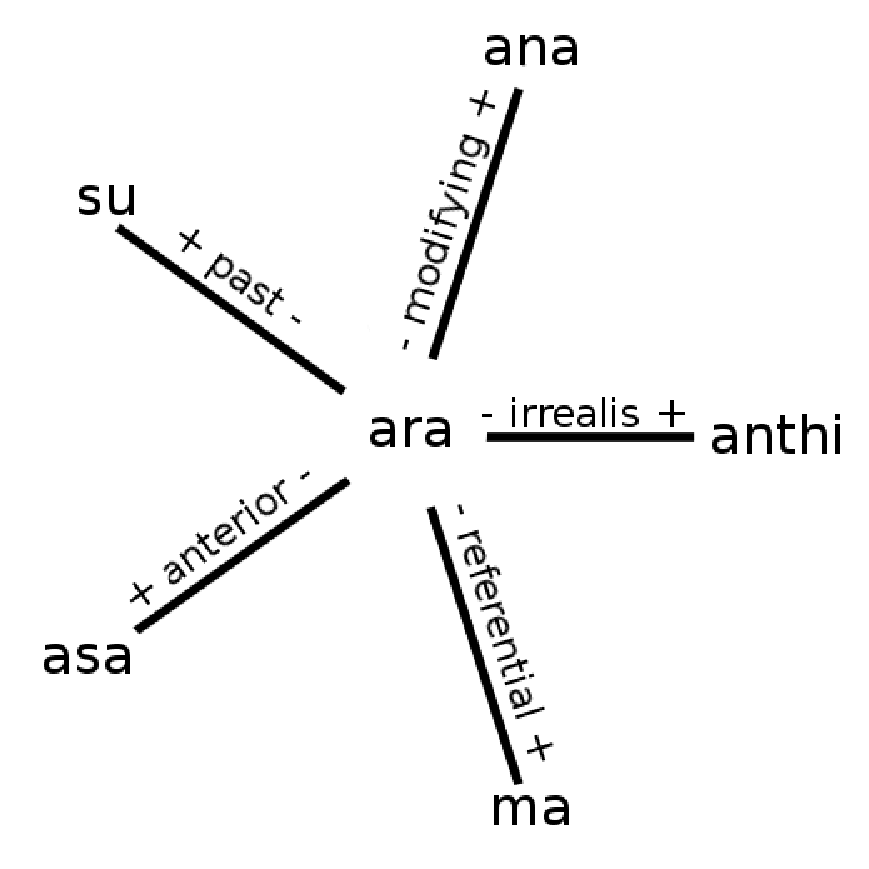
\includegraphics[width=.5\textwidth]{pics/Pentagram-ara.eps}
% 	\caption{$ arà\div$ as the unmarked choice in the semantic space of tense and modality}
% 	\label{fig:Pentagram-ara}
% \end{figure}

\subsection{Inflectional suffixes}\label{sec:morph:Inflectionalsuffixes}
Both inflectional suffixes in SLM are imperative markers. \em -la \em is a polite imperative, while \em -de \em is an impolite imperative.

\subsubsection{imperative \em-la\em}\label{sec:morph:-la}
This suffix is an imperative marker which attaches to a verbal host. It is used for command clauses \funcref{sec:pragm:Requestingaction}. It has no influence on vowel lengthening processes. This morpheme can be used on its own on a verb \xref{ex:form:affix:la:solo}, or be combined with the imperative particle \em mari\em, which reinforces its meaning \xref{ex:form:affix:la:double}.



% \xbox{16}{
% \ea\label{ex:form:unreferenced}
% \gll \textbf{Diya-la} {\em uncle}, se=ppe SSC {\em exam} mà-ambel=nang duva-pul aari su-aada. \\
%      see-\textsc{imp} uncle \textsc{1s}=\textsc{poss} SSC exam \textsc{inf}-take=\textsc{dat} two-ty day \textsc{past}-exist  \\
%     `See, uncle, there are (only) twenty days left until I will have take the SSC exam.'  (K051220nar01)
% \z      
% }\\ 



\xbox{16}{
\ea\label{ex:form:affix:la:solo}
\gll Allah \textbf{diyath-la} inni pompang pada dhaathang aada. \\
      Allah watch-\textsc{imp} \textsc{prox} female \textsc{pl} come exist \\
    `Almighty, see, that woman has come!' (K061019nar02)
\z
}


\xbox{16}{
\ea \label{ex:form:affix:la:double}
\ea
\gll Saayang se=ppe thuan \textbf{mari} laari-\textbf{la}. \\
      love \textsc{1s}=\textsc{poss} sir come.\textsc{imp} run-\textsc{imp} \\
    `Come my beloved gentleman, come here.'
\ex
\gll See=samma kumpul \textbf{mari} thaa\u ndak-\textbf{la}. \\
     \textsc{1s}=\textsc{comit} gather come.\textsc{imp} dance-\textsc{imp}  \\
    `Come and dance with me.' (N061124sng01)
\z
\z
}



This morpheme is reasonably frequent. It is cognate with  Std. Malay  \em lah, \em used for imperatives and emphasis.


\subsubsection{impolite imperative \em -de\em}\label{sec:morph:-de}
This morpheme is an impolite imperative suffix. This morpheme was only discovered at the evening of the very last day of elicitation in an informal setting without recording device. It is not found  in the corpus, which might be due to its very impolite connotations. The following example is the one which was given to illustrate its use.


\xbox{16}{
\ea
\gll Pii! ... pii!! ... pii-de!!! \\
     go ... go ... go-\textsc{imp.impolite}  \\
    `Go! Go now! Bugger off!!!' (not on recordings)
\z
}



\subsection{Derivational affixes}\label{sec:morph:Derivationalaffixes}
Sri Lanka Malay has two category-changing affixes: a nominalizer \em -an \em and a causativizer \em -king\em. In the verbal domain, there is a further involitive prefix \em kànà-\em,\footnote{There is a possibility of the existence of a prefix
	used to derive accidental verbs, \em tha-\em. This was overheard several times in the string \em as-tha \em, but at first misinterpreted as an allomorph of the conjunctive participle \em asà-\em, instead of the probably correct parsing \em asà+tha\em. This prefix has been found with the verb \trs{bunthur}{knock} and other highly transitive verbs. The morpheme might be related to the Standard Malay prefix \em ter- \em used to derive ``stative, accidental or habilitative verbs in [Standard Malay]'' (\citet{Paauw2004}, also see \citet{Adelaar2005struct}, and \citet[181]{Adelaar1985} on Jakartanese \em t\E-\em). As far as I can remember, in all the contexts where \em astha- \em occurred, a reading as `accidental' would have been semantically plausible. From the above description it should be clear that this morpheme, and its relations to \em kìnna \em \formref{sec:wc:vv:kinna} and \em kànà-, \em \formref{sec:morph:kana-} need further research.}
while in the nominal domain, we find a special suffix for kin of third person.
There is notably no affix deriving adjectives, but the clitic \em =ke \em \formref{sec:morph:=ke} could be used for this function.

\subsubsection{nominalizer \em -an\em}\label{sec:morph:-an}
This suffix can be used to derive nouns from verbs like \trs{maakang}{eat} (\trs{makanan}{food}) or adjectives like \trs{maanis}{sweet} (\trs{manisan}{sweets}) \citep[cf.][28]{Adelaar1991} \formref{sec:wofo:Nominalization}. The semantic result is not predictable. It can be an item (\em manisan, makanan\em) or an action like \trs{banthuan}{help}. When attached to a stem ending in front  vowel, \em y \em may be inserted (\trs{pake-y-an}{dress}). After a stem ending in \em a\em, \em h \em must be inserted (\trs{suka-h-an}{liking}). The result of the derivation is necessarily trisyllabic because all verbs are at least disyllabic.\footnote{With the exception of \trs{pii}{go}, but this verb cannot combine with \em -an\em.}
 
Words derived with \em -an \em never lengthen the penultimate vowel. This is not surprising, since there is normally enough material in the three syllables to construct a bimoraic foot even under extrametricality of the final syllable (ma$_{\mu}$.ka$_{\mu}.<$nan$>$) (see Section \ref{sec:phon:analysis:Stems}, p. \pageref{sec:phon:analysis:Stems}). A special case are the stems with a schwa in the initial syllables like \phonem{s@gar}[\textipa{sI$_{\mu}$g$_{\mu}$.$<$gar$>$}]`healthy'. These normally raise the schwa to generate one mora, and geminate the consonant, to generate another one. When derived with \em -an\em, the gemination tends to go away, while the schwa remains raised, thus \phonet{sI$_{\mu}$.ga$_{\mu}$.$<$ran$>$}`health'. Note that the /g/ is resyllabified in the derived word.
% 
% It is important to distinguish the derivational suffix \em -an \em from then dative enclitic \em =nang\em. This is sometimes difficult because the final nasals tend to velarize, so that \em -ang \em can be an allophone of \em -an\em. When an alveolar nasal is found, this is a clear sign for the
% 
% 
% So, the velar nasal is never distinctive, but a final alveolar nasal is a sure sign that the morpheme at hand is not \em =nang\em. Furthermore, vowel lengthening is canceled in \em-an\em-derivation, but remains with \em =nang\em. Finally, there is a geminate nasal when \em =nang \em is added to a stem ending in \em n. \em When \em -an \em is suffixed on such a suffix, the nasal remains simple and is resyllabified, so \em maa.kang.nang \em but \em ma.ka.nan(g)\em. The following example shows both the clitic and the nominalizer in one sentence, where we can see the different phonological effects
% 
% \xbox{16}{
% \ea\label{ex:form:an:annang}
% \gll Manis-\textbf{ang} maakang=\textbf{nang} go suuka bannyak. \\
%  sweet-\textsc{nmlzr} eat=\sc{dat} \textsc{1s.familiar} like much\\
% `I like very much to eat sweets.' (B060115prs20)
% \z	
% }
% 
% In the above example, \em manisan \em does not have a long vowel (compare \trs{maanis}{sweet}). It is syllabified $(ma_{\mu}.ni_{\mu}.<san>)_{\omega}$. \em maakangnang \em on the other hand does have that long vowel because it is syllabified as $(ma_{\mu}a_{\mu}.<kang>)_{\omega}(nang)_{\omega}$. Finally, there is only one consonant between the last two syllables in \em mani\textbf{s}an\em, but there are two of them in \em maaka\textbf{\ng n}ang\em.

This affix is directly inherited from the historical affix with the same form and function. There are also the related circumfixes \em pàr-...-an \em and \em ka-...-an\em, which are also nominalizers. These are no longer productive in Sri Lanka Malay and are treated as allomorphs of \em -an \em here.



% \xbox{16}{
% \ea\label{ex:form:unreferenced}
% \gll Tsunaami anà-jaadi     cupathan=nang kithang=nang   thàràthaau. \\
%       tsunami \textsc{past}-become quick-\textsc{nmlzr} \textsc{1s}=\textsc{dat} neg.know \\
%     `We did not know about the speed with which the tsunami came.' (B060115nar02)(test)
% \z
% } \\ \

The use of \em -an \em can be seen in several instances in \xref{ex:form:-an:triple} where the verbs \trs{aajar}{teach} and \trs{thaksir}{think} are derived by this suffix. The last form, \trs{plajaran}{lesson}, bears resemblance to the expected form \em *blajaran\em, derived from \trs{blaajar}{learn}, but the initial consonant is voiceless. This is thus an irregular nominalization. The reason for this irregularity is the historic derivation \em pe-...-an\em, which has reflexes in Modern Indonesian \em pelajaran\em. This derivation by \em pe-...-an \em also has  different semantics, since we are not dealing with acquiring knowledge, but with imparting knowledge.


\xbox{16}{
\ea\label{ex:form:-an:triple}
\ea 
\gll Derang=pe \textbf{ajar-an} bannyak baaye. \\
     \textsc{3pl}=\textsc{poss} teach-\textsc{nmlzr} much  good  \\
    `Their teaching was very good.'  
\ex
\gll Derang=pe \textbf{thaksir-an}=le bannyak baaye. \\
     \textsc{3pl}=\textsc{poss} think-\textsc{nmlzr} much good   \\
    `Their thoughts were very good.' 
\ex
\gll Derang=pe \textbf{plajaran}  bannyak baaye. \\
     \textsc{3pl}=\textsc{poss} lesson much good   \\
    `Their lessons were very good.' (K051213nar03)
\z
\z
}


Nominalized verbs may continue to govern arguments, as example \xref{ex:form:-an:arguments} shows.

\xbox{16}{
\ea\label{ex:form:-an:arguments}
\gll Lorang=nang \textbf{see=yang} ingath\textbf{-an}=si. \\
     \textsc{2pl}=\textsc{dat} \textsc{1s}=\textsc{acc} remember-\textsc{nmlzr}=\textsc{interr} \\
    `Do you remember me?'  (K070000wrt04)
\z      
}

In this example, the verb \trs{iingath}{think} governs the accusative, and this remains even after nominalization. This contrasts with English, where arguments of nominalized verbs obligatorily take the genitive  (\em Do you have remembrance/memories \textbf{of} me\em).

An interesting case of the interplay of word classes and the nominalizer is the word \em jaalang\em. \em Jaalang \em can either be used as a verb with the meaning `to walk', as in \xref{ex:form:jaalang:walk}. It can also be used as a noun with the meaning `street', which is obviously related semantically, but not enough to warrant an analysis as conversion because the meaning of `street' is much more restricted than the meaning of `walk'. Finally, the verb \trs{jaalang}{walk} can be derived by \em -an \em to yield the word \trs{jalangan}{trip} \xref{ex:form:jalang:jalangan}.


\xbox{16}{
\ea\label{ex:form:jaalang:walk}
\ea
\gll Katugastota=nang   {\em train}=ka asà-dhaathang. \\ % bf
     Katugastota=\textsc{dat} train=\textsc{loc} \textsc{cp}-come  \\
    `I arrived in Katugastota by train.' 
\ex
\gll Katugastota asàduuduk {\em St.Anthony's}=nang     \textbf{arà-jaalang} \\
     Katugastota from St.Anthony's=\textsc{dat} \textsc{non.past}-walk  \\
    `(Then) I used to walked from Katugastota (train station) to St. Anthony's (school).' (K051201nar02)
\z
\z
}

\xbox{16}{
\ea\label{ex:form:jalang:street}
\gll kàthaama kithang kiccil muusing=ka, inni     \textbf{Peeradheniya} \textbf{Jaalang}=ka  samma an-aada      mlaayu. \\
     before \textsc{1pl} small time=\textsc{loc} \textsc{prox} Peradeniya street=\textsc{loc} all \textsc{past}-exist Malay  \\
    `Before, when we were children, it was all Malays here on Peradeniya Rd.' (K051222nar04)
\z
}

\xbox{16}{
\ea\label{ex:form:jalang:jalangan}
\gll \textbf{jalang-an} hatthu arà-pii vakthu \\
    walk-\textsc{nmlzr} \textsc{indef} \textsc{non.past}-go time    \\
    `when we go on a trip' (K051213nar06)
\z
}



% \xbox{16}{
% \ea\label{ex:form:unreferenced}
% \gll Luu asà-bìssar apa lu=ppe umma-baapa=nang kaasi \textbf{sayang-an}. \\
%       \textsc{2s.familiar} \textsc{cp}-big after \textsc{2s}=\textsc{poss} mother-father=\textsc{dat} give love-\textsc{nmlzr} \\
%     `When you will have grown up, give love to your parents.' (K060116sng01)%doubt
% \z
% } \\

In rare cases can \em -an \em be found on nouns, like \trs{raja-han}{king'+`\textsc{nmlzr}'=`government}. This is another use of \em -an\em, also found in Standard Malay, and indicates `collectivity' or `similarity'  when attached to nouns, according to \citet[193]{Adelaar1985}. This meaning seems to be at hand here as well, where a government can be seen as a collection of kings, or similar to a king.

There is one instance of a nominalization after inflection, namely \trs{thradahan}{deprivation}, which is composed of the negative quasi-prefix \em thàrà$\div$\em, the existential \em aada, \em and the nominalizer. The non-negated form \trs{adahan}{possession} also exists. One could argue that the negation takes place after derivation, however, \em th(à)rà- \em is not a morpheme which can attach to nouns, so that  \em th(à)rà- \em must have been joined with \em a(a)da \em before the derivation.

%  se=ppe thradahaan subbath bannyak mlaarath
% 
% inciyangpe thradahaan duvithka bukang, thumpath.
% 
% inciyangpe adahan kubbong. 3.08
% 
% 

\subsubsection{causativizer \em -king\em}\label{sec:morph:-king}
This causative morpheme  can derive verbs from  adjectives and verbs \formref{sec:wofo:Causativization}. It has an alternative realization \em -kang\em, which seems to depend on phonological environment, but also on speakers.
\citet[29]{Adelaar1991} proposes that this morpheme might either be a reflex of the transitivizing suffix \em -k\E n \em found in non-standard forms of Malay and Javanese, or derived from \trs{biki\ng}{to do, make}. It might also be the case that \em -kang \em is related to \em -k\E n \em and \em -king, \em to \em biking\em.

In most cases, both \em -king \em and \em -kang \em are possible in SLM \citep[cf.][60]{Saldin2001}. 
The cases where some speakers feel only one is possible are highly unsystematic and do not lend themselves to an easy categorization.

One and the same speaker can use then one allomorph, then the other with the same base in comparable contexts. The same writer uses \trs{encoking}{fool(V)} consistently in one text (K070000wrt02) and \trs{encokang}{fool(V)} in another one (K070000wrt05).


\xbox{16}{
\ea
\gll [Andare=yang   mà-\textbf{enco-king}=nang]        raaja su-biilang     [itthu    paasir katha]. \\
      Andare=\textsc{acc} \textsc{inf}-fool-\textsc{caus}=\textsc{dat} king \textsc{past}-say \textsc{dist} sand \textsc{quot} \\
    `To fool Andare, the king said that this was sand.' (K070000wrt02)
\z
}

\xbox{16}{
\ea \label{ex:form:king:encokang}
\gll Kanabisan=ka=jo duva oorang=le anà-thaau ambel [Andare duva oorang=yang=le asà-\textbf{enco-kang} aada] katha. \\
      last=\textsc{loc}=\textsc{emph} two man=\textsc{addit} \textsc{past}-know take Andare two man=\textsc{acc}=\textsc{addit} \textsc{cp}-fool-\textsc{caus} exist \textsc{emph} \\
    `At the very end, both women understood that Andare had fooled both of them.' (K070000wrt05)
\z
}


% \xbox{16}{
% \ea\label{ex:form:unreferenced}
% \gll Dee su-baavung-\textbf{kang}       baapa-yang. \\
%       \sc{3s} \sc{past}-rise-\sc{caus} father-\sc{hypoc} \\
%     `He lifted daddy.' (K051205nar05)
% \z
% } \\





Table \ref{tab:form:kingkang} gives the instances of verbs derived by \em -king \em and \em -kang \em in the corpus, excluding loanwords.

\begin{table}
\begin{center}
% use packages: array
\begin{tabular}{ll}
 -king  &   -kang \\
\hline
\trs{abbis-king}{finish+\textsc{caus}=fulfill (a wish)} 		& \trs{bava-kang}{bring+\textsc{caus}=have s.o. bring}  \\
\trs{bale(k)-king}{turn (intr)+\textsc{caus}=(re)turn (tr)} 	& \trs{bavung-kang}{rise+\textsc{caus}=lift} \\
\trs{biilang-king}{say+\textsc{caus}=make say} 				& \trs{binthi-kang}{stop (intr)+\textsc{caus}=stop (tr)} \\
\trs{blajar-king}{learn+\textsc{caus}=teach} 			& \trs{buunan-kang}{kill+\textsc{caus}=have killed} \\
\trs{buunung-king}{kill+\textsc{caus}=have s.o. killed} 			& \trs{dudu-kang}{sit+\textsc{caus}=put down} \\
\trs{enco-king}{fooled+\textsc{caus}=fool (V)} 			& \trs{enco-kang}{fooled+\textsc{caus}=fool(tr)} \\
\trs{jadi-king}{become+\textsc{caus}=grow, run (a business)} 	& \trs{gaa\u ndas-kang}{connected+\textsc{caus}=connect} \\
\trs{kasi-king}{give+\textsc{caus}=make give} 			& \trs{gijja-kang}{make+\textsc{caus}=have s.o. make} \\
\trs{kaving-king}{marry+\textsc{caus}=marry off} 		& \trs{hina-kang}{embarrassed+\textsc{caus}=embarrass} \\
\trs{kubuur-king}{buried+\textsc{caus}=bury} 			& \trs{iingath-kang}{think+\textsc{caus}=recall} \\
\trs{mandi-king}{bathe+\textsc{caus}=wash} 			& \trs{livath-kang}{exceed+\textsc{caus}=increase} \\
\trs{mathi-king}{dead+\textsc{caus}=kill} 			& \trs{jalang-kang}{walk+run=run (a business, country)} \\
\trs{salba-king}{escape+\textsc{caus}=liberate} 			& \trs{mathi-kang}{dead+\textsc{caus}=kill} \\
\trs{thau-king}{know+\textsc{caus}=inform}			& \trs{korban-kang}{sacrifice(n)+\textsc{caus}=sacrifice} \\
\trs{thumpa-king}{spill (intr)+\textsc{caus}=spill (tr)} 		& \trs{kubuur-kang}{buried+\textsc{caus}=bury} \\
 \trs{mlidi-king}{boil (intr)+\textsc{caus}=boil (tr)} 	 & \trs{luppas-kang}{leave+\textsc{caus}=leave sth. behind}  \\
 \trs{panas-king}{hot+\textsc{caus}=heat} 	 & \trs{picca-kang}{broken+\textsc{caus}=break} \\
 \trs{thurung-king}{descend+\textsc{caus}=lower} 	 & \trs{punnu-kang}{full+\textsc{caus}=fill} \\
 							& \trs{rubbus-kang}{boil (intr)+\textsc{caus}=boil (tr)} \\
 							& \trs{salba-kang}{escape+\textsc{caus}=liberate} \\
 							& \trs{sakith-kang}{sick+\textsc{caus}=hurt (tr)} \\
 							& \trs{vaasil-kang}{blessed+\textsc{caus}=bless} \\
\end{tabular}
\end{center}
\caption{The use of \em -king \em and \em -kang \em on different bases in the corpus.}
\label{tab:form:kingkang}
\end{table}



A special case is the word for `to show' (\em cunjikang, thunjiking\em), which has a causative morpheme, but whose base is synchronically not transparent. It is not clear whether a swap of \em king \em for \em kang \em in this pair would be possible.

As for its phonological status, \label{page:morph:king} \em -king \em is in a middle position between an affix and a clitic. Just like affixes, it is selective with regard of its host and its position. \em -king \em cannot be preposed or otherwise moved around in the clause, it cannot occur on its own and it can only attach to adjectives and verbs. For some speakers, \em -king \em has the same metrical properties as \em -an\em, while for others \em -king \em is not parsed into the same phonological word as its stem, which has as a consequence that the penultimate syllable of the stem is lengthened. See \formref{sec:phon:Analysisofwordstructure} for a discussion. On a diachronic note, it appears that the original clitic status of \em -king \em is eroding and \em -king \em becomes grammaticalized as an affix.

The changing status of \em -king \em can also be retraced in the literature. My informants accept both short and long vowels, and produce both. On the other hand, Bichsel's informants  did not have \em -king \em within the word domain of the stem (i.e. they had vowel lengthening), while Tapovanaye's informants had \em -king \em within the word domain of the stem, preventing lengthening. This suggests that within the speaker population, there are people who assign one status to \em -king\em, another group assigns the other status, and a third one accepts and produces both.

As for its hosts, \em -king \em can be used on adjectives as in \xref{ex:king:adj1}\xref{ex:king:adj2}, with intransitive verbs as in \xref{ex:king:intrans1}\xref{ex:king:intrans2} and with transitive verbs as in \xref{ex:king:trans1}\xref{ex:king:trans2}.


\xbox{16}{
\ea \label{ex:king:adj1}
\gll Itthuka asà-thaaro, itthu=yang arà-\textbf{panas}$_{adj}$\textbf{-king}. \\
      \textsc{dist}=\textsc{loc} \textsc{cp}-put \textsc{dist}=\textsc{acc} \textsc{non.past}-hot-\textsc{caus} \\
    `Having put (it) there, you heat it.'  (B060115rcp02)
\z      
} 

\xbox{16}{
\ea \label{ex:king:adj2}
\gll Mà-mathi-king,  mà-\textbf{mathi}$_{adj}$\textbf{-king}=nang, siithu=jo anà-baapi. \\
      \textsc{inf}-dead-\textsc{caus} \textsc{inf}-dead-\textsc{caus}=\textsc{dat} there=\textsc{emph} \textsc{past}-bring \\
    `It was there that (they) brought (him) to make (him) dead.'  (K051206nar02)
\z      
} 

\xbox{16}{
\ea \label{ex:king:intrans1}
\gll Inni=ka inni daalang=ka kithang aayer masà-\textbf{mlidi}$_{intr}$\textbf{-king}. \\ % bf
  \textsc{prox}=\textsc{loc} \textsc{prox} inside=\textsc{loc} \textsc{1pl} water must=boil-\textsc{caus}     \\
    `On this, inside this, we must boil water/bring the water to a boil.'  (B060115rcp02)
\z      
} 

\xbox{16}{
\ea \label{ex:king:intrans2}
\gll Baaye meera caaya kapang-jaadi, \textbf{thurung}$_{intr}$\textbf{-king}. \\
     good red colour when-become, descend-\textsc{caus}  \\ % bf
    `When  [the food] has  turned to a nice rose colour, remove (it) [from the fire].'  (K060103rec02)
\z      
}
 
\xbox{16}{
\ea \label{ex:king:trans1}
\gll De laaye hathu nigiri=nang anà-baapi, \textbf{buunung}$_{tr}$\textbf{-king}=nang. \\ % bf
      3\textsc{s.impolite} other \textsc{indef} country=\textsc{dat} \textsc{past}-bring kill-\textsc{caus}=\textsc{dat}\\
    `They brought him to another country to have him executed.'  (K051206nar02)
\z      
} 

\xbox{16}{
\ea \label{ex:king:trans2}
\ea 
\gll Suda maven=subbath see anà-{\em resign}. \\ % bf
     so son=because \textsc{1s} \textsc{past}-resign  \\
    `So I quit because of my son.'   
\ex
\gll Maven masà-\textbf{blajar}$_{tr}$\textbf{-king}=jona. \\ % bf
     son must-learn-\textsc{caus}=\textsc{emph}=\textsc{phat}  \\
    `Well, somebody has to teach him, isn't it.'  (B060115prs21,K081105eli02)
\z 
\z     
}


Besides the normal use of \em -king \em on verbs or adjectives, there are two less common bases in the corpus, a noun \xref{ex:form:king:kafan} and a particle \xref{ex:form:king:thraa}. In \xref{ex:form:king:kafan}, the noun \trs{kafan}{shroud} is derived with \em -king \em to yield \trs{kafan-king}{enshroud}.



\xbox{16}{
\ea\label{ex:form:king:kafan}
\gll Spaaman=yang   asà-\textbf{kafan}-\textbf{king} spaaman=yang   sithu=ka nya-kubuur-king. \\
     \textsc{3s.polite}=\textsc{acc} \textsc{cp}-shroud-\textsc{caus} \textsc{3s.polite}=\textsc{acc} there=\textsc{loc} \textsc{past}-buried-\textsc{caus}  \\
    `The body was wrapped in cloth and then the body was finally buried.' (B060115nar05)
\z
}

% itthu    blaakang sithu=ka=jo
% spaaman suda aayer  samma asà-kumpul
% spaaman=yang   asà-mandi-king
% spaaman=yang   asà-kafan-king spaaman=yang   sithu=ka nya-kubuur-king
% `After that, right there, the water was collected and then the body was bathed and then the body was wrapped in cloth and then the body was finally buried.'

In \xref{ex:form:king:thraa}, the negative particle \em thraa \em is used as a base of \em -king \em to yield \trs{thraa-king}{get rid of}.

\xbox{16}{
\ea\label{ex:form:king:thraa}
\gll Itthu=nang, kithang arà-thraa-king, kithang=pe Seelon=pe mosthor=nang. \\
      \textsc{dist}=\textsc{dat} \textsc{1pl} \textsc{non.past}-\textsc{neg}-\textsc{caus} \textsc{1pl}=\textsc{poss} Ceylon=\textsc{poss} manner=\textsc{dat}  \\
    `Therefore, according to the Sri Lankan way, we are getting rid of that.' (B060115rcp01,K081103eli02)
\z
}
 
\em -king/-kang \em is also the standard way to integrate English loan verbs. Note that there is no causation involved, so \em serve-king \em means `to serve' and not `make serve'. The following example shows extensive use of this pattern in the explanation of the rules of sepaktakraw, which is a rather recent sport in Sri Lanka, and the terminology used (serve, break, set, smash) is borrowed from English volleyball terminology.


\xbox{16}{
\ea\label{ex:form:king:loan:triple}
\ea 
\gll Itthu=yang \textbf{{\em serve}-king}  atthyang subla=dering arà-\textbf{{\em break}-king}. \\
      \textsc{dist}=\textsc{acc} serve-\textsc{caus}  other side=\textsc{abl} \textsc{non.past}-break-\textsc{caus} \\
    `Serve the ball, on the other side they break the ball.'
\ex
\gll \textbf{{\em Break}-king}=apa, kithang arà-\textbf{{\em set}-king}. \\
      break-\textsc{caus}=after \textsc{1pl} \textsc{non.past}-set-\textsc{caus} \\
    `After breaking, we set the ball.' 
\ex
\gll \textbf{{\em Set}-king}=apa arà-\textbf{{\em smash}-king}. \\
     set-\textsc{caus}=after \textsc{non.past}-smash-\textsc{caus}  \\
    `After setting, we smash the ball.' (N060113nar05)
\z
\z
}

Table \ref{tab:form:kingkang:loan} shows the loan verbs found in the corpus which bear this morpheme.

\begin{table} 
\begin{center}
% use packages: array
\begin{tabular}{ll|ll}
\multicolumn{2}{c}{-king}&\multicolumn{2}{c}{-kang}\\
capture-king 	& serve-king   	& admit-kang 	& organize-kang \\
bomb-king 	& dub-king 	& attack-kang 	& mix-kang 	\\
conduct-king 	& smash-king 	& boil-kang 	& introduce-kang \\
perform-king 	& break-king 	& celebrate-kang & print-kang   \\
play-king 	& introduce-king & follow-kang 	& execute-kang \\
select-king 	& bat-king 	&  force-kang  	& represent-kang \\
thanks-king 	& bowl-king 	& sacrifice-kang & mix-kang 	\\
set-king 	& spend-king 	& wrap-kang 	& curse-kang 	\\
issue-king 	&    		&  	 	&  set-kang	\\
\end{tabular}
\end{center}
\caption{The use of \em -king \em and \em -kang \em on different loanwords in the corpus.}
\label{tab:form:kingkang:loan}
\end{table}


% K060116nar10
% Kluu\u mbu oorang pukijja  boolekang   gijja no ,meaning 5.11.08





% \xbox{16}{
% \ea
% \gll Kithang samma oorang mlaayu padanang   biilangkingapajo. \\
%        \\
%     `We have informed all the other Malays.' (nosource)B060115nar02.txt: better kasithaau
% \z
% } \\

% 
% 
% \xbox{16}{
% \ea\label{ex:form:unreferenced}
% \gll Incayang pe malacca {\em chief} {\em minister}'s {\em visit}=nang lunch hatthu=nang incayang 60,000 nya-blaanja-kang. \\
%       \textsc{3s.polite}=\textsc{poss} Malacca chief minister's visit=\textsc{dat} lunch \textsc{indef}=\textsc{dat} \textsc{3s.polite} 60,000 \textsc{past}-pay-\textsc{caus} \\
%     `.' (K060116nar07)
% \z
% } \\
%  





\subsubsection{involitive \em kànà-\em}\label{sec:morph:kana-}

\em Kànà- \em is a morpheme used to derive involitive verbs from volitive verbs \formref{sec:wofo:Involitivederivation}. The verbs thus derived govern the dative.  This morpheme is not very frequent, and it was difficult to get solid information about its use. The following two examples show the schematic use.


\xbox{16}{
\ea
\gll Se naasi arà-maakang. \\ %bf
     \textsc{1s} rice \textsc{non.past}-eat  \\
    `I eat rice.' (K081104eli03)
\z
} \\ 

\xbox{16}{
\ea
\gll Se=dang naasi arà-\textbf{kànà}-maakang. \\
     \textsc{1s=dat} rice \textsc{non.past}-\textsc{invol}-eat  \\
    `I eat rice without wanting it/I compulsively eat rice/I was forced to eat rice by something beyond my control.' (K081104eli03)
\z
}


Some semantically primary verbs, like \trs{bangkas}{sneeze} can also take \em kànà-\em. In this example, the verb does not seem to be derived from a volitive verb.

% sneeze % 04110103
\xbox{14}{
\ea
\gll Sedang arà-\textbf{kànà}-bangkas  \\
     \textsc{1s.dat} \textsc{non.past}-\textsc{invol}-sneeze  \\
    `I sneeze.' (K081104eli03)
\z
}


It appears that \em kànà- \em is used to emulate the Sinhala involitive conjugation class in \em -enavaa\em, which also governs the dative \citep{Gair1971actioninvolvement}. The semantics of the verbs of this class in Sinhala are treated in detail in \citet{Gair1971actioninvolvement} as well, which might be an interesting point of departure for the semantic analysis of \em kànà-\em.

\em Kànà- \em can also be used with intransitive verbs \xref{ex:form:kana:pii}. In this case, the dative marking can be left out.

\xbox{16}{
\ea\label{ex:form:kana:pii}
\gll Incayang su-kànà-pii. \\
     \textsc{3s.polite} \textsc{past}-\textsc{invol}-go  \\
    `He left inadvertently/He left without wanting it/He left because of something beyond his control.' (K081104eli03)
\z
}

It is possible that this prefix is related to the vector verb \em kìnna\em, which has very similar semantics. The difference is that \em kànà- \em changes the argument structure of the verb, which governs the dative after derivation with \em kànà-\em. \em Kìnna \em on the other hand, leaves the argument structure of the verb unaffected \formref{sec:wc:vv:kinna}. This suggests that these two morphemes are not allomorphs. \em kànà- \em changes the morphosyntactic properties of a verb, while \em kìnna \em only emphasizes a certain semantic aspect. The fact that these two morphemes are not allomorphs can also be seen by their possibility to co-occur, as in \xref{ex:form:kana:kinna}.

  
\xbox{14}{
\ea\label{ex:form:kana:kinna}
\gll Itthu haari=ka=jo aanak pompang duuva=nang hathu duuri pohong=nang   jee\u n\u ggoth=yang anà-\textbf{kànà}-daapath \textbf{kìnna} hathu  Aajuth hatthu=yang su-kuthumung.   \\
     \textsc{dist} day=\textsc{loc}=\textsc{emph} child female two=\textsc{dat} \textsc{indef} thorn tree=\textsc{dat}   beard=\textsc{acc} \textsc{past}-\textsc{invol}-get strike \textsc{indef}   dwarf \textsc{indef}=\textsc{acc} \textsc{past}-see  \\
    `On the same day, the two girls  saw a   dwarf whose   beard had got stuck  in a thorn tree.' (K070000wrt04)
\z
}

In \xref{ex:form:kana:kinna}, \em kànà- \em marks the involitive nature of getting stuck, while \em kìnna \em adds a shade of adversative surprise. It is nevertheless likely that both these morphemes are cognate to the Std. Malay \em k\E na, \em which can be used for adversative passives \citep{Chung2005kena}.




% \xbox{16}{
% \ea
% \gll Seeyang iblisnang su kànà daapath. \\
%        \\
%     `.' (nosource)19.11.2008
% \z
% } \\

% 
% \xbox{16}{
% \ea
% \gll Maldives ka baaru hatthu {\em president} asà kànà thiiri aada. \\
%        \\
%     `The new president of the Maldives has been elected.' (K08114eli01)
% \z
% } \\
% 
% 
% 
% \xbox{16}{
% \ea
% \gll Maldives ka baaru hatthu {\em president} asà kànà thiiri kìnna aada. \\
%        \\
%     `Surprisingly, the president was elected but did not know about it.' (K08114eli01)
% \z
% } \\



\subsubsection{kin term \em -yang\em}\label{sec:morph:-yang}
This is a derivational affix which can only attach to kin terms. The kin relation may not involve the speaker or the addressee. It must not be confounded with the homophonous direct object marker, the cliticized postposition \em =yang \em \formref{sec:morph:=yang}. The former is a derivational affix which indicates the kin relation, while the latter is an enclitic postposition indicating the semantic role of patient. The affix can occur in places where the postposition could not occur, e.g. with intransitives \xref{ex:form:affix:-yang:subject}. Furthermore, the suffix can be used on referents marked for other semantic roles, like in  example \xref{ex:form:affix:-yang:nang}, where the father is marked for dative with the postposition \em =nang\em. It would not be possible to stack the postposition \em =yang \em and the postposition \em =nang\em. Finally, the affix \em -yang \em and the postposition \em =yang \em can stack, which clearly shows that they are different morphemes \xref{ex:form:affix:-yang:yang}.

\xbox{16}{
\ea \label{ex:form:affix:-yang:subject}
\gll [Bapa-yang]$_{ag}$ arà-dhaathang. \\
     father-\textsc{kin.3} \textsc{non.past}-come  \\
    `His/her father is coming.'  (K081103eli04)
\z      
} 

\xbox{16}{
\ea\label{ex:form:affix:-yang:nang}
\gll Kake-yang bapa-\textbf{yang=nang} su-maaki. \\
      grandad-\textsc{kin.3} father-\textsc{kin.3}=\textsc{dat} \textsc{past}-scold \\
    `His grandad  scolded his father.'   (K081103eli04)
\z      
}

\xbox{16}{
\ea\label{ex:form:affix:-yang:yang}
\gll Kake-yang bapa-\textbf{yang=yang} su-buunung. \\
      grandad father-\textsc{kin.3}=\textsc{dat} \textsc{past}-kill \\
    `His grandad  killed his father.'   (K081103eli04)
\z      
}


Naturalistic examples of \em -yang \em being combined with a postposition are \xref{ex:form:affix:-yang:stack1} and  \xref{ex:form:affix:-yang:stack2}, where the genitive \em =pe \em follows the string \em yang\em, thereby excluding the possibility to analyze it as a postposition indicating patient.


\xbox{16}{
\ea\label{ex:form:affix:-yang:stack1}
\gll inni     umma-\textbf{yang=pe}            dhaatha \\
      \textsc{prox} mother-\textsc{kin.3}=\textsc{poss} elder.sister \\
    `this mom's elder sister' (K051220nar01)
\z
}
 
\xbox{16}{
\ea\label{ex:form:affix:-yang:stack2}
\gll derang=pe mama-\textbf{yang=pe} ruuma \\
      \textsc{3pl}=\textsc{poss} uncle-\textsc{kin.3}=\textsc{poss} house \\
    `their uncle's house' (B060115nar05)
\z
}

The use of \em -yang \em with intransitives in naturalistic speech is given in \xref{ex:form:-yang:intr}, where the only arguments of the two occurrences of \trs{nii\u n\u ggal}{die} carry the string \em yang\em, and both are terms of kin (\trs{biini}{wife} and \trs{umma}{mother}). The verb \trs{nii\u n\u ggal}{die} never assigns accusative case to its argument, so that the instance of \em yang \em we are dealing with here must be the affix \em -yang \em and not the postposition \em =yang\em. A further indication of this is the short vowel in \em bini\em, which can sometimes occur with affixes, but not with postpositions. For this see the analogous discussion of vowel length with \em -king \em above (p. \pageref{page:morph:king}.)
 
\xbox{16}{
 \ea\label{ex:form:-yang:intr}
   \gll Ithukang       bini-\textbf{yang}       nii\u n\u ggal=le       umma-\textbf{yang}        nii\u n\u ggal=le  aanak pada    caari  dhaathang. \\
    Then wife-\textsc{kin.3} die=\textsc{addit} mother-\textsc{kin.3} die=\textsc{addit} child \textsc{pl} search come \\
`So then the wife died and the mother died, still the children will come in search.' (K051220nar01,K081105eli02)
\z
} 

% 
% 
% \xbox{16}{
% \ea\label{ex:form:unreferenced}
% \gll Laaki=yan iidop  pada=nang asà-pii caari ruuma=nang asà-baa  masà-thaaro  baaram umma masà-baa thaaro. \\
%       husband-hypoc living \textsc{pl}=\textsc{dat} \textsc{cp}-go find house=\textsc{dat} \textsc{cp}-bring must-put goods mother must-bring put\\
%     `The husband goes to earn a living and brings it home and has to give it to the mother.' (K061122nar01)
% \z
% } \\
% 


Sometimes, it is difficult to decide whether a given instance of \em yang \em is the kin affix or the accusative postposition.  The reason for this is that both markers are optional. When a kin term is used as a patient, we cannot know whether the string \em yang \em indicates the kin relation of the person or its status as an undergoer without more context. An example of that is \xref{ex:form:affix-yang:ambig} where the father is introduced. Introduction is not a violent activity, making the use of the accusative marker unlikely, but still possible \funcref{sec:func:Patient}. On the other hand, the speaker does refer to the father of a third person, so that the kin affix would be a possibility. Given the long vowel in \em baapa\em, the accusative reading is more likely, though.

\xbox{18}{
\ea\label{ex:form:affix-yang:ambig}
\gll Blaakang see Zeenath=pe baapa\textbf{-yang/=yang} nya-introduce-kang Sebastian=nang. \\
      After \textsc{1s} Zeenath=\textsc{poss} father-kin/=\textsc{acc} \textsc{past}-introduce-\textsc{caus} Sebastian=\textsc{dat}\\
    `After that I introduced Zeenath's daddy to Sebastian.' (B060115cvs01)
\z
}

%  Table \ref{fig:yanghypoc} gives a list of all the lexemes with which this affix has been found to combine.
% \begin{figure}
% 	\begin{tabular}{lll}
% 	SLM 	& English & Source\\
% 	\hline
% 		baapa		&	father		&	\\
% 		umma		&	mother		&	\\
% 		laaki		&	husband		&	\\
% 		planthen	&	bridegroom	&	\\
% 		maama		&			&	\\
% 	\end{tabular}
% 	\caption{Lexemes that can take the hypocoristic \em -yang \em}
%   	\label{fig:yanghypoc}
% \end{figure}

\subsection{Numeral affixes}\label{sec:morph:Numeralaffixes}
In the numeral domain finally, there are three affixes, for `-ty', `-teen' and `-th'.

\subsubsection{\trs{-blas}{-teen}}\label{sec:morph:-blas}
This suffix is used to derive the numbers between 11 and 19. It is parsed within the same phonological word as the stem, so that no vowel lengthening takes place in \em dhla(*a)pan \em and \em li(*i)ma \em in the following two examples.


\xbox{16}{
\ea\label{ex:form:blas:18}
\gll Suda se=ppe thuuva anak klaaki asàdhaathang \textbf{dhlapan-blas} thaaun. \\
       so \textsc{1s}=\textsc{poss} old child boy \textsc{copula} eight-teen year\\
    `So, my eldest son is eighteen.'  (K060108nar02)
\z      
} 
 
\xbox{16}{
\ea\label{ex:form:blas:15}
\gll Hathu \textbf{lima-blas} thaaun=nang duppang. \\
     \textsc{indef} five-teen year=\textsc{dat} before \\
    `About fifteen years before.'  (K061026prs01)
\z      
} 


\subsubsection{\trs{-pulu}{-ty}}\label{sec:morph:-pulu}
This suffix is used to derive the multiples of ten between 20 and 90. It is also parsed in the same phonological word domain as the stem, so that no lengthening takes place. Note the two occurrences of \em du(u)va \em in the following example, where one occurs with \em -pulu \em  and is not lengthhened, while the other one occurs on its own and is lengthened. Also note the short \em i \em in \em limapulu\em.


\xbox{16}{
\ea\label{ex:form:pulu:26452}
\gll \textbf{Duva-pulu} ìnnam riibu umpath raathus lima-pulu \textbf{duuva} {\em votes} incayang=nang anà-daapath. \\
     two-ty six thousand four hundred five-ty two votes \textsc{3s.polite}=\textsc{dat} \textsc{past}-get \\
    `He got 26,452 votes.'  (N061124sng01)
\z      
} 

% A partial phonological parsing of this sequence would be \xref{ex:form:26452:parsing}.
% 
% \xbox{16}{
% \ea\label{ex:form:26452:parsing}
% (du$_{??}$wa$_{\mu}$pu$_{\mu}$ $<$lu$>$)$_{\omega}$\\
% \parbox{0.2cm}{~}(\textipa{I}$_{\mu}$n$_{\mu}$ $<$nam$>$ )$_{\omega}$\\
% \parbox{0.4cm}{~}(ri$_{\mu}$i$_{\mu}$ $<$ bu $>$ )$_{\omega}$\\
% \parbox{0.6cm}{~}(\textipa{I}$_{\mu}$m$_{\mu}$ $<$path$>$ )$_{\omega}$\\
% \parbox{0.8cm}{~}(ra$_{\mu}$a$_{\mu}$ $<$ thus $>$ )$_{\omega}$\\
% \parbox{1.0cm}{~}(li$_{??}$ma$_{\mu}$pu$_{\mu}$ $<$lu$>$ )$_{\omega}$\\
% \parbox{1.2cm}{~}(du$_{\mu}$u$_{\mu}$ $<$wa$>$ )$_{\omega}$
% \z    
% }\\ 


\subsubsection{ordinalizer \em ka-\em}\label{sec:morph:ka-}
\em Ka- \em is  a prefix used to derive ordinals from cardinal numbers \citep[28]{Adelaar1991}. The vowel can be /a/ \xref{ex:form:ka-:ka} or schwa \xref{ex:form:ka-:ke}.

\xbox{16}{
\ea\label{ex:form:ka-:ka}
\gll Se   asdhaathangpa kitham=pe  femili=ka  \textbf{ka}-duuva aanak. \\
 \textsc{1s} \textsc{copula} \textsc{1pl}=\textsc{poss} family=\textsc{loc} \textsc{ord}-two child\\
`I am our family's second child.' (K060108nar01)
\z
}


\xbox{16}{
\ea\label{ex:form:ka-:ke}
\gll \textbf{Kà}-thiiga  {\em member} inni     kitham=pe      {\em legislative} {\em council}=ka. \\
      \textsc{ord}-three member \textsc{prox} \textsc{1pl}=\textsc{poss} legislative council=\textsc{loc} \\
    `He was the third member in this legislative council here.' (N061031nar01)
\z
}

\em Ka-\em, like all prefixes,  is ignored when calculating the moraic weight. This means that penultimate vowel lengthening takes place as normal. This is shown in \trs{(ka-)thuuju}{seven(-th)} in  \xref{ex:ka-:length}.



\xbox{16}{
\ea\label{ex:ka-:length}
\gll Se karang thuuju, ka-th\textbf{uu}ju thaaun=ka. \\
 \textsc{1s} now seven, \textsc{ord}-seven year=\textsc{loc} \\
`I am now in 7th grade.' (K060108nar01)
\z
}

The numerals \trs{ùmpath}{four}{} and \trs{ìnnam}{six} are realized by some speakers without the initial schwa, i.e. these numbers start with a syllabic nasal(\phonet{\s m.pa\dentt, \s n.nam}). This nasal  is \em not \em resyllabified when \em ka- \em is prefixed, so that the resulting word has three syllables (\phonet{ka.\s m.pa\dentt, ka.\s n.nam}).

\xbox{16}{
\ea\label{ex:form:ka-:umpath}
\gll Se Seelon dìkkath karang \textbf{ka-(ù)mpath} {\em generation}. \\
 \textsc{1s} Ceylon at now \textsc{ord}-four generation\\
`I am in Ceylon for the fourth generation.' (K060108nar02)
\z
}
 




\section{Simple clitics}\label{sec:morph:Simpleclitics}
Simple clitics are cliticized variants of words that can otherwise occur as a free form. In SLM, the cliticized forms of the modal particles, i.e. \em bolle=, bol=, bàr(à)= \em for \trs{boole}{can} and \em mau= \em for \em (ka)mau(van) \em fall under this category. Furthermore, the proclitic form \em kal= \em of the conditional particle \em kalu \em can also be analyzed as a simple clitic. Depending on the analysis of the quasi-prefixes, the number of simple clitics could increase. If the quasi-prefixes are regarded as free words because they can take the enclitic emphatic marker \em =jo\em, then  the reduced forms \em ar, at(t)hi, thi, mas(s)a, mas \em and \em thàr \em would also have to be analyzed as simple clitics.

\section{Bound words}\label{sec:morph:Boundwords}
SLM bound words are defined as words that cannot occur on their own, nor do they have a free form. They obligatorily need a host to which they can attach. What distinguishes them from affixes is that they are not selective with regard to their host. In SLM, all bound words attach to the right of the host, with the exception of the indefiniteness clitic \em (=)atthu(=) \em which can attach at both sides. No bound word interferes with the normal vowel lengthening pattern of the stem.

Bound words which attach to the NPs are
\begin{itemize}
 \item the indefiniteness clitic \formref{sec:morph:Indefinitenessclitic},
 \item the plural clitic \formref{sec:morph:Pluralclitic},
 \item   postpositions \formref{sec:morph:Postpositions}
 \item  prepositions \formref{sec:morph:Prepositions}.
\end{itemize}





Bound words which can attach to NPs, but also to predicates or clauses are
\begin{itemize}
 \item the Coordinating Clitics \formref{sec:morph:CoordinatingClitics},
 \item the informations structure clitics \formref{sec:morph:Focusclitics},
 \item and the evidential clitic \formref{sec:morph:kiyang}.
\end{itemize}


The last clitic, the quotative \em katha\em, attaches to the last word of an utterance \formref{sec:morph:katha}.

Bound words hail from a wide variety of semantic domains. Because of this, they do not compete for the same slots in the utterance and can be stacked quite well. The following example shows three clitics stacked on \em Malaysia\em.


\xbox{16}{
\ea\label{ex:form:boundwords:stack:natural}
\gll Seelon=pe=lle         mlaayu=nang {\em Malaysia}=\textbf{pe}=\textbf{lle}=\textbf{nang}   konnyon  {\em different}. \\
      Ceylon=\textsc{poss}=\textsc{addit} Malay=\textsc{dat} Malaysia=\textsc{poss}=\textsc{addit}=\textsc{dat} few different \\
    `Sri Lankan Malay and Malaysian Malay are a little bit different.' (B060115cvs09)
\z
}
 
The following constructed example shows the theoretical maximum of seven clitics. This is highly unnatural.


\xbox{16}{
\ea\label{ex:form:boundwords:stacking}
\glll ?[incayang  anà-pii  [aanak =pada =pe \zero{}(pàrhaal)  =subbath] =le    =jo  =kiyang  =katha] see su-biilang. \\
     \textsc{3s.polite} \textsc{past}-go child =\textsc{pl}   =\textsc{poss} {}       =because  =\textsc{addit} =\textsc{emph} =\textsc{evid}     =\textsc{quot} \textsc{1s} \textsc{past}-say  \\
     {}         {}     {}    deriv term {}       prop.cont infstr infstr interpersonal utterance {} {}			\\					
    `I said that it was reportedly also because of the children's [problems] that he left.'  (constructed) (K081103eli04)
\z      
} 


Note that the first three clitics (within the brackets) attach to  N(P) and carry propositional content The following two (\em =le \em and \em =jo\em), attach also to the NP, but indicate no propositional content but discourse function (additive focus and general focus). The next clitic \em =kiyang \em indicates evidential modality, a speaker attitude, and has thus bearing on the interpersonal leel, not indicating either propositional content or discourse function, but the speaker's relation to  the proposition he is using in his speech act. This can be seen from the fact that \trs{anàpii}{left} can be placed between \em =jo \em and \em =kiyang\em. Finally, \em katha \em is used to embed the whole reported utterance in a matrix sentence.
We can illustrate this as in \xref{ex:clitics:fgschema}, where we see at what levels the different clitics attach.

 
\ea \label{ex:clitics:fgschema}
% \begin{picture}(99,77)(0,0)
% \put(0,30){
$ 
\framebox{
	\framebox{
		\framebox{
			\framebox{
				\framebox{N (pl)}_{N}
			(poss)}_{NP}
		(postp)}_{PP}
	(coord)(focus)}_{msg} ...
(evid)}_{speech~act}
$
(quot)
% \end{picture}
\z

This schema should allow us to make neat predictions about the possible orders of clitics we can find. A clitic on an outer layer should never precede a clitic on an inner layer. This prediction is borne out. The only exception to this is the focus clitic \em =jo\em, which can also
be found attached to an utterance, i.e. at the rightmost position. An example is given in \xref{ex:form:boundwords:stacking:contra}. Note that there are two occurrences of \em =jo \em in this example, we are only interested in the last one.

\xbox{14}{
\ea\label{ex:form:boundwords:stacking:contra}
\gll [Dee=ka itthu=jo anà-aada \textbf{katha}]$_{ill}$=\textbf{jo}    arà-biilang \\
     3\textsc{s.impolite}=\textsc{loc} \textsc{dist}=\textsc{emph} \textsc{past}-exist \textsc{quot}=\textsc{emph} non.past-say  .\\
    `It is said that it was that what he had with him.' (K051206nar02)
\z
}

However, the utterance \trs{deeka    itthujo       anàaada}{it is that what he had with him} is embedded as an argument of \trs{biilang}{say} in the superordinate clause by \em katha\em, so that \em =jo \em in this case attaches to the argument as we would expect, and only indirectly to the utterance. This is shown in \xref{ex:clitics:fgschema:apply}.

\ea \label{ex:clitics:fgschema:apply}
$ 
\fbox{
\fbox{
\fbox{
\fbox{
\fbox{
\fbox{
 deeka    itthujo       anàaada    
}_{msg}
}_{speech~act}
 katha
}_{NP}
}_{PP}
=jo
aràbiilang}_{msg}
}_{speech~act}
$
\z
 
\subsection{Indefiniteness clitic}\label{sec:morph:Indefinitenessclitic}
The  indefiniteness marker \em hatthu \em can be realized as \em hat(t)hu \em or \em at(t)hu, \em and can be either proclitic or enclitic. Occasionally, speakers use both the pro- and the enclitic, which yields double morphosyntactic encoding of semantic content. Care must be taken to distinguish the free numeral \em sat(t)hu \em \formref{sec:wc:Numerals} from the clitic indefinite marker, especially because the numeral has two allomorphs  \em hatthu \em and \em atthu\em, which are homophonous to the two forms of the clitic forms. However, the form with initial \em s- \em is not possible for the clitic, so that numerals can be identified in that manner.

Example  \xref{ex:hatthu:atthuhatthu} shows the different realizations of the clitic. In this section, the cliticized nature of \em hatthu \em will be indicated by an equal sign (=). This is not done in other sections for reasons of legibility.

\xbox{16}{
\ea \label{ex:hatthu:atthuhatthu}
\gll Se \textbf{atthu}=aade,  se \textbf{hatthu}=aade. \\
     \textsc{1s} \textsc{indef}=younger.sibling \textsc{1s} \textsc{indef}=younger.sibling  \\
    `I am a younger sibling, I am a younger sibling.'  (K061120nar01)
\z      
} 

The following example shows the use of a numeral \em satthu, \em identifiable by the \em s-\em. This \em s- \em could not occur in the example above, but the two forms used in \xref{ex:hatthu:atthuhatthu} could very well also occur in \xref{ex:hatthu:satthu}.

\xbox{16}{
\ea \label{ex:hatthu:satthu}
\gll Mlaayu=dring   \textbf{satthu} oorang=jo    se. \\
      Malay=\textsc{abl} one man=\textsc{emph} \textsc{1s} \\
    `I am one of those Malays.'  (K060108nar02)
\z      
} 

The following examples to   show the proclitic use \xref{ex:hatthu:proclitic}, the enclitic use \xref{ex:hatthu:enclitic}, and the doubled use \xref{ex:hatthu:preenclitic1} when referring to the concept of story.

\xbox{16}{
\ea \label{ex:hatthu:proclitic}
\gll \textbf{Hathu}=oorang=pe muuluth=dering \textbf{hathu}=criitha kal-dhaathang. \\
     \textsc{indef}=man=\textsc{poss} mouth=\textsc{abl} \textsc{indef}=story when-come  \\
    `When a story comes out of a man's mouth.'  (B060115prs15)
\z      
} 


\xbox{16}{
\ea \label{ex:hatthu:enclitic}
\gll Giini criitha=\textbf{hatthu}=le aada. \\
     like.this story=\textsc{indef}=\textsc{addit} exist  \\
    `There is also a story like that.'  (K051206nar07)
\z      
} 


\xbox{16}{
\ea \label{ex:hatthu:preenclitic1}
\gll Itthu \textbf{atthu}={\em story}=\textbf{atthu}. \\
       \textsc{dist} \textsc{indef}=story=indef\\
    `This is a story.'  (B060115nar05)
\z      
} 


Since the concept the clitic attaches to is the same in all three instances, lexical specification for pro- or enclisis is not a viable analysis. It is probable that the preference for one or the other is idiolectal, but speakers happily accept any of the two versions when asked.
% 
% \xbox{16}{
% \ea\label{ex:hatthu:preenclitic:native}
% \gll Sithu=ka \textbf{hathu}=maccan=\textbf{hathu}  duuduk aada. \\
%      there=\textsc{loc} \textsc{indef}=tiger=\textsc{indef} stay exist  \\
%     `A tiger stayed there.'  (B060115nar05)
% \z
% } \\


 The following utterances are three more instances of double marking on a loan word.

\xbox{16}{
\ea \label{ex:hatthu:preenclitic2}
\gll Kitham=pe   \textbf{atthu={\em three-tonner}=atthu} aada, duppang=ka. \\
      \textsc{1pl}=\textsc{poss} \textsc{indef}=three-tonner=\textsc{indef} exist, front=\textsc{loc} \\
    `There was a three-tonner of ours at the front.'  (K051206nar16)
\z      
} 


\xbox{16}{
\ea \label{ex:hatthu:preenclitic3}
\gll Se  \textbf{hatthu=butthul} \textbf{{\em moderate}} \textbf{Muslim=atthu}. \\
 \textsc{1s} \textsc{copula} \textsc{indef}=very moderate Muslim=indef\\
`I am a very moderate Muslim.' (K051206nar18)
\z
}

\xbox{16}{
\ea \label{ex:hatthu:preenclitic4}
\gll Itthu abbisdhaathang \textbf{hathu={\em traditional}} \textbf{{\em food}=hatthu}. \\
       \textsc{dist} \textsc{copula} \textsc{indef}=traditional food=indef\\
    `That is one traditional food.' (K061026rcp01)
\z
}

While double marking is most often found on loan words, there are also instances where it is found on native words, like \trs{maccan}{tiger} in \xref{ex:hatthu:preenclitic:native}.


\xbox{16}{
\ea \label{ex:hatthu:preenclitic:native}
\gll Sithu=ka \textbf{hathu}=maccan=\textbf{hathu}  duuduk aada. \\
     there=\textsc{loc} \textsc{indef}=tiger=\textsc{indef} stay exist  \\
    `A tiger stayed there.'  (B060115nar05)
\z
}



The following example shows that, while the use of double marking is common on loan words, it is not obligatory. The loanword \em job \em receives double marking, while the loan word \em application \em does not.



\xbox{16}{
 \ea\label{ex:hatthu:preenclitic:doublesingle}
   \gll Kithang=nang  \textbf{hathu=\em job\em=hatthu} mà-ambel=nang      kithang=nang   \textbf{hathu={\em application}} mà-sign  kamauvan vakthu=nang=jo      kithang arà-pii    inni     {\em politicians} pada dìkkath=nang. \\
    \textsc{1pl}=\textsc{dat} \textsc{indef}=job=\textsc{indef} \textsc{inf}-take=\textsc{dat} \textsc{1pl}=\textsc{dat} \textsc{indef}=application \textsc{inf}-sign want time=\textsc{dat}=\textsc{emph} \textsc{1pl} \textsc{non.past}-go \textsc{prox} politicians \textsc{pl} vicinity=\textsc{dat}\\
`When we want to take a job, when we want to sign an application, we approach these politicians' (K051206nar12)
\z
}


The fact that this double marking occurs mainly on loanwords can be explained by Sinhala influence, where English loanwords are integrated by means of the numeral \trs{eka}{one}, like \trs{kar eka}{the car}{} or \trs{bas eka}{the bus} \citep{Karunatillake2004}. Note the definite article in the English translation. If indefiniteness is to be marked on these words, the affix \em -k \em (etymologically related to \em eka\em) is used (\em kar eka-\textbf{k}\em). Both \em eka \em and \em -k \em have \em hatthu \em as their SLM equivalent. Therefore this morpheme must occur twice in the SLM sentence if it was to copy the Sinhala pattern.  In order to avoid repetition, one is placed before the noun, the other one after it. This is no problem, since both slots are available, as examples \xref{ex:hatthu:proclitic} and \xref{ex:hatthu:enclitic}
show.\footnote{Note that in example \xref{ex:hatthu:preenclitic2}, indefiniteness is marked between the host and the possessive modifier, which violates some claimed universals \citep{Greenberg1963,Hawkins1994,Rijkhoff2002}. In \xref{ex:hatthu:preenclitic3}, however, the order is reversed, which means that both orders are possible. This will be discussed in more detail in the section on NP-structure \formref{sec:nppp:Thepositionoftheindefinitemodifier}.}
Finally, the fact that loan words are integrated can be seen by the fact that definite referents also can be marked with \em hatthu \em when they are loanwords. In example \xref{ex:hatthu:definite1}, the wedding is made definite by the demonstrative \em inni\em, still, \em hatthu \em is present.

\xbox{16}{
\ea \label{ex:hatthu:definite1}
\gll \textbf{Inni}     {\em mock}       {\em wedding}=\textbf{hatthu}  mas-gijja. \\
      \textsc{prox} mock wedding=\textsc{indef}  must-make \\
    `I have to do this mock wedding.'  (K060116nar10)
\z      
}

Similar arguments can be made about the following examples, where the deictic \em ini \em and \em hatthu \em cooccur on the same NP. \em Atthu \em in this case does not mark indefiniteness, but rather signals the loan word.


\xbox{16}{
\ea \label{ex:hatthu:definite2}
\gll Suda deram  \textbf{inni}    {\em political} {\em promise}=\textbf{hatthu} derang=eng-kaasi     {\em 1958}=ka. \\
      so \textsc{3pl} \textsc{prox} political promise=\textsc{indef} \textsc{3pl}=\textsc{past}-give 1958=loc\\
   `So they made this political promise in 1958.'  (N060113nar02)
\z
}


\xbox{16}{
\ea \label{ex:hatthu:definite3}
\gll Indonesia=dering Sri Lanka=nang kithang=pe ini mlaayu pada asà-dhaathang \textbf{ini} {\em Malay} {\em regiment}=\textbf{atthu}. \\
      Indonesia=\textsc{abl} Sri Lanka=\textsc{dat} \textsc{1pl}=\textsc{poss} \textsc{prox} Malay \textsc{pl} \textsc{cp}-come \textsc{prox} Malay regiment=\textsc{indef} \\
    `Our Malays came from Indonesia to Sri Lanka in this Malay regiment.' (G051222nar03)
\z
}



\xbox{16}{
\ea \label{ex:hatthu:definite4}
\gll Kàthaama {\em police}  oorang nya-maathi  \textbf{inni}  {\em terrorist}=\textbf{hatthu}=dering. \\
      before police man \textsc{past}-dead \textsc{prox} terrorist=\textsc{indef}=\textsc{abl} \\
    `So the first police man died by (the hands of) this terrorist.' (K051206nar02)
\z
}


The main use of this morpheme is to indicate indefiniteness, which is normally done to signal the introduction of new referents \funcref{sec:disc:Newreferents}.
Furthermore, it is also used to mark categorial reference \funcref{sec:func:Unknowncategorialreferents}. The latter use can be exemplified by example \xref{ex:hatthu:categorial} , repeated from above. The speaker has no specific referent for \trs{oorang}{man}{} in mind, any arbitrary referent will do. This is categorial reference. The same is true for the story.

\xbox{16}{
\ea \label{ex:hatthu:categorial}
\gll \textbf{Hathu}=oorang=pe muuluth=dering \textbf{hathu}=criitha kal-dhaathang. \\
     \textsc{indef}=man=\textsc{poss} mouth=\textsc{abl} \textsc{indef}=story when-come  \\
    `When a story comes out of a man's mouth.'  (B060115prs15)
\z      
} 

This can be distinguished from the introduction of a specific referent, which is expected to be unknown to the speaker as in \xref{ex:hatthu:specific}, as well repeated from above.

\xbox{16}{
\ea \label{ex:hatthu:specific}
\gll Giini criitha=\textbf{hatthu}=le aada. \\
     like.this story=\textsc{indef}=\textsc{addit} exist  \\
    `There is also a story like that.'  (K051206nar07)
\z      
} 

A further use is to make nouns fit for use as predicates \formref{sec:pred:Nominalpredicate}.
An example of this is \xref{ex:hatthu:nompred}. Without \em hatthu, \em the sentence would not be grammatical in the intended reading.

\xbox{16}{
\ea \label{ex:hatthu:nompred}
\gll Itthu \textbf{hathu}=kavanan laayeng. \\
      \textsc{dist} \textsc{indef}=group different \\
    `That is a different  group.'  (K060108nar02)
\z      
}  

Additionally, the proclitic is used to indicate the vagueness of numbers, like Spanish \trs{unos veinte hombres}{about twenty men}.\footnote{Tamil has a similar use of the numeral one for indicating vagueness \citep[135]{Schiffman1999}.} Only the proclitic is possible then. In the following example, a vague quantity is talked about. This is marked by the numerals for the upper and the lower boundary, 10 and 15, respectively, but additionally by the use of \em hatthu \em before the first numeral.
 
\xbox{16}{
\ea\label{ex:form:hatthu:quantity}
\gll \textbf{Hatthu}=spuulu lima-blas     thaaun=nang jaalang blaakang. \\
      \textsc{indef}=ten five-teen year=\textsc{dat} walk after \\
    `After 10 or 15 years had passed.'  (K060116nar01)
\z      
} 

This use of \em hatthu \em in this function often cooccurs with the similative clitic \em =ke\em, as in \xref{ex:hatthu:indef:ke}
 
\xbox{16}{
\ea \label{ex:hatthu:indef:ke}
\gll \textbf{Hatthu}=doblas  thiga-blas thaaun=\textbf{ke}. \\
      \textsc{indef}=twelve three-teen year=\textsc{simil} \\
    `About twelve, thirteen years.'  (K051206nar17)
\z      
} 

\em Hatthu \em can further indicate vagueness in reference to persons. Persons are of course specific in reference, but the hearer is  not expected to know that particular person talked about in \xref{ex:form:hatthu:person}.

\xbox{16}{
\ea\label{ex:form:hatthu:person}
\gll Ithu=kapang [Aasura Mauluth katha]=\textbf{hatthu} aada. \\
      \textsc{dist}=when Aasura Mauluth \textsc{quot}=\textsc{indef} exist  \\
    `There was a certain Aasura Mauluth then.'  (B060115cvs01)
\z      
} 
  
\em Hatthu \em is also used in the reciprocal construction, where it occurs twice. This is discussed in more detail in  \formref{sec:nppp:Reciprocalnounphrases}.


%		K051220nar01.trs:igaama=pe atthas sbaayang naaji, oorang pada=nang hathu oorang=nang
%creeveth thraa baay=enang anà-duuduk
%
%\xbox{16}{
%\ea\label{ex:form:unreferenced}
%\gll {\em number}. \\
%       \\
%    `.'  (nosource)
%\z      
%}\\ 



%  
% mlaayu thàrà oomong kalu kithangpe aanak pada=nang ini mlaayu katha arà-biilang  ithu language athu aada kathasi ma biilang thàrà boole





The form of this clitic is clearly derived from Malayic \em*satu\em, while the function is copied from the Sinhala affix \em -ak\Tilde-ek\em, which is used in precisely the same environments. Tamil, on the other hand, does not have a grammaticalized marker of indefiniteness.

\citet[14]{SmithRH} indicates that definiteness is not marked in SLM, but this is not true at least for the Upcountry data as shown above.

Speakers with high exposure to Sinhala seem to favour the enclitic use, while older speakers seem to use the proclitic more often. This should due to the fact that Sinhala marks definiteness postnominally, as in \trs{pistoolaya-k}{a pistol}, and not prenominally.

\subsection{Plural clitic}\label{sec:morph:Pluralclitic}
\em Pada \em is a morpheme indicating plurality or collectivity \funcref{sec:func:mod:Plurality}. It is either realized with a voiced stop or a flap. This seems to depend on speech tempo.
\citet[14]{Ansaldo2005ms} gives \em pada \em as a suffix, but the fact that it can combine with hosts from a variety of word classes, like  nouns, adjectives, quantifiers, numerals and pronouns and even headless relative clauses suggests that it is a clitic. The clitic nature of \em pada \em is furthermore underscored by \xref{ex:pada:metaling}, where we find metalinguistic material intervening between \em pada \em and its host.

\xbox{16}{
\ea \label{ex:pada:metaling}
\gll Derang samma jaau \textbf{uudik} -- {\em village} {\em area} --  \textbf{pada}=nang   su-pii. \\
      \textsc{3pl} all far village {} {} {} {} \textsc{pl}=\textsc{dat} \textsc{past}-go \\
    `They all went to remote villages.' (K051222nar04)
\z
} \\ 

The most common use of \em pada \em is on nouns, as in \xref{ex:pada:nouns}

\xbox{16}{
\ea \label{ex:pada:nouns}
\gll Itthu    vatthu=ka    itthu   \textbf{nigiri}$_N$  \textbf{pada}=ka    arà-duuduk. \\
     \textsc{dist} time=\textsc{loc} \textsc{dist} land \textsc{pl}=\textsc{loc} \textsc{non.past}-stay \\
    `At that time, (they) lived in those countries.'  (N060113nar01)
\z      
} 

Postnominal modification of the noun does not prevent the use of \em pada\em, as the following example shows.

\xbox{16}{
\ea \label{ex:pada:nouns:postnom}
\gll Se=pe      \textbf{oorang}$_N$ \textbf{thuuva}$_{ADJ}$ \textbf{pada}    anà-biilang kitham pada  {\em Malaysia}=dering    anà-dhaathang    katha. \\
 \textsc{1s}=\textsc{poss} man old \textsc{pl} \textsc{past}-say \textsc{1pl} \textsc{pl} Malaysia=\textsc{abl} \textsc{past}-come \textsc{quot}\\
`My ancestors told (me) that we had come from Malaysia.' (K060108nar02)
\z
}

% \em pada \em is normally not used with mass nouns. If it is used with mass nouns, we do not get a normal plural, but a sortal plural which refers to   different subtypes of the entity denoted by the mass noun, as in \xref{ex:pada:massnouns}, where \trs{duvith pada}{moneys} refers to different subtypes of money, i.e. coins and banknotes.
% 
% \xbox{16}{
% \ea \label{ex:pada:massnouns}
% \gll Duvith pada aada. \\
%  money \textsc{pl} exist\\
% `Banknotes and coins were available.' (K060116nar09)(K081105eli02) coins and paper
% \z
% }

\em Pada \em can also combine with plural pronouns \xref{ex:pada:pron}  and quantifiers \xref{ex:pada:quant}. Since these are all inherently already plural,  \em pada \em only serves to emphasize that fact.

\xbox{16}{
\ea \label{ex:pada:pron}
\gll Itthu=nam blaakang=jo, \textbf{kitham} \textbf{pada} anà-bìssar. \\
 \textsc{dist} after=\textsc{emph} \textsc{1pl} \textsc{pl} \textsc{past}-big\\
`After that, we grew up.' (K060108nar02)
\z
}

% \xbox{16}{
% \ea \label{ex:pada:num}
% \gll Igaama, arà-muuji mosthor, samma hatthu=jo; arà-biilang, \textbf{duuva} \textbf{pada}. \\
%       religion \textsc{non.past}-pray manner all one=foc; \textsc{non.past}-say two \textsc{pl} \\
%     `The religion, the way of praying, that is all the same, only when calling it, you make the difference.'  (K061026prs01)
% \z      
% }\\ 


\xbox{16}{
\ea \label{ex:pada:quant}
\gll \textbf{Spaaru} \textbf{pada} bannya baae=nang anthi-duuduk. \\
     some \textsc{pl} very good=\textsc{dat} \textsc{irr}-stay \\
    `Some are well off.'  (K061122nar01)
\z      
} 


This emphasizing function can also be used in enumerations as in \xref{ex:pada:enum}.

\xbox{16}{
\ea \label{ex:pada:enum}
\gll \textbf{Mr} \textbf{Dole=pe} \textbf{Mr} \textbf{Samath=pe} \textbf{Mr} \textbf{Yusu} \textbf{pada}=le {\em interview}=nya thraa. \\
Mr Dole=\textsc{poss} Mr Samath=\textsc{poss} Mr Yusu \textsc{pl}=\textsc{addit} interview=\textsc{dat} \textsc{neg}\\
`Mr Dole, Mr Samath and Mr Yusu were not selected for the interview.' (K060116nar05)
\z
}

%\xbox{16}{ but i told the truth  se=dang nya boole pada se nya ambel  se=dang thàrà boole pada see thàrà ambel
%\ea\label{ex:form:unreferenced}
%\gll Spaaru pada bannyak suuka arà-blaajar. \\
% some \textsc{pl} much like \textsc{non.past}-learn\\
%`Some like learning.' (nosource)
%\z
%}

This reinforcing use of \em pada \em  parallels the use of \em -gal \em in Tamil, as pointed out by \citet{SmithRH}. Sinhala, on the other hand, has obligatory plural marking which is normally not done by a suffix \citep[cf.][]{NitzEtAlfc}.



\em Pada \em can also be used on NPs marked with the possessive postposition \em =pe \em as shown in \xref{ex:form:pada:poss}.

\xbox{16}{
\ea\label{ex:form:pada:poss}
\gll \textbf{Itthu=pe}  \textbf{pada}=jo    bannyak mlaayu pada karang siini aada. \\
     \sc{dist=poss} \sc{pl=foc} much Malay \sc{pl} now here exist  \\
    `It's their folks we get a lot of today here.' (K051205nar04)
\z
}



Finally, \em pada \em can also be used to modify the entities denoted by headless relative clauses as in \xref{ex:form:pada:headless1}\xref{ex:form:pada:headless2}.

\xbox{16}{
 \ea\label{ex:form:pada:headless1}
\gll [[Seelon=nang anà-dhaathang] \zero{} pada] mlaayu pada. \\
 Ceylon=\textsc{dat} \textsc{past}-come { } \textsc{pl} Malay \textsc{pl} \\
`Those who had come to Ceylon were the Malays.' (N060113nar01)
\z
}

\xbox{16}{
 \ea\label{ex:form:pada:headless2}
   \gll [[[Neene       pada] anà-biilang] \zero{} pada]=jo  itthu. \\
     grandmother \textsc{pl}  \textsc{past}-say  { }  \textsc{pl}=\textsc{emph} \textsc{dist} \\
`What the grandmothers said was this' (K051206nar03)
\z
}

\xref{ex:form:pada:headless1} consists of two NPs, a referential NP \em [Seelon=nang anà-dhaathang] pada \em and a nominal predicate \em mlaayu pada\em. The referential NP in turn consists of a headless relative clause \em Seelon=nang anà-dhaathang \zero{}\em, which maximizes reference to all entities which had come to Ceylon, and \em pada\em. \em Pada \em in this case highlights the quantity of people who had come to Ceylon. This is semantically speaking redundant, since the headless relative clause already implies plurality, as does the predicate \em mlaayu pada\em, so that the first \em pada \em would not be needed for disambiguating purposes. It thus serves more pragmatic function to emphasize the great numbers. The argumentation for \xref{ex:form:pada:headless2} is analogous.

Two occurrences of \em pada \em after clauses can be found in \xref{ex:form:pada:headless:double}, also in equational sentences.

\xbox{16}{
 \ea\label{ex:form:pada:headless:double}
\ea
   \gll [[Se=dang nya-boole]    pada] se nya-ambel \\
    \textsc{1s=dat} \textsc{past}-can   \textsc{pl}   \textsc{1s} \textsc{past}-take \\
`I took what I could' (K051213nar01)
\ex
   \gll [[Se=dang thàrà-boole]    pada] se thàrà-ambel. \\
    \textsc{1s=dat} \textsc{past}-cannot   \textsc{pl}   \textsc{1s} \textsc{neg.past}-take \\
`What I could not take, I did not take.' (K051213nar01)
\z
\z
}

The fact that \em pada \em can follow verbs, as in this example, but also nouns or adjectives, as seen above, is the motivation to treat it as a clitic, rather than an affix. Since it cannot occur on its own, it is also not possible to see it as a free word.


The use of \em pada \em is optional, but frequent. As for its origin,  \citet[26]{Adelaar1991} states: ``Jakartanese has \em pada \em preceding the predicate and indicating plurality of subject. The syntactically different SLM \em -pa\dotd a \em must be borrowed from Jakartanese, which in turn probably borrowed it from Javanese.''  

% 
% \xbox{16}{
% \ea \label{ex:np:hrelc:padanang}
% \gll [Derang anà-kuthumung] pada=nang asà-thaakuth  ruuma=nang ma laari kapang-pii derang=nang byaasa svaara hatthu su-dìnngar. \\
%       \textsc{3pl} \textsc{past}-see \textsc{pl}=\textsc{dat} \textsc{cp}-fear house=\textsc{dat} \textsc{inf}-run when-go \textsc{3pl}=\textsc{dat} habit sound \textsc{indef} \textsc{past}-hear \\
%     `They feared what they saw and when they went running back to their home, they heard a familiar voice.'  (K070000wrt04)
% \z      
% }\\ 
%

\subsection{The semantics of \em pada \em and \em hatthu\em}\label{sec:morph:Thesemanticsofpadaandhatthu}

\em Pada \em  might actually be better analyzed as expressing \em collective nominal aspect, \em rather than nominal number. Collective aspects signals `that the set consists of multiple individual entities which together form a collective' \citep[102]{Rijkhoff2002}. This interpretation of highlighting the collective interpretation of a set is supported by the following example, where a group of three gentlemen should give interviews. The three gentlemen are named and coordinated, but then the plural marker is added.



\xbox{16}{
\ea \label{ex:ptcpt:mod:pl:collective}
\gll Mr Dole=pe Mr Samath=pe Mr Yusu \textbf{pada}=le {\em interview}=nya thraa. \\
Mr Dole=\textsc{poss} Mr Samath=\textsc{poss} Mr Yusu \textsc{pl}=\textsc{addit} interview=\textsc{dat} \textsc{neg}\\
`Mr Dole, Mr Samath and Mr Yusu were not selected for the interview.' (K060116nar05)
\z
}

It is clear that there is only one specimen of each of the named persons, and the group only exists once, so \em pada \em cannot indicate cardinality greater than 1 in the strict sense. Rather, it emphasizes that we are dealing with a collectivity, the group is not seen as monolithic, but as composed of several members (`multiple individual entities'), and the cardinality of the members is greater than one. This interpretation as collective actually fits well with the optionality of \em pada \em according to Rijkhoff's presentation of \em set nouns\em.

A logical extension of the analysis of \em pada \em as a `collective aspect marker' would be to analyze  \em hatthu \em (called `indefiniteness marker' here) as a `singulative aspect marker', indicating that the set is conceptualized as a whole, and not as `consisting of multiple individual entities'. SLM \trs{ruuma}{house} would then be transnumeral, \trs{ruuma pada}{house \textsc{collective}} would mean `the concept ``house'' interpreted as consisting of multiple entities', and \trs{hattu ruuma}{\textsc{singulative} house} would mean `the concept ``house'' interpreted as consisting of a singleton entity'. This `singularizing' function of \em hatthu \em finds support in example \xref{ex:ptcpt:mod:pl:hatthu}, where the concept of `parents', which is ontologically necessarily of cardinality greater than one, is modified with \em hatthu\em, indicating that it should be conceptualized holistically, and that the internal constituency of the concept does not matter.


 \xbox{14}{
\ea \label{ex:ptcpt:mod:pl:hatthu}
   \gll Kithang samma \textbf{hatthu} \textbf{umma}+\textbf{baapa}=pe      aanak pada, kithang samma sudaara pada. \\
    \textsc{1pl}     all   \textsc{indef}   mother+father=\textsc{poss} child \textsc{pl}   \textsc{1pl}     all   brother \textsc{pl} \\
`We are all the same parents' children, we are all brothers' (B060115cvs01)
\z
}

A reanalysis of the indefinite article as singulative has been proposed for Turkish by \citet{Schroeder1999}, and can be used to explain the uncommon order of the `indefinite article' \em bir \em in this language \citep[319]{Rijkhoff2002}. In Turkish, \em bir \em can intervene between an adjective and a noun as in \trs{me\c sur bir \c sair}{famous a poet}. If \em bir \em is an indefinite article, this order  would violate a universal  that the order ADJ INDEF N does not exist \citep{Greenberg1963,Hawkins1994}. If it is analyzed as a nominal aspect marker, on the other hand, the universal would not apply. The interesting thing is now that SLM shows the same structure as Turkish \funcref{sec:nppp:Thepositionoftheindefinitemodifier}. An example would be \trs{bàrnaama hatthu oorang}{famous a man}. One could speculate that what is good enough for Turkish could also do for SLM.

\subsection{Postpositions}\label{sec:morph:Postpositions}
Another important class of bound words are postpositions. These indicate the semantic roles of the NPs they attach to. The use of postposition is ubiquitous, but of course there are some semantic roles like \textsc{goal} which are used more often than, say, \textsc{comitative}. Furthermore, some postpositions can be used for more than one role, which increases their frequency. This is especially true of \em =nang\em, which combines a plethora of semantic roles. All postpositions are used by everybody.

The change of the historic prepositions to postposition is frequently noted in the literature. \citet[30f]{Adelaar1991} states their cliticized nature. \citet{SmithEtAl2004} treat them as ``case suffixes and postpositions'', but admit that the boundary between the two is fuzzy in postposing languages. It is clear that the members of this class are used to indicate case, yet their phonological status is rather one of clitics than one of suffixes. This can be seen from the fact that they can attach to different hosts and that a pause between the host and the case marker is possible, something which is expected for clitics, but not for suffixes.

A typical example of the use of the postpositions is found in \xref{ex:postp:use}, where we find three postpositions, to indicate the semantic roles of \textsc{patient}/\textsc{theme}, \textsc{source} and \textsc{goal}. The semantic role of \textsc{agent} is not marked, which is typographically indicated by \zero{} here.

\xbox{16}{
\ea \label{ex:postp:use}
\gll Itthu    baathu=\textbf{yang}    incayang=\zero{} Seelong=\textbf{dering} laayeng nigiri=\textbf{nang} asà-baapi. \\
 \textsc{dist} stone=\textsc{acc} \textsc{3s.polite} Ceylon=\textsc{abl} other country=\textsc{dat} \textsc{cp}-bring\\
`These stones, he brought them from Ceylon to other countries.' (K060103nar01)
\z
}

These postpositions are clitics because they can attach to any host.\footnote{Already \citet{Bakker2006} notes that ``the postnominal markers seem to be connected more loosely to the nouns \el{} than in Tamil.''} Nominal hosts are given above, a verbal host is given in  \xref{ex:form:postpositions:sudabutthul}.

\xbox{16}{
\ea \label{ex:form:postpositions:sudabutthul}
\gll Suda butthul suuka \textbf{asà-dhaathang=nang}. \\
 thus very like \textsc{cp}-come=\textsc{dat}\\
`So am pleased very much that you have come.' (G051222nar01)
\z
}


% 
% \xbox{16}{
% \ea \label{ex:form:postpositions:NizamSamath}
% \gll Nizam  Samath=le=pe. \\
%  Nizam Samath=\textsc{addit}=poss\\
% `Also Nizam Samath's.' (K060116nar07,K081105eli02) pele
% \z
% }

Postpostions can be stacked. This most commonly occurs if the first of them is the possessive, but other possibilities, like the combination of locative and ablative in \xref{ex:postp:stacking2} is also possible.

% \xbox{16}{
% \ea \label{ex:postp:stacking1}
% \gll Seelon\textbf{=pe=dering} mlaayu {\em team}. \\
%  Seelon=\textsc{poss}=\textsc{abl} Malay team\\
% `The [Sepaktakraw] team of Sri Lanka.' (K081105eli02)  not good
% \z
% }

\xbox{16}{
\ea \label{ex:postp:stacking2}
\gll Itthu=nang blaakang inni oorang lìkkas\~{}lìkkas thoppi pada=yang asà-kumpul ambel sithu\textbf{=ka=dering} su-pii. \\
dist after \textsc{prox} man fast\~{}\textsc{red} hat \textsc{pl}=\textsc{acc} \textsc{cp}-collect take there=\textsc{loc}=\textsc{abl} \textsc{past}-go\\
`After that, the man quickly picked up his hats and left from that place.' (K070000wrt01)
\z
} 

In the following, the postpositions are loosely ordered according to increasing semantic content. The  postpositions treated first mainly serve to indicate quite general roles functions and do not carry a lot of semantic information, while the semantic content of the postpositions further down the list is less bleached.\footnote{\citet{Slomanson2008ismil} reports the
	use of a further temporal postposition, \em =ambe(l) \em  in the Southern dialect, which would stem from \trs{sambil}{while}. This postposition is then homophonous to the verb \trs{ambel}{take}, which has complicated the analysis. This postposition is not used in the Upcountry.}


%  \xbox{16}{
%  \ea\label{ex:form:unreferenced}
%    \gll Itthu    vakthu=\textbf{ka}=jo       Mr  Samath=le      go\textbf{dang}    nya-introduce-king      Sebastian=\textbf{yang}. \\
%     \textsc{dist} time=\textsc{loc}=\textsc{emph} Mr Samath=\textsc{addit} \textsc{1s=dat} \textsc{past}-introduce-\textsc{caus} Sebastian=acc\\
% `At that point in time Mr Samath introduced Sebastian to me.' (B060115cvs01)
% \z
% }

% 
%  \xbox{16}{
%  \ea\label{ex:form:unreferenced}
%    \gll Blaakang see Zeenath=pe     baapa-yang    nya-introduce-kang      Sebastian=nang. \\
%     after    \textsc{1s}  Zeenath=\textsc{poss} father-hypoc  \textsc{past}-introduce-\textsc{caus} Sebastian=\textsc{dat} \\
% `Then I introduced Zeenath's father to Sebastian' (B060115cvs01)
% \z
% }

% 
% \xbox{16}{
%  \ea\label{ex:form:unreferenced}
%    \gll Itthu    vakthu=\textbf{ka}=jo       Mr  Samath=le      go\textbf{dang}    nya-introduce-king      Sebastian=\textbf{yang}. \\
%     \textsc{dist} time=\textsc{loc}=\textsc{emph} Mr Samath=\textsc{addit} \textsc{1s=dat} \textsc{past}-introduce-\textsc{caus} Sebastian=acc\\
% `At that point in time Mr Samath introduced Sebastian to me.' (B060115cvs01)
% \z
% }

\subsubsection{accusative \em =yang\em}\label{sec:morph:=yang}
This postposition has the core meaning of indicating patient \citep[24]{Ansaldo2008genesis} \funcref{sec:func:Patient}. It must not be confounded with the  derivational affix of kin \em -yang \em \formref{sec:morph:-yang}. \citet{SmithEtAl2004} report conflation of accusative and dative in one marker, but this statement needs to be revised;  all varieties of SLM have a distinction between the two cases \citep{Ansaldo2005ms, Ansaldo2008genesis, Ansaldo2009book, Slomanson2006cll}.
\em =yang \em is a bound word rather than an affix because it is not selective with regard to ist host. \xref{ex:form:yang:noun} shows the use on a noun while \xref{ex:form:yang:verb} shows the use on a verb.


\xbox{16}{
\ea\label{ex:form:yang:noun}
\gll Itthu=nang blaakang inni oorang lìkkas\~{}lìkkas \textbf{thoppi}$_N$ \textbf{pada=yang} asà-kumpul ambel sithu=ka=dering su-pii. \\
dist after \textsc{prox} man fast\~{}\textsc{red} hat \textsc{pl}=\textsc{acc} \textsc{cp}-collect take there=\textsc{loc}=\textsc{abl} \textsc{past}-go\\
`After that, the man quickly picked up his hats and left from that place.' (K070000wrt01)
\z
}
 
\xbox{16}{
\ea\label{ex:form:yang:verb}
\gll Ini oorang thoppi arà-\textbf{kumpul$_V$=yang} asà-kuthumung=apa, ... \\
      \textsc{prox} man hat \textsc{simil}-collect \textsc{cp}-see=after\\
    `After they had seen the man collect the hats, ...'  (K070000wrt01)
\z    
}

Furthermore, \em =yang \em can combine with NPs headed by pronouns \xref{ex:yang:pron1}.

\xbox{16}{
\ea \label{ex:yang:pron1}
\gll \textbf{See$_{PRON}$=yang}    Tony katha arà-panggel. \\
 \textsc{1s}=\textsc{acc} Tony \textsc{quot} \textsc{non.past}-call\\
`I am called ``Tony''.' (K060108nar01)
\z
}

% 
% \xbox{16}{
% \ea \label{ex:yang:pron2}
% \gll Deram pada=yang laayeng nigiri pada=nang arà-kiiring. \\
%  \textsc{3pl} \textsc{pl}=\textsc{acc} other country \textsc{pl}=\textsc{dat} \textsc{non.past}-send\\
% `(They) send them abroad.' (nosource)
% \z
% } 
 
Additional evidence for the status of \em =yang \em as a bound word comes from the fact that metalinguistic commentary can intervene between the host and \em =yang \em as shown in \xref{ex:form:yang:intervene}, which should not be possible if \em =yang \em were an affix.

\xbox{16}{
\ea\label{ex:form:yang:intervene}
\gll Davong karri --daavong {\em means} {\em leaf}-- =yang campur. \\
      leaf curry {} {} {} =\textsc{acc} mix \\
    `Then  you  mix the curry leaves.'  (K060103rec01)
\z      
} 

The main use of \em =yang \em is patient \citep[24]{Ansaldo2008genesis} as in \xref{ex:yang:patient}, but theme can also be indicated by \em =yang \em as in the three examples above \xref{ex:form:yang:noun}\xref{ex:form:yang:verb}\xref{ex:form:yang:intervene}.

\xbox{16}{
\ea \label{ex:yang:patient}
\gll Itthusubbath   deram pada    jaalang arà-kijja  butthul ruuma pada=yang   arà-picca-kang. \\ % bf
     therefore \textsc{3pl} \textsc{pl} road \textsc{non.past}-make correct house \textsc{pl}=\textsc{acc} \textsc{non.past}-broken-\textsc{caus}  \\
    `Therefore, they build the street, they demolish  many houses.'  (K051222nar04)
\z      
} 

There is a lot of variation in the use of \em =yang \em between speakers, but also within the same idiolect \citep[cf.][148]{Slomanson2006cll}. The use of \em =yang \em is inconsistent \citep{Ansaldo2005ms, Ansaldo2008genesis}, as the following example, taken from a letter, shows.

\xbox{16}{
\ea\label{ex:form:yang:double}
\gll Lai se {\em computer}=nang baaru {\em optical} {\em mouse} atthu=\zero{}=\textbf{le} {\em Encarta2006} {\em software}=\textbf{yang}=\textbf{le} su-bìlli. \\
     other \textsc{1s} computer=\textsc{dat} new optical mouse \textsc{indef}=\textsc{addit} Encarta2006 software=\textsc{acc}=\textsc{addit} \textsc{past}-buy  \\
    `Then I also bought a new optical mouse and the Encarta 2006 software for the computer.'  (Letter 26.06.2007)
\z      
} 

This sentence informs us about the purchase of two items, a computer mouse and a software program. These are coordinated by the \em X=le Y=le \em construction. Of the coordinated items, one, the software, is marked by \em =yang\em, and the other one, the mouse, is not. Obviously, the semantic role (\textsc{theme}) of these two participants is exactly the same, given that they have taken part in the very same event, the purchase. One could argue that the entity hosting the clitic \em =yang \em is the set formed by the mouse and the software. Then, it would not be surprising to find only one indication of the semantic role. This hypothesis is disproved by \em =yang \em occurring between \em software \em and the coordinator \em =le\em. If the set was marked with \em =yang\em, then \em =yang \em should occur \em outside \em of the \em X=le Y=le \em construction, which it does not. We have to conclude that the mouse and the software are individuated items participating in the act of buying, but one is marked with \em =yang \em and the other one is not. The only conclusion is that the use of \em =yang \em is optional.

The probability of \em =yang \em surfacing is affected by the following criteria:

\begin{itemize}
	\item affectedness favours \em =yang \em
	\item topicality and definiteness favour \em =yang \em
	\item singular reference favors \em =yang \em
	\item animacy  favors \em =yang \em
\end{itemize}



Still, none of these criteria are on their own sufficient to predict the presence or absence of \em =yang\em. Examples for this will be given in more detail below.

The difference in affectedness corresponds to the difference between patient and theme. Patients are significantly affected by the action, while themes are not affected in an important way. A conjecture would be that \em =yang \em is used on patients but not on themes. While there is certainly some truth to this analysis, the following four examples show that there is no neat correspondence between patient and presence of \em =yang \em on the one hand, and theme and absence of \em =yang \em on the other hand. Example \xref{ex:yang:pat:yang} shows a patient with \em =yang\em, \xref{ex:yang:pat:notyang} shows a patient without \em =yang\em, \xref{ex:yang:theme:yang} shows a theme with \em =yang \em and \xref{ex:yang:theme:notyang} shows a theme without \em =yang\em.


\xbox{16}{
\ea \label{ex:yang:pat:yang}
\gll Incayang see$_{pat}$=\textbf{yang} hathu buruan mà-jaadi su-bale-king. \\
     \textsc{3s.polite} \textsc{1s}=\textsc{acc} \textsc{indef} bear \textsc{inf}-become \textsc{past}-turn-\textsc{caus}  \\
    `He turned me into a bear.'  (K070000wrt04)
\z      
} 

\xbox{16}{
\ea \label{ex:yang:pat:notyang}
\gll Snow-white=le Rose-red=le pinthu$_{pat}$=\zero{} su-bukka. \\ % bf
     Snow-white=\textsc{addit} Rose-red=\textsc{addit} door \textsc{past}-open  \\
    `Snow-white and Rose-red opened the door.'  (K070000wrt04)
\z      
} 

\xbox{16}{
\ea \label{ex:yang:theme:yang}
\gll Oorang su-baavung, thoppi$_{theme}$=pada=\textbf{yang} anà-caari. \\
       man \textsc{past}-rise, hat=\textsc{pl}=\textsc{acc} \textsc{past}-find\\
    `The man got up and looked for (his) hats.'  (K070000wrt01)
\z      
} 

\xbox{16}{
\ea \label{ex:yang:theme:notyang}
\gll Hathu haari   hathu oorang thoppi$_{theme}$=\zero{}   mà-juval=nang  kampong=dering kampong=nang su-jaalang pii. \\ % bf
     \textsc{indef} day \textsc{indef} man hat \textsc{inf}-sell=\textsc{dat} village=\textsc{abl} village=\textsc{dat} \textsc{past}-walk go  \\
    `One day, a man walked from village to village to sell hats.'  (K070000wrt01)
\z      
}  



The second criterion is that topicality favors \em =yang\em, while non-topical undergoers should not be marked with \em =yang\em. \citet{Ansaldo2008genesis,Ansaldo2009book} argues that the presence of \em =yang \em implies definiteness, while its absence implies indefiniteness. Impressionistically, there is such a tendency, but it is by no means absolute, as the following four examples show, where topical referents are found with \xref{ex:form:yang:top:yang} and without \em =yang \em \xref{ex:form:yang:top:notyang}. The topicality is indicated by the deictics \em itthu \em and \em ini\em. Non-topical referents, identifiable by the indefiniteness marker \em atthu, \em can also occur with \xref{ex:form:yang:nottop:yang} and without \em =yang \em \xref{ex:form:yang:nottop:notyang}.
 
\xbox{16}{
\ea\label{ex:form:yang:top:yang}
\gll \textbf{Itthu}    aayer=\textbf{yang}   baaye=nang  arà-{\em boil}-kang. \\
      \textsc{dist} water=\textsc{acc} good=\textsc{dat} \textsc{non.past}-boil-\textsc{caus} \\
    `You boil that water well.' (K061026rcp04)
\z
}


\xbox{16}{
\ea\label{ex:form:yang:top:notyang}
\gll Incayang  [\textbf{ini}      [Seelong=ka  anà-aada    lakuan]   baathu=\zero{}] asà-caari. \\
      \textsc{3s.polite} \textsc{prox} Ceylon=\textsc{loc} \textsc{past}-exist valuable stone \textsc{cp}-search \\
    `He looked for these valuable stones from Ceylon.' (K060103nar01)
\z
}


\xbox{16}{
 \ea\label{ex:form:yang:nottop:yang}
   \gll Derang \textbf{hathu}  papaaya=\textbf{yang}   asà-poothong \\
   \textsc{3pl} \textsc{indef} papaw=\textsc{acc} \textsc{cp}-cut  \\
`They cut a papaw' (K051220nar01)
\z
}

\xbox{16}{
\ea\label{ex:form:yang:nottop:notyang}
\gll Baapa  derang=pe     kubbong=ka   \textbf{hatthu} pohong=\zero{} nya-poothong. \\
      father \textsc{3pl}=\textsc{poss} garden=\textsc{loc} \textsc{indef} tree \textsc{past}-cut \\
    `My father cut a tree in their garden.' (K051205nar05)
\z
}

The third criterion is that singular referents are more likely to be marked with \em =yang \em than plural referents. Again, this is the case impressionistically, but counterexamples can be found. \xref{ex:form:yang:nottop:yang} and \xref{ex:form:yang:nottop:notyang} show the presence and absence of \em =yang \em on singular referents. \xref{ex:yang:pada:yang} and \xref{ex:yang:pada:notyang} show the presence and absence of \em =yang \em on nouns with plural reference.


\xbox{16}{
\ea \label{ex:yang:pada:yang}
\gll Itthusubbath   deram pada    jaalang arà-kijja  butthul ruuma \textbf{pada=yang}   arà-picca-kang. \\
     therefore \textsc{3pl} \textsc{pl} road \textsc{non.past}-make correct house \textsc{pl}=\textsc{acc} \textsc{non.past}-broken-\textsc{caus}  \\
    `Therefore, they build the street, they demolish many houses.'  (K051222nar04)
\z      
} 


\xbox{16}{
\ea\label{ex:yang:pada:notyang}
\gll {\em British} {\em government} {\em Malaysia} {\em Indonesia} ini nigiri \textbf{pada=\zero{}} samma anà-peegang ambel. \\
     British government Malaysia Indonesia \textsc{prox} country \textsc{pl} all \textsc{past}-catch take  \\
    `The British government captured all these countries.' (K051213nar06)
\z
}

The fourth criterion, animacy, states that animate referents are more likely to be marked by \em =yang\em. Again, this is probably true as a probabilistic observation, but not an absolute rule.  \xref{ex:yang:pada:yang} and \xref{ex:yang:pada:notyang} show that \em =yang \em can be present or absent on inanimate referents, while \xref{ex:form:yang:anim:yang} and \xref{ex:form:yang:anim:notyang} show the same for animate referents.

\xbox{16}{
\ea \label{ex:form:yang:anim:yang}
\gll Kanabisan=ka=jo duva oorang=le anà-thaau ambel [Andare duva \textbf{oorang}=\textbf{yang}=le asà-enco-kang aada] katha. \\
      last=\textsc{loc}=\textsc{emph} two man=\textsc{addit} \textsc{past}-know take Andare two man=\textsc{acc}=\textsc{addit} \textsc{cp}-fool-\textsc{caus} exist \textsc{emph} \\
    `At the very end, both women understood that Andare had fooled both of them.' (K070000wrt05)
\z
}

\xbox{16}{
\ea \label{ex:form:yang:anim:notyang}
\gll Kumaareng=le      thuuju=so        dhlaapan=so        \textbf{oorang}=\zero{} asà-buunung. \\ % bf
     yesterday=\textsc{addit} seven=\textsc{undet} eight=\textsc{undet} man \textsc{cp}-kill  \\
    `Again yesterday, seven or eight people were killed.' (K051206nar11)
\z
}

The above discussion should have shown that the occurrence of \em =yang \em does not follow from hard and fast rules but rather is a result of the complex interplay of several factors. This can be captured in rule \xref{ex:form:yang:rule}.



\ea\label{ex:form:yang:rule}
\em  \em=yang \em is the more likely to occur the more of the following features have a positive value in the context of the utterance: topicality of the referent, definiteness of the referent, singular reference, high animacy, affectedness.\em
\z

Besides the most common use as a kind of affected object marked, \em =yang \em also has some other less central uses, namely undergoer marking on intransitive verbs, sentential nominalization, and some uses with monovalent predicates which are difficult to capture.


There are occurrences of \em =yang \em in a monovalent predication, where it signals the undergoer.\footnote{Compare the use of `accusative subjects' in Sinhala described in \citep{Gair1976sinhalasubject,Gair1991infl}.} One example is given in \xref{ex:form:yang:monovalent:titanic}. Crucially, the verb \trs{thìnggalam}{sink} is intransitive, the transitive verb `to drown' is \em cullop\em.


\xbox{16}{
\ea\label{ex:form:yang:monovalent:titanic}
\gll {\em Titanic} kappal=yang su-thìnggalam. \\
     Titanic ship=\textsc{acc} \textsc{past}-sink[intr.]  \\
    `The ship ``Titanic'' sank.' (K081104eli05)
\z
}


Sentential nominalization is formed by adding \em =yang \em to the end of the clause to be nominalized.

\xbox{16}{
\ea\label{ex:form:yang:clausnom}
\gll [Se   arà-maakang]$_{cls}$=\textbf{yang}  lorang=nang atthu creeveth=si? \\
     \textsc{1s} \textsc{non.past}-eat=\textsc{acc} \textsc{2s}=\textsc{dat}  \textsc{indef} problem=\textsc{interr}  \\
    `Do you have a problem with my eating?'   (K081103eli04)
\z      
} 

Note that in this example, the act of eating is not affected, not topical, not patient, and overall a very bad candidate for marking with \em =yang\em. In this case it is not a semantic need which motivates the use of \em =yang\em, but the syntactic need to show that the clause is used in referential function here.

Another somewhat surprising use of \em =yang \em is in questions where it combines with the WH-word to query for things, \em aapa\em, to form \em aapeyang \em \formref{sec:wc:aapa}. This is used to query for themes and patients, and this comes as no surprise, but it can also be used to query for existence, like \trs{aapeyang aada?}{What is there?}

\em =yang \em can also be used on the only arguments of some adjectival predicates, where its occurrence is difficult to explain, as in \xref{ex:form:yang:monovalent1}.

\xbox{16}{
\ea\label{ex:form:yang:monovalent1}
\gll Hatthu komplok bannyak=jo puuthi caaya, \textbf{hathyeng=yang} meera=jo meera caaya. \\
     \textsc{indef} bush much=\textsc{emph} white colour, other=\textsc{acc} red=\textsc{emph} red colour  \\
    `One bush was very white, the other one was of the reddest red.'  (K070000wrt04)
\z      
} 

We see that there a very similar predicates applied to two bushes, one is white, the other one is red. Yet the first one is not marked by \em=yang, \em but the second one is. The reason for this could have to something to do with contrastive topics, but this will need further research.

The second example of \em =yang \em being used on an atypical referent is \xref{ex:form:yang:monovalent2}, where the location of a cave is given, and the cave is marked with \em =yang\em.


\xbox{16}{
\ea\label{ex:form:yang:monovalent2}
\gll {\em Three} {\em miles} cara jaau=ka  aada  [dee anà-sbuuni   duuduk     {\em cave}]=\textbf{yang}. \\
    three miles way far=\textsc{loc} exist 3\textsc{s.impolite} \textsc{past}-hide sit cave=\textsc{acc} \\
    `Three miles away from here is the cave where he stayed hidden.' (K051206nar02)
\z
}


It is not clear why \em =yang \em is used here, but it might have to do with the fact that \em cave \em is a loanword, and loanwords behave differently in morphosyntax in other domains as well, namely indefiniteness marking \formref{sec:morph:Indefinitenessclitic} and the quotative \formref{sec:morph:katha}.





% The third somewhat special use of \em =yang \em is as the sole argument of the intransitive predicate \trs{braanak}{be.born}. Arguments of intransitive verbs normally take nominative (zero) or dative (\em=nang\em) marking. \em =yang \em is normally not found on them. In this case, the child is clearly the undergoer of the action, which could explain why \em =yang \em is used here. In that case, we would be dealing with a split-S pattern, where intransitive actors are marked for nominative and intransitive undergoers for accusative. Since this is the only example, it is too early to call SLM an active-stative language, but this possibility should be taken into account in further research.
% 
% \ea
% \gll Itthusubbath=jo      incayang=\textbf{yang}    siithu anabraanak. \\
%   therefore=\textsc{emph} \textsc{3s.polite}=\textsc{acc} there \textsc{past}-be.born   \\
%     `Because of that, he was born here'
% \z
 

The relevance of this marker was first described by \citet{Ansaldo2005ms}. Previously, \citet{SmithRH} had seen \em =yang \em and \em =nang \em (see below) as allomorphs.  Ansaldo describes \em =yang \em  as a definite object marker in the Kirinda dialect.


\citet[149]{Slomanson2006cll} traces the origin of \em =yang \em to question formation patterns in Jakarta Malay, which require \em =yang \em for queries for patient. From there, \em =yang \em would have spread as a generalized patient marker.

% 
% \xbox{16}{
% \ea\label{ex:form:unreferenced}
% \gll Hindu pada sampi=yang arà-muuji. \\
%       Hindu \textsc{pl} cow=\textsc{acc} \textsc{non.past}-venerate \\
%     `Hindus venerate the Cow.' (K060112nar01)
% \z
% } \\

% 
% \xbox{16}{
% \ea\label{ex:form:unreferenced}
% \gll Itthu=yang kithang arà-rubbus. \\
%       \textsc{dist}=\textsc{acc} \textsc{1pl} \textsc{non.past}-boil \\
%     `We boil that.' (K061026rcp01)
% \z
% } \\
% 

 
 

% 
% \xbox{16}{
% \ea\label{ex:form:unreferenced}
% \gll Siini=jo incayang=yang kala-baava, bole=thaau ambel. \\
%      here=\textsc{emph} \textsc{3s.polite}=\textsc{acc} if-bring can=know take  \\
%     `If you bring him here, he can come to know.' (K061030mix01)
% \z
% } \\

% 
% \xbox{16}{
% \ea\label{ex:form:unreferenced}
% \gll Aajuth hatthu=yang   su-kuthumung. \\
%       dwarf \textsc{indef}=\textsc{acc} \textsc{past}-see \\
%     `They saw a dwarf.' (nosource)
% \z
% } \\




\subsubsection{dative \em=nang\em}\label{sec:morph:=nang}
This is the most frequent postposition with a variety of meanings, of which the dative stands central
\citep{Ansaldo2005ms,%[18ff]
Ansaldo2008genesis, %[27ff]
Ansaldo2009book,
Slomanson2006cll,%[151]
Slomanson2008lingua}.
\em =nang \em is often reduced to one of \em na, nà\em.  In combination with \trs{se}{1s.polite}, \trs{go}{\textsc{1s.familiar}}{}, \trs{lu}{\textsc{2s.familiar}}, \trs{de}{\textsc{3s.impolite}} it is always realized as \em dang\em. The latter realization is also used for other lexemes by some speakers \citep[cf.][66]{Saldin2001}. The following examples show the standard form \xref{ex:form:nang:nang} and the form used for monosyllabic pronouns \xref{ex:form:nang:sedang}.


\xbox{16}{
\ea\label{ex:form:nang:nang}
\gll Kithang lorang\textbf{=nang}   baaye mliiga athi-kaasi. \\
     \textsc{1pl} \textsc{2pl}=\textsc{dat} good palace \textsc{irr}-give  \\
    `We will give you beautiful palaces.' (K051213nar06)
\z
}

\xbox{16}{
\ea\label{ex:form:nang:sedang}
\gll Lorang se=\textbf{dang} mà-hiidop   thumpath kala-kaasi. \\
      \textsc{2pl} \textsc{1s}=\textsc{dat} \textsc{inf}-stay place if-give \\
    `If you give me a place to stay.' (K070000wrt04)
\z
}

In order to distinguish the environments where the allomorphs \em =nang \em and \em =dang \em are used, different accounts are possible. Let us start with the descriptive facts: \em =nang \em is much more frequent than \em =dang\em, but some speakers only have \em =dang\em. For this latter group, the generalization is obvious and trivial: \em =dang \em is always used, \em =nang \em is never used. The remaining speakers (the vast majority) use \em =dang \em with monosyllabic singular pronouns (\em se,  go, lu, de\em), and use \em =nang \em elsewhere. \citet{Ansaldo2005ms, Ansaldo2008genesis, Ansaldo2009book} suggests that a possible generalization could be found along the lines of the Animacy Hierarchy \citep{Silverstein1976}.  Pronouns are higher on the hierarchy than other nouns, and hence the split between hosts taking \em =dang \em (i.e. pronouns) and hosts taking \em =nang \em (all others) would reflect a semantic difference. However, there are two problems with this account. The first one is that the plural pronouns \em kithang, lorang, derang \em do not take \em =dang \em but \em =nang\em. It is not obvious why the plural forms should pattern with the lower-animacy class, rather than with the singular pronouns. This can be captured by the question `why should the first person plural referent be considered less animate than the second person singular referent?'\footnote{This account could be saved by incorporating the notion of number into the animacy hierarchy even if it lacks immediate appeal. A complicating factor is the following: While number is normally not a factor in reflexes of the hierarchy, when it is, it appears that plural is \em higher \em on the scale \citep[126]{Silverstein1976}, rather than lower. However, we would need plural to be lower for the SLM case.} The second problem is that the impolite third person pronoun \em de \em takes \em =dang \em in the Upcountry (Ansaldo has \em dia \em and \em nang\em), while the polite third person pronoun \em incayang \em takes \em =nang\em. If this is to be explained along the lines of the Animacy Hierarchy, one would have to argue that  referring to a person in a polite way makes her less animate (causing \em =nang\em) than referring to her in an impolite way (entailing \em =dang\em).

Another possible generalization would be a phonological one: `All monosyllabic words take \em =dang\em, the other ones take  \em =nang\em.' This is appealing at first sight, since there are not many monosyllabic words, and most of them are the pronouns. However, when the verb \trs{pii}{go} combines with the dative marker, the allomorph \em =nang \em is used, as in \xref{ex:form:nang:pii}

\xbox{16}{
\ea\label{ex:form:nang:pii}
   \gll Daalang=ka  \textbf{pii=nang} blaakang, dhraapa   puukul=le   thama-kuthumung. \\
     inside=\textsc{loc} go=\textsc{dat} after how.many hit=\textsc{addit} \textsc{neg.nonpast}-see \\
`After going inside, how much he hit them, you could not see.' (K051206nar02, K081103eli04)
\z
}

The phonological account thus  makes wrong predictions, too. We need both phonological information to explain why \em incayang \em takes \em =nang\em, and we need morphological information to explain why \em pii \em does not take \em =dang\em. Which leaves us with the generalization `monosyllabic pronouns take \em =dang\em, all other words take \em =nang\em'. This `generalization' is actually quite weak. Two criteria are needed to describe a set of four forms. It remains an open question whether the speakers of SLM actually use productive rules of this sort for the dative forms of the pronouns, or whether they simply store \trs{sedang}{\textsc{1s.dat}} etc. as  four ready-made forms in the lexicon.\\

Just like the other postpositions, \em =nang \em is a clitic, which can attach to different hosts. The following examples show a noun \xref{ex:form:nang:noun} and a verb \xref{ex:form:nang:verb} hosting \em =nang\em.
 
 
\xbox{16}{
\ea \label{ex:form:nang:noun}
\gll Hathu haari  hathu oorang thoppi   mà-juval=nang  kampong=dering kampong$_N$\textbf{=nang} su-jaalang pii. \\
     \textsc{indef} day \textsc{indef} man hat \textsc{inf}-sell=\textsc{dat} village=\textsc{abl} village=\textsc{dat} \textsc{past}-walk go  \\
    `One day, a man walked from village to village to sell hats.'  (K070000wrt01)
\z      
}  

\xbox{16}{
\ea \label{ex:form:nang:verb}
\gll Suda buthul suuka nyaari siini su-dhaathang$_V$\textbf{=nang }. \\
     thus correct like today here \textsc{past}-come=\textsc{dat}  \\
    `So I very much liked that you came here today.'  (G051222nar01)
\z      
} 

Metalinguistic commentary can intervene between \em =nang \em and its host, giving further evidence of its status as a bound word rather than an affix.


\xbox{16}{
\ea\label{ex:form:nang:metaling}
\gll \textbf{Lummas} -- \textbf{{\em soft}} -- \textbf{=nang} blaakang minnyak klaapa=ka inni=yang gooreng. \\
      soft --  { } -- \textsc{dat} after coconut.oil coconut=\textsc{loc} \textsc{prox}=\sc{acc} fry \\
    `After it has become tender, fry this in coconut oil.' (K060103rec02)
\z
}

 

%\xbox{16}{
%\ea\label{ex:form:unreferenced}
%\gllkithang arà-blaajar=nang, {\em school}=nang arà-pii=subbath=jo, inni samma seksa. \\
%     \textsc{non.past}-learn=\textsc{dat} school=\textsc{dat} \textsc{non.past}-go=because=\textsc{emph} \textsc{prox} all problem  \\
%    `to learn, it is because they are going to school, these are all the problems.'  (B060115cvs01)(test)
%\z      
%}\\ 

\em =nang \em has a multitude of functions in SLM, being used for
\begin{itemize}
 \item  goal of motion \funcref{sec:func:Goal},
 \item  recipient \funcref{sec:func:Recipient},
 \item  beneficiary \funcref{sec:func:Beneficiary},
 \item  experiencer \funcref{sec:func:Experiencer},
 \item  purpose \funcref{sec:func:Purpose},
 \item  some patients \funcref{sec:func:Patient},
 \item  manner \formref{sec:pred:Verbalpredicates},
 \item  and argument of modals \formref{sec:pred:Modalpredicate}.
\end{itemize}

This wide use of the dative is typical of South Asia \citep{Masica1976, Sridhar1976cls,Sridhar1976sils,Sridhar1979,VermaEtAlEd1990,Abbi1994,BhaskararaoEtAlEd2004I,BhaskararaoEtAlEd2004II}.
Historically, \em =nang \em was used to indicate goal of motion. This is still the case, as the following example shows.
  
\xbox{16}{
\ea\label{ex:form:nang:goal}
\gll Kitham=pe      Badulle       sudaari  sudaara pada, kitham  em-pii     ruuma saakith\textbf{=nang}. \\
      \textsc{1pl}=\textsc{poss} Badulla.\textsc{loc} sister brother \textsc{pl} \textsc{1pl} \textsc{past}-go house sick=\textsc{dat}\\
    `All of us Malays from Badulla went to the hospital.'  (B060115nar02)
\z      
} 


When used to indicate goal of motion, \em =nang \em cannot attach directly to human referents. Instead, a relator noun like \trs{dìkkath}{nearby}{} must be used.
  
\xbox{16}{
\ea\label{ex:form:nang:dikkath}
\gll Se=ppe   \textbf{dìkkath}=nang mari. \\
1s=\textsc{poss}   side=\textsc{dat} come.\textsc{imp} \\
 Come close to me.    (K081103eli04)
\z      
} 
  
\em =nang \em is also used to indicate recipient. In this case, it can directly attach to human referents, as \xref{ex:nang:rec} shows.

\xbox{16}{
\ea \label{ex:nang:rec}
\gll \textbf{Oorang=nang} thumpath masà-kaasi. \\
 man=\textsc{dat} place must-give\\
`(They) must give land to the people.' (K051222nar05)
\z
}

The semantic role of beneficiary is very close to recipient, and is also expressed by \em =nang\em.


\xbox{16}{
\ea\label{ex:form:nang:ben}
\gll Derang derang=pe \textbf{umma=nang} butthul saayang=kee=jo samma ruuma pukurjan=nang=le anà-banthu. \\
 \textsc{3pl} \textsc{3pl}=\textsc{poss} mother=\textsc{dat} correct love=\textsc{simil}=\textsc{emph} all house work=\textsc{dat}=\textsc{addit} \textsc{past}-help  \\
    `They also helped their mother with all the housework.'  (K070000wrt04)
\z      
} 

Furthermore, \em =nang \em is used to indicate experiencer, as in \xref{ex:nang:exp} \citep[cf.][19]{Ansaldo2005ms}.

\xbox{16}{
\ea \label{ex:nang:exp}
\gll \textbf{Derang=nang} byaasa svaara=hatthu su-dìnngar. \\
     \textsc{3pl}=\textsc{dat} habit noise=\textsc{indef} \textsc{past}-hear  \\
    `They heard a familiar sound.'  (K070000wrt04)
\z      
} 

Semantically quite close to experiencer is the use of \em =nang \em on the arguments of modal particles \citep[19]{Ansaldo2005ms}, which is shown in the following two examples.


\xbox{16}{
\ea\label{ex:nang:modpart1}
\gll \textbf{Se=dang} karang jaau mà-pii thàràboole. \\
     \textsc{1s=dat} now far \textsc{inf}-go cannot  \\
    `I cannot go far.'  (K061120nar01)
\z      
} 


\xbox{16}{
\ea\label{ex:nang:modpart2}
\gll \textbf{Kithang=nang} baaye=nang mulbar bole=baaca. \\
      \textsc{1pl}=\textsc{dat} good=\textsc{dat} Tamil can=read \\
    `We can read Tamil well.'  (K051222nar06)
\z      
} 


Next comes the use of \em =nang \em to indicate purpose, on either nominal arguments \xref{ex:nang:purp:nom1}\xref{ex:nang:purp:nom2} or clausal arguments \xref{ex:nang:purp:clause}, which then typically have the verb in the infinitive. Complements of modal verbs also sometimes take dative marking \xref{ex:nang:purp:mod}.


\xbox{16}{
\ea\label{ex:nang:purp:nom1}
\gll {\em Second} {\em world} {\em war}  {\em time}=ka  Kluu\u mbu=nang   {\em Japanese} arà-{\em bomb}-king \textbf{thakuth-an=nang}. \\
      second world war time=\textsc{loc} Colombo=\textsc{dat} Japanese \textsc{non.past}-bomb-\textsc{caus} fear-\textsc{nmlzr}=\textsc{dat} \\
    `During the second world war, the Japanese bomb  Colombo to cause fear.' (N060113nar03)
\z
}


\xbox{16}{
\ea \label{ex:nang:purp:nom2}
\gll Se=ppe aade ... \textbf{inni=nang} su-pii \\
     \textsc{1s}=\textsc{poss} younger.sibling ... \textsc{prox}=\textsc{dat} \textsc{past}-go \\
    `My younger sister went  in order to do that.'  (B060115nar01)
\z      
}

\xbox{16}{
\ea \label{ex:nang:purp:clause}
\gll Itthu  {\em cave}=nang kithang=le pii aada \textbf{mà-liyath=nang}. \\
 \textsc{dist} cave=\textsc{dat} \textsc{1pl}=\textsc{addit} go exist \textsc{inf}-look=\textsc{dat}    \\
    `We have also gone to that cave to have a look.'   

\z    
} 

\xbox{16}{
\ea \label{ex:nang:purp:mod}
\gll Derang pada=nang atthu=le mà-\textbf{kijja}=\textbf{nang}  thàràboole=subbath ....\\
     \textsc{3pl}  \textsc{pl}=\textsc{dat} one=\textsc{addit}  \textsc{inf}-do=\textsc{dat} cannot=because\\
`Because they couldn't do anything.' (N060113nar01)
\z
}


Furthermore, \em =nang \em is used to indicate the semantic roles of manner  \xref{ex:form:nang:manner} and exchange value \xref{ex:form:nang:value}.

\xbox{16}{
\ea \label{ex:form:nang:manner}
\gll Karang see siithu pukurjan arà-jalang-kang \textbf{hathu} \textbf{\em engineer} \textbf{mosthor=nang}. \\
     now 1w there work \textsc{non.past}-walk-\textsc{caus} \textsc{indef} engineer way=\textsc{dat}\\
    `Now I run the work over there, like an engineer.'  (K061026prs01)
\z      
}  


% \xbox{16}{
% \ea \label{ex:nang:manner2}
% \gll Samma hatthu\textbf{=nang} masà-aada. \\
%  all one=\textsc{dat} must=exist\\
% `we must all go in one' (K060116nar06)
% \z
% }

\xbox{16}{
\ea \label{ex:form:nang:value}
\gll Laayeng   nigiri=pe  soojor    pada=nang  \textbf{baae}  \textbf{lakuvan=nang}    anà-juuval. \\
 different country=\textsc{poss} European \textsc{pl}=nang good value=\textsc{dat} \textsc{past}-sell\\
`(He) sold (the stones) to the Europeans from abroad for a good price.' (K060103nar01)
\z
}

%\xbox{16}{
%\ea\label{ex:form:unreferenced}
%\gll Incayang=nang baae=nam mlaayu mà-oomong butthul suuka. \\
% \textsc{3s.polite}=\textsc{dat} good=\textsc{dat} Malay \textsc{inf}-speak very like\\
%`He likes very much too speak Malay well.' (nosource)
%\z
%}  


%
%\xbox{16}{
%\ea\label{ex:form:unreferenced}
%\gll Deram boole asà-ambel liiya [klaaki-biini=ya apcara=ke hatthuna mà-duudu=nang mà-kijja butthul=nang]. \\
%      \textsc{3pl} can \textsc{cp}-take see husband-wife=\textsc{acc} how=\textsc{simil} \textsc{inf}-stay=\textsc{dat} \textsc{inf}-make correct=\textsc{dat}\\
%    `They can try and see how to make husband and wife live together (again) in a correct way.'  (K061122nar01)
%\z      
%}\\  

In some instances, \em =nang \em can also be used on arguments which are very patient like, for instance \trs{puukul}{hit} \xref{ex:nang:pat}. 

\xbox{16}{
\ea \label{ex:nang:pat}
\gll \textbf{{\em Dutch}=nang} mà-puukul=jo cinggala raaja pada pii aada. \\
      Dutch=\textsc{dat} \textsc{inf}-hit=\textsc{emph} Sinhala king \textsc{pl} go exist\\
    `(The Malays) came to the Sinhalese kings to hit (=fight) the Dutch.'  (K051206nar04)
\z      
} 

On the other hand, it can be argued that the conceptualization of `hit' in SLM involves, next to the agent, an entity which receives something, namely blows. In that case, there is no need to include patient in the array of semantic roles that \em =nang \em can fulfill. It is the semantic representation of the event which is different, not the morphosyntactic encoding of a certain semantic role.

The last function of \em =nang \em is to indicate possession when combined with an existential as in \xref{ex:form:nang:possession}.


\xbox{16}{
\ea \label{ex:form:nang:possession}
\gll \textbf{Se=dang} liima anak  klaaki pada \textbf{aada}. \\
      \textsc{1s=dat} five child male \textsc{pl} exist \\
    `I have five sons.' (K060108nar02)
\z
}


It should have become clear from the discussion above that \em =nang \em is pervasive in the grammar of SLM. The following excerpt is a nice example of this, where 5 words out of 16 are marked by \em =nang\em.

\xbox{16}{
\ea\label{ex:form:nang:30}
\ea
\gll Ithu oorang=\textbf{nang}$_{exp}$ baaye=\textbf{nang}$_{adv}$ nanthok pii=\textbf{nang}$_{postp}$ blaakang \\
     \textsc{dist}=\textsc{dat} man=\textsc{dat} good=\textsc{dat} sleep go=\textsc{dat} after \\
    `After the man had well fallen asleep.'  
\ex
\gll pohong=dering baava=\textbf{nang}$_{goal}$ asà-thuurung. \\
       tree=\textsc{abl} down=\textsc{dat} \textsc{cp}-descend\\
    `(the monkeys) climbed down from the tree and'  
\ex
\gll [oorang anà-baava] samma thoppi=pada asà-ambel \\ % bf
      man \textsc{past}-bring all hat=\textsc{pl} \textsc{cp}-take\\
    `took all the hats the man had brought and'  
\ex
\gll mà-maayeng=\textbf{nang}$_{compl}$ su-mulain. \\
      \textsc{inf}-play=\textsc{dat} \textsc{past}-start \\
    `started to play.' (K070000wrt01)  
\z
\z      
} 

Another example where te use of \em =nang \em is pervasive is \xref{ex:form:nang:60}, where \em =nang \em occurs on three words out of five,

\xbox{16}{
\ea\label{ex:form:nang:60}
\gll Cinggala=\textbf{nang} buthul=\textbf{nang}  thàrà-thaau  inni  mà-kirja=\textbf{nang}. \\
      Sinhala=\textsc{dat} correct=\textsc{dat} \textsc{neg}-know \textsc{prox} \textsc{inf}-make=\textsc{dat} \\
    `Sinhalese don't really know how to prepare this (dish).' (K061026rcp01)
\z
}

 
This morpheme seems to stem from a Javanese allative preposition \em =nang \em \citep[151]{Slomanson2006cll}. From the original meaning of \textsc{goal}, the use would have spread to \textsc{recipient} and then to the other instances described above. \citet{Ansaldo2005santiago} suggests that \em =nang \em stems from reanalysis of \em nya\em-structures in (South East Asian) Malay, indicating possessive. \em Nya \em would then get a paragogic \ng{}, (see Section \ref{sec:phon:Finalvelarizationofnasals} for the development of paragogic velar nasals), and change \ny{} to n. While this development cannot be ruled out, it appears that tracing contemporary \em =nang \em to the homonymous Javanese allative adposition is a more straightforward explanation, especially since the immigrants used to spend a lot of time in Batavia on Java, if they were not even Javanese themselves.



% \xbox{16}{
% \ea\label{ex:form:unreferenced}
% \gll Tsunaami anà-jaadi     cupathan=nang kithang=nang   thàràthaau. \\
%       tsunami \textsc{past}-become quick-\textsc{nmlzr} \textsc{1s}=\textsc{dat} neg.know \\
%     `We did not know about the speed with which the tsunami came.' (B060115nar02)
% \z
% } \\

\subsubsection{locative \em =ka\em}\label{sec:morph:=ka}
This postposition is a locative marker \formref{sec:cls:Location}
\citep{SmithEtAl2004,
Ansaldo2008genesis,%[24]
Ansaldo2009book}.
It has only one form, which attaches nearly always to a noun \xref{ex:ka:n}, a relator noun \xref{ex:form:ka:reln} or a pronoun \xref{ex:form:ka:pron}. 
\em =ka \em  is used to indicate the location of referents in space and time,\footnote{\citet[23]{Ansaldo2005ms}
 states that \em =ka \em can be used to indicate possessor and gives the following example (original orthography, repeated as well in \citet[30]{Ansaldo2008genesis})
 \gll Nembak orang-ka ada snapan bae. \\
 hunt man-\textsc{LOC} have rifle good\\
 `The hunter has a good rifle'\\
 However, this example appears to have a different information structure than what is indicated in the translation.This sentences suggests a prenominal relative clause modifying \trs{snapan}{rifle} and an adjectival predicate \trs{bae}{good}. In the relative clause, a subtype of the existential predication with \em aada \em  \formref{sec:pred:Possessivepredicate} is used, the temporary possession type with \em =ka\em. Note that \em aada \em means `exist' and not necessarily `have' \formref{sec:wc:Existentialverbs:aada}. The translation which reflects that information structure would be `The rifle which the hunter has with him is good' or `The rifle which is with the hunter is good.' In this reading, \em =ka \em does not indicate the semantic role of possessor, but the semantic role of location, which aligns nicely with the general use of \em =ka\em.
}
as can be seen in \xref{ex:ka:n}, where it attaches to the temporal noun \trs{vatthu}{time} and the noun \trs{nigiri}{country} referring to a spatial location.

\xbox{16}{
\ea \label{ex:ka:n}
\gll Itthu \textbf{vatthu=ka} itthu \textbf{nigiri} \textbf{pada=ka} arà-duuduk. \\
 \textsc{dist} time=\textsc{loc} \textsc{dist} country \textsc{pl}=\textsc{loc} \textsc{non.past}-stay\\
`Then, they lived in those countries.' (N060113nar01)

\z
} 

\xbox{16}{
\ea\label{ex:form:ka:reln}
\gll Blaakang=jo incayang anà-kuthumung moonyeth pada thoppi asà-ambel pohong \textbf{atthas=ka} arà-maayeng. \\
      After=\textsc{emph} \textsc{3s.polite} \textsc{past}-see monkey \textsc{pl} hat \textsc{cp}-take tree top=\textsc{loc} \textsc{simult}-play \\
    `After that he saw that the monkeys had taken the hats and were playing with them on top of the tree.' (K070000wrt01a)
\z
} \\ 

\xbox{16}{
\ea\label{ex:form:ka:pron}
\gll \textbf{Incayang=ka} ... bìssar beecek caaya hathu {\em bag} su-aada. \\
     \textsc{3s.polite}=\textsc{loc} ... big mud colour \textsc{indef} bag \textsc{past}-exist  \\
    `He had a big brown bag with him.' (K070000wrt04)
\z
}

Still, a case can be made that it is a bound word rather than an affix because metalinguistic material can intervene between the host and \em =ka \em as shown in \xref{ex:form:ka:intervene}.

\xbox{16}{
\ea\label{ex:form:ka:intervene}
\gll Minnyak \textbf{klaapa} -- {\em coconut} {\em oil} -- =\textbf{ka} gooreng. \\
     coconut.oil coconut -- { } { } -- =\textsc{loc} fry  \\
    `Fry it in coconut oil.' (K060103rec02)
\z
}

This analysis is supported by the fact that there is one instance in the corpus where \em =ka \em attaches to an adjective.

\xbox{16}{
\ea
\gll [Dee arà-sbuuni   duuduk     {\em cave}] asaraathang  sini=ka    asàduuduk hathu  {\em three}  {\em miles} cara  \textbf{jaau=ka}. \\
      3\textsc{s.impolite} \textsc{simult}-hide sit cave] \textsc{copula} here=\textsc{loc} from \textsc{indef} three miles way far=\textsc{loc} \\
    `The cave where he remained hidden is about three miles from here.' (K051206nar02)
\z
} \\ 


Furthermore, \em =ka \em can also attach to deictics, like \em sini \em in \xref{ex:form:ka:deictic}.


\xbox{16}{
\ea\label{ex:form:ka:deictic}
\gll See athi-thiidor    \textbf{sini=ka}=jo. \\
      \textsc{1s} \textsc{irr}-sleep here=\textsc{loc}=\textsc{emph} \\
    `I will sleep here.' (K051205nar05)
\z
} \\ 

Next to the essive meaning, \em =ka \em can occasionally been found in lative meanings, where it attaches to the goal of motion \xref{ex:form:ka:lative} \citep{SmithEtAl2004} \funcref{sec:func:Goal}.  

\xbox{14}{
\ea\label{ex:form:ka:lative}
\gll Derang samma oorang [hatthu hatthu thumpath pada]=\textbf{ka} asà-pii pukurjan su-gijja \\
      \textsc{3pl} all man \textsc{indef} \textsc{indef} place \textsc{pl=loc} \textsc{cp}-go work \textsc{past}-make \\
    `All those people go to one place or another and work.' (B060115cvs06)
\z
}



Besides the temporal and the spatial use mentioned above, \em =ka \em is used to indicate means of transport \xref{ex:form:ka:vehicle} \citep[23]{Ansaldo2005ms} and the person from whom information is requested\footnote{\citet{SmithEtAl2004} found the relator noun \em dìkkath \em for the latter function, which is etymologically related.} \xref{ex:form:ka:askee}.


\xbox{16}{
\ea\label{ex:form:ka:vehicle}
\gll \textbf{{\em Bus}=ka} kapang-pii cumma anà-pii. \\
     bus=\textsc{loc} when-go idle \textsc{non.past}-go  \\
    `When I went with the bus, I did not do anything.' (K061125nar01)
\z
}

\xbox{16}{
\ea\label{ex:form:ka:askee}
\gll Incalla   [lai     thaau \textbf{sudaara} \textbf{sudaari} \textbf{pada}]\textbf{=ka}    bole=caanya    ambel [nya-gijja    lai     saapa=kee  aada=si    katha]. \\
      Hopefully other know brother sister \textsc{pl}=\textsc{loc} can-ask take \textsc{past}-make other who=\textsc{simil} exist=\textsc{interr} \textsc{quot} \\
    `Hopefully, you can enquire from another person you know whether there is someone else who did something.' (N061031nar01)
\z
}

This morpheme is very frequent and probably stems from the proto-form \em *d\E kat\em. Another reflex of this form is the relator noun \trs{dìkkath}{proximity}, \formref{sec:wc:dikkath}, but this is not transparent to the speakers, because \em dìkkath \em and \em =ka \em can be combined, as examples \xref{ex:ka:dikkathka} shows

\xbox{16}{
\ea \label{ex:ka:dikkathka}
\gll {\em Fifth}  {\em mile}              {\em post} \textbf{dìkkath=ka}. \\
      fifth mile post proximity=\textsc{loc} \\
    `Close to the Fifth Mile Post.'  (K051206nar16)
\z      
} 




% 
% \xbox{16}{
% \ea\label{ex:form:unreferenced}
% \gll Kithang {\em meeting} nya-thaaro 21st=ka Al-Imran {\em school}=ka. \\
%      \textsc{1pl} meeting \textsc{past}-put 21st=\textsc{loc} Al-Imran school=\textsc{loc}  \\
%     `We scheduled our meeting for the 21st at Al-Imran school.' (K060116nar10)
% \z
% } \\
 

% \xbox{16}{
% \ea\label{ex:form:unreferenced}
% \gll Sudaari pada=\textbf{ka}    bole=caanya    ambel {\em political} {\em news} kithang anà-gijja    mlaayu pada anà-gijja mà-biilang. \\
%       sister \textsc{pl}=\textsc{loc} can-ask take political news \textsc{1pl} \textsc{past}-make Malay \textsc{pl} \textsc{past}-make \textsc{inf}-say \\
%     `You can ask the sisters about political news, to tell you what we did, what the Malays did .' (N061031nar01)
% \z
% } \\
% 
%    



\subsubsection{ablative \em =dering\em}\label{sec:morph:=dering}
This postposition is an  ablative marker. It has the forms \em deri \em and \em d(e)ring\em \xref{ex:form:dering:deri}\xref{ex:form:dering:dering}. \citet{SmithEtAl2004} give \em dari\em, which is not found in the corpus, \citet{Ansaldo2005ms,Ansaldo2008genesis,Ansaldo2009book} gives \em ring\em, which is also not found in the corpus.

\xbox{16}{
\ea\label{ex:form:dering:deri}
\gll [Itthu nigiri=\textbf{deri} asà-dhaathang     anà-thii\u n\u ggal  oorang pada]=jo       kithang. \\
     \textsc{dist} country=\textsc{abl} \textsc{cp}-come \textsc{past}-stay man \textsc{pl}=\textsc{emph} \textsc{1pl}  \\
    `The people who have come from those countries and stayed (here) are we.' (K051222nar03)
\z
}

\xbox{16}{
\ea\label{ex:form:dering:dering}
\gll Itthu kaaki=\textbf{dering}=jo arà-kirja. \\
      \textsc{dist} leg=\textsc{abl}=\textsc{emph} \textsc{non.past}-make \\
    `We make it from that leg.' (N060113nar05)
\z
}



\em =dering \em is normally found attached to nouns. Elicitation shows that it is possible to attach \em =dering \em to verbs \xref{ex:form:dering:v}.

\xbox{16}{
\ea\label{ex:form:dering:v}
\gll Derang pada su-/anà-dhaathang=dering kitham pada su-suuka. \\
     \textsc{3pl} \textsc{pl} \textsc{past}-/\textsc{past}-come=\textsc{abl} \textsc{1pl} \textsc{pl} \textsc{past}-like  \\
    `We were happy as soon as they came.'  (K081103eli04)
\z
}

% \xbox{16}{
% \ea
% \gll Derang pada su-/anà-/*asà- dhaathang dering kitham pada susuuka. \\
%        \\
%     `We were happy as soon as they came.'  (K081103eli04)
% \z
% } \\

The possibility to insert metalinguistic commentary between \em =dering \em and the host \xref{ex:form:dering:intervene} also shows that \em =dering \em is not an affix but rather a bound word.



 \xbox{16}{
\ea\label{ex:form:dering:intervene}
\gll Kaaya oorang -- {\em monied} {\em people} -- =dering=jo arà-cuuri. \\
     rich man { } { } { } { }  =\textsc{abl}=\textsc{emph} \textsc{non.past}-steal \\
    `It was from rich people that he stole.'  (K051206nar02)
\z      
} 




This morpheme is  used to indicate source  as shown  in \xref{ex:form:dering:src1}\xref{ex:form:dering:src2}, and instrument \funcref{sec:func:Instrument}, as show in \xref{ex:form:dering:instrument}. Both uses are already noted in \citet[23]{Ansaldo2005ms} and \citet[30]{Ansaldo2008genesis}.

\xbox{16}{
\ea\label{ex:form:dering:src1}
\gll Spaaru \textbf{Indonesia=dering}      dhaathang aada. \\
some Indonesia=\textsc{abl} come exist \\
`Some came from Indonesia.' (K060108nar02)
\z
}

\xbox{16}{
\ea\label{ex:form:dering:src2}
\gll Itthu    baathu=yang    incayang \textbf{Seelong=dering}   laayeng    nigiri=nang asà-baapi. \\
 \textsc{dist} stone=\textsc{acc} \textsc{3s.polite} Ceylon=\textsc{abl} other country=\textsc{dat} \textsc{cp}-bring\\
`These stones, he brought them from Ceylon to other countries.' (K060103nar01)
\z
}

\xbox{16}{
\ea\label{ex:form:dering:instrument}
\gll \textbf{Thaangang=dering} bukang \textbf{kaaki=dering} masà-maayeng. \\
      hand=\textsc{abl} \textsc{neg.nonv} leg=\textsc{abl} must-play \\
    `You must play not with the hands but with the feet.' (N060113nar05)
\z
}

Both source and instrument can receive a liberal interpretation. In example \xref{ex:form:dering:src:nonprot}, the source is an employer, which is not a spatial entity. In \xref{ex:form:dering:inst:nonprot}, \trs{daavon}{leaves} are given as instrument, but there is no one who would have manipulated that instrument.


\xbox{16}{
\ea\label{ex:form:dering:src:nonprot} 
\gll See asà-{\em retire} aada \textbf{{\em police}=dering}. \\
      \textsc{1s} \textsc{cp}-retire exist police=\textsc{abl} \\
    `I have retired from the police.'   
\z
}

\xbox{16}{
\ea\label{ex:form:dering:inst:nonprot}
\gll [\textbf{Daavon=deri}     thuuthup aada  gaaja] hatthu asà-dhaathang. \\
     leaf=\textsc{instr} close exist elephant \textsc{indef} \textsc{cp}-come  \\
    `An elephant, which had been hidden by leaves, appeared.' (B060115nar05.)
\z
} \\  

By extension of the semantic role of instrument, codes of communication are also coded by \em =de\-ring\em.

\xbox{16}{
\ea\label{ex:form:dering:lg1}
\gll Arà-biilang \textbf{mlaayu=deri}. \\
 \textsc{non.past}-speak Malay=\textsc{abl}\\
`They speak in Malay.' (K060103nar01)
\z
}

\xbox{16}{
\ea\label{ex:form:dering:lg2}
\gll Allah! se=dang thàrà-thaau; derang \textbf{{\em Arabic}=dering} arà-caanya. \\
     Allah \textsc{1s=dat} \textsc{neg}-know \textsc{3pl} Arabic=\textsc{abl} \textsc{non.past}-ask  \\
    `Oh my god! I didn't know; they were asking in Arabic!' (K061019nar02)
\z
} \\ 

An interesting use of the instrumental, which is also found in Sinhala \citep[31]{GairEtAl1997} is the marking of institutional agents with the instrumental, rather than zero, which is the normal marking for agents \funcref{sec:func:Agent}. Examples \xref{ex:form:dering:institution1} and \xref{ex:form:dering:institution2} show two instances of this institutional instrumental.


\xbox{16}{
\ea\label{ex:form:dering:institution1}
\gll \textbf{{\em British}}  \textbf{{\em Government}=dering}   {\em Malaysia} {\em Indonesia},  inni nigiri pada    samma peegang. \\
    British Government=\textsc{abl}  Malaysia Indonesia \textsc{prox} country \textsc{pl}  all catch\\
   `The British Government captured Malaysia and Indonesia,  those countries.' (K051213nar06)
\z
}

In example \xref{ex:form:dering:institution1} the entity performing the capturing is not a person but an institution, which is why it is marked with the instrumental \em =dering\em.
Like a government, the police department is an institution, and the agency of the police department in \xref{ex:form:dering:institution2} is also coded by \em =dering\em.

\xbox{16}{
\ea\label{ex:form:dering:institution2}
\gll See=yang \textbf{{\em police}=dering} nya-preksa. \\
     \textsc{1s}=\textsc{acc} police=\textsc{abl} \textsc{past}-enquire  \\
    `I was questioned by the police.' (K051213nar01)
\z
}

In some cases, \em dering \em is used on individual agents as well, in a manner comparable to the \em by-agent \em in English, although there is no passive construction involved. This use is shown for the intransitive verb \trs{maathi}{die} in \xref{ex:form:dering:instr:hum1} and \xref{ex:form:dering:instr:hum2}.


\xbox{16}{
\ea\label{ex:form:dering:instr:hum1}
\gll kàthaama {\em police}  oorang nya-maathi  inni  \textbf{{\em terrorist}} \textbf{hatthu=dering}. \\
      first police man \textsc{past}-dead \textsc{prox} terrorist \textsc{indef}=\textsc{abl} \\
    `So the first police man died by (the hands of) this terrorist.' (K051206nar02)
\z
}

\xbox{16}{
\ea\label{ex:form:dering:instr:hum2}
\gll [\textbf{{\em Terrorist}} \textbf{hatthu=dering}  anà-maathi kàthaama oorang]=jo    incayang. \\
     terrorist \textsc{indef}=\textsc{abl} \textsc{past}-dead first man=\textsc{emph} \textsc{3s.polite} \\
    `The first man to die  by (the hands of) a terrorist was him.' (K051206nar02)
\z
}
  
This morpheme  stems from \em *dari\em, a preposition \citep[141]{Bakker2006}.
\citet{Ansaldo2005ms} notes that this morpheme shows an ablative/instrumental syncretism, as also found in Sinhala.


\subsubsection{possessive \em =pe\em}\label{sec:morph:=pe}
This postposition  is a possessive marker
\citep{Adelaar1991,
SmithEtAl2004,
Ansaldo2005ms,%[22]
Ansaldo2008genesis,%[29]
Ansaldo2009book}. When it follows a monosyllabic pronoun (i.e.
\trs{se}{1s.polite},
\trs{go}{1s.familiar},
\trs{lu}{2s.familiar},
\trs{de}{3s.familiar})
it is realized with a geminate consonant \em =ppe\em. The following two examples show the two allomorphs.
 
\xbox{16}{
\ea\label{ex:form:pe:pe}
\gll Kithang\textbf{=pe} baapa\textbf{=pe} naama Mahamud. \\
     \textsc{1pl}=\textsc{poss} father=\textsc{poss} name Mahamud  \\
    `Our father's name is Mahamud.' (B060115nar03)
\z
}

\xbox{16}{
\ea\label{ex:form:pe:ppe}
\gll Se=\textbf{ppe}    naama Mohomed Imran Salim. \\
     \textsc{1s}=\textsc{poss} name Mohomed Imran Salim  \\
    `My name is Mohomed Imran Salim.' (K060108nar01)
\z
}

\em =pe \em normally attaches to a noun  or a pronoun as shown in above and in \xref{ex:form:pe:n}, but it can also attach to verbs as in \xref{ex:form:pe:v}, adverbs \xref{ex:form:pe:adv1}\xref{ex:form:pe:adv2},\footnote{\citet{Adelaar2005struct} contains examples of a very liberal use of the `linker' morpheme on adverbs in other Malay varieties.} and to interrogative pronouns, as in \xref{ex:form:pe:interr:saapape}.


\xbox{16}{
\ea\label{ex:form:pe:n}
\gll \textbf{Lu=ppe} muuluth=ka=le paasir, \textbf{se=ppe} muuluth=ka=le paasir   \\
      \textsc{2s.familiar}=\textsc{poss} mouth=\textsc{loc}=\textsc{addit} sand \textsc{1s=poss} mouth=\textsc{loc}=\textsc{addit} sand   \\
    `There is sand in your mouth and there is sand in my mouth.'  (K070000wrt02)
\z
}
 

\xbox{16}{
\ea\label{ex:form:pe:v}
\gll \textbf{Anà-liyath=pe} mosthor thàrà-baae. \\
 \textsc{past}-come=\textsc{poss} manner \textsc{neg}-good\\
`The way he looked was not good.'  (K081103eli04)
\z
}
 

\xbox{16}{
\ea\label{ex:form:pe:adv1}
\gll \textbf{Karam=pe} mosthor=nang, mpapulu aari=ka=jo sunnath=le arà-kijja. \\
 now=\textsc{poss} manner=\textsc{dat} forty   day=\textsc{loc}=\textsc{emph} circumcision=\textsc{addit} \textsc{non.past}-make  \\
    `For today's way of doing (it), it is on the fortieth day that they also do the circumcision.'  (K061122nar01)
\z      
}


\xbox{16}{
\ea\label{ex:form:pe:adv2}
\gll \textbf{Dovulu=pe}     oorang pada. \\
      before=\textsc{poss} man \textsc{pl} \\
    `People in former times.' (K061026rcp04)
\z
} \\ 




\xbox{16}{
\ea \label{ex:form:pe:interr:saapape}
 \gll Lorang pada asàdhaathang [\textbf{saapa=pe}=ke baa thaangang=ka=jo pukurjan mà-gijja athi-jaadi]. \\
\textsc{2pl} \textsc{pl} \textsc{copula} who=\textsc{poss}=\textsc{simil} under hand=\textsc{loc}=\textsc{emph} work \textsc{inf}-make \textsc{irr}-become \\
`You will always have to work under someone's command' (K051206nar07) 
\z      
} 



% \xbox{16}{
% \ea\label{ex:form:pe:interr:kapam}
% \gll Kaapam=pe makanan inni. \\
%        \\
%     `when was this food made?'   (K081103eli04)
% \z
% }\\ 


Like the other bound words, \em =pe \em can be separated from the host. In example \xref{ex:form:pe:intervening} this is done by the ritual formula to be spoken after naming the Islamic prophet.

\xbox{16}{
\ea\label{ex:form:pe:intervening}
\gll {\em Prophet} \textbf{Mohomed} \textbf{sallallaahu.alai.wasallam=pe} sunna pada samma kithang arà-{\em follow}-kang \\
      [Prophet Mohomed May.Allah.bless.him.and.grant.him.peace]=\textsc{poss} religious.path \textsc{pl} all \textsc{1pl} \textsc{non.past}-follow-\textsc{caus}  \\
    `We all follow the paths of the Prophet Mohomed (s.a.w.).' (K061026prs01)
\z
}



\em =pe \em is exclusively used for attributive possession \funcref{sec:func:Possession}, but this can be interpreted loosely, as example \xref{ex:form:pe:adv1} shows, where \em today's way of doing things \em is not an instance of prototypical possession, since temporal periods like \em today \em cannot own anything. Other instances of non-canonical possessors are \trs{thiiga di buulang}{third of the month} in \xref{ex:form:pe:noncanposs1}, \trs{Jaapna}{Jaffna} in \xref{ex:form:pe:noncanposs2} and \em lunch \em in \xref{ex:form:pe:noncanposs3}.


\xbox{16}{
\ea\label{ex:form:pe:noncanposs1}
\gll Kithang arà-biilang kithang=nang suurath {\em third} \textbf{thiiga} \textbf{di} \textbf{buulang=pe} suurath doblas di buulang nya-daapath. \\
     \textsc{1pl} \textsc{non.past}-say \textsc{1pl}=\textsc{dat} letter third three of month=\textsc{poss} letter twelve of month \textsc{past}-get  \\
    `We will say that we got the letter from the third of the month only on the twelfth.' (K060116nar10)
\z
}


\xbox{16}{
\ea\label{ex:form:pe:noncanposs2}
\gll Itthu    muusing bannyak {\em teacher} pada \textbf{Jaapna=pe}. \\
      \textsc{dist} time many teacher \textsc{pl} Jaffna=\textsc{poss} \\
    `Back then, many teachers were from Jaffna.' (K051213nar03)
\z
}



\xbox{16}{
\ea\label{ex:form:pe:noncanposs3}
\gll \textbf{Lunch=pe} {\em arrangement} kithang mà-kirja kithang sama oorang nya-caanya. \\
     lunch=\textsc{poss} { } \textsc{1pl} \textsc{inf}-make \textsc{1pl} all man \textsc{past}-ask  \\
    `We all inquired whether we should make  arrangements for lunch.' (K060116nar07,K081105eli02)
\z
} \\ 



The following example shows a naturalistic sentence with five occurrences of \em =pe\em.

\xbox{16}{
\ea\label{ex:form:pe:quadruple}
\gll Itthu=kaapang [se\textbf{=ppe}      baapa]  [se\textbf{=ppe} kaake]      [[se\textbf{=ppe}      kaakee\textbf{=pe}]      baapa] kithang samma oorang [Seelon\textbf{=pe} oorang] pada. \\
      \textsc{dist}=when \textsc{1s}=\textsc{poss} father \textsc{1s}=\textsc{poss} grandfather \textsc{1s}=\textsc{poss} grandfather=\textsc{poss} father, \textsc{1pl} all man Ceylon=\textsc{poss} man \textsc{pl} \\
    `Then my father and my grandfather and my grandfather's father, all of us people became Ceylon people.'  (K060108nar02)
\z      
} 


%\xbox{16}{
%\ea\label{ex:form:unreferenced}
%\gll Seelon=pe oorang anà-laher. \\
%Ceylon=\textsc{poss} man \textsc{past}-be.born \\
%`The Ceylonese people were born.' (K051222nar03)
%\z
%}


This morpheme stems from \em*pu\ny a \em
\citep{Adelaar1991,%[29]
Adelaar2005struct,%[212]
Saldin2001,%[56]
Ansaldo2005ms}.
\em Puunya \em is also found synchronically as a verb `to own' with the lexicalized relativized form \trs{anà-puunya}{one who owns=owner}. \xref{ex:form:pe:puunya} gives an example of this. Note the occurrence of both \em =pe \em and \em puunya\em.


\xbox{16}{
\ea\label{ex:form:pe:puunya}
\gll {\em British} oorang=hatthu, incayang  [thumpath=\textbf{pe}     anà-\textbf{puunya} \zero{}]. \\
      British man=\textsc{indef} \textsc{3s.polite} place=\textsc{poss} \textsc{past}-own { } \\
    `There was a British person, he was the owner of the place.' (K051220nar01,K081103eli04)
\z
}

% nyaari incayangnang ini thumpath arà puunya
% 
% \xbox{16}{
% \ea\label{ex:form:unreferenced}
% \ea 
% \gll Mayyeth arà-kubuur-kang vakthu. \\
%       corpse \textsc{non.past}-bury-\textsc{caus} time \\
%     `When the corpse is buried'  
% \ex
% \gll Mayyeth=pe kubur-an paapang=nya arà-thuuthup vakthu=le. \\
%       corpse=\textsc{poss} bury-\textsc{nmlzr} pole=\textsc{acc} \textsc{non.past}-close time=\textsc{addit} \\
%     `and when the corpse's grave pole is closed'   
% \ex
% \gll Mà-liyath thaakuth. \\
%      \textsc{inf}-watch fear   \\
%     `To watch the angel.' 
% \ex
% \gll Mleekath karakiye  duuva subla=le asàduuduk percayahan arà-caanya. \\
%       angel shoulder two side=\textsc{addit} from question \textsc{non.past}-ask\\
%     `The angels   will ask questions from both shoulders.' (K060116sng02)
% \z
% \z
% } \\


\subsubsection{\trs{=subbath}{because}}\label{sec:morph:=subbath}
This postposition is used to indicate cause and reason \funcref{sec:func:Causeandreason} \citep{Slomanson2008ismil}.  It can attach to a noun \xref{ex:form:subbath:noun1}\xref{ex:form:subbath:noun2}, a pronoun \xref{ex:form:subbath:pronoun} or a clause \xref{ex:form:subbath:clause1}-\xref{ex:form:subbath:clause3}. It is also found frequently attached to the distal deictic \em itthu\em, where a lexicalized meaning of \em therefore \em emerges \xref{ex:form:subbath:deictic1}\xref{ex:form:subbath:deictic2}.




\xbox{16}{
\ea \label{ex:form:subbath:noun1}
\ea 
\gll Suda \textbf{maven=subbath} see anà-{\em resign}. \\
     so son=because \textsc{1s} \textsc{past}-resign  \\
    `So I quit because of my son.'   
\ex
\gll Maven masà-blajar-king=jona. \\
     son must-learn-\textsc{caus}=\textsc{phat}  \\
    `I have to educate my son, don't I?'  (B060115prs21)
\z 
\z     
} 


\xbox{16}{
\ea\label{ex:form:subbath:noun2}
\gll \textbf{Non}-\textbf{Muslims} \textbf{pada=subbath} kithang muuka konnyong arà-cunji-kang siini. \\
     non-Muslims \textsc{pl}=because \textsc{1pl} face little  \textsc{non.past}-show-\textsc{caus} here \\
    `Because of the non-Muslims, we show our faces here.' (K061026prs01)
\z
} \\ 


\xbox{16}{
\ea \label{ex:form:subbath:pronoun}
\gll Lorang \textbf{see=subbath} ithu Aajuth=yang su-salba-king. \\
      \textsc{2pl} \textsc{1s}=because \textsc{dist} dwarf=\textsc{acc} \textsc{past}-safe-\textsc{caus}\\
    `You saved that dwarf because of me.'  (K070000wrt04)
\z      
}

\xbox{16}{
\ea \label{ex:form:subbath:clause1}
\gll [Derang pada=nang atthu=le mà-kijja=nang  thàràboole]=\textbf{subbath} ....\\
\textsc{3pl} \textsc{pl}=\textsc{dat} one=\textsc{addit} \textsc{inf}-make=\textsc{dat} cannot=because\\
`Because they weren't able to do anything.' (N060113nar01)
\z
}


\xbox{16}{
\ea \label{ex:form:subbath:clause2}
\gll [Ini oorang giini kapang-jaalang pii caape]=\textbf{subbath} jaalang hathu pii\u n\u ggir=ka anà-aada hathu pohong baava=ka su-see\u nder. \\
    \textsc{prox} man this.way when-walk go tired=because road \textsc{indef} border=\textsc{loc} \textsc{past}-exist.inanim \textsc{indef} tree down=\textsc{loc} \textsc{past}-rest   \\
    `Because he was tired from walking then, this man sat down under a tree which stood at a side of the street.'  (K070000wrt01)
\z
}

\xbox{16}{
\ea \label{ex:form:subbath:clause3}
\gll [Umma buthul miskiin]=\textbf{subbath} aanak su-laari kluuling. \\
     mother correct poor=because child \textsc{past}-run roam  \\
    `Because the mother was very poor, the child ran away.' (K061019sng01)
\z
}


\xbox{16}{
\ea \label{ex:form:subbath:deictic1}
\gll Suda \textbf{itthu=subbath}=jo,   se laile        {\em Marine} {\em Engineering}                asà-kijja ambel arà-pii. \\
   so \textsc{dist}=because=\textsc{emph} \textsc{1s} again Marine Engineer \textsc{cp}-make take \textsc{non.past}-go    \\
    `So, it was because of that that I took up again the Marine Engineering work and went (away).'  (K051206nar20)
\z      
}


\xbox{16}{
\ea \label{ex:form:subbath:deictic2}
\gll Suda  \textbf{itthu=subbath} derang konnyong {\em westernize}. \\
     thus \textsc{dist}=because \textsc{3pl} few westernize  \\
    `So, therefore, they get a little westernized.' (K061026prs01)
\z
}


\em Subbath \em is not as frequent as the postpositions discussed before, which might be related to the fact that one speaks about location and possession more often than about cause.

This morpheme might stem from  \trs{s\E bab}{reason; because} \citep[35]{Adelaar1985}, with raising of schwa and gemination of the following consonant as usual. The substitution of the final labial by a dental would still be in need of explanation.

% 
% \xbox{16}{
% \ea\label{ex:form:reln:subbath:zero}
% \gll Se=ppe    {\em profession}=subbath se=dang  siini\textbf{=\zero{}} mà-pii    su-jaadi. \\
%       \textsc{1s}=\textsc{poss} profession=because \textsc{1s=dat} here \textsc{inf}-go \textsc{past}-become \\
%     `I had to come here because of my profession.' (G051222nar01)
% \z
% } \\


% 
% \xbox{16}{
% \ea\label{ex:form:unreferenced}
% \gll Subla ruuma=pe oorang pada=nang   arà-kaasi. \\
%        side house=\textsc{poss} man \textsc{pl}=\textsc{dat} \textsc{non.past}-give\\
%     `We give it to our neighbours.' (K061019nar01)
% \z
% } \\
%  


\subsubsection{\trs{=kapang}{when}}\label{sec:morph:=kapang}
This temporal postposition meaning \em when \em indicates a vague relation in time between figure and ground \funcref{sec:func:Figureandgroundinthetemporaldomain}. It must be distinguished from the related interrogative pronoun \trs{kaapang}{when?} \formref{sec:wc:kaapang}.   The postposition is often reduced to   \em =kang\em. This is never done with the interrogative pronoun.  Furthermore, there is the prefix \em kapang- \em \formref{sec:morph:kapang-}, which must not be confounded with the postposition either. The allomorphs \em =kapang \em and \em =kang \em are given in the following two examples.


\xbox{16}{
\ea\label{ex:form:postp:kapang:kapang}
\gll \textbf{Itthu=kapang} se=ppe      baapa,  se=ppe kaake,      se=ppe      kaake=pe      baapa, kithang samma oorang Seelon=pe oorang pada. \\
      \textsc{dist}=when \textsc{1s}=\textsc{poss} father \textsc{1s}=\textsc{poss} grandfather \textsc{1s}=\textsc{poss} grandfather=\textsc{poss} father, \textsc{1pl} all man Ceylon=\textsc{poss} man \textsc{pl} \\
    `Then my father and my grandfather and my grandfather's father, all of us people (became) Ceylon people.'  (K060108nar02)
\z      
}


\xbox{16}{
\ea\label{ex:form:postp:kapang:kang}
\gll \textbf{Ithukang}       ithu     bambu  giithu=jo      luvar=nang arà-dhaathang. \\
     then \textsc{dist} bamboo like.that=\textsc{emph} outside=\textsc{dat} \textsc{non.past}-come  \\
    `Then that bamboo comes out like that.' (K061026rcp04)
\z
}


\em =kapang \em can attach to a deictic (see above), a noun or an adjective (see examples below).

\xbox{16}{
\ea \label{ex:kapang:n}
\gll See aanak$_{N}$=\textbf{kapang}, se=dang thàràsìggar. \\
     \textsc{1s} child=when, \textsc{1s=dat} sick  \\
    `I was sick when I was a child.'   (K081103eli04)
\z      
} 

\xbox{16}{
\ea \label{ex:kapang:adj}
\gll Kiccil$_{ADJ}$=\textbf{kapang}, kithang sudaara pada samma {\em cricket} arà-maayeng. \\
     small=when \textsc{1pl} siblings \textsc{pl} all cricket \textsc{non.past}-play  \\
    `When we were small, us children used to play cricket.'  (K051201nar02)
\z      
} 

This postposition also combines often with the distal deictic \em itthu\em, yielding a meaning of `then', which is frequently employed to structure discourse (see \xref{ex:form:postp:kapang:kapang}\xref{ex:form:postp:kapang:kang}). Because of this high frequency, more erosion takes place and a form like \em i(k)kang \em can also be heard. This form has to be distinguished from the homophonous \trs{ikkang}{fish}. The following example shows both \trs{ikang}{then} and \trs{ikkang}{fish}.
 

\xbox{16}{
\ea\label{ex:form:postp:kapang:ikangikkang}
\gll [\textbf{Ikang} Seelong=nang  dhaathang aada  mlaayu] oorang ikkang. \\
      then Ceylon=\textsc{dat} come exist Malay man fish \\
    `The Malays who had come to Ceylon then were fishermen.' (K060108nar02)
\z
}


\subsubsection{\trs{=sangke}{until}}\label{sec:morph:=sangke}
This postposition is used for terminal boundaries in time,  like  English \em until \em \funcref{sec:func:Terminalboundary}. There are no further allomorphs. \em =sangke \em normally attaches to an adverb \xref{ex:sangke:adv}, a noun \xref{ex:form:sangke:noun1}\xref{ex:form:sangke:noun2}, or a numeral \xref{ex:sangke:num1}\xref{ex:sangke:num2}.

\xbox{16}{
\ea \label{ex:sangke:adv}
\gll \textbf{Nyaari=sangke} se   inni ruuma=ka=jo       arà-duuduk. \\
 today=until \textsc{1s} \textsc{prox} house=\textsc{loc}=\textsc{emph} \textsc{non.past}-live\\
`It is in this house that I have been living up to today.' (K060108nar01)
\z
}

%B060115cvs01.trs:
%\xbox{16}{
%\ea\label{ex:form:unreferenced}
%\gll Paagi=nang kala-baavung sangke=soore busy. \\
%       \\
%    `.'  (nosource)
%\z      
%}\\ 

\xbox{16}{
\ea\label{ex:form:sangke:noun1}
\gll Thuju-pul-liima \textbf{thaaun=sangke} incayang anà-iidop. \\
     seven-ty-five year=until \textsc{3s} \textsc{past}-stay  \\
    `He stayed until he was 75.'  (K060108nar02)
\z      
}


\xbox{16}{
\ea\label{ex:form:sangke:noun2}
\gll Suda derang=nang [\textbf{hathyang} \textbf{muusing}]\textbf{=sangke} mà-duuduk su-jaadi. \\
      thus \textsc{3pl}=\textsc{dat} other time=until \textsc{inf}-stay \textsc{past}-become \\
    `So they had to stay until the next time .' (K051213nar01)
\z
}

\xbox{16}{
\ea \label{ex:sangke:num1}
\gll \textbf{{\em 1948}=sangke}, Independence kan-daapath, Seelon=ka   baae  thumpath pada=ka  baae=nang     anà-duuduk. \\
 1948=until independence when-come Ceylon=\textsc{loc} good place \textsc{pl}=\textsc{loc} good=\textsc{dat} \textsc{past}-live \\
`Until 1948, when (we) got the independence, (they) lived well in the nice places in Ceylon.' (K081105eli02)
\z
}

\xbox{16}{
\ea \label{ex:sangke:num2}
\gll {\em Two}  \textbf{{\em o'clock}=ke=sangke} bole=duuduk. \\
     two o'clock=\textsc{simil}=until can=stay  \\
    `You can stay until about two o'clock.'  (K061026rcp04)
\z      
}

Example \xref{ex:sangke:num2} shows that \em =sangke \em is not an affix, because additional material, in this case the clitic \em =ke\em, can intervene between the host and \em sangke\em.


%\xbox{16}{
%\ea \label{ex:sangke:num2}
%\gll 1970=ka duuduk appa {\em 1987}=sangke {\em Sports} {\em Ministry}=ka       ae-duuduk. \\
%       1970=\textsc{loc} stay after 1987=until Sports Ministry=\textsc{loc} \textsc{past}-stay\\
%    `After having stayed (there) in the 1970s, I stayed in the Sports Ministry until 1987.'         (N060113nar04)
%\z      
%}\\ 

\em =sangke \em can also attach to clauses, as the following example shows.


\xbox{16}{
\ea\label{ex:form:sangke:clause}
\gll Buruan [diinging abbis]=\textbf{sangke} siithu su-siinga. \\
      bear cold=finish until there \textsc{past}-stay \\
    `Bear stayed there until the cold was over.'  (K070000wrt04)
\z      
} 

A very intriguing fact is that \em sangke \em is sometimes used \em before \em the ground noun, which is against the general left-branching structure of SLM. Peter Slomanson (p.c.) suggests that this might be an iconic effect. Since the ground noun is the terminal boundary, it should also be the final element in the PP. The following two examples show the prenominal use of \em sangke\em.


\xbox{16}{
\ea
\gll See=yang lorang=susamma diinging muusing \textbf{sangke}=habbis anà-simpang ambel. \\
     \textsc{1s}=\textsc{acc} \textsc{2pl}=\textsc{comit} cold season until=finish \textsc{past}-keep take  \\
    `You have kept me with you until the cold season was over.' (K070000wrt04)
\z
}

 

\xbox{16}{
\ea
\gll Itthu    muusing asàduuduk  \textbf{sangke}=nyaari see pukuran  arà-gijja. \\
     \textsc{dist} time from until=today \textsc{1s} work \textsc{non.past}-make  \\
    `From that time until now I have been working.' (K060108nar01)
\z
}

\subsubsection{comitative (=sà)saama}\label{sec:morph:=sesaama}
This postposition is used for comitative \citep{SmithEtAl2004} \funcref{sec:func:Comitative}. The first syllable is optional. When it is used, it can be either \em sà,  sa \em or \em su\em. The \em saama \em part can either be \em saama \em or \em samma\em. The following examples show different combinations of the two components. In all these examples, the postposition indicates comitative.

\xbox{16}{
\ea\label{ex:form:sesaama:e}
\gll Soojer pada  \textbf{incayang=sàsaama} Seelon=nang asà-dhaathang, ... \\
     Europeans \textsc{pl} \textsc{3s}=\textsc{comit} Ceylon=\textsc{dat} \textsc{cp}-come \\
 `The Europeans came together with him to Sri Lanka and ...' (K060103nar01)
\z
}

 
\xbox{16}{
\ea\label{ex:form:sesaama:a}
\gll Ithu=nang blaakang kithang=nang  santham=\textbf{sasaama} baae=nang asà-{\em mix}-kang=apa. \\
      \textsc{dist}=\textsc{dat} after \textsc{1pl}=\textsc{dat} coconut.milk=\textsc{comit} good=\textsc{dat} \textsc{cp}-mix-\textsc{caus}=after \\
    `After having mixed it with the coconut milk ...' (K061026rcp04)
\z
}

\xbox{16}{
\ea\label{ex:form:susaama:a}
\gll See=yang lorang=\textbf{susamma} diinging muusing sangke-habbis anà-simpang ambel. \\
    \textsc{1s}=\textsc{acc} \textsc{2pl}=\textsc{comit} cold season until-finish \textsc{past}-keep take \\
    `You have kept me together with you until the cold season was over.' (K070000wrt04)
\z
} \\ 

\xbox{16}{
\ea\label{ex:form:susaama:aa}
\gll Mlaayu oorang pada  bannyak pukurjan anà-kirja soojor pada=\textbf{saama}, thaau=si soojor,  {\em English} oorang pada=\textbf{sasaama}. \\
     Malay man \textsc{pl} much work \textsc{past}-make European \textsc{pl}=\textsc{comit} know=\textsc{interr} European English man \textsc{pl}=\textsc{comit} \\
    `The Malays did a lot of work together with the Soojors, you know ``Soojor'', together with the Europeans.' (K061026prs01)
\z
}


\xbox{16}{
\ea\label{ex:form:sesaama:mm1}
\gll See=\textbf{samma} kumpul=apa nyaanyi. \\
      \textsc{1s}=\textsc{comit} gather=after sing \\
    `Gather and sing along with me.' (K061019sng01)
\z
}
 

\xbox{16}{
\ea\label{ex:form:sesaama:mm2}
\gll See=\textbf{samma} kumpul mari thaa\u ndak-la. \\
      \textsc{1s}=\textsc{comit} gather \textsc{imp} dance-\textsc{imp} \\
    `Come and dance with me.' (N061124sng01)
\z
}

% 
%  \xbox{16}{
%  \ea\label{ex:form:sesaama:mm3}
%    \gll Oorang pada=nan=so  go=ppe   aanak pada=nang=so   maana jinnis=samma=le go  bannyak saayang. \\
% man \textsc{pl}=\textsc{dat}=\textsc{undet} \textsc{1s}=\textsc{poss} child \textsc{pl}=\textsc{dat}=\textsc{undet} which crowd=\textsc{comit}=\textsc{addit} \textsc{1s} much love\\
% `Be it people or my children, I am in love with everybody' (B060115nar04)
% \z
% }
% 
%  
% \xbox{16}{
%  \ea\label{ex:form:sesaama:mm4}
% \gll [[[Ini      {\em British} government=samma pii=apa     mà-oomong] kithang=pe     {\em statesmen}  pada]=ka  Dr  Jaayah=le      bannyak kàthaama hathu  bergaada]   katha  bole=biilang. \\
%        \textsc{prox} British government=\textsc{comit} go=after \textsc{inf}-talk \textsc{1pl}=\textsc{poss} statesmen \textsc{pl}=\textsc{loc} Dr Jaayah much first \textsc{indef} generation \textsc{quot} can-say \\
%     `You can say that Dr Jaayah was also a very prominent BERGAADA among our statesmen who had gon to negotiate with the British Government.' (N061031nar01)
% \z
% } \\
%   


The postposition \em (sà)saama \em must not be confounded with the quantifier \trs{samma}{all, every}\footnote{Interestingly, while *sama has undergone a functional split into \textit{saama} and \textit{samma} in SLM, the exact reverse is true for Riau Indonesian, where *sama could tremendously enlarge its functional domain \citep{Gil2004sama}.} \formref{sec:wc:Quantifiers}.


\subsubsection{\trs{=apa}{after}}\label{sec:morph:=apa}
This postposition is used to indicate subsequence of events, like English \em after \em \funcref{sec:func:Subsequence}.  It attaches to the right edge of the clause which precedes in time. Very often, the conjunctive participle \em asà- \em  underscores the `subsequence' meaning of \em =apa \em in the same clause  \xref{ex:apa:asa}. However, other tenses like in \xref{ex:apa:tense1}\xref{ex:apa:tense2}, or no tense marking at all like in \xref{ex:apa:bare1}\xref{ex:apa:bare2} are also possible.

\xbox{16}{
\ea \label{ex:apa:asa}
  \ea 
  \gll Siithu \textbf{asà}-blaajar=\textbf{apa}, \\
  there \textsc{cp}-learn=after\\
  `After having learned there,'
	\ex 
  \gll thaaun nnamblas=ka         se   skuul \textbf{asà}-luppas=\textbf{apa}, \\
  year sixteen=\textsc{loc} \textsc{1s} school \textsc{cp}-leave=after\\
  `after having left the school at 16,'
	\ex 
  \gll pukuran asà-caari        anà-pii. \\ % bf
  work \textsc{cp}-find \textsc{past}-go\\
  `I looked for work and went (away).' (K060108nar01)
  \z
  \z
}

%K061026rcp04.trs:baabath=le abbis thaaro baaye=nang mix kang=apa bole maakang

\xbox{16}{
\ea \label{ex:apa:tense1}
\gll Suda kithang karang inni Gampola=nang anà-dhaatham\textbf{=apa}  hatthu thuuju thaaun=ka    su-jaadi. \\
   thus \textsc{1pl} now \textsc{prox} Gampola=\textsc{dat} \textsc{past}-come=after \textsc{indef} seven year=\textsc{loc} \textsc{past}-become\\
    `So, now, it has become about seven years after we moved to Gampola.'  (G051222nar01)
\z      
}





\xbox{16}{
\ea \label{ex:apa:tense2}
\ea 
\gll Seelong {\em independent} {\em state} \textbf{anà}-jaadi=nang=\textbf{apa}, \\
     Ceylon independent state \textsc{past}-become=\textsc{dat}=after  \\
    `After Sri Lanka had become independent,'  
\ex
\gll Kithang=nang {\em independence} \textbf{anà}-daapath=nang=\textbf{apa}, \\
      \textsc{1pl}=\textsc{dat} independence \textsc{past}-get=\textsc{dat}=after \\
    `after we had obtained the independence,' 
\ex
\gll laile derang anà-duuduk {\em under} {\em the} {\em Commonwealth}. \\ % bf
      still \textsc{3pl} \textsc{past}-stay under the commonwealth \\
    `they still were under the commonwealth.' (K051222nar06)
\z
\z
}


\xbox{16}{
\ea \label{ex:apa:bare1}
\gll Laiskali {\em Netherland} pii\textbf{=apa}, laiskali {\em September} arà-raathang. \\
      again Netherland go=after again September \textsc{non.past}-come\\
    `After he will have gone back to the Netherlands, the will come back again in September.'  (B060115prs15)
\z      
} 


\xbox{16}{
\ea \label{ex:apa:bare2}
\gll Oorang pada  thiikam=\textbf{apa}  oorang pada=nang thee\u mbak=\textbf{apa}  se=dang bannyak  creeveth pada su-aada. \\
      man \textsc{pl} stab=after man \textsc{pl}=\textsc{dat} shoot=after \textsc{1s=dat} much trouble \textsc{pl} \textsc{past}-exist \\
    `People were stabbed, people were shot, I had a lot of problems.' (K051213nar01)
\z
}

Combined with \trs{dhaathang}{come}, the resulting form \em (asà)dhaathampa \em has grammaticalized into a copula \formref{sec:wc:Copula}.

When combined with  the existential \em duuduk\em, \em =apa \em can be used to indicate source as in \xref{ex:form:apa:source}.

\xbox{16}{
\ea\label{ex:form:apa:source}
\gll {\em 1970}=ka \textbf{duuduk=apa} {\em 1987}=sangke {\em Sports} {\em Ministry}=ka       ae-duuduk. \\
      1970=\textsc{loc} from 1987=until Sports Ministry=\textsc{loc} \textsc{past}-stay\\
   `From the 1970s (onward), I stayed in the Sports Ministry until 1987.'  (N060113nar04)
\z
} 
 
The fact that the combinations with \em dhaathang \em and \em duuduk \em yield these meanings, and the fact that combinations of the conjunctive participle \em asà- \em with these verbs yield the very same meanings \formref{sec:morph:asa-} suggests that \em asà- \em and \em =apa \em are semantically very close.\footnote{\citet{SmithEtAl2004} actually have \em =apa \em as the only form for the conjunctive participle. Also cf. \citet[143]{Bakker2006}.} Since the main use of the conjunctive participle \em asà- \em is to indicate subsequence of events, which is also a prime function of \em =apa\em, this makes even more sense. It might be possible to see \em asà- \em as a proclitic form of \em =apa\em, much in the same way as \em bàrà= \em is a proclitic form of postverbal \em boole\em.\footnote{The adstrate Sinhala actually has a conjunctive participle \em -la \em and an `prior temporal form' \em =aama \em  \citep{Gair1976verbsinhala,Gair2003}, which are very similar in function and seem to be parallel to SLM \em asà- \em and \em =apa\em.}

One problem with this analysis is that \em asà- \em and \em =apa \em can cooccur, as in \xref{ex:apa:asa}. Such cooccurrence is not found for the other free-word/clitic pairs like \em bàrà/boole\em. Furthermore, \em =apa \em can combine with other TAM-markers, as for example \em anà- \em in \xref{ex:apa:tense1}\xref{ex:apa:tense2}.  Another reason for not treating \em =apa \em as verbal inflection is that the string \trs{itthu=nang=apa}{after that} is frequently heard, although it does not occur in the corpus. It cannot be excluded that in the future a unified analysis of \em asà- \em and \em =apa \em can be found, for the time being, they are treated as separate morphemes in this grammar.

The following example might shed light on the interplay between \em asà- \em and \em =apa\em. Both morphemes are present in the last line and it is unclear as of now why then \em =apa\em, then \em asà- \em is chosen.
 
\xbox{16}{
\ea
\ea
\gll Andare aanak=nang su-biilang: \\ %bf
      Andare child=\textsc{dat} \textsc{past}-say \\
    `Andare said to his child:'
\ex
\gll Aanak. \\ % bf
     child  \\
    ` ``Son, '' '
\ex
\gll ['lu=ppe        umma su-maathi'     katha  bithàràk=\textbf{apa}]   [\textbf{asà}-naangis]   mari. \\
      \textsc{2s}=\textsc{poss} mother \textsc{past}-die \textsc{quot} scream=after \textsc{cp}-weep come.\textsc{imp} \\
    ` ``come and cry and weep `My mother has died!' '' '
\z
\z
}


 
% 
% 
% \xbox{16}{
% \ea\label{ex:form:unreferenced}
% \gll Itthu=nang=apa          incayang  bannyak pukurjan gijja=apa. \\
%       \textsc{dist}=after \textsc{3s.polite} much work make=after \\
%     `After that, after he had done a lot of work.' (N061031nar01)
% \z
% } \\  
% 

 

\subsubsection{\trs{=sikin}{because}}\label{sec:morph:=sikin}
This  postposition indicates reason \funcref{sec:func:Causeandreason}. It has been found attached on nouns as in \xref{ex:sikin:noun} and deictics \xref{ex:sikin:pron}.

\xbox{16}{
\ea \label{ex:sikin:noun}
\gll Kithang=pe Riverstan {\em trip}=yang \textbf{uujang=siking} su-{\em cancel}-king. \\
     \textsc{1pl}=\textsc{poss} Riverstan trip=\textsc{acc} rain=because \textsc{past}-cancel-\textsc{caus} \\
    `We had to cancel our trip to Riverstan because of rain.'  (K071029eml01)
\z      
} 


\xbox{16}{
\ea \label{ex:sikin:pron}
\gll Inni aari pada=ka kithang=nang {\em test}. \textbf{Itthu=siking}=jo see thàrà-kiiring  \\
      \textsc{prox} day \textsc{pl}=\textsc{loc} \textsc{1pl}=\textsc{dat} test \textsc{dist}=because=\textsc{emph} \textsc{1s} \textsc{neg.past}-send \\
    `We are having tests these days. That is why I have not sent (anything).'  (K071203eml01)
\z      
} 


This postposition is not used very often. The etymology is unclear.  



\subsubsection{\trs{=lanthran}{because}}\label{sec:morph:=lanthran}
Like \em sikin\em, this postposition indicating reason \funcref{sec:func:Causeandreason}. It is not very frequent. It has been found attached to a deictic  \xref{ex:form:lanthran:deictic}, a noun \xref{ex:form:lanthran:noun}, and a verb  \xref{ex:form:lanthran:verb}.

\xbox{16}{
\ea\label{ex:form:lanthran:deictic}
\ea
\gll Beeso luusa lubaarang arà-dhaathang. \\
     tomorrow later.in.the.future festival \textsc{non.past}-come  \\
    `The day after tomorrow is the festival.' 
\ex
\gll \textbf{Itthu}=lanthran kithang=pe ruuma see arà-cuuci. \\
       \textsc{dist}=because \textsc{1pl}=\textsc{poss} house \textsc{1s} \textsc{non.past}-clean\\
    `That's why I am cleaning the house.' (K061019prs01)
\z
\z
}



\xbox{16}{
\ea\label{ex:form:lanthran:noun}
\gll Se=ppe    {\em argument}=\textbf{lanthran} {\em ten} {\em days}=jo    aada  {\em Hill} {\em Country} {\em Malay}  inni     Malaka {\em chief} {\em minister} {\em visit}=yang   kithang=nang   kaasi. \\
     \textsc{1s}=\textsc{poss} argument=because ten days=\textsc{emph} exist Hill Country Malay \textsc{prox} Malaka chief minister visit=\textsc{acc} \textsc{1pl}=\textsc{dat} give  \\
    `It was due to my argument that we received the Malaka chief minister's visit within ten days.' (K060116nar06,K081103eli04)
\z
}


\xbox{16}{
\ea\label{ex:form:lanthran:verb}
\gll Derang hathu suurath nya-kiiring [see ini Kandi Mlaayu {\em Association}=dering nya-kiisar]=\textbf{lanthran}. \\
      \textsc{3pl} \textsc{indef} letter \textsc{past}-send \textsc{1s} \textsc{prox} Kandy Malay association=\textsc{abl} \textsc{past}-go.aside=because \\
    `They had written a letter because I had left the Kandy Malay Association.' (K061122nar03)
\z
} \\ 





\subsubsection{\trs{=thingka}{when}}\label{sec:morph:=thingka}
This postposition indicates the meaning of \em when \em \funcref{sec:func:Figureandgroundinthetemporaldomain}.
%  This must be differentiated from its used as a relator noun, where it means \em in the middle of \em \formref{sec:wc:thingka}.
This is a temporal postposition. It can  attach to a noun as in \xref{ex:form:postp:thingka:noun}, or to a verb as in \xref{ex:form:postp:thingka:verb}. The verb does not carry prefixes in that case.

\xbox{16}{
\ea\label{ex:form:postp:thingka:noun}
\gll Inni     habbar=\textbf{thingka}. \\
      \textsc{prox} news=middle \\
    `When we heard about these news.' (B060115nar02)
\z
}

\xbox{16}{
\ea\label{ex:form:postp:thingka:verb}
\gll Paanas      muusing \zero{}-\textbf{dhaathang=thingka} see  siini=dering  arà-pii. \\
      hot season { }-come=middle \textsc{1s} here=able \textsc{non.past}-go \\
    `When the hot season will have come, I will leave from here.' (K070000wrt04)
\z
}

Example \xref{ex:form:postp:thingka:kaaving} shows an ambiguous use, where the nature of the host cannot be determined because \em kaaving \em can both mean `marry' and `wedding'.


\xbox{16}{
\ea\label{ex:form:postp:thingka:kaaving}
\gll See \textbf{kaaving=thingka} {\em husband} su-biilang pukujan  asà-luppas   mari     Navalapitiya=nang. \\
     \textsc{1s} marry=when husband \textsc{past}-say work \textsc{cp}-leave come Nawalapitiya=\textsc{dat} \\
    `When I got married, my husband told me to leave work and come to Nawalapitiya.' (K051201nar01)
\z
}

In the above examples, \em =thingka \em has a meaning of \em as soon as\em. This is not the only meaning, as \xref{ex:form:postp:thingka:durative} shows, where \em =thingka \em has a durative meaning, which should not be glossed by \em as soon as \em but rather by `while'.



\xbox{16}{
\ea\label{ex:form:postp:thingka:durative}
\gll Ithu     {\em ship}=ka    kithang duuduk=thingka kithang arà-baapi {\em general} {\em cargo}. \\ % bf
     \textsc{dist} ship=\textsc{loc} \textsc{1pl} stay=while \textsc{1pl} \textsc{non.past}-bring general cargo  \\
    `When we stay on that ship, we carry general cargo.' (K051206nar19)
\z
}

The two temporal meanings are not easy to distinguish, as in the following example, where both interpretations (\em as soon as, while\em) are possible.

\xbox{16}{
\ea\label{ex:form:postp:thingka:double}
\gll Mà-bavung     giithu=jo      thaarek=thingka mà-baaung     thàràboole. \\
\textsc{inf}-raise like.that=\textsc{emph} pull=when \textsc{inf}-raise cannot\\ % bf
    `When he tried to pull himself up like that, he could not get up.' (K051205nar05)
\z
}

%  
% spaaman Malaysianya
% B060115nar05.txt: nyabithaari          asàduuduk
% B060115nar05.txt: araraathang    thingka
% B060115nar05.txt: spaaman derangpe
% B060115nar05.txt: maamayangpe        ruumanang
% B060115nar05.txt: itthu    jaalangdering  pii aada


%  karang
% G051222nar02.txt: kithang pon       ini      ruumaka
% G051222nar02.txt: duudukapa         duuduk     thingka mlaayudering
% G051222nar02.txt: araoomong


% 
% \xbox{16}{
% \ea\label{ex:form:postp:thingka:verb2}
% \gll [Cinggala blaajar katha] biilang=thingka, ithu=kapang=jo gaaji athi-livath-king. \\
%      Sinhala learn \textsc{quot} say middle \textsc{dist}=when=\textsc{emph} salary \textsc{irr}-much-\textsc{caus}  \\
%     `When I say learning Sinhala, that means that your salary increases then.' (K051222nar06)
% \z
% } \\
%  
\em =thingka \em is very similar in meaning to   \em (=)kapang(-) \em in its use as a postposition or a prefix, which can be seen from the following examples, where first \em kapang- \em and then \em =thingka \em are used to refer to the same temporal relation.
 

\xbox{16}{
\ea
\ea
\gll Suda giini    \textbf{kapang}-duuduk, \\
      thus like.this when-stay \\
    `So when he was staying there like that,'  
\ex
\gll spaaman duuduk=\textbf{thingka}, \\
      \textsc{3s.polite} stay=when \\
    `when he was staying there,' 
\ex
\gll spaaman  su-iilang. \\ % bf
      \textsc{3s.polite} \textsc{past}-disappear \\
    `he disappeared.' (B060115nar05)
\z
\z
}

The following example shows again both \em kapang- \em and \em =thingka \em in the same utterance, but the interpretation is less clear-cut in this case.


\xbox{16}{
\ea\label{ex:form:postp:thingka:kapang2}
\ea
\gll Nigiri=pe      oorang pada    dhaathang biilang. \\ % bf
     village=\textsc{poss} man \textsc{pl} come say  \\
    `The villagers came and said:'  
\ex
\gll Allah incayang=yang    siaanu  asà-buunung   thaaro=apa     katha. \\ % bf
      Allah \textsc{3s.polite} 3s.prox \textsc{cp}-kill put=after \textsc{quot} \\
    ` ``Allah, he has been killed'' '  
\ex
\gll \textbf{Biilang=thingka}, \\
      say=when \\
    `On saying this,'
\ex
\gll oorang pada \textbf{kapang-laari}   dhaathang ini      daara sgiithu=le            suusu su-jaadi. \\
    man \textsc{pl} when-run come \textsc{prox} blood that.much=\textsc{addit} milk \textsc{past}-become   \\
    `when people came running, the blood had turned into milk.' (K051220nar01)
\z
\z
} \\ 

\subsection{Prepositions}\label{sec:morph:Prepositions}
While close to the totality of all adpositions in SLM are postnominal, there are three prenominal  adpositions. The first is \em sangke\em, which can also be used as a postposition and is discussed in that section \formref{sec:morph:=sangke}. The second one, \em dari \em is only found in registers influenced by Standard Malay, where it replaces the postposition \em dering\em. In those registers, which are used for instance in inaugural speeches, \em dari Colombo \em is used instead of \em Kluu\u mbu=dering \em for `from Colombo'. This use is almost exclusively found with toponyms, when the participants are listed. The third preposition is genuinely prenominal: \em di\em. It is used for indicating a subpart of a time period, like `first of the month' or `third month of the year' \xref{ex:form:prep:di:bmt}\xref{ex:form:prep:di:hour}.

\xbox{16}{
\ea\label{ex:form:prep:di:bmt}
\gll Ka-thiiga haari di buulang/mii\u n\u ggu/thaaun. \\
     \textsc{ord}-three day of month/week/year  \\
    `The third day of the month/week/year.' (K081111eli01) 
\z
}

\xbox{16}{
\ea\label{ex:form:prep:di:hour}
\gll Ka-thuuju {\em hour}=ka di haari. \\
      \textsc{inf}-seven hour=\textsc{loc} of day \\
    `At the seventh hour of this day.' (K081111eli01) 
\z
}


% \xbox{16}{
% \ea
% \gll Pàrthaama haari di thaaun. \\
%        \\
%     `.' (K081111eli01) 
% \z
% } \\





% \xbox{16}{
% \ea
% \gll *pàrthaama haari di se=ppe jiiva. \\
%        \\
%     `.' (K081111eli01) 
% \z
% } \\

\em Di \em can only be used with temporal nouns in the strictest sense. Nouns which have a temporal extension, but have additional semantics to them, like \trs{pukuran}{job} cannot be used with \em di \em \xref{ex:form:prep:di:work}. Instead, a periphrastic construction has to be used \xref{ex:form:prep:di:work:contr}.

\xbox{16}{
\ea \label{ex:form:prep:di:work}
\gll *pàrthaama haari di se=ppe pukuran. \\
      first day of \textsc{1s}=\textsc{poss} work \\
    `(The first day of my job).' (K081111eli01) 
\z
}

\xbox{16}{
\ea \label{ex:form:prep:di:work:contr}
\gll Se=ppe pukuran=dika pàrthaama haari buthul creeveth. \\
     \textsc{1s}=\textsc{poss} work=vicinity first day correct trouble  \\
    `The first day at my job was troublesome.' (K081111eli01) 
\z
}

Another use of \em di \em  is still in need of fuller analysis: \em Di \em is used in some contexts with \trs{atthas}{about}, as shown in \xref{ex:form:prep:di:atthas}.


\xbox{14}{
\ea \label{ex:form:prep:di:atthas}
\gll Saapa=pe=ke \textbf{di} atthas hatthu omong-an arà-jaadi \\
     who=\textsc{poss}=\textsc{simil} di about \textsc{indef} speak-\textsc{nmlzr} \textsc{non.past}-become  \\
    `There is a rumour going round about somebody.' (K081111eli01)
\z
}
 

\subsection{Coordinating Clitics}\label{sec:morph:CoordinatingClitics}
There are a number of bound words in SLM which are used for various types of coordination. These are termed \em Coordinating Clitics \em here. Besides the coordinating use when attached to both of two coordinands, all have additional non-coordinating uses, e.g. in negation or questions. No Coordinating Clitic can ever occur as a free word, but they all can attach to a variety of hosts.

We can distinguish five Coordinating Clitics. These are summarized in Table \xref{tab:BooleanClitics} and will be discussed in turn.
\begin{itemize}
 \item \trs{=si}{\textsc{interr}} \formref{sec:morph:=si}
 \item \trs{=le}{\textsc{addit}} \formref{sec:morph:=le}
 \item \trs{=ke}{\textsc{simil}} \formref{sec:morph:=ke}
 \item \trs{=so}{whether} \formref{sec:morph:=so}
 \item \trs{=pon}{any} \formref{sec:morph:=pon}
\end{itemize}




\begin{table}
	\centering
		\begin{tabular}{lllllll}
& gloss 1 & gloss 2  & label  &  Sinhala & Tamil \\
\hline
=si	& \textsc{interr} & or	& \textsc{interr} & =da & =aa \\
=le	& too		& and	& \textsc{add} &  =(u)t, =yi & =um \\
=ke	& similar	& or 	& \textsc{simil}  &  vagee, &  =aavadu\\
=so	& whether	& or	& \textsc{undet} &  =vat & =oo \\
=pon 	& not even one	& neither $\dots$ nor & any & =(u)t & =um\\
	\end{tabular}
	\caption[Coordinating Clitics]{Coordinating Clitics. Information for the adstrates is from \citet{Karunatillake2004} for Sinhala and \citet{Lehmann1989} for Tamil.}
	\label{tab:BooleanClitics}
\end{table}

These clitics can be stacked on top of each other, as shown in the following example. The three  clitics \trs{=le}{\textsc{addit}}, \trs{=ke}{\textsc{simil}} and \trs{=si}{\textsc{interr}} stack. \em =le \em occurs twice and is used to coordinate the two referents. \em =ke \em is used to express the similarity between the coordinated set and another referent, which is not mentioned. \em =si \em finally is used to give the illocutionary force of `question' to the expression.


\xbox{14}{
\ea \label{ex:morph:coordclt:intro:stack}
\gll Baapa\textbf{=le} aanak\textbf{=le=ke=si}?\\
      father=\textsc{addit} child=\textsc{addit}=\textsc{simil}=\textsc{interr} \\
    `Are they like father and son?' (not on recordings)
\z
}

Different subsets of these clitics participate in a number of constructions. Every clitic participates in some of these constructions, but not necessarily in all

\begin{itemize}\label{page:list:morph:clt}
 \item  X=\textsc{clt} Y=\textsc{clt} coordination: all \formref{sec:constr:CoordinationwithBooleanclitics}
 \item formation of a pronoun with WH(=POSTP)=\textsc{clt}: \em =le, =ke, =so, =pon \em \formref{sec:nppp:Nounphrasesbasedoninterrogativepronouns}
\item  universal quantification with WH N=\textsc{clt}: \em =le \em  \formref{sec:nppp:NPscontaininginterrogativepronounsusedforuniversalquantification}
 \item  quantification with WH(\~{}WH) PRED=\textsc{clt}:  \em =le, =so \em \formref{sec:nppp:NPscontaininginterrogativepronounsusedforuniversalquantification} as well
\end{itemize}


\subsubsection{interrogative \em=si\em}\label{sec:morph:=si}
This clitic denotes a questioned element \citep[50]{Jayasuriya2002}. On the South coast this clitic is realized as \em =sin \em \citep{Slomanson2008ismil}. When occurring only once, a yes-no-question is formed, when occurring on more than one item, an alternative question is formed. This alternative reading can also be used in affirmatives, giving an reading of undeterminedness.
 
In yes-no-questions, \em =si \em can be used to query the sentence as  in \xref{ex:si:pred}, or  a constituent, as in \xref{ex:si:const} \funcref{sec:pragm:Requestinginformation}.

\xbox{16}{
\ea \label{ex:si:pred}
\gll Se=ppe uumur \textbf{masà-biilan=si}? \\
 1=\textsc{poss} age {must-tell=\textsc{interr}}\\
`Do I have to tell my age?' (B060115prs01)
\z
}


\xbox{16}{
\ea \label{ex:si:const}
\gll Saapa? \textbf{See=si}? \\
 who \textsc{1s}=\textsc{interr}\\
`Who? Me?' (B06015prs18)
\z
}

\em =si \em can be used with any tense reference of the verb. The following three examples show the use of \em =si \em with the present tense, the perfect tense and the past tense.


\xbox{16}{
\ea\label{ex:form:clt:si:tense:pres}
\gll Sebastian pùddas \textbf{arà}-maakang=\textbf{si}? \\
      Sebastian spicy \textsc{non.past}-eat=\textsc{interr} \\
    `Do you eat spicy food, Sebastian?' (B060115cvs02)
\z
}

\xbox{16}{
\ea\label{ex:form:clt:si:tense:perf}
\gll Saathe maakang \textbf{aada=si}? \\
      sate eat exist=\textsc{interr} \\
    `Have you eaten sate?' (B060115cvs02)
\z
}



\xbox{16}{
\ea\label{ex:form:clt:si:tense:past}
\gll Sebastian \textbf{su}-kaaving=\textbf{si}? \\
       Sebastian \textsc{past}-marry=\textsc{interr}\\
    `Are you married, Sebastian?' (B060115cvs03)
\z
}



When attached to two or more items, an alternative question is formed. The alternatives can be specified as in  \xref{ex:si:alternative}, or be a simple restatement of polarity as in  \xref{ex:si:thraasi}.


\xbox{16}{
\ea\label{ex:si:alternative}
\gll Piisang=si maa\u n\u gga=si maau? \\
     plantain=\textsc{interr} mango=\textsc{interr} want  \\
    `Is it plantain or mango that you want?'  (K081105eli02)
\z      
} 



\xbox{16}{
\ea\label{ex:si:thraasi}
\gll Kithang \textbf{arà-baapi=si}         \textbf{thraa=si}? \\
     \textsc{1pl} \textsc{non.past}-bring=\textsc{interr} not=\textsc{interr}  \\
    `Shall we bring (it) or not?'  (K051206nar16)
\z      
} 


This alternative reading is also available for affirmatives, when the speaker wants to express uncertainty, rather than free choice or arbitrariness.   In \xref{ex:si:aff:alt2}, the speaker emphasizes the fact that the distinction of who brought food and who brought clothes is not central.
  

\xbox{16}{
\ea \label{ex:si:aff:alt2}
\gll Ketham pada \textbf{makanan} \textbf{pada=si} \textbf{pakeyan} \textbf{pada=si}  su-baavang. \\
 \textsc{1pl} \textsc{pl} food \textsc{pl}=disj clothing \textsc{pl}=disj \textsc{past}-bring\\
`We all brought food or clothing.' (B060115nar02)
\z
}

% 
% \xbox{16}{
% \ea\label{ex:form:unreferenced}
% \gll Mari liya aapa bole=gooyang=si katha. \\
%        \\
%     `.'  (test)K051205nar05
% \z      
% }\\ 

\em =si \em can also be used in subordinates, which can be interrogatives \xref{ex:form:clt:si:subord:interr1}\xref{ex:form:clt:si:subord:interr2}, ignoratives \xref{ex:form:clt:si:subord:ignorative:si} or other predicates of knowledge \xref{ex:form:clt:si:subord:other}. In these uses, \em =si \em competes with \em =so \em  (see below) \xref{ex:form:clt:si:subord:ignorative:si} \xref{ex:form:clt:si:subord:ignorative:so}.


\xbox{16}{
\ea\label{ex:form:clt:si:subord:interr1}
\gll [Aashik=nang hathu {\em soldier} mà-jaadi suuka=\textbf{si} katha] arà-caanya. \\
     Aashik=\textsc{dat} \textsc{indef} soldier \textsc{inf}-become like=\textsc{interr} \textsc{quot} \textsc{non.past}-ask  \\
    `He asks if you want to become a soldier, Ashik.' (B060115prs10)
\z
}



\xbox{16}{
\ea\label{ex:form:clt:si:subord:interr2}
\gll Incalla   [lai     thaau sudaara sudaari pada]=ka    bole=caanya    ambel [nya-gijja    lai     saapa=kee  aada=\textbf{si}    katha]. \\
      Hopefully other know brother sister \textsc{pl}=\textsc{loc} can-ask take \textsc{past}-make other who=\textsc{simil} exist=\textsc{interr} \textsc{quot} \\
    `Hopefully, you can enquire from another person you know whether there is someone else who did something.' (N061031nar01)
\z
}

\xbox{16}{
\ea\label{ex:form:clt:si:subord:other}
\ea 
\gll Malaysia samma oorang=pe     naama pada              Maas. \\ % bf
Malaysia all man=\textsc{poss} name \textsc{pl} Maas \\
`People from Malaysia are all called ``Maas''.'
\ex
   \gll Suda itthu=dering=jo        kithang=nang   ini      {\em Indonesia}=pe     oorang=\textbf{si} giithu   kalthraa    {\em Malaysian} oorang=\textbf{si}    katha bàrà=thaau ambe. \\
    thus \textsc{dist}=\textsc{abl}=\textsc{emph} \textsc{1pl}=\textsc{dat}  \textsc{prox} Indonesia=\textsc{poss} man=\textsc{disj} that.way if-\textsc{neg} Malaysian       man=\textsc{disj} \textsc{quot} can=know take \\
`So with that we can come to know whether someone is Indonesian or otherwise Malaysian' (K060108nar02)
\z
\z
}

\xbox{16}{
\ea\label{ex:form:clt:si:subord:ignorative:si}
\gll Se thàrà-thaau baapa anà-dhaathang=si katha. \\
      \textsc{1s} \textsc{neg}-know father \textsc{past}-come=\textsc{interr} \textsc{quot} \\
    `I do not know if father has come.'  (K081103eli04)
\z

} \\\xbox{16}{
\ea\label{ex:form:clt:si:subord:ignorative:so}
\gll Se thàrà-thaau baapa anà-dhaathang=so. \\
      \textsc{1s} \textsc{neg}-know father \textsc{past}-come=\textsc{undet}   \\
    `I do not know whether father has come.'  (K081103eli04)
\z
}




A common occurrence of \em =si \em is following \trs{thaau}{know}, giving a meaning of English \em you know? \em which is used to check whether the addressee is keeping track of the story.

\xbox{16}{
\ea\label{ex:form:clt:si:thausi}
\gll Bannyak pukurjan anà-kirja    soojor pada-saama,      \textbf{thaau=si}  soojor? \\
     much work \textsc{past}-do European \textsc{pl}=\textsc{comit} know=\textsc{interr} European  \\
    `He worked together with ``soojors''. You know ``soojor''?' (K061026prs01)
\z
}

When combined with the infinitive, the negative imperative, or the adhortative, \em =si \em is used to check for orders, like English \em Shall I do X?\em.

\xbox{16}{
\ea
\gll See mà-dhaathang=si? \\
      \textsc{1s} \textsc{inf}-come=\textsc{interr} \\
    `Shall I come?' (K081105eli02)
\z
}


\xbox{16}{
\ea
\gll See jamà-dhaathang=si? \\
     \textsc{1s} \textsc{neg.inf}-come=\textsc{interr}  \\
    `Shall I not.come?' (K081105eli02)
\z
}

\xbox{16}{
\ea
\gll Kithang marà-maakang=si? \\
      \textsc{1pl} \textsc{adhort}-eat=\textsc{interr} \\
    `Shall we eat?' (K081106eli01)
\z
}




\citet{Jayasuriya2002} sees this morpheme as a particle, although she writes it \em -si \em and does not justify this theoretical and notational choice. She interprets it as a question tag used to ``mark the information that the [speaker] expects the hearer to agree with''. However, the examples she shows also allow an interpretation as an open question. In all the data I have gathered, \em ..., bukang \em \formref{sec:wc:bukang} or \em =jona \em \formref{sec:morph:=jona} are the usual way to form question tags for affirmatives, not \em =si \em \funcref{sec:pragm:Requestingconfirmation}.

\citet{Bakker2006} gives the etymological source of this morpheme as \trs{*siapa}{who} without further explanation. 
This morpheme is very frequent. The functions of Sinhala \em =da \em and Tamil \em =aa \em are very similar.

  

% 
% mlaayu thàrà oomong kalu kithang=pe aanak pada=nang ini mlaayu katha arà-biilang  ithu language athu aada katha=si ma biilang thàrà boole




\subsubsection{additive \em =le\em}\label{sec:morph:=le}
This is an additive clitic \citep[cf.][168]{SmithEtAl2006cll}.
\citet {Ansaldo2005ms,Ansaldo2008genesis,Ansaldo2009book}  analyzes this marker as comitative case, but the morpheme for comitative case is rather \em (sà)saama \em \formref{sec:morph:=sesaama}. \em =le \em is in a class with the other Coordinating Clitics, as can be seen from the list on page  \pageref{page:list:morph:clt}. Furthermore, \em =le \em is not used to indicate semantic role. In the following example, the semantic role of the father is clearly patient, not comitative. Still, \em =le \em is used, so that the presence of \em =le \em must be conditioned by something else than semantic role.

 
\xbox{16}{
\ea\label{ex:form:clt:le:noncomit}
\gll {\em Heart} {\em attack} asà-peegang, baapa=\textbf{le} su-nii\u n\u ggal. \\
      heart attack \textsc{cp}-catch father=\textsc{addit} \textsc{past}-die \\
    `After having got a heart attack, my father died as well.'  (K051205nar05)
\z
}

\em =le \em is used as a device on the level of information structure in \xref{ex:form:clt:le:noncomit}.  It indicates that other referents of which the predicate \trs{sunii\u n\u ggal}{died} is true had been mentioned before. Like the other Coordinating Clitics, it attaches thus at   the layer of information structure, whereas postpositions attach at the propositional layer (cf. \xref{ex:form:boundwords:stacking} on page \pageref{ex:form:boundwords:stacking}). Another argument to treat \em =le \em as a Coordinating Clitic is that informants consistently equate it with Tamil \em =um \em and Sinhala \em =(u)t \em or \em =yi\em, which are traditionally analyzed as coordinators  (\citet[151]{Lehmann1989} for Tamil, \citet[26]{Karunatillake2004} for Sinhala).\footnote{The distribution of \em =le \em is actually exactly identical with a pattern that is common on the Indian subcontinent (Skrt. \em ápi \em, Marathi \em -h\=i \em, Maithili \em -\=o\em, Hindi \em -bh\=i\em) and goes back to Vedic times \citep{Emeneau1974}. Emeneau gives `additive' as overall gloss for the related meanings of the pattern, not `comitative'.}

The fact that \em =le \em is found on the level of information structure, and not on the level of the proposition,  also explains why the dative marker \em =nang \em and \em =le \em can be found stacked. This is not an instance of double case marking, but rather a combination of a case marker and an element resembling a conjunction. If \em =le \em marked a semantic role, combination with \em =nang \em would confer two semantic roles to a referent, which is not possible.\footnote{Unless reflexives or reciprocals are used, but this is irrelevant for the dative and the comitative.} Example \xref{ex:form:clt:le:noncomit:ill} illustrates this.
 
\xbox{16}{
\ea\label{ex:form:clt:le:noncomit:ill}
\gll Oorang mlaayu siithu=dering  dhaathang=apa cinggala  raaja=\textbf{nang}=\textbf{le} anà-banthu\\
      man Malay there=\textsc{abl} come=after Sinhala king=\textsc{dat}=\textsc{addit} \textsc{past}-help \\
    `The Malays came from there and helped the Sinhalese king, too.' (K051206nar04)
\z
}

As far as the king is concerned, he clearly has the role of beneficiary in \xref{ex:form:clt:le:noncomit:ill}, indicated by \em =nang\em. If \em =le \em marked comitative, the king would end up with two semantic roles, which is not what the semantics suggest. Furthermore, the king clearly does not have the same role in the event as the Malays. Comitative suggests that a certain action is performed by one participant in company of the other one. This is not what we find here, where it is not the case that the Malays, accompanied by the king, engage in an act of helping. True, the Malays do engage in an act of helping, but the king does not accompany them in their helping, rather, he is on the receiving end of the action of helping. The Malays and the king have thus different macroroles, which does not agree with comitative semantics.

To sum up, \em =le \em patterns with the other Coordinating Clitics, occurs in sentences where comitative is semantically ruled out \xref{ex:form:clt:le:noncomit}\xref{ex:form:clt:le:noncomit:ill}, and does not compete for the slot where semantic roles are normally assigned \xref{ex:form:clt:le:noncomit:ill}. Furthermore, native speakers equate it with adstrate morphemes which are not analyzed as comitative, but as coordinators. There is thus ample evidence to call into question the analysis of \em =le \em as comitative.

When \em =le \em is used on one item, it translates as `too' \xref{ex:form:clt:le:too2}\xref{ex:form:clt:le:too3}, when used on more than one item, it translates as `and' \xref{ex:form:clt:le:and} \formref{sec:constr:CoordinationwithBooleanclitics}, as shown in the following examples.
 

\xbox{16}{
\ea\label{ex:form:clt:le:too2}
\gll Se=ppe nyoonya=\textbf{le} su-mnii\u n\u ggal. \\
      \textsc{1s}=\textsc{poss} lady=\textsc{addit} \textsc{past}-die \\
    `My wife died as well.' (B060115prs14)
\z
}


\xbox{16}{
\ea\label{ex:form:clt:le:too3}
\gll Itthu    suu\u mbu aayer=ka=\textbf{le}         anthi-myaalak. \\
      \textsc{dist} wick water=\textsc{loc}=\textsc{addit} \textsc{irr}-burn \\
    `That wick would burn in water, too.' (K051220nar01)
\z
}

\xbox{16}{
\ea\label{ex:form:clt:le:and}
\gll See siini Kluu\u mbu=ka=\textbf{le} Kandi=ka=\textbf{le} bannyak paasar pada=ka {\em transcriber} {\em software}=yang su-caari. \\
     \textsc{1s} here Colombo=\textsc{loc}=\textsc{addit} Kandy=\textsc{loc}=\textsc{addit} many shop \textsc{pl}=\textsc{loc} transcriber software=\textsc{acc} \textsc{past}-search \\
    `I have looked for transcriber software all over here, in Colombo and Kandy.'  (20070930eml01)
\z      
} 

\em =le \em can also be used to coordinate negative statements, in which case it translates as \em either\em. The first occurrence of \em =le \em in \xref{ex:form:clt:le:neg} shows this. A second use of \em =le \em in negative statements is to emphasize the totality of the negation like English \em any\em. This use is also given in \xref{ex:form:clt:le:neg}, as the second occurrence of \em =le\em.


\xbox{16}{
\ea\label{ex:form:clt:le:neg}
\gll Incayang=\textbf{le}      kithang=pe     mlaayu pada hatthu oorang=nang=\textbf{le} thumpath \textbf{thàrà}-kaasi. \\
     \textsc{3s.polite}=\textsc{addit} \textsc{1pl}=\textsc{poss} Malay \textsc{pl} \textsc{indef} man=\textsc{dat}=\textsc{addit} place \textsc{neg.past}-give  \\
    `He did not not give any position to any of our Malays either.' (N061031nar01)
\z
}


Next to the associative and the coordinating use, \em =le \em can also be used to indicate exhaustivity, predominantly for pairs of two, where it translates as \em both of them\em.

\xbox{16}{
\ea
\gll Kanabisan=ka=jo \textbf{duva} \textbf{oorang=le} anà-thaau ambel [Andare \textbf{duva} \textbf{oorang=yang=le} asà-enco-kang aada] katha. \\
      last=\textsc{loc}=\textsc{emph} two man=\textsc{addit} \textsc{past}-know take Andare two man=\textsc{acc}=\textsc{addit} \textsc{cp}-fool-\textsc{caus} exist \textsc{emph} \\
    `At the very end, both women understood that Andare had fooled both of them.' (K070000wrt05)
\z
}


This use does not have to rely on the occurrence of the word \trs{duva}{two} or a head noun. The following example shows that the head noun can be missing in the first part, and that the numeral can be missing, in the second part.

\xbox{16}{
\ea\label{ex:form:clt:le:exhaustive}
\gll Ini duuva=\textbf{le} laayeng laayeng; [kithang=pe {\em Hill} {\em Country} {\em Malay} {\em Club}]=\textbf{le} [{\em Kandy} {\em Malay} {\em Association}]=\textbf{le}. \\
      \textsc{prox} two=\textsc{addit} other other \textsc{1pl}=\textsc{poss} hill country Malay club=\textsc{addit} Kandy Malay association=\textsc{addit}  \\
    `These two are different, our Hill Country Malay Club and the Kandy Malay Association.' (K060116nar07)
\z
}

The lexical word for `every', \em samma \em is also often combined with \em =le \em in the exhaustive meaning.

\xbox{16}{
\ea\label{ex:form:clt:le:samma}
\gll Suda incayang=pe aanak pada \textbf{samma=le} {\em musicians} pada=jo. \\
     thus \textsc{3s.polite}=\textsc{poss} child \textsc{pl} every=\textsc{addit} musicians \textsc{pl}=\textsc{emph}  \\
    `So all his children are musicians.'  (G051222nar01)
\z      
} 


\em =le \em is seldom found on the predicate and normally attaches to an NP, even if semantically it has scope over the clause. In the following example, it is clear that, semantically, it is the clauses that are coordinated by the two occurrences of \em =le\em. However,  morphologically, \em =le \em does not attach to the right edge of the clause,  the predicate \trs{paasir}{sand}, but rather to an argument NP, in this case \trs{muuluthka}{in the mouth}.


\xbox{16}{
\ea\label{ex:form:clt:le:noVP}
\gll Lu=ppe muuluth=ka=\textbf{le} paasir, se=ppe muuluth=ka=\textbf{le} paasir. \\
      \textsc{2s.familiar}=\textsc{poss} mouth=\textsc{loc}=\textsc{addit} sand \textsc{1s}=\textsc{poss} mouth=\textsc{loc}=\textsc{addit} sand  \\
    `There is sand in your mouth and there is sand in my mouth.' (K070000wrt02)
\z      
}

This constraint against attaching \em =le \em to the predicate entails that it is very seldom found on verbs. 

% In the following example, the first occurrence of \em =le \em has scope over the two girls, indicating that in addition to other married people mentioned earlier, they are also married. But the second occurrence 
% 
% \xbox{16}{
% \ea\label{ex:form:unreferenced}
% \ea
% \gll Se=ppe {\em family}=ka duuva aanak pompang arà-duuduk. \\
%      \textsc{1s}=\textsc{poss} family=\textsc{loc} two child female \textsc{non.past}-stay  \\
%     `In my family there are two girls.'  
% \ex
% \gll Derang duuva oorang\textbf{=le} asà-kaaving. \\
%       \textsc{3pl} two man=\textsc{addit} \textsc{cp}-marry \\
%     `The two girls have married and'  
% \ex
% \gll Derang=nang=le aanak pada aada. \\
%      \textsc{3pl}=\textsc{dat}=\textsc{addit} child \textsc{pl} exist  \\
%     `now have children.' (B060115prs01)
% \z
% \z
% } \\

Besides NPs, it is also possible to attach \em =le \em to modifiers, as the following example shows.

\xbox{16}{
\ea\label{ex:form:clt:le:mod}
\gll Skarang [Sri Lanka=pe=\textbf{le} Islam] pada muuka arà-thuuthup. \\
      now Sri Lanka=\textsc{poss}=\textsc{addit} Muslim \textsc{pl} face \textsc{non.past}-close \\
    `Now also Sri Lanka's [female] Muslims cover their face .'  (K061026prs01)
\z      
} 

%G051222nar04:mlaayu deringle arà-oomong cinggala dering=le arà-oomong English
% deringle arà-oomong
 
% 
%\xbox{16}{
%\ea\label{ex:form:unreferenced}
%\gll Derang=pe panthas=dering=le  pehel=dering=le  duduk-an=dering=le butthul baaye. \\
%      \textsc{3pl}=\textsc{poss} beauty=\textsc{abl}=\textsc{addit} habit=\textsc{abl}=\textsc{addit} stay-\textsc{nmlzr}=\textsc{abl}=\textsc{addit} correct good \\
%    `Because of their beauty, their habit and their manners, (everything) was well.'  (K070000wrt04)
%\z      
%}\\ 

\em =le \em can also combine with interrogatives to form the meaning of every \xref{ex:form:clt:le:wh=le}. This is discussed in more detail in \formref{sec:nppp:NPscontaininginterrogativepronounsusedforuniversalquantification}.


\xbox{16}{
\ea\label{ex:form:clt:le:wh=le}
\gll Derang=yang   arà-iingath    \textbf{maana} vakthu=\textbf{le}, \textbf{maana} thaaun=\textbf{le}. \\
     \textsc{3=acc} \textsc{non.past}=think which time=\textsc{addit}, which year=\textsc{addit}  \\
    `(The commemorators) think of him all the time, every year.' (K051206nar02)
\z
}

When used in negative contexts, \em =le \em emphasizes the totality of the negation. In example \xref{ex:form:clt:le:neg:v}, a verbal predicate is negated. The emphasis of the negation by \em =le \em yields the meaning that not one single man would step forward.
Example  \xref{ex:form:clt:le:neg:wh:contr} shows the affirmative use of \trs{kaapangle}{everywhen=always}. The negated usethereof (`never')  is shown in  \xref{ex:form:clt:le:neg:wh}.


\xbox{16}{
 \ea\label{ex:form:clt:le:neg:v}
   \gll Hatthu oorang\textbf{=le}      {\em forward} \textbf{thama}-pii. \\
   \textsc{indef} man=\textsc{addit} forward \textsc{neg.nonpast}-go\\
`No one comes forward' (K051213nar01)
\z
}


\xbox{16}{
\ea\label{ex:form:clt:le:neg:wh:contr}
\gll {\em Girls} {\em High} {\em School} Kandi=ka se=dang \textbf{kaapang=le}  udahan hatthu arà-kiiring. \\
     girls high school Kandy=\textsc{loc} \textsc{1s=dat} when=\textsc{addit} invitation \textsc{indef} \textsc{non.past}-send  \\
    `I am always invited to the Girls High School in Kandy.' (K061127nar03)
\z
}

\xbox{16}{
 \ea\label{ex:form:clt:le:neg:wh}
   \gll Go  \textbf{kaapang=le}      saala \textbf{thamau}-gijja. \\
   \textsc{1s.familiar} when=\textsc{addit} wrong \textsc{neg.nonpast}-make \\
`I never do wrong.' (B060115nar04)
\z
}

This reinforcing meaning of \em =le \em can also be seen in \xref{ex:form:clt:le:jama}, where it underscores the total absence of need to eat until 2 o'clock.

\xbox{16}{
 \ea\label{ex:form:clt:le:jama}
\gll Itthu abbis maakang kalu  kithang=nang bole=duuduk \textbf{hatthu=le} \textbf{jamà}-maakang=nang  two duuva {\em two}  {\em o'clock}=ke  sangke bole=duuduk. \\
     \textsc{dist} finish eat if \textsc{1pl}=\textsc{dat} can-stay \textsc{indef}=\textsc{addit} \textsc{neg.nonfin}-eat=\textsc{dat}  two two two o'clock=\textsc{simil} until can-stay  \\
    `If we eat it up, we can stay up until 2 o' clock without eating anything.' (K061026rcp04)
\z
}


\em =le \em  is also used in concession \citep{SmithEtAl2004},\footnote{\citet{SmithEtAl2004} note that \em =le \em cooccurs with the conditional \em kalu \em when used for concession, this was not found in the corpus.} very often combined with a clitic as \em itthule \em  \formref{sec:wofo:itthule} \funcref{sec:disc:Cancelingimplicatures}. The use of the additive clitic for concession is also found in Sinhala \citep[48]{Jayawardena2004}.

\xbox{16}{
\ea\label{ex:form:clt:le:concession}
\gll \textbf{Itthu=le} kitham samma oorang asà-pii inni sudaari=pe saanak=ke. \\
 \textsc{dist}=\textsc{addit} \textsc{1pl} all man \textsc{cp}-go \textsc{prox} sister=\textsc{poss} relative=\textsc{simil}\\
`But we have all become like this sister's relatives.' (B060115nar02)
\z
}

The deictic can carry a postposition when used for concession, as shown in \xref{ex:form:le:concession:postp}.


\xbox{16}{
\ea\label{ex:form:le:concession:postp}
\ea 
\gll Duva-pulu    ìnnam riibu    ùmpath  raathus lima-pulu    duuva {\em votes}  incayang=nang    anà-daapath. \\ % bf
 two-ty six thousand four hundred five-ty two votes \textsc{3s.polite}=\textsc{dat} \textsc{past}-get\\
    `He got 26,452 votes.'
\ex
\gll \textbf{Itthu=nang=le} incayang=nang=le         inni thumpath thàrà-daapath. \\
     \textsc{dist}=\textsc{dat}=\textsc{addit} \textsc{3s.polite}=\textsc{dat}=\textsc{addit} \textsc{prox} place \textsc{neg.past}-get  \\
    `In spite of that, he did not get the seat either.'  (N061031nar01)
\z
\z
} \\ 


The case of concession is the only one where \em =le \em can be found attached to verbs, which might be due to the fact that the verbs are not in a predicate position there. Example \xref{ex:form:clt:le:conc:clause} shows the concessive use of \em =le \em on a clause, where it attaches to \trs{kaala}{lose}.

\xbox{16}{
\ea\label{ex:form:clt:le:conc:clause}
\ea 
\gll Sudaara TB Jayah inni     {\em state} {\em council} {\em election}   pada=nang   duuduk     aada. \\ % bf
     Brother TB Jayah \textsc{prox} state council election \textsc{pl}=\textsc{dat} exist.\textsc{anim} exist  \\
    `Brother TB Jayah was in that state council election.'  
\ex
\gll Thiga-pulu    ìnnam=ka  incayang  itthu=dering     su-kaala. \\
     three-ty six=\textsc{loc} \textsc{3s.polite} \textsc{dist}=\textsc{abl} \textsc{past}-lose  \\
    `He lost  in the '36 elections.'
\ex
\gll \textbf{Kaala=le}      thàrà=na=apa  incayang=nang    {\em appointed} {\em member}=pe     hathu  thumpathan=yang        {\em government}=ka  anà-kaasi. \\
      lose=\textsc{addit} \textsc{neg}=\textsc{dat}=after \textsc{3s.polite}=\textsc{dat} appointed member=\textsc{poss} \textsc{indef} post=\textsc{acc} government=\textsc{loc} \textsc{past}-give \\
    `In spite of having lost, he was given a post as appointed member in the government.' (N061031nar01)
\z
\z
} \\ 

 


%\xbox{16}{
%\ea\label{ex:form:unreferenced}
%\gll Seelon=pe=lle mlaayu=nang Malaysia=pel=le=nang konnyon {\em different}. \\
% Ceylon Malay=\textsc{dat} Malaysia=\textsc{poss}=\textsc{addit}=\textsc{dat} little different\\
%`Sri Lankan Malay and Malaysian's are a little different.' (nosource)
%\z
%}
%
%\citet{Ansaldo2005} discusses the use of \em =le \em and treats it as a case marker. While such an analysis is indeed possible for the nominal domain, the fact that \em =le \em attaches to verbal predicates \xref{}, when other case markers do not, suggests that \em =le \em is not a case marker. Additional support for this thesis comes from the similarity in distribution with the other Coordinating Clitics (see below) and the function of the corresponding morphemes in the adstrates Sinhala and Tamil. \em =t \em and \em =yi \em  in Sinhala and \em =um \em in Tamil are generally not analyzed as case markers, but as clitics. It is true that in Tamil we find an additive case marker \em oo\dz a\em, but the  SLM morpheme most similar in distribution seems to be \em (sà)samma \em and not \em =le \em

% This morpheme is frequent. Etymological source?.
%  The functions of Sinhala \em =t \em and Tamil \em =um \em are very similar.


% K051206nar07.txt: hathyang asàdhaathang kithangpe     inni     lorang piile      athiaada

%

\subsubsection{similative \em =ke(e)\em}\label{sec:morph:=ke}
This clitic denotes similarity  \funcref{sec:func:mod:Similarity}. It can occur with a long vowel or with a short vowel. This distinguishes it from the other Coordinating Clitics, which always have a short vowel. It has been found to attach to a noun like in \xref{ex:form:clt:ke:n1}-\xref{ex:form:clt:ke:n3} or to a verb \xref{ex:form:clt:ke:v1}\xref{ex:form:clt:ke:v2}.


\xbox{16}{
\ea\label{ex:form:clt:ke:n1}
\gll Se=dang \textbf{baapa=ke} {\em soldier} mà-jaadi suuka. \\
     \textsc{1s=dat} father=\textsc{simil} soldier \textsc{inf}-become like  \\
    `I want to become a soldier like daddy.' (B060115prs10)
\z
}

\xbox{16}{
\ea\label{ex:form:clt:ke:n2}
\gll Kumbang rooja komplok duuva=pe naama=\textbf{kee}=jo. \\ % bf
     flower rose bush two=\textsc{poss} name=\textsc{simil}=\textsc{emph}\\
   `Just like the names of the two rose bushes.'  (K070000wrt04)
\z
}


\xbox{16}{
\ea \label{ex:form:clt:ke:n3}
\gll Hathu raaja=\textbf{ke} asà-paake=apa kampong=nang mà-pii maau. \\
    \textsc{indef} king=\textsc{simil} \textsc{cp}-dress=after village=\textsc{dat} \textsc{inf}-go want    \\
   `I want to go to the village dressed up as a king.'  (K070000wrt03)
\z
}

% 
% \xbox{16}{
% \ea\label{ex:form:clt:ke:n3}
% \gll Mlaayu \textbf{{\em dictionary}=kee}. \\
%       Malay dictionary=\textsc{simil} \\
%     `(Something) like a Malay dictionary.'  (20071110eml01)
% \z      
% }\\

\xbox{16}{
\ea \label{ex:form:clt:ke:v1}
\gll Itthu pada [sraathus binthan pada \textbf{arà-kiilap]=ke} su-kiilap. \\
     \textsc{dist} \textsc{pl} 100 star \textsc{pl} \textsc{simult}-shin=\textsc{simil} \textsc{past}-shine  \\
    `They shone like a hundred stars.'  (K070000wrt04)
\z      
}



\xbox{16}{
\ea \label{ex:form:clt:ke:v2}
\gll Thiiga oorang=le \el{} {\em volleyball} arà-\textbf{{\em play}-king=ke}. \\
      three man=\textsc{addit} \el{} volleyball \textsc{non.past}-play-\textsc{caus}=\textsc{simil}  \\
    `Three men   play [Sepaktakraw], like volleyball.' (N060113nar05)
\z
} \\ 


It is also possible to use \em =kee \em on a proper noun.


\xbox{16}{
 \ea\label{ex:form:clt:ke:propernoun}
   \gll Karang \textbf{Sebastian=kee}=jo        spaaru oorang bannyak suuka=nang arà-blaajar. \\
     now Sebastian=\textsc{simil}=\textsc{emph} some man much like=\textsc{dat} \textsc{non.past}-learn \\
`Now some people like to learn, just like you' (B060115cvs01)
\z
}

The elements of the similarity have to be inferred by the addressee. In the following example, the dying of Andare is said to be similar to the dying of a king, but the king's dying is not expressed. Rather, the addressee has to infer that the state-of-affairs of dying can not be similar to a person, hence the dying must be similar to the mentioned person's dying instead.

\xbox{16}{
\ea\label{ex:form:clt:ke:mismatch}
\gll Andare=le anà-maathi \textbf{hathu} \textbf{raaja=ke}. \\
      Andare=\textsc{addit} \textsc{past}-dead \textsc{indef} king=\textsc{addit} \\
    `And Andare died like a king.'   (K070000wrt03)
\z      
} 


% Another example shows similarity involving the addressee, who is always topical.
% 
% \xbox{16}{
% \ea\label{ex:form:unreferenced}
% \gll Se   biilang [\zero{} se=ppe      hatthu aanak=ke]. \\
%  \textsc{1s} say \textsc{1s}=\textsc{poss} one child-simil\\
% `You are like my own son, I say.' (K051222nar01)
% \z
% }

 

% \xbox{16}{
% \ea\label{ex:form:unreferenced}
% \gll Itthu maakang=nang blaakang konnyong nanthok=ke athi-dhaathang. \\
%      \textsc{dist} eat=\textsc{dat} after little sleepy=\textsc{simil} \textsc{irr}-come  \\
%     `After eating this, (you) get a little sleepy.' (K061026rcp04)
% \z
% } \\


Like the other clitics, \em =ke \em can combine with an interrogative pronoun, in which case it yields the meaning of `some=WH'. In example \xref{ex:form:clt:ke:something} \trs{aapa}{what} + \em =ke \em yields the meaning `something'; \trs{saapa}{who} + \em =ke \em in examples \xref{ex:form:clt:ke:someone1}\xref{ex:form:clt:ke:someone2} yields the meaning of `someone'. Note that all three examples have irrealis semantics, with realis examples, \em (s)aapa=so \em would be more likely (see below).



\xbox{16}{
\ea\label{ex:form:clt:ke:something}
\gll Lai     saapa mlaayu kuthumung=le, \textbf{aapa=ke}      {\em connection} hatthu aada. \\
     other who Malay see=\textsc{addit} what=\textsc{simil} connection \textsc{indef} exist \\
    `If you see any other Malay, there will always be some kind of connection.' (K051206nar07)
\z
}

\xbox{16}{
\ea\label{ex:form:clt:ke:someone1}
\gll Lorang pada asà-raathang \textbf{saapape=ke} thaangan=ka=jo pukurjan mà-gijja athi-jaadi. \\
      \textsc{2pl} \textsc{pl} \textsc{cp}-come whose=\textsc{simil} hand=\textsc{loc}=\textsc{emph} work \textsc{inf}-make \textsc{irr}-come \\
    `You will always have to work under somebody.' (K051206nar07)
\z
}

\xbox{16}{
\ea\label{ex:form:clt:ke:someone2}
\gll Incalla   [lai     thaau sudaara sudaari pada]=ka    bole=caanya    ambel [nya-gijja    lai     \textbf{saapa=kee}  aada=si    katha]. \\
      Hopefully other know brother sister \textsc{pl}=\textsc{loc} can-ask take \textsc{past}-make other who=\textsc{simil} exist=\textsc{interr} \textsc{quot} \\
    `Hopefully, you can enquire from another person you know whether there is someone else who did something.' (N061031nar01)
\z
}

When combined with \trs{mana}{where}, \em =ke \em yields the meaning `somewhere' in affirmative contexts, combined with \trs{kaapang}{when} it yields `someday'. Note that \em maanake \em in \xref{ex:form:clt:ke:somewhere} refers to a place, but is not translated as `somewhere' in English because the place name is specified. This has an influence on the expression of indefiniteness in English, but not in SLM.


\xbox{16}{
\ea\label{ex:form:clt:ke:somewhere}
\gll \textbf{Maana=ke} hathu government=pe  hathu  thumpath=ka    asà-pii   pukurjan bole=girja. \\
    where=\textsc{simil} \textsc{indef} government=\textsc{poss} \textsc{indef} place=\textsc{loc} \textsc{cp}-go work can-do   \\
    `They can go to some government place and work there.' (K051222nar05)
\z
}


\xbox{16}{
\ea\label{ex:form:clt:ke:somewhen}
\gll See lorang=nang arà-simpa \textbf{kaapang=ke} see lorang=nang ithu uuthang arà-baayar katha. \\
     \textsc{1s} \textsc{2pl}=\textsc{dat} \textsc{non.past}-promise when=\textsc{simil} \textsc{1s} \textsc{2pl}=\textsc{dat} \textsc{dist} debt \textsc{non.past}-pay \textsc{quot} \\
    `I promise you that I will pay back that debt some day.' (K070000wrt04)
\z
}
 


Like \em =le\em, \em =ke \em can be used in negative contexts when combined with indefinite expressions or an interrogative pronoun. The use of \trs{hatthuke}{none} is shown in examples \xref{ex:form:clt:ke:neg:hatthu1}\xref{ex:form:clt:ke:neg:hatthu2}.

\xbox{16}{
\ea\label{ex:form:clt:ke:neg:hatthu1} 
\gll Gaathal su-kuurang kalu, suda \textbf{hatthu=ke} \textbf{thraa}. \\
      itching \textsc{past}-few if thus \textsc{indef}=\textsc{simil} \textsc{neg} \\
    `When the itching has diminished, none will be left.' (K060103cvs02)
\z 
}


\xbox{16}{
\ea\label{ex:form:clt:ke:neg:hatthu2} 
\gll Snow-white=nang=le Rose-red=nang=le ini \textbf{hatthu=ke} \textbf{thàrà}-mirthi. \\
     Snow.white=\textsc{dat}=\textsc{addit} Rose.Red=\textsc{dat}=\textsc{addit}  \textsc{prox} \textsc{indef}=\textsc{simil} \textsc{neg.past}-understand\\
    `Snow White and Rose Red did not understand a thing.'  (K070000wrt04)
\z      
}

\em =ke \em combined with interrogative pronouns gives the meaning of \em no-WH \em in negated contexts. This is shown for \trs{maanake}{nowhere}, \trs{saapayangke}{no one's} and \trs{kaapangke}{never}.

\xbox{16}{
 \ea\label{ex:form:clt:ke:neg:interr:maana}
\gll Itthu blaakang se=dang karang \textbf{maana=ke} pii \textbf{thàràboole}. \\
     \textsc{dist} after \textsc{1s=dat} now where=\textsc{simil} go cannot  \\
    `I cannot go anywhere now.'  (K061120nar01)
\z      
} 

 
\xbox{16}{
\ea \label{ex:ke:saapayangke}
\gll [Bannyak aari=dering \textbf{saapa=yang=ke} \textbf{thàrà}-enco-kang katha] anà-iingath Andare. \\
      many day=\textsc{abl} who=\textsc{acc}=\textsc{simil} \textsc{neg.past}-fool-\textsc{caus} \textsc{quot} \textsc{past}-think Andare \\
    `Andare thought that he had not fooled anybody for a long time.'  (K070000wrt05)
\z      
} 


\xbox{16}{
 \ea\label{ex:form:clt:ke:neg:interr:kaapang}
   \gll Siini duuduk kalu \textbf{kaapang=ke} lorang=nang  lorang \textbf{thàràboole} kaaya. \\
   here stay if when=\textsc{simil} \textsc{2pl}=\textsc{dat} \textsc{2pl} cannot rich \\
`If you stay here you can never become rich' (K051206nar07)
\z
}

\em =ke \em can also be used to indicate professions, as in the following two examples, where it would be translated as English \em as\em. 

\xbox{16}{
\ea\label{ex:form:clt:ke:profession1}
\gll \textbf{{\em Visiting}} \textbf{{\em agent}=kee} dhraapa=so {\em estates} pada=nang se=ppe baapa anà-bagijja. \\
      visiting agent=\textsc{simil} how.many=\textsc{undet}            estates \textsc{pl}=\textsc{dat} \textsc{1s}=\textsc{poss} father \textsc{past}-work \\
    `My father worked on so many estates as a visiting agent.'  (K051201nar01)
\z      
} 

\xbox{16}{
\ea\label{ex:form:clt:ke:profession2}
\gll Kithang=pe inni kaake mooyang pada samma oorang \textbf{{\em soldiers}=kee} su-dhaathang. \\
     \textsc{1pl}=\textsc{poss} \textsc{prox} grandfather greatgrand \textsc{pl} all man soldiers=\textsc{simil} \textsc{past}-come  \\
    `These our forefathers all came as soldiers.'  (B060115nar01)
\z      
} 

The profession can be interpreted with some leeway, so that functions are also possible in this context. In \xref{ex:form:clt:ke:profession:function}, the speaker is talking about nominating someone, i.e. giving him the function of nominee.


\xbox{16}{
\ea\label{ex:form:clt:ke:profession:function}
\gll Sudara  TK   Azoor {\em Sri} {\em Lanka} {\em Muslim} {\em Congress}=dering      \textbf{hathu}  \textbf{{\em nominate}=kee}         thaaro aada. \\
     Brother TK Azoor Sri Lanka Muslim Congress=\textsc{abl} \textsc{indef} nominate=\textsc{simil} put exist  \\
    `Brother TK Azoor was a designated as a nominee for the Sri Lanka Muslim Congress.' (N061031nar01)
\z
}

\em =ke \em is also used in the equative comparative constructions \funcref{sec:func:Comparison}. In this case, the emphatic clitic \em =jo \em is normally present.

\xbox{16}{
\ea\label{ex:form:clt:ke:equative}
\gll Se=ppe aanak loram=pe aanak=ke=jo bìssar. \\
     \textsc{1s}=\textsc{poss} child \textsc{2pl}=\textsc{poss} child=\textsc{simil}=\textsc{emph} big  \\
    `My child is as big as your child.'   (K081103eli04)
\z      
}

If \em keejo \em is present on the first element of the comparison, the additive clitic \em =le \em must be present on the second one \xref{ex:form:clt:ke:keejo:le1}\xref{ex:form:clt:ke:keejo:le2}.


\xbox{16}{
\ea\label{ex:form:clt:ke:keejo:le1}
\gll Kithang=\textbf{kee=jo} deram pada=\textbf{le} thaau. \\
     \textsc{1pl}=\textsc{simil}=\textsc{emph} \textsc{3pl} \textsc{pl}=\textsc{addit} know  \\
    `They know (it) as well as we do.' (K081105eli02)
\z
}


\xbox{16}{
\ea\label{ex:form:clt:ke:keejo:le2}
\gll Kithang=\textbf{kee=jo} derang=\textbf{le} kaaya. \\
      \textsc{1pl}=\textsc{simil}=\textsc{emph} \textsc{3pl}=\textsc{addit} rich \\
    `They are as rich as we.' (K081105eli02) %le must be there
\z
}

\em =ke \em is also used for expressing vagueness of amounts as in the following three examples.  

\xbox{16}{
\ea \label{ex:ke:1213}
\gll Hatthu dooblas thigablas \textbf{thaaun=ke}. \\ % bf
 one twelve thirteen year=simil\\
`About 12 or 13 years.' (K051206nar17)
\z
}

\xbox{16}{
\ea \label{ex:ke:15000}
\gll Hathu buulang=nang hathu \textbf{{\em 15,000}=kee} go=dang arà-kiiring. \\ % bf
    one month=\textsc{dat} \textsc{indef} 15,000=\textsc{simil} \textsc{1s=dat} \textsc{non.past}-send   \\
    `(They) send about 1500 (Rupees) a month.'  (B060115nar04)
\z      
} 

\xbox{16}{
 \ea\label{ex:ke:65000}
   \gll Punnu=le   Seelong=ka   arà-duuduk,    hathu  \textbf{ìnnam-pulu}   \textbf{liima}  \textbf{riibu=ke}   mlaayu pada. \\ % bf
  full=\textsc{addit} Ceylon=\textsc{loc} \textsc{non.past}-exist.\textsc{anim} \textsc{indef} six-ty five thousand=\textsc{simil} Malay \textsc{pl} \\
`A lot are in Sri Lanka, about sixty-five thousand Malays.' (K060108nar02)
\z
}


In   example \xref{ex:ke:1213}, the speaker is not sure about the exact number of years. This is indicated by giving two numbers, \trs{dooblas}{twelve}{} and \trs{thigablas}{thirteen}, but also additionally by \em =ke\em. In example \xref{ex:ke:15000} and \xref{ex:ke:65000}, the speaker indicates that the indicated figure is only a rough estimate.

\subsubsection{indeterminate \em =so\em}\label{sec:morph:=so}
This clitic is glossed as `undetermined' here. When it attaches to two items, it indicates that any of them would fulfill the truth value of the predication. This is the case in \xref{ex:form:clt:so:soso1}, where people of different professions are said to know the speaker, and, in fact, the profession does not matter because everybody knows the speaker. In \xref{ex:form:clt:so:soso2}, the same speaker asserts that he knows everything about tailoring, and that it does not matter whether it is sewing or cutting since he has complete knowledge.


\xbox{16}{
\ea\label{ex:form:clt:so:soso1}
\gll {\em Doctors} pada=\textbf{so} {\em police} {\em ASP}=\textbf{so}  {\em judge}=\textbf{so}, samma oorang thaau see=yang \\
     doctors \textsc{pl}=\textsc{undet} police ASP=\textsc{undet} judge=\textsc{undet} all man know \textsc{1s}=\textsc{acc}  \\
    `Whether they be doctors, police, A(ssistent) S(uperintendents of) Police, or judges, all people know me.'  (B060115nar04)
\z      
}

\xbox{16}{
\ea\label{ex:form:clt:so:soso2} 
\gll Suda go buthul baaye=nang bole=thaau, mà-jaaith=\textbf{so} mà-poothong=\textbf{so}. \\
     thus \textsc{1s} correct good=\textsc{dat} can=know \textsc{inf}-sew=\textsc{undet} \textsc{inf}-cut=\textsc{undet}\\
    `So I know (those things) very well, be it sewing, be it cutting.'  (B060115nar04)
\z      
} 

% \xbox{16}{
%  \ea\label{ex:form:unreferenced}
%    \gll Oorang pada=nan=so  go=ppe     aanak pada=nang=so          maana jinnis=samma=le      go  bannyak saayang. \\
% man \textsc{pl}=\textsc{dat}=\textsc{undet} \textsc{1s}=\textsc{poss} child \textsc{pl}=\textsc{dat}=\textsc{undet} which crowd=\textsc{comit}=\textsc{addit} \textsc{1s} much love\\
% `Be it people or my children, I am in love with everybody' (B060115nar04)
% \z
% }

In the examples above, \em =so \em attached to an NP. \em =so \em can also attach to a subordinate clause if the clause expresses a question or ignorance. In this respect, \em =so \em resembles English \em whether\em. Examples \xref{ex:form:clt:so:ign1} and \xref{ex:form:clt:so:ign2} show the use of \em =so \em on a subordinate clause conveying ignorance about the fact stated in the subordinate

\xbox{16}{
\ea \label{ex:form:clt:so:ign1}
\gll Duppang=ka inni samma anthi-oomong=\textbf{so} thàrà-thaau. \\
      before=\textsc{loc} \textsc{prox} all \textsc{irr}=say=\textsc{undet} neg-know \\
    `What they might have said before, I don't know.'  (G051222nar02)
\z      
}


\xbox{16}{
\ea \label{ex:form:clt:so:ign2}
\gll Karang jaadi karang kitham=pe aanak pada=nang inni duppang=ka inni samma anthi-oomong=\textbf{so} thàrà-thaau. \\
      now become now \textsc{1pl}=\textsc{poss}  child \textsc{pl}=\textsc{dat} \textsc{prox} front=\textsc{loc} \textsc{prox} all \textsc{irr}-speak=\textsc{undet} \textsc{neg}-know\\
    `Now it happens that our children, after us, they do not know how to say all this.' (G051222nar02)
\z
}



\em =so \em can also attach to interrogative pronouns. In that case, the combination yields an indefinite pronoun with an arbitrary aspect to its meaning, like \trs{saapaso}{someone} in \xref{ex:form:clt:so:WH:saapaso}.

 

\xbox{16}{
\ea \label{ex:form:clt:so:WH:saapaso}
\gll \textbf{Saapa=so} {\em Malay} {\em exam} arà-girja. \\
      who=\textsc{undet} Malay exam \textsc{non.past}-make \\
    `Someone is taking a Malay exam.' (K060103cvs01)
\z
}

This use is also possible with other interrogative pronouns, as the following examples attest.


\xbox{16}{
\ea\label{ex:form:clt:so:WH:aapaso}
\gll Uuthang=ka asà-pii=apa see picakang, ithu \textbf{aapa=so}, ithu daavong pada. \\
      jungle=\textsc{loc} \textsc{cp}-go=after \textsc{1s} break \textsc{dist} what=\textsc{undet} \textsc{dist} leaf \textsc{pl} \\
    `I went to the woods and I was breaking these what's-their-name, these leaves.' (K061125nar01)
\z
}

\xbox{16}{
\ea\label{ex:form:clt:so:WH:aapacaraso}
\gll Thapi \textbf{aapacara=so} itthu samma asà-iilang su-aada. \\
     But how=\textsc{undet} \textsc{dist} all \textsc{cp}-disappeared \textsc{past}-exist  \\
    `But somehow it had all disappeared.'  (K20070920eml01)
\z      
} 


The combination of WH\em=so \em must be distinguished from the use of \em =so \em on WH-words which just happen to occur in a subordinate marked by \em =so\em. In these cases,  the conjunction of the pronoun with \em =so \em is accidental. This is shown in the following example, where the subordinate `how many children grandfather had' contains both the interrogative \trs{dhraapa}{how.many} and the clitic \em =so\em, but the meaning is not `how ever many', rather it is an indirect question to which the answer is not known.

\xbox{16}{
\ea\label{ex:form:clt:so:WH:subord}
\gll [Kaake=nang \textbf{dhraapa=so} bannyak aanak pada]  se=dang kalu blaangang  thàrà-thaau. \\
     grandfather=\textsc{dat} how.many=\textsc{undet} much child \textsc{pl} \textsc{1s=dat} if amount \textsc{neg}-know  \\
    `As for me, I do not know the exact amount of how many children my grandfather had.' (K051205nar05,K081105eli02)
\z
}

The use of \em =so \em in subordinates of question or ignorance on the one hand and its use as indefinite pronoun with an arbitrary component to its meaning are related semantically and could be captured under the rubric `ignorative'. In all three cases, we are ignorant of the precise reference, be it because we do not care (pronoun), we are asking (question) or we assert our ignorance (subordinate). Sometimes, these meanings conflate, as in \xref{ex:form:clt:so:WH:dhraapa:double}, where the  occurrence of \em =so \em on \trs{dhraapa}{where} can either be a subordinate rhetorical question or an indication of indefinite quantity.


\xbox{16}{
 \ea\label{ex:form:clt:so:WH:dhraapa:double}
   \gll See=le     pii aada,  \textbf{dhraapa=so},    duuva thiiga skali. \\
    \textsc{1s}=\textsc{addit} go exist how.many=\textsc{undet} two three time \\
`Me too I went there about two or three times.' (B060115nar05)
\z
}


% \xbox{16}{
% \ea\label{ex:form:clt:so:WH:mana:double}
% \gll Saudi=so, mana=ka=so; athu nigiri=ka. \\
%      Saudi.Arabia=\textsc{undet} where=\textsc{loc}=\textsc{undet} \textsc{indef} country=\textsc{loc}  \\
%     `In Saudi Arabia or somewhere, in some country.'  (B060115nar02)
% \z      
% }\\


As a special case, \em =so \em can be used in a construction involving a reduplicated interrogative pronoun, yielding the meaning of `Wh-ever'. In that case, \em =so \em attaches to the predicate, as seen below.


\xbox{16}{
\ea\label{ex:form:clt:so:WHWHso}
\gll Inni      \textbf{saapa\Tilde saapa}=ka inni  mlaayu pakeyan pada aada\textbf{=so}, lorang  pada ini       mlaayu  pakeyan=samma ini       kaving=nang mà-dhaathang    bannyak uthaama. \\
prox who\Tilde red=\textsc{loc} \textsc{prox} Malay dress \textsc{pl} exist=disj \textsc{2pl} \textsc{pl} \textsc{prox} Malay dress=with \textsc{prox} wedding=\textsc{dat} \textsc{inf}-come much honour\\
`Whoever owns such  Malay dresses, your coming together with this Malay dress to the wedding will be greatly appreciated.' (K060116nar04)
\z
}


% Sinhala \em =vat,hari \em and Tamil \em =oo \em are very similar. This morpheme is not very frequent, maybe because of two other morphemes competing for the same functions. The etymology is unclear.
 % K061019sng01.trs:inni aapa katha biilang aanak=pe saala peegang saapa so biilang aada nang
% 
 


\subsubsection{\trs{=pon}{any}}\label{sec:morph:=pon}
This is a negative clitic with about the same meaning as the English \em not any \em \funcref{sec:func:Negation}. When occurring on one item it translates as something like `not even one'\xref{ex:pon:evenone1}-\xref{ex:pon:evenone3}.
 
%\xbox{16}{
%\ea\label{ex:form:unreferenced}
%\gll Itthu=pon naama buthul=nang thàràthaau. \\
%     \textsc{dist}=any name correct=\textsc{dat} neg.know  \\
%    `I do not know even one single name correctly.'  (B060115cvs04)
%\z      
%}\\ 

\xbox{16}{
\ea \label{ex:pon:evenone1}
\gll Kithang \textbf{hatthu}=oorang=\textbf{pon} thàrà-iingath. \\
       \textsc{1pl} \textsc{indef}=man=any \textsc{neg.past}-think\\
    `We cannot think of any person.'  (B060115nar02)
\z      
} 

\xbox{16}{
\ea \label{ex:pon:evenone2}
\gll See pukuran \textbf{hatthu=pon} thama=gijja, ruuma=ka arà-duuduk. \\
     \textsc{1s} work \textsc{indef}=any \textsc{neg.nonpast}-make house=\textsc{loc} \textsc{non.past}-stay \\
    `I don't do any work, I stay at home.'  (B060115prs03)
\z      
} 


\xbox{16}{
\ea \label{ex:pon:evenone3}
\gll \textbf{Hatthu} aanak=\textbf{pon} thàrà-baae katha thraa. \\
 one child=any \textsc{neg}-good \textsc{quot} \textsc{neg}\\
`There is not one child that you would want to call naughty.' (B060115cvs13)
\z
}


When occurring on more than one item, it translates as `neither $\dots$ nor' \xref{ex:pon:neithernor}.

\xbox{16}{
\ea \label{ex:pon:neithernor}
\gll Se maa\u n\u gga=pon piisang=pon thàrà-suuka. \\
      \textsc{1s} mango=any banana=any \textsc{neg}-like \\
    `I like neither mangoes nor bananas.'   (K081103eli04)
\z      
} 


\em =pon \em can only be used in negative contexts in the cases  mentioned above. An exception to this is the WH\em=pon \em V-construction \formref{sec:nppp:Nounphrasesbasedoninterrogativepronouns}, which is used to indicate the arbitrariness of a referent. This construction can be used both in negative \xref{ex:form:clt:pon:WH:neg} and in positive contexts \xref{ex:form:clt:pon:WH:pos}.


\xbox{16}{
\ea\label{ex:form:clt:pon:WH:neg}
\gll Suda itthu kithang=nang \textbf{kaapang=pon} thama=luupa. \\
     thus \textsc{dist} \textsc{1pl}=\textsc{dat} when=any \textsc{neg.nonpast}=forget  \\
    `So, we will never ever forget this.'  (B060115nar02)
\z      
} 


\xbox{16}{
\ea\label{ex:form:clt:pon:WH:pos}
\gll Kithang \textbf{craapa=pon} kithang=pe kappal asà-ambel, kithang su-baalek kithang=pe {\em harbour}=nang. \\
     \textsc{1pl} how=any  \textsc{1pl}=\textsc{poss} ship \textsc{cp}-take \textsc{1pl} \textsc{past}-turn \textsc{1pl}=\textsc{poss} harbour=\textsc{dat}\\
    `Anyhow, we managed to take our ship and return to he harbour.'  (K051206nar20)
\z      
} 

Note that \em craapapon \em above conveys a stronger meaning of incredulity than \em craapaso\em, which would also have been possible.

Next to nouns and WH-words, \em =pon \em  can also attach to the indefiniteness marker \em hatthu\em, where the resulting string \em hatthupon \em means `not anything, nothing'.


\xbox{16}{
\ea\label{ex:form:clt:pon:hatthupon}
\gll {\em Bus}=ka \textbf{hatthu=pon} mà-kirja thàràboole. \\
      bus=\textsc{loc} \textsc{indef}=any \textsc{inf}-make cannot \\
    `You can't do anything on the bus.' (K061125nar01)
\z
}
 
% 
% \xbox{16}{
% \ea\label{ex:form:unreferenced}
% \gll Itthu=pon      naama buthul=nang  thàràthaau,   avuliya pada. \\
%       \textsc{dist}=any name correct=\textsc{dat} neg.know saint \textsc{pl} \\
%     `We do not know correctly a single name, of the saints.' (B060115cvs04)
% \z
% } \\


This morpheme is not very frequent. Is has to be distinguished from its lexical homophone \trs{pon}{bride}. The etymology is unclear.

\subsection{Information structure clitics}\label{sec:morph:Focusclitics}
There are two information structure clitics. The first one, \em =jo \em is very frequent and used for many different but related functions. The second one, \em =jona \em \formref{sec:morph:=jona}, is used to request confirmation for the element it attaches to. It is a lot less frequent than \em =jo\em.

\subsubsection{emphatic \em =jo\em}\label{sec:morph:=jo}
This  is the ubiquitous emphatic clitic \citep[cf.][143]{Bakker2006}. It is used on various emphasized constituents, such as constituents in argument focus \funcref{sec:disc:Argumentfocus}, superlatives \funcref{sec:func:Superlative} and elatives \funcref{sec:func:Elative}, contrastive topics \funcref{sec:disc:Contrastivetopic}, etc. The phonetic form is invariant.
% \citet[143]{Bakker2006} gives \em *juga \em as the etymon.

\em =jo \em can attach to noun phrases, postpositional phrases, clauses and utterances, as the following examples show:

\xbox{16}{
\ea\label{ex:form:jo:pron}
\gll Itthu    kumpulan=dang      [\textbf{derang}]$_{\textsc{np}}$=jo     bannyak arà-banthu. \\
     \textsc{dist} association=\textsc{dat} \textsc{3pl}=\textsc{emph} much \textsc{non.past}-help  \\
    `They helped the association a lot.'  (B060115cvs01)
\z      
} 

\xbox{16}{
\ea\label{ex:form:jo:pp1}
\gll [\textbf{Inni} \textbf{nigiri=ka}]$_{\textsc{pp}}$=jo kithang=pe aanak.buuva pada=yang asà-simpang \\
     \textsc{prox} country=\textsc{loc}=\textsc{emph} \textsc{1pl}=\textsc{poss} children \textsc{pl}=\textsc{acc} \textsc{cp}-keep  \\
    `We wanted to keep our children here in this country.'  (K051222nar04)
\z      
}


\xbox{16}{
\ea\label{ex:form:jo:pp2}
\gll Itthu abbis dhaathang [\textbf{{\em custard}} \textbf{{\em powder}=dering}]$_{\textsc{pp}}$=jo arà-kirja. \\
      \textsc{dist} compl come custard powder=\textsc{abl}=\textsc{emph} \textsc{non.past}-make \\
    `This one is such that it is made with custard powder.' (K061026rcp02)
\z
}


\xbox{16}{
\ea\label{ex:form:jo:clause}
\gll Suda [\textbf{derang} \textbf{pada} \textbf{dhaathang} \textbf{abbis}]$_{\textsc{cls}}$=jo, derang pada itthu=jo arà-biilang.\\
     thus \textsc{3pl} \textsc{pl} come finish=\textsc{emph} \textsc{3pl} \textsc{pl} \textsc{dist}=\textsc{emph} \textsc{non.past}-say\\
    `So when they had finally arrived, this is what they said.'  (K051206nar05)
\z      
} 

% \xbox{16}{
% \ea\label{ex:form:jo:clause:inf}
% \gll [\textbf{{\em Dutch}=nang} \textbf{mà-puukul}]$_{clause}$=jo cinggala raaja pada pii aada. \\
%       Dutch=\textsc{dat} \textsc{inf}-hit=\textsc{emph} Sinhala king go exist\\
%     `(The Malays) came to the Sinhalese kings to fight the Dutch.'  (K051206nar04)
% \z      
% }\\ 

\xbox{16}{
\ea\label{ex:form:jo:utterance}
\gll [\textbf{Itthu} \textbf{katha}]$_{\textsc{utt}}$=jo Mahindha arà-biilang. \\
     \textsc{dist} \textsc{quot}=\textsc{emph} Mahinda \textsc{non.past}-say  \\
    `That's what Mahinda [Rajapksa, President of Sri Lanka] is saying.'  (K051206nar11)
\z      
} 
 
 
The first major function  of \em =jo \em is indicating argument focus (narrow focus). In example \xref{ex:jo:argfoc}, the father has already spoken about the schools his eldest children attend, one of them being Swarnamali College. The presupposition is then that all his children study in some school, and the new information as for the last child is simply which school that is. The focus domain in  \xref{ex:jo:argfoc}  only covers the argument \em Swarnamali=ka \em and not the predicate \trs{aràblaajar}{learn}. Note that we are dealing with argument focus and not contrastive focus  in  \xref{ex:jo:argfoc} since the other children also attend Swarnamali College.


\xbox{16}{
\ea \label{ex:jo:argfoc}
\gll Kanabisan aanak incayang=le \textbf{Swarnamali=ka=jo} arà-blaajar. \\
     last child, \textsc{3s}=\textsc{addit} Swarnamali=\textsc{loc}=\textsc{emph} \textsc{non.past}-learn  \\
    `As for my last child, she also attends Swarnamali College'  (G051222nar01)
\z      
} 


%In example \xref{ex:jo:argfoc1}, the focus domain does not cover the predicate \trs{duuduk}{stay}, but only the argument \trs{ruumaka}{in the house}.
% 
% \xbox{16}{
%\ea \label{ex:jo:argfoc1}
%\gll Nyaari=sangke se inni  ruuma=ka=jo       arà-duuduk. \\
%       today=until \textsc{1s} \textsc{prox} house=\textsc{loc}=\textsc{emph} \textsc{non.past}-stay\\
%    `I have stayed in this very house my whole life.'  (K060108nar01)
%\z      
%}\\ 
% 
Another example of argument focus is found in \xref{ex:jo:argfoc2}, taken from a story about a thief.  
The presupposition is that a thief steals, so the new information is only the victim of the theft. This smaller focus domain is indicated by \em =jo\em.

\xbox{16}{
\ea \label{ex:jo:argfoc2}
\gll Kaaya oorang --- {\em monied} {\em people} --- =dering=jo arà-cuuri. \\
     rich man { } monied people { } =\textsc{abl}=\textsc{emph} \textsc{non.past}-steal  \\
    `He steals from the rich.'  (K051206nar02)
\z      
}

The presupposition is exactly stated in \xref{ex:jo:argfoc:andare} below, where the king tried to fool Andare. But contrary to the presupposition, it was not Andare who got fooled but the king himself. We are thus dealing with argument focus, again indicated by \em =jo\em.

\xbox{16}{
\ea \label{ex:jo:argfoc:andare}
\gll Suda kanabisan=ka raaja Andare=yang mà-enco-king asà-pii, \textbf{raaja=jo} su-jaadi enco. \\
      thus last=\textsc{loc} king Andare=\textsc{acc} \textsc{inf}-fool-\textsc{caus} \textsc{cp}-go king=\textsc{emph} \textsc{past}-become fool \\
    `So finally the king had tried to make a fool out of Andare, but it was the king who turned out to be the fool.'  (K070000wrt02)
\z      
}  
 
A double use of \em =jo \em for argument focus in two adjacent clauses is found in \xref{ex:form:jo:argfoc:double}.

\xbox{16}{
\ea\label{ex:form:jo:argfoc:double}
\gll \textbf{Guunung=ka=jo} kithang arà-duuduk; \textbf{guunung=nang=jo} kithang arà-pii. \\
      mountain=\textsc{loc}=\textsc{emph} \textsc{1pl} \textsc{non.past}-stay mountain=\textsc{dat}=\textsc{emph} \textsc{1pl} \textsc{non.past}-go \\
    `It is in the hills that we live, it is to the hills that we go.' (B060115prs01)
\z
}
 

% 00132
%  K051205nar05
%  se=ppe    ruuma=ka=jo       anà-nii\u n\u ggal     umma
% \mb se =pe   ruuma =ka  =jo  anà-  mnii\u n\u ggal umma
% \ge 1s=\textsc{poss} house=\textsc{loc}-\textsc{emph} \textsc{past}-die       mother
% 
% \ft It was in my house that my mother died
% \ELANBegin 394.954
% \ELANEnd 397.673


%  \xbox{16}{
%  \ea\label{ex:form:unreferenced}
%  \gll Incayang=jo     sathu       vakthu=nang   Malaysia=dering  dhaathang aada. \\
%     \textsc{3s.polite}=\textsc{emph} one time=\textsc{dat} Malaysia=\textsc{abl} come exist \\
% `It was him who had come from Malaysia one time' (K0601powder08nar02)
% \z
% }

Above, \em =jo \em was used only on new information. It is also possible to use \em =jo \em on given information, as in \xref{ex:form:jo:argfoc:itthusubbathjo}, where the content provided so far is stated as the reason for the son's being born there. The information is not new, which is obvious from it being referred to by a deictic anaphora. But the relation between the birth and aforementioned events is new, it is a causal relationship, expressed by \trs{subbath}{because}. This new information is not the predicate (which would be \trs{anà-braanak}{give birth} in this case), but rather an argument. As above, the argument in focus is marked by \em =jo\em.

\xbox{16}{
 \ea\label{ex:form:jo:argfoc:itthusubbathjo}
   \gll \textbf{Itthu=subbath=jo}          incayang=yang    siithu anà-braanak. \\
    \textsc{dist}=because=\textsc{emph} \textsc{3s.polite}=\textsc{acc} there \textsc{past}-give.birth\\
`It is because of that that he was born there' (K060108nar02)
\z
}

% \xbox{16}{
% \ea\label{ex:form:unreferenced}
% \gll English=jo, sama oorang kithang samma anà-blaajar {\em English}=jo. \\
%       English=\textsc{emph} every man \textsc{1pl} all \textsc{past}-learn English=\textsc{emph} \\
%     `All of us studied in English.' (K051222nar06)
% \z
% } \\

 %K061026rcp04.trs:kithang arà-maakang paagi nang=jo itthu

%K051206nar19.trs:laama car pada dubai=ka aada ini laama car pada=jo kithang ara
%baapi
  
\em =jo \em can also be used to indicate contrastive focus, as in \xref{ex:jo:contrfoc}, where the big associations in the first sentence are contrasted with the small ones in the second.

\xbox{16}{
\ea \label{ex:jo:contrfoc}
\ea 
\gll \textbf{Bìssar} atthu  kumpulan    thraa. \\
big one association \textsc{neg}\\
`A big association doesn't exist.'

\ex
\gll \textbf{Kiccil} kumpulan    pada=\textbf{jo}. \\
 small association \textsc{pl}=\textsc{emph}\\
`(But) what there is, (are) small associations.' (N060113nar01)
\z
\z
}

Another example of \em =jo \em in contrastive focus is \xref{ex:jo:contrfoc3}, where English and Malay contrast in being present and absent, respectively.

\xbox{16}{
\ea \label{ex:jo:contrfoc3}
\gll Itthu=ka \textbf{mlaayu} \textbf{thraa}, bannyak=nang \textbf{{\em English}=jo} aada. \\
      \textsc{dist}=\textsc{loc} Malay \textsc{neg} much=\textsc{dat} English=\textsc{emph} exist \\
    `There is no Malay. What there is, is a lot is English.'  (B060115prs15)
\z      
} 

Another use of \em =jo \em is to indicate specificational information structure. \xref{ex:form:jo:spec:jaaga} is a case in point. The preceding stretch of discourse established that Malays in the past used to be brought to protect the king. The members of that set are unknown, but \xref{ex:form:jo:spec:jaaga} informs us that the speaker is a person of whom the predicate brought.to.protect(X) is true. The ascriptional information structure would be \em as for me, it is true that I am one of the people who ... \em whereas the specificational information structure is \em As for the set of people who came to protect, I am a member of that set.\em

\xbox{16}{
 \ea\label{ex:form:jo:spec:jaaga}
   \gll [[Itthu    mà-jaaga=nang        anà-baa      mlaayu=dering]  [anà-aaji     baa   mlaayu=dering]  satthu      oorang]=jo    see. \\
 \textsc{dist} \textsc{inf}-protect=\textsc{dat} \textsc{past}-bring Malay=\textsc{abl} \textsc{past}-bring bring Malay=\textsc{abl} one man=\textsc{emph} 1s\\
`One of the Malays brought to protect him is me' (K060108nar02) 
\z
}



% The first sentence in \xref{ex:jo:spec1} establishes the quitting of the job of the father. The reason for this quitting is the provided in the second sentence. This is a specificational context, since the predicate reason.for.quitting.job(X) is instantiated with X=education of son. This is clear from the fact that the inverted relation education.of.son(reason) does not hold.
% 
% \xbox{16}{
% \ea \label{ex:jo:spec1}
% \ea
% \gll Suda maven subbath see anà-{\em resign}. \\
%      so son because \textsc{1s} \textsc{past}-resign  \\
%     `So I quit because of my son.'   
% \ex
% \gll Maven masà-blajar-king=jona. \\
%      son must-learn-\textsc{caus}=\textsc{phat}  \\
%     `It was because I had to educate my son (that I quit).'  (B060115prs21)
% \z 
% \z     
% }\\ 
% An example for this is the narrative of how the Malays came to Ceylon, what happened to their children and grandchildren. When it is the turn of the great-grandchildren, the following is uttered:
% 
% \xbox{16}{
% \ea \label{ex:jo:spec:spec:cuucu} 
% \gll Itthu=pe        aanak cuucu=jo kithang. \\
%       \sc{dist=poss} child grandchild \sc{1pl} \\
%     `Their grandchildren are we.' (K051205nar04)
% \z
% } 
% 
% \trs{Aanak cuucu}{great grandchildren} in this sentence is not used referentially, but rather as a predicate. It does not refer to some entities, it rather attributes a property (being a grandchild) to some entity which is not retrievable from discourse. The reference of this entity is then given to be the speakers (\em kithang\em), which is a specification. This specificational reading is expressed by \em =jo \em on the predicate. Note that argument focus is expressed by \em =jo \em on the argument, while specificational argument structure is marked by \em =jo \em on the predicate.
% 
%  This specificational context is very often found for predications of kinship relations.
% 
% Another example, which is very similar to the preceding one, is \xref{ex:form:jo:spec:kaakepeaanak}. The information structure is even clearer here since the predicate carries the indefiniteness marker \em hatthu\em. This suggests that   \trs{aanak}{child} is the predicate of this utterance, while \trs{se=ppe umma}{my mother} is its argument. The mother belongs to the set of items X which have a positive truth value for the property grandfather's.child(X). The other possible reading, that one of grandfather's children has the property of being the mother of the speaker, is ruled out by \em =jo \em (besides being odd as an actual utterance).
% 
% \xbox{16}{
% \ea\label{ex:form:jo:spec:kaakepeaanak}
% \gll Itthu    kaake=pe           hatthu aanak=jo    se=ppe    umma. \\
%       \sc{dist} grandfather=\sc{poss} once child=\sc{foc} \sc{1s=poss} mother \\
%     `One of that grandfather's children is my mother.' (K051205nar05)
% \z
% }
% 
% The argument specified can be a noun or a pronoun, as above, but it can also be a whole stretch of discourse, resumed by a deictic as in \xref{ex:form:jo:spec:neene}.
% 
% 
% \xbox{16}{
% \ea\label{ex:form:jo:spec:neene}
% \gll Neene pada anà-biilang pada=jo itthu. \\
%       grandmother \textsc{pl} \textsc{past}-say \textsc{pl}=\textsc{emph} \textsc{dist} \\
%     `What the grandmothers said was this.' (K051206nar02)
% \z
% } \\


Very similar to the specificational context are identificational contexts. While in the former, the missing argument of a predicate is specified, in the latter, the identity of the referents  of two arguments is asserted. An example would be \em The murderer was the butler\em, where the pre-established terms of \em the murderer \em and \em the butler \em turn out to refer to the same person. This differs from the specificational contexts above in that there are already \em two \em terms, whose references are said to be identical, while in specificational contexts, we are dealing with only one argument, and one predicate. 

In \xref{ex:form:jo:ident:kaakeaade} the identity of the the grandfather's younger brother, who has been established before, is asserted to be identical to the identity being referred to as \trs{baapa}{my father},  given in the context of the discourse as well.


\xbox{16}{
\ea\label{ex:form:jo:ident:kaakeaade}
\gll Suda itthu    kaake=pe aade=pe                aanak=jo    baapa. \\
      thus \textsc{dist} grandfather=\textsc{poss} younger.sibling=\textsc{poss} child=\textsc{foc} father \\
    `So that grandfather's younger sister's child is my father.' (K051205nar05)
\z
} 

The same is true of \xref{ex:form:jo:ident:kithang}, where a certain discourse referent is established beforehand, and that discourse referent is asserted to be identical to the speaker and his fellows. The pre-established, referential, nature of \trs{itthu oorang pada}{those people} is visible by the distal deictic \em itthu\em, which functions as anaphora here. The referential nature of \trs{kithang}{we} is given since speech act participants cannot be predicates. Again, \em =jo \em is attached to the first of the equated referents.

\xbox{16}{
 \ea\label{ex:form:jo:ident:kithang}
   \gll Itthu    oorang pada=jo       kithang. \\
    \textsc{dist} man \textsc{pl}=\textsc{emph} \textsc{1pl} \\
`We are those people' (K051222nar03)
\z
}

Note the difference between \xref{ex:form:jo:spec:jaaga} and \xref{ex:form:jo:ident:kithang}. In the former, the presupposition is that there is a set of referents with certain properties. The assertion is that the speaker forms part of that set. In \xref{ex:form:jo:ident:kithang}, the presupposition is that there are some people, who are \em identical \em with the speaker and his fellows. In the former case, we are dealing with class-membership while in the latter case, we are dealing with identity.

% \xbox{16}{
% \ea \label{ex:jo:ident}
% \gll Se=ppe {\em wife}=pe naama=jo Shakoola Bongso. \\
%      \textsc{1s}=\textsc{poss} wife=\textsc{poss} name=\textsc{emph} Shakoola Bongso  \\
%     `My wife's name is Shakoola Bongso.'  (B060115prs13)
% \z      
% }\\ 

% \xbox{16}{
% \ea\label{ex:form:unreferenced}
% \gll Itthu    {\em daughter}=pe     ruuma=jo    inni. \\
%       \sc{dist} daughter=\sc{poss} house=\sc{foc} \sc{prox }\\
%     `This (one) is that daughter's house.' (K051201nar01)
% \z
% } \\




%B060115prs01.trs:see=jo ini kumpulan=pe secretary general
 

As a final focalizing function, \em =jo \em can also be used to emphasize the TAM-meaning of a quasi-prefix, as in \xref{ex:jo:TAM}

\xbox{16}{
\ea \label{ex:jo:TAM}
\gll Derang su-biilang thraa Mrs. Jaaya \textbf{masthi=jo} raathang \\
      \textsc{3pl} \textsc{past}-say no Mrs. Jaaya must=\textsc{emph} come \\
    `They said ``No! Mrs Jaaya MUST come! '' '  (B060115prs01)
\z      
} 

So much for the use of \em =jo \em in focal contexts. But \em =jo \em can also be used on topics, namely when they are contrastive, as in \xref{ex:jo:contrtop}

\xbox{16}{
\ea \label{ex:jo:contrtop}
\gll [Pon=pe ruuma=ka=\textbf{jo} thaama duuva thiiga aari athi-duuduk. \\
      bride=\textsc{poss} house=\textsc{loc}=\textsc{emph} earlier two three day \textsc{irr}-stay \\
    `At the bride's house, then, they would stay two, three days back then.'  (K061122nar01)
\z      
} 

This contrasts with preceding information, which was about the time of stay in the bridegroom's house. In \xref{ex:jo:contrtop}, it is not the case that the presupposition was that people stayed somewhere for two or three days, but the precise location was unknown. This would be the case for a specificational context. Rather, the presupposition was that some people stayed at the bridegroom's house. The sentence at hand then establishes a new, contrastive,  topic (\trs{ponpe ruumaka}{at the bride's house}), which is marked by \em =jo\em, and asserts that one used to stay there two or three days.

%K051206nar02.trs:sithu=ka aada duppang=ka aada ruumape atthaska=jo derang asà-duuduk aada lai=le itthu ruuma pada aada
%K060108nar02.trs:derang pada=jo hambanthotaka arà-duuduk, iiya

% A use halfway between focussing and focalizing (see below) uses of \em =jo \em is the use on verbs as in \xref{ex:form:jo:v}. In this example the speaker highlights the remarkable fact of climbing.
% 
% 
% \xbox{16}{
% \ea\label{ex:form:jo:v}
% \gll Itthu    guunung=ka     \textbf{naayek=jo}    \textbf{asà-dhaathang}, arà-attack-kang      itthu  oorang pada=yang. \\
%      \textsc{dist} mountain=\textsc{loc} climb=\textsc{emph} \textsc{cp}-come \textsc{non.past}-attack-\textsc{caus} \textsc{dist} man \textsc{pl}=\textsc{acc}  \\
%     `As soon as they climbed up the hill, he comes and attacks the people.' (K051206nar02)
% \z
% } \\

These are the information structure uses of \em =jo\em. Besides this, \em =jo \em also has  some other uses which are not directly related to information structure. \em =jo \em can be used to emphasize the fact that a certain referent is a particularly good member of the set denoted by the predicate. This is the case for the elative \xref{ex:form:jo:elative} and the superlative \xref{ex:jo:superlative}.

\xbox{16}{
\ea \label{ex:form:jo:elative}
\gll Hatthu komplok \textbf{bannyak=jo} puuthi caaya. \\
     one bush very=\textsc{emph} white colour \\
    `One bush was very, very white.'  (K070000wrt04)
\z      
} 

\xbox{16}{
\ea \label{ex:jo:superlative}
\gll Seelon=ka \textbf{bìssar=jo}  pohong. \\ % bf
     Ceylon=\textsc{loc} big=\textsc{emph} tree  \\
    `The biggest tree in Sri Lanka.'   (K081103eli04)
\z      
} 

In the following example, it is hard to tell whether the occurrence of \em =jo \em is due to the superlative (\trs{kàthaama}{first}) or to the equational context. It could be the case that \em =jo \em is used to indicate superlative, similar to English \em very first\em, and analogous to the structure found in \xref{ex:jo:superlative}. Another analysis would be that in discourse, a referent `first victim of terrorism' was established, which is then equated with the currently active referent \trs{incayang}{he}, analogous to example \xref{ex:form:jo:ident:kaakeaade} where the grandfather's younger sibling's son is equated with the father.

\xbox{16}{
\ea\label{ex:form:jo:superspec}
\gll {\em Terrorist} hatthu=dering  anà-maathi  kàthaama oorang=\textbf{jo}    incayang. \\
     terrorist \textsc{indef}=\textsc{abl} \textsc{past}-dead first man=\textsc{emph} \textsc{3s.polite} \\
    `The first man to be  killed by a terrorist was him.' (K051206nar02)
\z
}



\em =jo \em can also be used on quantifiers to stress their scope. This can be done to both increase \xref{ex:form:jo:quant:more} and diminish \xref{ex:form:jo:quant:less} the number of entities.



\xbox{16}{
\ea\label{ex:form:jo:quant:more}
\gll {\em Cricket} arà-maayeng \textbf{samma=jo} kithang. \\
     cricket \textsc{non.past}-play every=\textsc{emph} \textsc{1pl}  \\
    `EVERYbody played cricket.'  (K051201nar02)
\z      
}  

\xbox{16}{
\ea\label{ex:form:jo:quant:less} 
\gll Sri Lankan oorang pada \textbf{sdiikith=jo} arà-duuduk. \\
     Sri Lankan man \textsc{pl} few=\textsc{emph} \textsc{non.past}-stay  \\
    `There are only/very few Sri Lankans.'  (K061026prs01)
\z      
} 

Note that this last example can also have the interpretation of `only' (see below).

Furthermore, \em =jo \em can be used to indicate precision in quantity, like in the following example

\xbox{16}{
\ea\label{ex:form:jo:precision}
\gll Thiiga oorang, thiiga oorang=le, \textbf{thiiga} \textbf{oorang} \textbf{pada=jo} itthu ini {\em volleyball} arà-{\em play}-king=kee. \\ % bf
three man, three man=\textsc{addit}, three man \textsc{pl}=\textsc{emph} \textsc{dist} \textsc{prox} volleyball \textsc{non.past}-play-\textsc{caus}=simil\\
    `Three men, three persons, three people play it, like volleyball.'  (N060113nar05)
\z      
} 

Other instances of the use of \em =jo \em for precision are give in the following two examples:


\xbox{16}{
\ea\label{ex:form:jo:prec2}
\gll {\em 58}=ka=\textbf{jo} anà-mulain. \\  % bf
      58=\textsc{loc}=\textsc{emph} \textsc{past}-start \\
    `It started in `58.'  (B060115prs17)
\z      
} 

\xbox{16}{
\ea \label{ex:jo:500}
\gll \textbf{Lima} \textbf{raathus} {\em vote}=\textbf{jo} itthu {\em time}=ka daapath aada. \\ % bf
     five hundred vote=\textsc{emph} \textsc{prox} time=\textsc{loc} get exist\\
    `He got 500 votes at that time.'  (N061124sng01)
\z      
} 

Example \xref{ex:jo:500} can actually also be interpreted as not referring to `precisely' 500, but to   `only' 500. This is another use of \em =jo\em, of which another example is given in \xref{ex:jo:fourfive}. In this example, it is not clear whether there were four or five days left, hence the `precision' interpretation is not possible.  \em =jo \em in this context rather indicates that the amount was less than expected.



\xbox{16}{
\ea \label{ex:jo:fourfive}
\gll \textbf{Ùmpath} \textbf{liima} aari=\textbf{jo} aada, {\em exam}=nang blaajar. \\  % bf
      four five day=\textsc{emph} exist exam=\textsc{dat} learn \\
    `There were only four or five days left to learn for the exam.'  (K051220nar01)
\z      
} 

Other instances of this `only'-reading are \xref{ex:form:jo:only:spuulu}-\xref{ex:form:jo:only:hatthu}.

\xbox{16}{
 \ea\label{ex:form:jo:only:spuulu}
   \gll Kapang-baavung   \textbf{spuulu} aari=\textbf{jo}    su-aada      {\em exam}=nang. \\  % bf
    when-rise ten day=\textsc{emph} \textsc{past}-exist exam=\textsc{dat}\\
`When she got better only ten days remained until the exam' (K051220nar01)
\z
}

 

\xbox{16}{
\ea\label{ex:form:jo:only:sdiikith}
\gll Lai   \textbf{sdiikith} aari=\textbf{jo}     go=dang bolle=duuduk. \\ % bf
      more little day=\textsc{emph} \textsc{1s=dat} can=stay \\
    `I only have some more days to stay (on Earth).'  (B060115nar04)
\z      
}


\xbox{16}{
\ea\label{ex:form:jo:only:konnyong}
\gll \textbf{Konnyong} mlaayu=\textbf{jo} Seelong=ka thii\u n\u ggal aada. \\ % bf
     few Malay=\textsc{emph} Ceylon=\textsc{loc} settle exist  \\
    `Few Malays have settled down in Sri Lanka.' (K051222nar06)
\z
} \\ 

\xbox{16}{
\ea\label{ex:form:jo:only:hatthu}
\ea 
\gll \textbf{Hatthu} lancar=\textbf{jo}    {\em English}. \\
      one subject=\textsc{emph} English \\
    `Only one subject was taught in English.'
\ex
\gll Layeng  samma mulbar. \\ % bf
      other   all   Tamil \\
    `All others were in Tamil.'

\el [In 6th grade]

\ex
\gll Siithu samma {\em English}=ka,    \textbf{hatthu=jo}    mulbar. \\
      there all English=\textsc{loc} one=\textsc{emph} Tamil \\
    `There, everything was in English, only one subject was in Tamil.' (K051213nar02)
\z 
\z
}


This can then further be reinforced by using it on the lexical item \trs{sajja}{only}, as in \xref{ex:jo:sajjajo1} \xref{ex:jo:sajjajo2}.

\xbox{16}{
\ea \label{ex:jo:sajjajo1}
\gll Lubaarang pada=nang \textbf{sajja=jo} kithang arà-gijja. \\
      festival \textsc{pl}=\textsc{dat} only=\textsc{emph} \textsc{1pl} \textsc{non.past}-make \\
    `We prepare it only for festivals.'  (K061026rcp01)
\z      
} 
 
\xbox{16}{
\ea \label{ex:jo:sajjajo2}
\gll Itthu baaye mosthor=nang bole=kirja oorang mlaayu=nang \textbf{sajja=jo}. \\
      \textsc{dist} good manner=\textsc{dat} can-make man Malay=\textsc{dat} only=\textsc{emph} \\
    `The Malays are the only ones who can do it in such a good way.' (K061026rcp01)
\z
}
 
The `only-reading is also available in the temporal domain when \em =jo \em focusses a temporal relator noun like \trs{blaakang}{after} in \xref{ex:form:jo:only:blaakang}.

 \xbox{16}{
 \ea\label{ex:form:jo:only:blaakang}
   \gll Siini Seelong=nang  dhaathang=nang   \textbf{blaakang=jo}    incayang  cinggala  asà-blaajar=apa ... \\
         here  Ceylon=\textsc{dat} come=\textsc{dat}  after=\textsc{emph} \textsc{3s.polite} Sinhala \textsc{cp}-learn=after\\
`Only after having come here he learned Sinhala and ...' (K060108nar02)
\z
}

The `only'-reading of \em hatthujo \em as in \xref{ex:form:jo:only:hatthu} must not be confounded with another reading, namely \trs{hatthujo}{same}, as given in \xref{ex:form:jo:hatthu:hatthujo:same}. In this example, an `only'-reading is not possible. We are rather dealing with a `precision'-reading: they are exactly one, i.e. they are the same.

\xbox{16}{
\ea\label{ex:form:jo:hatthu:hatthujo:same}
\gll Igaama arà-muuji mosthor samma \textbf{hatthu=jo}. \\
     religion \textsc{non.past}-pray manner all one=\textsc{emph}  \\
    `The religion and the way of praying are all the same.' (K061026prs01)
\z
}



% \xbox{16}{
% \ea\label{ex:form:unreferenced}
% \gll {\em School}=ka  kithang  mulbar aanak pada  cinggala aanak pada  sraani pada mlaayu pada samma hatthu  samma  hatthu=nang=jo anà-duuduk. \\
%      School=\textsc{loc} \textsc{1pl}  Tamil child \textsc{pl} Sinhala child \textsc{pl} Burgher  \textsc{pl} Malay \textsc{pl} all one all one=\textsc{dat}=\textsc{emph} \textsc{past}-stay\\
%     `In school, the Tamil children, the Sinhalese children, Burghers and Malays, we all stayed in one class.' (K051213nar03)
% \z
% } \\



%K051206nar02.trs:ma jaalang=jo masa pii itthuka bukang
%K051206nar04.trs:blood thirsty people katha jo anà biilang

% 
% To close, the last example of this section shows two instances of \em =jo\em, one for the superlative, the other one because it is a specificational context
% 
% 
% \xbox{16}{
% \ea\label{ex:form:jo:specsuperl:double}
% \gll Arà-thàthaava=yang(=jo) thumman pada mà-livath-kang ambel=nang baae(=jo) mosthor. \\
%       \textsc{non.past}-smile=\textsc{acc}=\textsc{emph} friend \textsc{pl} \textsc{inf}-abound-\textsc{caus} take=\textsc{dat} good=\textsc{emph} manner \\
%     `Smiling is the best way to make friends.'   (K081103eli04)
% \z      
% }\\ 
% 
% 
% This morpheme is  very frequent. Etymological source.
%    
%ini      go=ppe=jo                 ruuma
%B060115nar04.txt: go=ppe=jo                 own ruuma
  

% \xbox{16}{
% \ea\label{ex:form:unreferenced}
% \gll Puruth=ka=jo       asà-nii\u n\u ggal=ka=jo. \\
%       belly=\textsc{loc}=\textsc{emph} \textsc{cp}-die=\textsc{loc}=\textsc{emph} \\
%     `It died in the womb.' (B060115nar02)
% \z
% } \\


\subsubsection{phatic \em =jona\em}\label{sec:morph:=jona}
This enclitic expresses that the speaker thinks that the information is common ground between the speaker and the addressee, similar to English \em y'know\em. It is used as a mild request for confirmation \funcref{sec:pragm:Requestingconfirmation}  and does not require a reaction from the addressee. It thus serves to get confirmation about the status of the conversation channel and is glossed as `phatic' here. An example is \xref{ex:form:jona:intro}, where the speaker thinks that the addressee is probably aware of the Malays' linguistic preferences of that period.

\xbox{16}{
\ea\label{ex:form:jona:intro}
\gll Punnu mlaayu pada kàthaama {\em English}=\textbf{jona} anthi-oomong. \\
       many Malay \textsc{pl} earlier English=\textsc{phat} \textsc{irr}=speak \\
    `Many Malays would speak English, y'know,  in former times.'  (K051222nar06)
\z      
} 

Another example is \xref{ex:form:jona:mosque}, where the speaker asserts that he goes to the mosque for prayers. This is not surprising given his religion. The fact that the speaker regards this as common ground is again marked by \em =jona\em.

\xbox{16}{
\ea\label{ex:form:jona:mosque}
\ea
   \gll {\em Mosque}=nang   kapang-pii   samma oorang=nang   go  athi-kaasi. \\  % bf
    mosque=\textsc{dat} when-go all man=\textsc{dat} \textsc{1s.familiar} \textsc{irr}-give \\
`When I go to the mosque, I give everybody'  
\ex
   \gll Mà-{\em pray}    arà-pii=\textbf{jona}           ithu     vakthu go  athi-kaasi. \\
   \textsc{inf}-pray \textsc{non.past}-go=\textsc{phat} \textsc{dist} time \textsc{1s.familiar} \textsc{irr}-give\\
`I go to pray, y'know, and then I give them' (B060115nar04)
\z
\z
}

% mama vandinna yannavaa naedde? Ee velawaTa mama denavaa

%K051222nar06.trs:cinggala girja=jo punnu mlaayu pada kàthaama English=jona anthi-oomong


As seen in the two examples above, \em =jona \em can attach to nouns and verbs, hence it is a clitic. The following two examples provide two more instances of the use of \em =jona\em.

\xbox{16}{
\ea\label{ex:form:jona:extra1}
\gll Muuka asà-thuuthup=\textbf{jona} arà-dhaathang. \\
      face \textsc{cp}-close=\textsc{phat} \textsc{non.past}-come \\
    `They come with their faces covered, y'know.' (K061019nar02)
\z
}


\xbox{16}{
\ea\label{ex:form:jona:extra2}
\gll Ikang see nya-caanya `lorang=nang bole=oomong=\textbf{jona} {\em English}=dering.' \\
     then \textsc{1s} \textsc{past}-ask \textsc{2pl}=\textsc{dat} can=speak=\textsc{phat} English=\textsc{abl}  \\
    `Then I asked them: ``You can speak in English, can't you''.' (K061019nar02)
\z
}
 
 
% 
% % B060115nar03.txt:\ British govermentka samma history aada itthunang jona itthunang jona lorang .
% 
% na mitigating

The following stretch of discourse shows first the use of \em =jona \em to request confirmation and then the use of \em =jo \em to assert certainty.

\xbox{14}{
\ea
\ea
\gll Saapa anà-biilang    anà-dhaathang  ini      {\em Malay} mà-girja    katha. \\
      who \textsc{past}-say \textsc{past}-come \textsc{prox} Malay \textsc{inf}-make \textsc{quot} \\
    `Who had said that Sebastian had come to do this Malay thing?'
\ex
\gll Izi=\textbf{jona}          anà-biilang. \\
      Izi=\textsc{phat} \textsc{past}-say \\
    `It was Izi who said it, no?'
\ex ~[pause]
\ex
\gll Izi=\textbf{jo}      anà-biilang. \\
     Izi=\textsc{emph} \textsc{past}-say  \\
    `Izi was the one who said it.' (K060103cvs01)
% \ex
% \gll I: see  thàrà-biilang. \\
%      \textsc{1s} \textsc{neg.past}-say  \\
%     `No, I didn't say it.' 
\z
\z
}

 

\subsection{Evidential clitic}\label{sec:morph:Evidentialclitic}

\subsubsection{evidential \em kiyang\em}\label{sec:morph:kiyang}
\em Kiyang \em is the evidential marker \citep{Bakker2000convergence,Bakker2006}. It is used to indicate second-hand information  \citep[31]{Aikhenvald2004evid} \funcref{sec:func:Evidentialmodality}.  In my corpus, I have \em kiyang \em and \em keyang\em, \citet[69]{Saldin2001} and \citet[175]{SmithEtAl2006cll} report  \em kanyang\em.

It is very difficult to prompt informants to produce this morpheme. Constructing a situation where the use of an evidential marker would be felicitous can be done, but evidentiality marking seems to be optional and informants then do not encode this information in their response. Elicitation through English was also not fruitful. Sri Lankan English has a grammaticalized evidentiality marker \em it seems\em, but when asked to translate sentences containing it, informants used the lexical solution \trs{... katha arà-biilang}{..., it is said} and not the grammatical marker. Sinhala as a priming language finally   elicited (in the literal sense) \em kiyang\em, but the chance for interference or word-for-word \em ad hoc \em translations is extremely high here, so that the following comments must be taken with a grain of salt.

Like in Sinhala, the evidential clitic attaches to the argument of which the speaker only has second-hand information. The Sinhala sentences are given for comparison.

\let\eachwordtwo=\it
\let\eachwordthree=\rm

\xbox{16}{
\ea\label{ex:form:clt:kiyang:sinh1}
\glll Haturaa 	{} 	balahatkaarayen lamun 	     	{ }	ba\und avaaganavaa =\textbf{lu}. \\
      Satthuru 	{} 	paksa 		aanak.pada  	arà- 	kumpulkang 	=\textbf{kiyang} \\
      enemy \textsc{pl} force children   \textsc{non.past}  recruit =\textsc{evid} \\
    `The enemy is recruiting children, it seems.' 
\z      
} 


\xbox{16}{
\ea\label{ex:form:clt:kiyang:sinh2}
\glll \textbf{Haturaa} =\textbf{lu} 	balahatkaarayen lamun           { }  	ba\und avaaga -nnee. \\
      \textbf{Satthuru} =\textbf{kiyang} paksa 		aanak.pada  	arà- 	kumpulkang \\
      enemy =\textsc{evid} 	force 		children 	\textsc{non.past}-	recruit    \textsc{emph} \\  
    `The enemy, it seems, is recruiting children.'   
\z      
} 


\xbox{16}{
\ea\label{ex:form:clt:kiyang:sinh3}
\glll Haturaa balahatkaarayen \textbf{lamun} 	=\textbf{lu} 		{ }	ba\und avaaga -nnee. \\
     Satthuru paksa 	\textbf{aanak.pada}  =\textbf{kiyang}	arà- 	kumpulkang { } \\
      enemy 	force 		children =\textsc{evid} 		\textsc{non.past}-	recruit =\textsc{emph}\\
    `The enemy is recruiting CHILDREN, it seems.'  
\z      
} 

\glossSTDmode

\em Kiyang \em is used to mark information as hearsay. For instance, in \xref{ex:kiyang:airport}, the main Sri Lankan airport was closed during nighttime after an LTTE attack. Some time later, I received a letter which included \xref{ex:kiyang:airport}.

\xbox{16}{
\ea \label{ex:kiyang:airport}
\gll Seelong {\em Airport}=yang duva-pulu-umpath vakthu=le asà-bukka arà-simpang \textbf{kiyang}. \\
     Ceylon Airport=\textsc{acc} two-ty-four hour=\textsc{addit}  \textsc{cp}-open \textsc{non.past}-stay \textsc{evid} \\
    `The Ceylon Airport is open 24h, it seems.'  (Letter 26.06.2007)
\z      
} 

The writer reports some knowledge he has gathered from the newspapers. He was not at Katunayaka Airport himself to check whether the airport is actually open during night time now. This lack of personal verification is the reason why \em kiyang \em is used. Another example is the explanation of the linguist's work to another Malay \xref{ex:kiyang:buk}, where the speaker reports what he thinks he has understood of my work. Since he is not completely sure, he uses \em kiyang\em.

\xbox{16}{
\ea \label{ex:kiyang:buk}
\gll Arà-blaajar mlaayu ini buk mà-thuulis \textbf{kiyang}. \\
      \textsc{non.past}-learn Malay \textsc{prox} book \textsc{inf}-write \textsc{evid} \\
    `(Sebastian) is learning Malay to write this book of his, it seems.'  (K051222nar07)
\z      
} 

In a similar vein, the report of my planned travel activities also receives \em kiyang\em.

\xbox{16}{
\ea\label{ex:form:kiyang:travel}
\gll Karang incayang arà-pii \textbf{kiyang}, laiskalli {\em Netherland} pii=apa, laiskali {\em September} arà-raathang katha anà-biilang. \\
    now \textsc{3s.polite} \textsc{non.past}-go \textsc{evid} again Netherland go=after again September \textsc{non.past}-come \textsc{quot} \textsc{past}-say   \\
    `(He) told (me) that he would apparently leave and go back to the Netherlands and come back in September.'  (B060115prs15)
\z      
} 

An example without the researcher as the topic of the text is \xref{ex:form:kiyang:talisman}, where the hiding place of a talisman is discussed. Since this place is of course secret, knowledge of it is not directly trustworthy, so usage of \em kiyang \em seems appropriate


\xbox{16}{
\ea\label{ex:form:kiyang:talisman}
   \gll Incayang=pe   kaaki=ka  anà-aada  \textbf{kiyang} hatthu {\em talisman}. \\
    \textsc{3s.polite}=\textsc{poss} leg=\textsc{loc} \textsc{past}-exist \textsc{evid} \textsc{indef} talisman \\
`In his leg there was a talisman it seems.' (K051206nar02)
\z
} 

Another rumour which is indicated by \em kiyang \em is that some Malaysians had come after WWII to force the Sri Lankan Malays to return to South East Asia. The speaker is not too sure about this, hence the use of \em kiyang\em.

\xbox{16}{
\ea\label{ex:form:kiyang:force}
\ea
\gll 
derang pada panggel=nang blaakang [thàrà-dhaathang oorang pada]=nang nya-force-kang \textbf{kiyang}. \\
  \textsc{3pl} \textsc{pl} call=\textsc{dat} after \textsc{neg.past}-come man \textsc{pl}=\textsc{dat} \textsc{past}-force-\textsc{caus} \textsc{evid}    \\
    `After they had called (them), (they) apparently forced the people who had not come (to join).'   
\ex
   \gll Blaakang thàrà-pii   \textbf{kiyang}. \\
 after \textsc{neg.past}-go \textsc{evid} \\
`But still (they) did not go it seems' (K051206nar07)
\z
\z   
}

In the above examples the past tense marker \em anà-/nya- \em is used, which could be indicative of \em kiyang \em triggering a special verb form, like Sinhala \em =luu\em, which triggers the `emphatic' form (\xref{ex:form:clt:kiyang:sinh2}) \citep[797]{Gair2003}. In SLM, this is not the  case; there is an example of \em kiyang \em combining with \em su- \em rather than \em anà- \em \xref{ex:form:kiyang:maccan}.


\xbox{16}{
\ea\label{ex:form:kiyang:maccan}
\gll Itthu blaakang inni maccan su-baavung \textbf{kiyang}. \\
      \textsc{dist} after \textsc{prox} tiger \textsc{past}-rise \textsc{evid} \\
    `After that the tiger apparently got up.' (B060115nar05)
\z
}

Finally, a legend about the water of the sea rising and not receding also gets \em kiyang-\em marking.

\xbox{16}{
\ea\label{ex:form:kiyang:water}
\gll Itthu thama-thuurung \textbf{kiyang}, aayer. \\
      \textsc{dist} \textsc{neg.irr}-descend \textsc{evid} water \\
    `It would not recede, it seems, the water.'  (K051206nar15)
\z      
}

Note that in all the naturalistic examples, \em kiyang \em follows the predicate, whereas the elicited examples in \xref{ex:form:clt:kiyang:sinh1}-\xref{ex:form:clt:kiyang:sinh3} can have \em kiyang \em at other positions as well. The naturalistic examples are closer to Tamil then, where the evidential marker \em =aam \em  must attach to the predicate \citep[165]{SmithEtAl2006cll}. This is not obligatory in Sinhala, which was used to elicit examples \xref{ex:form:clt:kiyang:sinh1}-\xref{ex:form:clt:kiyang:sinh3}.
 

% \xbox{16}{
%  \ea\label{ex:form:unreferenced}
%    \gll Suda itthu=dering dee=nang thama-kìnna   kiyang. \\
%        thus \textsc{dist}=\textsc{abl} 3=\textsc{dat} \textsc{neg.nonpast}-\textsc{invol} \textsc{evid}  \\
% `So because of that he was never hit it seems' (K051206nar02)
% \z
% }
% \xbox{16}{
% \ea\label{ex:form:unreferenced}
% \gll Incayang=nang cinggala=le thaau mlaayu=le thaau america=ka aada kiyang Seelong=ke. \\
%       \textsc{3s.familiar}=\textsc{dat} Sinhala=\textsc{addit} know Malay=\textsc{addit} know America=\textsc{loc} exist \textsc{evid} Ceylon=\textsc{simil} \\
%     `.' (K061030mix01)
% \z
% } \\
\glossSTDmode
\subsection{Utterance final clitic}\label{sec:morph:Utterancefinalclitic}
\subsubsection{quotative \em katha\em}\label{sec:morph:katha}
\em Katha \em is a quotative particle \citep{Bakker2000convergence},  which is used to mark direct speech \citep{SmithEtAl2004} \formref{sec:cls:Reportedspeech}. Its primary use is to report sentences \xref{ex:katha:sentence}, but shorter strings like names \xref{ex:katha:name} interjections \xref{ex:katha:interj1}\xref{ex:katha:interj2} or onomatopoetics \xref{ex:katha:onom1}\xref{ex:katha:onom2} can also be marked by \em katha\em.\footnote{While I have no information about the possibility to combine the quotative marker with onomatopoetics in Sinhala or Tamil, at least the Dravidian language Kota does use the quotative for onomatopoetics, e.g.  \em dop \em `noise of falling' \citep{Emeneau1969ono}.}


\xbox{16}{
\ea \label{ex:katha:sentence}
\gll Se=pe      oorang thuuva pada    anà-biilang [kitham pada {\em Malaysia}=dering    anà-dhaathang]    katha. \\
 \textsc{1s}=\textsc{poss} man old \textsc{pl} \textsc{past}-say \textsc{1pl} \textsc{pl} Malaysia=\textsc{abl} \textsc{past}-come \textsc{quot}\\
`My ancestors told me that we had come from Malaysia.' (K060108nar02)
\z
}


\xbox{16}{
\ea \label{ex:katha:name}
\gll See=yang    \textbf{Tony} \textbf{katha} arà-panggel. \\
1s=\textsc{acc}  Tony \textsc{quot} \textsc{non.past}-call\\
`I am called ``Tony''.' (K060108nar01)
\z
}


\xbox{16}{
\ea \label{ex:katha:interj1}
\gll \textbf{{\em Yes}}  \textbf{katha} m-biilang. \\
  yes \textsc{quot} \textsc{past}-say\\
`He said ``yes''.' (K060116nar11)
\z
}

\xbox{16}{
\ea \label{ex:katha:interj2}
\gll Aanak pompang duuva=nang [\textbf{slaamath}] \textbf{katha} su-biilang. \\
     child girl two=\textsc{dat} goodbye \textsc{quot} \textsc{past}-say  \\
    `He said ``Goodbye'' to the two girls.'  (K070000wrt04)
\z      
} 


\xbox{16}{
\ea \label{ex:katha:onom1}
\gll \textbf{Dam} \textbf{dam} \textbf{dam} \textbf{katha} su-aada. \\
     dam dam dam \textsc{quot} \textsc{past}-exist  \\
    `(The rain) went like ``dam dam dam''.'  (overheard)
\z      
}


 \xbox{16}{
\ea \label{ex:katha:onom2}
   \gll {\em Question} pada samma buthul baaye=nang   ingath-an;       \textbf{tak}  \textbf{tak}  \textbf{katha} su-thuulis     ambel. \\
    question \textsc{pl} all correct good=\textsc{dat} think-\textsc{nmlzr} tak tak \textsc{quot} \textsc{past}-write take \\
`She could remember all the questions very well; and then she wrote them down tak tak' (K051222nar03,K081105eli02)
\z
}



The reported string need not be literal, as the following example shows, where the actual content of Mahinda's utterance is replaced by a deictic.

\xbox{16}{
\ea\label{ex:form:katha:itthu}
\gll [Itthu katha]=jo Mahindha arà-biilang. \\
     \textsc{dist} \textsc{quot}=\textsc{emph} Mahinda \textsc{non.past}-say  \\
    `That's what Mahinda [Rajapaksa, President of Sri Lanka] is saying.'  (K051206nar11)
\z      
}

While it is tempting to see \em katha \em as a subordinator, this is not the case, as the following example shows, where \em katha \em is attached to a main clause.

\xbox{16}{
\ea\label{ex:form:katha:mainclause}
\gll Itthu    muusing kithang=nang anà-biilang    giithu=jo: \textbf{{\em blood}} \textbf{{\em thirsty}} \textbf{{\em people}} \textbf{katha}=jo!. \\
      \textsc{dist} time \textsc{1pl}=\textsc{dat} \textsc{past}-say like.that=\textsc{emph} blood thirsty people \textsc{quot}=\textsc{emph} \\
    `At that time they called us the following: ``blood-thirsty people!'' ' (K051206nar04)
\z
}

Another argument against the analysis of \em katha \em as a subordinator is that it can have scope over more than one clause.  In \xref{ex:form:katha:morethanoneclause}, there is a mismatch between the number of clauses (3) and the number of \em katha\em s (2). The first \em katha \em has scope over both the first clauses, while the second instance of \em katha \em has scope over the last clause.

\xbox{16}{
\ea\label{ex:form:katha:morethanoneclause}
\ea 
\gll [Sama oorang masà-thaksir kithang=pe nigiri=ka kanaapa kithang ini bedahan arà-simpang. \\ % bf
     all man must-think \textsc{1pl}=\textsc{poss} country=\textsc{loc} why \textsc{1pl} \textsc{prox} difference \textsc{non.past}-keep  \\
    `All men must think why we maintain these differences in our country.'  
\ex
\gll Cinggala laayeng mulbar laayeng {\em Moor} laayeng mlaayu laayeng sraani laayeng]. \textbf{katha}. \\ % bf
      Sinhala different Tamil different Moor different Malay different Burgher different \textsc{quot} \\
    `Sinhalese, Tamils, Moors, Malays and Burghers are all different.'
\ex
\gll [Itthu caara igaama pada=ka {\em catholic} laayeng {\em Protestant} laayeng Hindu igaama laayeng Buddha igaama laayeng Islaam pada laayeng] \textbf{katha}. \\ % bf
      \textsc{dist} way religion \textsc{pl}=\textsc{loc} catholic different protestant different Hindu religion different Buddhist religion  different Islam \textsc{pl} different \textsc{quot} \\
    `That way, Catholicism, Protestantism, Hinduism, Buddhism and Islam are different.' (K061127nar03)
\z
\z
}

 
\em Katha \em can not only be used for \em verba dicendi\em, but also for psych verbs like \trs{iingath}{think}, as in \xref{ex:form:katha:psych1}-\xref{ex:form:katha:psych3}.

\xbox{16}{
\ea\label{ex:form:katha:psych1}
\gll Skarang biini arà-\textbf{iingath}  [puthri thuuli \textbf{katha}]; Puthri arà-\textbf{iingath} [biini thuuli \textbf{katha}].\\
   now wife \textsc{non.past}-think queen deaf \textsc{quot} queen \textsc{non.past}-think wife deaf \textsc{quot} \\
    `Now the wife thought the queen was deaf, and the queen thought the wife was deaf.'  (K070000wrt05)
\z      
}
  
\xbox{16}{
\ea\label{ex:form:katha:psych2}
\gll [Bannyak haari=dering  saapa=yang=ke thàrà-enco-kang] \textbf{katha} anà-\textbf{iingath} Andare. \\
      much day=\textsc{abl} who=\textsc{pat=simil}  \textsc{neg.past}-fool-\textsc{caus}  \textsc{quot}  \textsc{past}-think Andare \\
    `Andare thought of all the days that he had not taken anyone for a fool.'  (K070000wrt05)
\z      
}


\xbox{16}{
\ea\label{ex:form:katha:psych3}
\gll Aanak pada  {\em class} pada=ka=le masà-\textbf{iingath} ambel [bedahan thàràbaae simpang] \textbf{katha}. \\
      child \textsc{pl} class \textsc{pl}=\textsc{loc}=\textsc{addit} must-think take difference bad keep \textsc{quot} \\
    `The children in the classes must also start thinking that maintaining these differences is bad.' (K061127nar03)
\z
}

Even verbs which have nothing to do with cognition can be used with \em katha \em if their complement can be interpreted as an utterance. An example is \xref{ex:form:katha:nonpsych}, where the question of the essence of the saint is the object of a query, expressed by \trs{caari}{look for}. This query could be formulated as a question, and hence marking by \em katha \em is possible.



\xbox{16}{
\ea\label{ex:form:katha:nonpsych}
\gll Incayang  arà-\textbf{caari}     [inni     avuliya aapa mosthor  \textbf{katha}]. \\
      \textsc{3s.polite} \textsc{non.past}-search \textsc{prox} saint what manner \textsc{quot} \\
    `He is looking for how that saint was.' (B060115cvs04)
\z
}



\em Katha \em has been shown above to be used in declaratives, but it can also be used if the reported clause is a content interrogative as in \xref{ex:form:katha:nonpsych} \xref{ex:form:katha:subord:interr1}\xref{ex:form:katha:subord:interr2}.

\xbox{16}{
\ea\label{ex:form:katha:subord:interr1}
\gll Andare raaja=ka su-\textbf{caanya} [inni mà-kìrring simpang aada \textbf{aapa=yang}] \textbf{katha}. \\
     Andare king=\textsc{loc} \textsc{past}-ask \textsc{prox} \textsc{inf}-dry keep exist what=\textsc{acc} \textsc{quot} \\
    `Andare inquired from the King that what was there left [on the mat] to dry.'  (K070000wrt02) 
\z      
} 

\xbox{16}{
\ea\label{ex:form:katha:subord:interr2}
\gll Se=ppe oorang pada [see \textbf{saapa}] \textbf{katha} \textbf{thàrà-thaau} subbath see=yang su-uubar. \\
     \textsc{1s}=\textsc{poss} man \textsc{pl} \textsc{1s} who \textsc{quot} \textsc{neg}-know because \textsc{1s}=\textsc{acc} \textsc{past}-chase\\
    `Because my folks did not know who I was, they chased me.'  (K070000wrt04)
\z      
}

For polar interrogatives in reported clauses,  \em =si \em \formref{sec:morph:=si} or \em =so \em \formref{sec:morph:=so} are alternatives, but use of both \em =si \em and \em katha \em is also possible, as shown in \xref{ex:form:katha:sikatha}.

\xbox{16}{
\ea\label{ex:form:katha:sikatha}
\gll [Aashik=nang hathu {\em soldier} mà-jaadi suuka=si \textbf{katha}] arà-\textbf{caanya}. \\
     Aashik=\textsc{dat} \textsc{indef} soldier \textsc{inf}-become like=\textsc{interr} \textsc{quot} \textsc{non.past}-ask  \\
    `He asks if you want to become a soldier, Ashik.' (B060115prs10)
\z
}



It is also possible to use \em katha \em in reported clauses expressing ignorance. Again, marking subordinates with \em =so \em instead of \em katha \em is a possibility.


\xbox{16}{
\ea\label{ex:form:katha:subord:ignorance}
\gll Se=dang mà-biilang    \textbf{thàrà-thaau}  [maana thaaun \textbf{katha}]. \\
       {1s=dat}  {inf}-say \textsc{neg}-know  which year  \textsc{quot}\\
    `I can't tell you which year that was.' (K051205nar04)
\z
} \\ 

Besides verbs, nouns can also trigger the use of \em katha\em. This is the case for the noun \trs{habbar}{news} in \xref{ex:form:katha:habbar}. Note that the \em katha\em-clause is separated from the `head noun' \em habbar \em by the first occurrence of \trs{kithangnang}{for us}.

\xbox{16}{
\ea\label{ex:form:katha:habbar}
\gll [Lorang pada pukurjan arà-gijja    \textbf{katha}]  kithang=nang   \textbf{habbar} kithang=nang  bannyak suuka. \\
      \textsc{2pl} \textsc{pl} work \textsc{non.past}-make \textsc{quot} \textsc{1pl}=\textsc{dat} news \textsc{1pl}=\textsc{dat} much like \\
  `We like a lot to get the news that you do that work.' (N061031nar01)
\z
}


The presence of a lexeme denoting a speech act in the matrix clause is not obligatory. \em Katha \em can also be used in non-verbal predications, often when indicating the name of something. It can then be glossed as quotation marks,\footnote{I would like to thank Eike Nitz for this suggestion.} as in the following example.

% \xbox{16}{
% \ea\label{ex:form:katha:Araling}
% \gll Deram=pe naama Araling      katha. \\
%  \textsc{3pl}=\textsc{poss} name Araling {`` ''}\\
% `Their name is ``Araling''.' (nosource)
% \z
% }

 \xbox{16}{
 \ea\label{ex:form:katha:Kaasim}
   \gll Baava=ka  \textbf{Kaasim}  \textbf{katha} hatthu \textbf{{\em family}}. \\
     bottom=\textsc{loc} Kaasim ``'' \textsc{indef} family \\
`Below there is a family called ``Kaasim''.' (K051206nar06)
\z
}

This usage of \em katha \em can be seen as introducing metalinguistic information. This is also at hand in some contexts where loanwords are used, which are often marked by \em katha\em.
 
\xbox{16}{
\ea\label{ex:form:katha:defunct}
\gll Drang \textbf{{\em defunct}} \textbf{katha} arà-biilang. \\
 \textsc{3pl} defunct \textsc{quot} \textsc{non.past}-say\\
`They were said to be defunct.' (K060116nar03)
\z
}


\xbox{16}{
\ea\label{ex:form:katha:Jumbosale}
\gll \textbf{{\em Jumbo}} \textbf{{\em Sale}} \textbf{katha} hatthu su-aada. \\
      Jumbo Sale \textsc{quot} \textsc{indef} \textsc{past}-exist \\
    `There was a so-called ``Jumbo Sale''.' (B060115cvs01)
\z
}

Both of the aforementioned functions combine in the following example.

\xbox{16}{
\ea\label{ex:form:katha:Masonic}
   \gll Itthu    \textbf{{\em Masonic}} \textbf{{\em Hall}} \textbf{katha} aada. \\
    \textsc{dist} Masonic Hall \textsc{quot} exist \\
`There is the so-called ``Masonic Hall''.' (K051220nar01)
\z
}


This metalinguistic overtone can be used to distance oneself from an utterance as in \xref{ex:metaling:mosque} and \xref{ex:metaling:aanak}.

\xbox{16}{
\ea \label{ex:metaling:mosque}
\gll Karang `\textbf{mlaayu} \textbf{siigith}' \textbf{katha} thraa,   samma Islam oorang pada=jo atthu. \\
 now Malay mosque \textsc{quot} \textsc{neg} all Moor people \textsc{pl}=\textsc{emph} one\\
`There is no mosque that you could possibly call ``Malay mosque'', it is all to the Moors that a mosque belongs.' (B060115cvs04)
\z
}


\xbox{16}{
\ea \label{ex:metaling:aanak}
\gll Hatthu aanak=pon \textbf{thàrà-baae} \textbf{katha} thraa. \\
 one child=any \textsc{neg}-good \textsc{quot} \textsc{neg}\\
`There is not one child that you would want to call naughty.' (B060115cvs13)
\z
}

Besides the distancing function, \em katha \em can also be used to give definitions of the metalinguistic implications proper of a term. This is the case in \xref{ex:form:katha:generation}, where the speaker explicates what \trs{kaùmpath generation}{fourth generation} actually means.


\xbox{16}{
\ea\label{ex:form:katha:generation}
   \gll Ka-ùmpath     {\em generation} katha   arà-biilang    se=dang duppang lai  thiiga {\em generation} pada ini nigiri=ka     anà-duuduk. \\ % bf
     \textsc{ord}-four generation \textsc{quot} \textsc{non.past}-say \textsc{1s=dat} before other three generation \textsc{pl} \textsc{prox} country=\textsc{loc} \textsc{past}-exist.\textsc{anim}\\
` ``Fourth generation'' is to say that before me another three generations existed in this country' (K060108nar02)
\z
}

A similar use is found in \xref{ex:form:katha:Hajj}, where the meaning of \em Haj \em is explicated.


 \xbox{16}{
 \ea\label{ex:form:katha:Hajj}
   \gll Itthu    kithang=pe     igaama=pe       mosthor=nang,   ithu     \textbf{Haj}  \textbf{katha} arà-biilang    Mecca  arà-pii. \\
 \textsc{dist} \textsc{1pl}=\textsc{poss} religion=\textsc{poss} manner=\textsc{dat} \textsc{dist} Hajj \textsc{quot} \textsc{non.past}-say Mecca \textsc{non.past}-go\\
`According to our religion, ``Hajj'' means to go to Mecca.' (B060115cvs01)
\z
}

Both the defining and the reporting function of \em katha \em are found in the following string.

\xbox{16}{
\ea\label{ex:form:katha:definereport}
\gll \textbf{Aavi} \textbf{katha} arà-biilang, thaau=jona \textbf{aapa} \textbf{katha} aavi? \\
      steam \textsc{quot} \textsc{non.past}-say know=\textsc{phat} what \textsc{quot} steam \\
    ` ``Aavi'' is, you know what that is, ``aavi'', don't you?' (K061026rcp04)
\z
}


% 
% 
% mlaayu thàrà oomong kalu kithang=pe aanak pada=nang ini mlaayu katha arà-biilang  ithu language athu aada katha=si ma biilang thàrà boole
 
% 
% \xbox{16}{
% \ea\label{ex:form:unreferenced}
% \gll Itthu=subbath       see iingath {\em moderate} Islamization=ka    maràpii katha asà-iingath. \\
%       \textsc{dist}=because \textsc{1s} think moderate Islamization=\textsc{loc} \textsc{adhort}-go \textsc{quot} \textsc{cp}-think \\
%     `Because of that I think a moderate Islamization should come.' (K051206nar18)
% \z
% } \\

It is possible to have an afterthought occurring after \em katha\em, even if it semantically pertains to the quoted string. In \xref{ex:form:katha:Iraq}, the destination of the cars, Iraq, is given after \em katha\em, even if it clearly belongs to the predicate \trs{masàbaa}{must bring}, which precedes \em katha\em. The expected position within the subordinate clause is marked by an underscore.

\xbox{16}{
\ea\label{ex:form:katha:Iraq}
\gll Skarang derang biilang aada  [baaru {\em car} sajja=jo \underscore{}  masà-baa       katha],  Iraq=nang. \\
      now \textsc{3pl} say exist new car only=\textsc{emph} { } must-bring \textsc{quot} Iraq=\textsc{dat} \\
    `Now they have said that we must bring only new cars to Iraq.' (K051206nar19)
\z
}



% \xbox{16}{
% \ea\label{ex:form:unreferenced}
% \gll Kithang=pe igaama Allahthaala biilang aada sampi kambing  binaathan  bole=maakang katha. \\
%       \textsc{1pl}=\textsc{poss} religion Allah.almighty say exist cow goat animal can=eat \textsc{quot} \\
%     `In our religion, Almighty Allah has said that we can eat beef and goat.' (K060112nar01)
% \z
% } \\

The following example shows a variety of uses of \em katha\em. In the first clause, \em katha \em marks the content of the reported imperative \trs{biilang}{say!}
In the second and third clause, the utterance marked by \em katha \em is used to premodify the noun \trs{balasan}{answer} in the manner of a relative clause \formref{sec:cls:Relativeclause}.


\xbox{16}{
\ea\label{ex:form:katha:triple}
\ea 
\gll [Luu=nya jadi-kang rabbu saapa lu=ppe nabi pada saapa \textbf{katha}] biilang. \\
      \textsc{2s.familiar}=\textsc{acc} become-\textsc{caus} prophet who \textsc{2s}=\textsc{poss} prophet \textsc{pl} who \textsc{quot} say \\
    `Say who the prophet is who made you, who are your prophets.'
\ex
\gll [[Lu=ppe rabbu saapa \textbf{katha}] buthul balas-an] asà-biilang \\
      \textsc{2s}=\textsc{poss} prophet who \textsc{quot} correct answer-\textsc{nmlzr} \textsc{cp}-say \\
    `Having given the correct answer as to who your prophets are,'
\ex
\gll [[lu=ppe nabi saapa \textbf{katha}] buthul balas-an] asà-biilang ...\\
      \textsc{2s}=\textsc{poss} prophet who \textsc{quot} correct answer-\textsc{nmlzr} \textsc{cp}-say \\
    `having given the correct as to who your prophet is, ...'
\z
\z
}

\em Katha \em stems from \trs{*kata}{word}, and is modeled on Sinhala \em kiyalaa \em and Tamil \em endru\em, both the conjunctive participle of the verb `to say', which is used as a quotative. It is curious that SLM has opted for \em katha \em instead of using the conjunctive participle \em asbiilang\em, which does exist and would perfectly fit the pattern of the other Lankan languages.
\em Katha \em is very frequent and used by anybody.

% K051205nar05.txt: cassir  mahatthaya     ande             hitiya  dhan        balanda
% K051205nar05.txt: taumata  awith  katha derang nyabiilang

% K051206nar02. wavvaal  katha binaathan      pada

% K051206nar02.txt: siinijo    baavakajo        nyaaada
% K051206nar02.txt: polisiya wattha katha,


\section{Nominal and verbal morphology}\label{sec:morph:Nominalandverbalmorphology}
This chapter has presented the lexical and functional morphemes of Sri Lanka Malay. The order in which the items were discussed was of phonological nature. First came the affixes, then the quasi-prefixes, then the clitics. There is of course a tradition in linguistics to treat morphology in terms of nominal and verbal morphology. This often tends to confuse nominal and NP morphology on the one hand, and verbal morphology, VP morphology and clause morphology on the other hand. Furthermore, simple clitics with their free form and the corresponding cliticized form are difficult to incorporate into such an approach. This is why the presentation of morphemes here followed a phonological order, but, for convenience, Table \ref{tab:MorphemesInNominalAndVerbalMorphology} gives the morphemes discussed in this section and indicates to which traditional domain they belong.

\begin{table}
	\centering
		\begin{tabular}{r|llll}
& \parbox{2cm}{\begin{center}Affix       \end{center}} & Quasi-Affix & Simple Clitic & Bound Word\\						\hline
   N & \parbox{2cm}{\vspace{.2cm}-an\\-yang} &  --   & --  &  --   \vspace{.2cm} \\
						\hline
 V & \parbox{2cm}{\vspace{.2cm}su-\\anà-\\asà-\\mà-\\jamà-\\kapang-}\parbox{2cm}{kànà-\\-king\\-la\\-de}
 &\parbox{2cm}{\vspace{.2cm}arà$\div$\\anthi$\div$\\masthi$\div$\\thàrà$\div$\\thama$\div$\\marà$\div$}&\parbox{2cm}{bàrà=\\mau=} & -- \vspace{.2cm}\\
\hline
ADJ & anà- & &\vspace{.2cm} \\
\hline
NUM &	\parbox{2cm}{\vspace{.2cm}-blas\\-pulu\\ka-}&  -- & --  &  see NP\vspace{.2cm}\\
\hline
NP &  --   &    --    &  -- & \parbox{2cm}{\vspace{.2cm}(=)atthu(=)\\=pada\\ adpositions\\=si\\=le\\=so\\=ke\\=pon\\=jo\\=jona\\=kiyang\vspace{.2cm}}\\
						\hline
VP & -- & -- & -- & \parbox{2cm}{\vspace{.2cm}=le\\=si\\=so\\=ke\\=jo\\=kiyang\vspace{.2cm}}\\
						\hline
Clause & --  & --  & --  &  \parbox{2cm}{\vspace{.2cm}=si\\=so\\=jo\\=jona\\=kiyang\vspace{.2cm}}\\
						\hline
Utterance & --  & --  &  -- & =katha \vspace{.2cm}\\
						\hline
						\hline
		\end{tabular}
	\caption{Morphemes in nominal and verbal morphology}
	\label{tab:MorphemesInNominalAndVerbalMorphology}
\end{table}

 